% Auto-generated from Markdown by scripts/generateLatexDocumentation.js
% Compile with XeLaTeX or LuaLaTeX for Bangla/English Unicode support.
\documentclass[12pt,a4paper]{report}
\usepackage[a4paper,margin=1in]{geometry}
\usepackage{fontspec}
\IfFontExistsTF{Nirmala UI}{\setmainfont{Nirmala UI}}{\setmainfont{FreeSerif}}
\IfFontExistsTF{Consolas}{\setmonofont{Consolas}}{\setmonofont{DejaVu Sans Mono}}
\usepackage{graphicx}
\usepackage{xcolor}
\usepackage{hyperref}
\usepackage{longtable}
\usepackage{array}
\usepackage{enumitem}
\usepackage{fancyhdr}
\usepackage{fvextra}
\usepackage{caption}
\hypersetup{colorlinks=true,linkcolor=blue,urlcolor=blue}
\DefineVerbatimEnvironment{CodeBlock}{Verbatim}{breaklines,breakanywhere,fontsize=\small}
\setlist[itemize]{topsep=4pt,itemsep=2pt,parsep=0pt}
\setlist[enumerate]{topsep=4pt,itemsep=2pt,parsep=0pt}
\pagestyle{fancy}
\fancyhf{}
\lhead{Amiyo-Go}
\rhead{Documentation}
\cfoot{\thepage}
\title{Amiyo-Go Complete Marketplace Documentation With Screenshots}
\author{Amiyo-Go Engineering}
\date{Generated 2026-06-04 from AMIYO\_GO\_COMPLETE\_DOCUMENTATION\_WITH\_SCREENSHOTS.md}
\begin{document}
\maketitle
\tableofcontents
\clearpage

\chapter{Amiyo-Go Complete Marketplace Documentation With Screenshots}

Generated: 2026-06-04


This single PDF source combines the thesis, role documentation, workflow diagrams, audit notes, testing notes, and README references into one complete project document.


এই একক PDF source-এ thesis, role documentation, workflow diagram, audit note, testing note এবং README reference একসাথে রাখা হয়েছে।


\section{How This Combined PDF Is Organized}

\begin{itemize}
\item Part 1: Visual screenshot index with English and Bangla explanations.
\item Part 2: Main thesis documentation with architecture and bilingual workflow narrative.
\item Part 3: Role features, workflow diagrams, audit, testing, courier, and README references.
\end{itemize}

\section{Included Source Documents}

\begin{itemize}
\item Thesis Documentation: AMIYO\_GO\_THESIS\_DOCUMENTATION.md - Main project thesis with architecture, screenshots, role workflows, testing, deployment, and bilingual operating narrative.
\item Role Features Documentation: ROLE\_FEATURES\_DOCUMENTATION.md - Customer, vendor, and admin feature inventory and role responsibilities.
\item Marketplace Workflow Diagrams: MARKETPLACE\_WORKFLOW\_DIAGRAMS.md - Architecture diagrams, module maps, state machines, and target workflow match status.
\item Project Workflow: PROJECT\_WORKFLOW.md - Implementation workflow and operational project map.
\item Marketplace Role Workflows: MARKETPLACE\_ROLE\_WORKFLOWS.md - Role-by-role workflow documentation for buyer, seller, and operator journeys.
\item Daraz-Level Marketplace Audit: DARAZ\_LEVEL\_MARKETPLACE\_AUDIT.md - Marketplace maturity audit and Daraz-level readiness notes.
\item Professional Feature Gap Status: DARAZ\_PROFESSIONAL\_FEATURE\_GAP\_STATUS.md - Professional feature gap tracking and implementation status.
\item Courier Integration Workflow: COURIER\_INTEGRATION\_WORKFLOW.md - Courier provider workflow and delivery integration notes.
\item Testing Documentation: TESTING\_DOCUMENTATION.md - Testing strategy, verification notes, and quality workflow.
\item Feature Reference: FEATURE\_REFERENCE.md - Project feature reference and quick lookup.
\item Project README: README.md - General repository overview.
\item Customer README: README\_USER.md - Customer-facing feature and usage documentation.
\item Vendor README: README\_VENDOR.md - Vendor/seller-center feature and usage documentation.
\item Admin README: README\_ADMIN.md - Admin/operator feature and usage documentation.
\end{itemize}

\section{Visual Screenshot Index}

These screenshots are captured from the running Amiyo-Go frontend and included so the documentation explains both the system design and the real user interface.


এই screenshot-গুলো running Amiyo-Go frontend থেকে নেওয়া হয়েছে, যাতে documentation-এ system design-এর পাশাপাশি real UI-ও বোঝা যায়।


\subsection{Screenshot 1: Customer Home Page}

\begin{figure}[htbp]
\centering
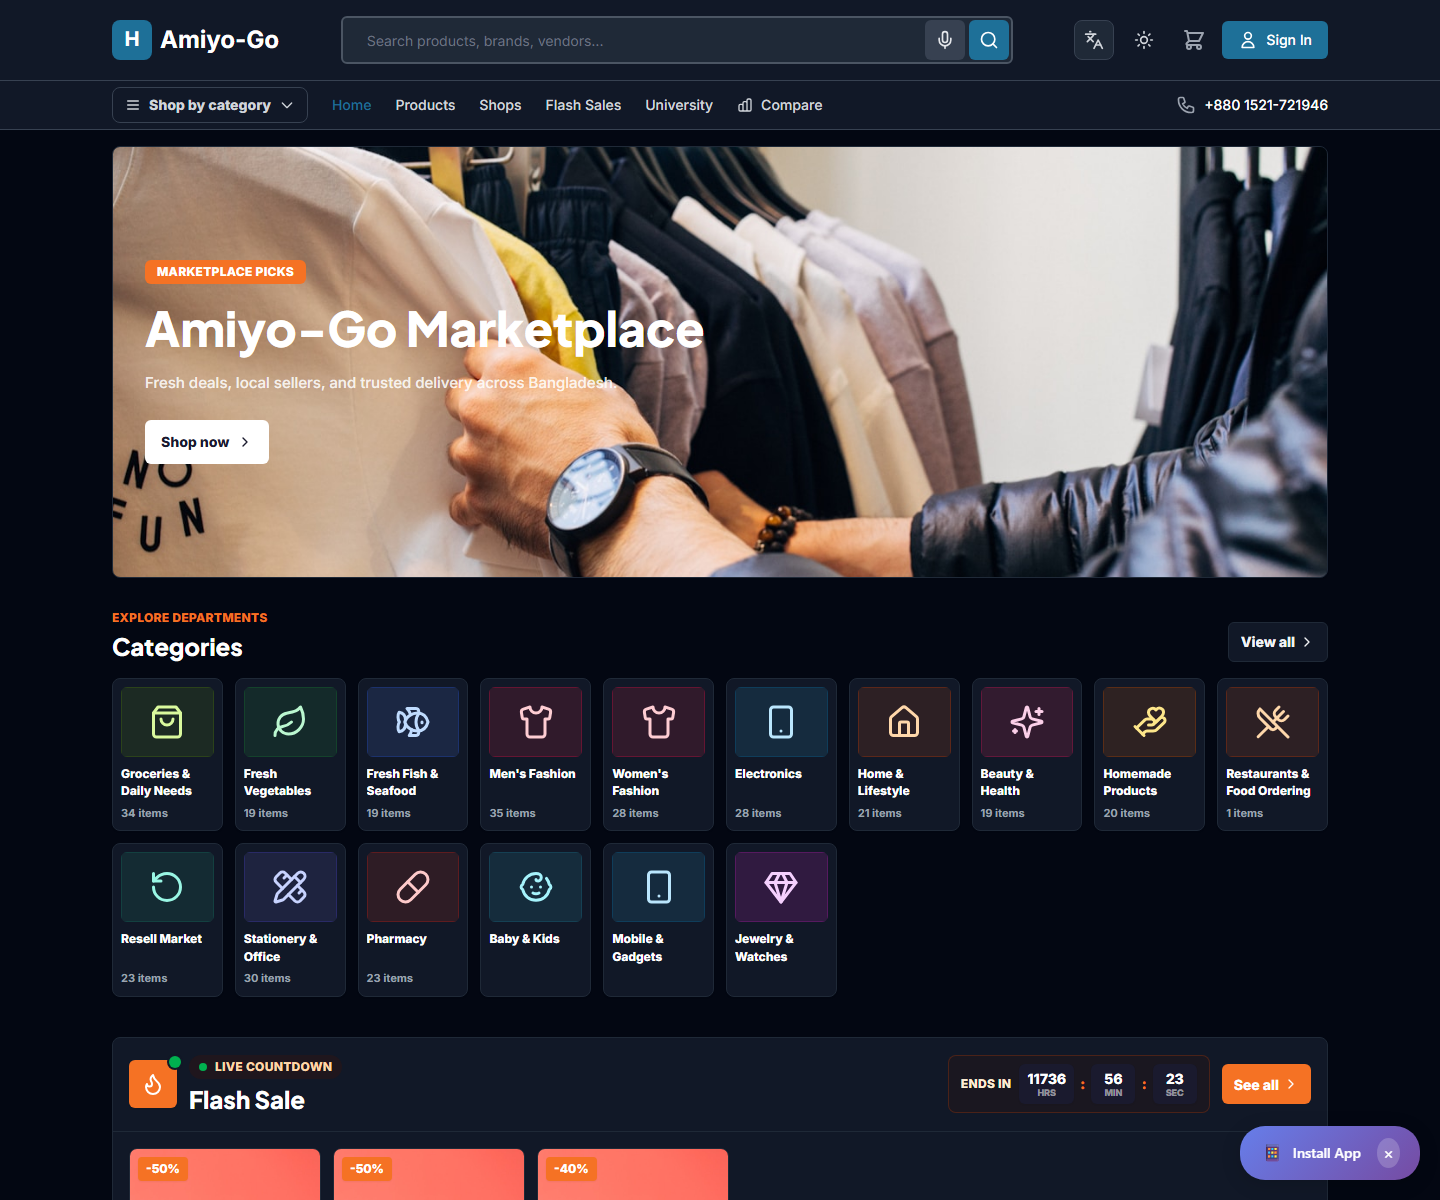
\includegraphics[width=\linewidth,height=0.58\textheight,keepaspectratio]{docs/thesis-screenshots/01-home-desktop.png}
\caption{Customer Home Page}
\end{figure}


English: Shows the modern marketplace landing page, controlled promotional sections, product discovery, and customer entry points.


বাংলা: এখানে আধুনিক মার্কেটপ্লেস হোমপেজ, অ্যাডমিন-কন্ট্রোলড প্রমোশন সেকশন, পণ্য খোঁজা এবং কাস্টমার এন্ট্রি পয়েন্ট দেখা যায়।


\subsection{Screenshot 2: Customer University}

\begin{figure}[htbp]
\centering
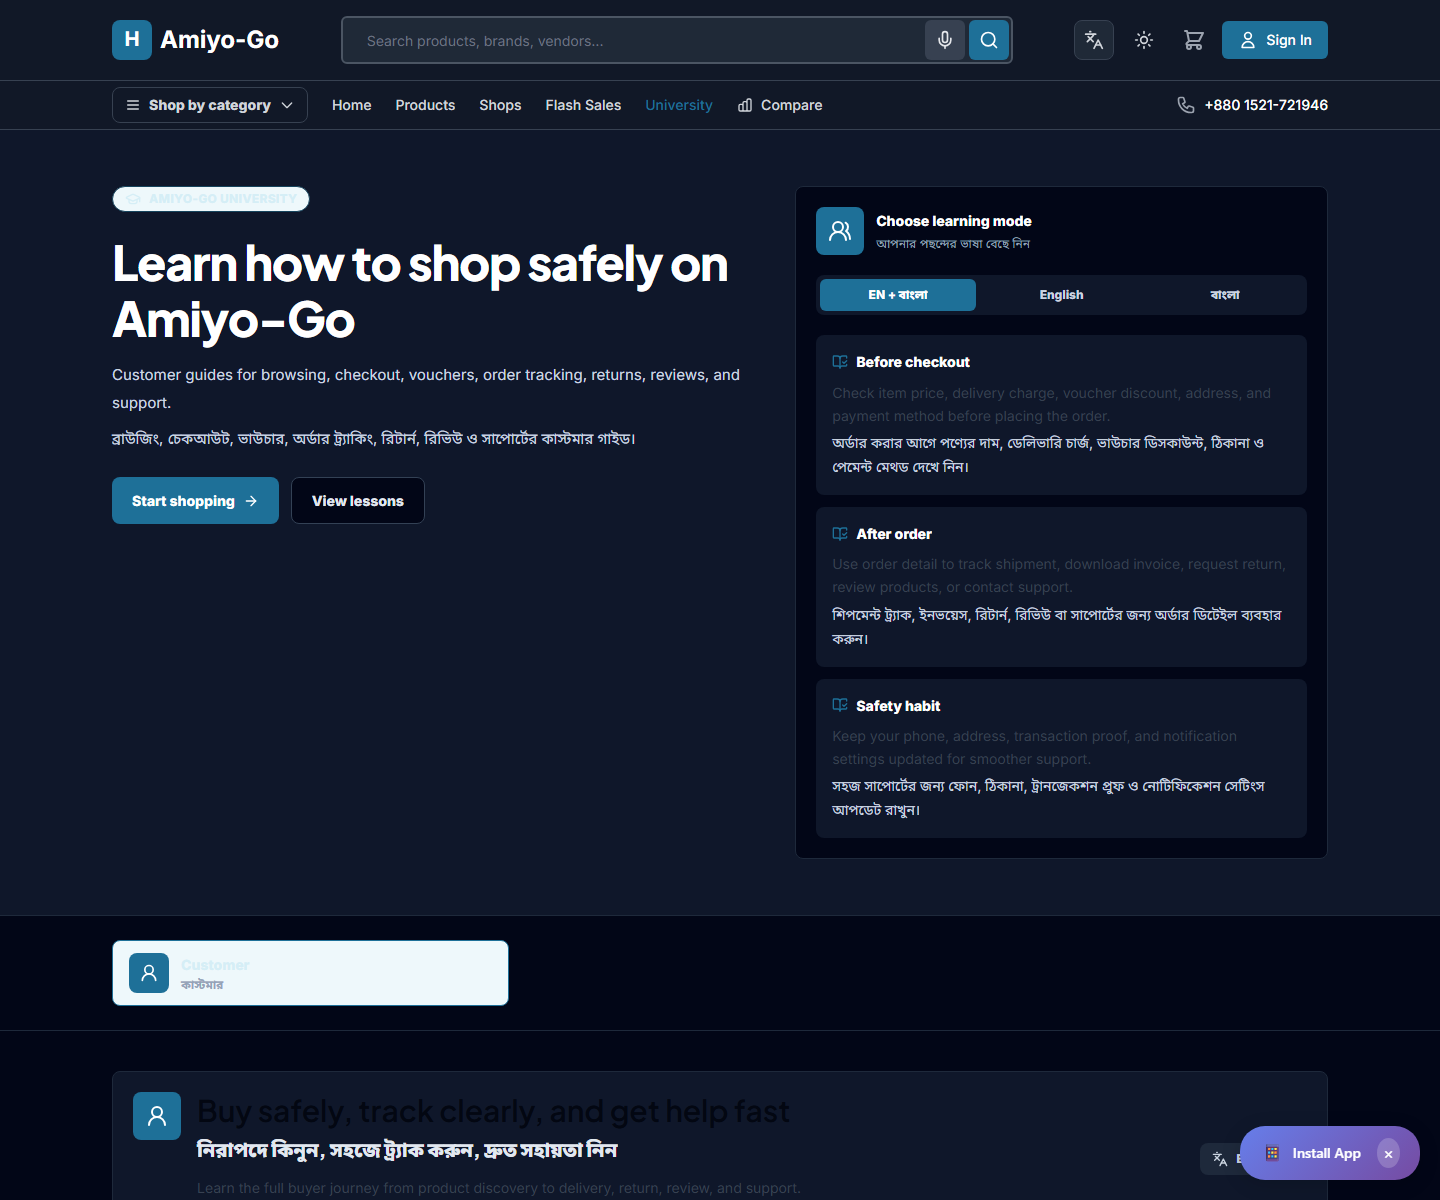
\includegraphics[width=\linewidth,height=0.58\textheight,keepaspectratio]{docs/thesis-screenshots/02-customer-university.png}
\caption{Customer University}
\end{figure}


English: Shows the customer learning center. Public users see only safe customer education, while vendor/admin operating lessons stay behind protected role routes.


বাংলা: এটি কাস্টমার লার্নিং সেন্টার দেখায়। পাবলিক ইউজার শুধু নিরাপদ কাস্টমার গাইড দেখে, ভেন্ডর/অ্যাডমিন অপারেশন গাইড protected role route-এর ভিতরে থাকে।


\subsection{Screenshot 3: Shop Discovery}

\begin{figure}[htbp]
\centering
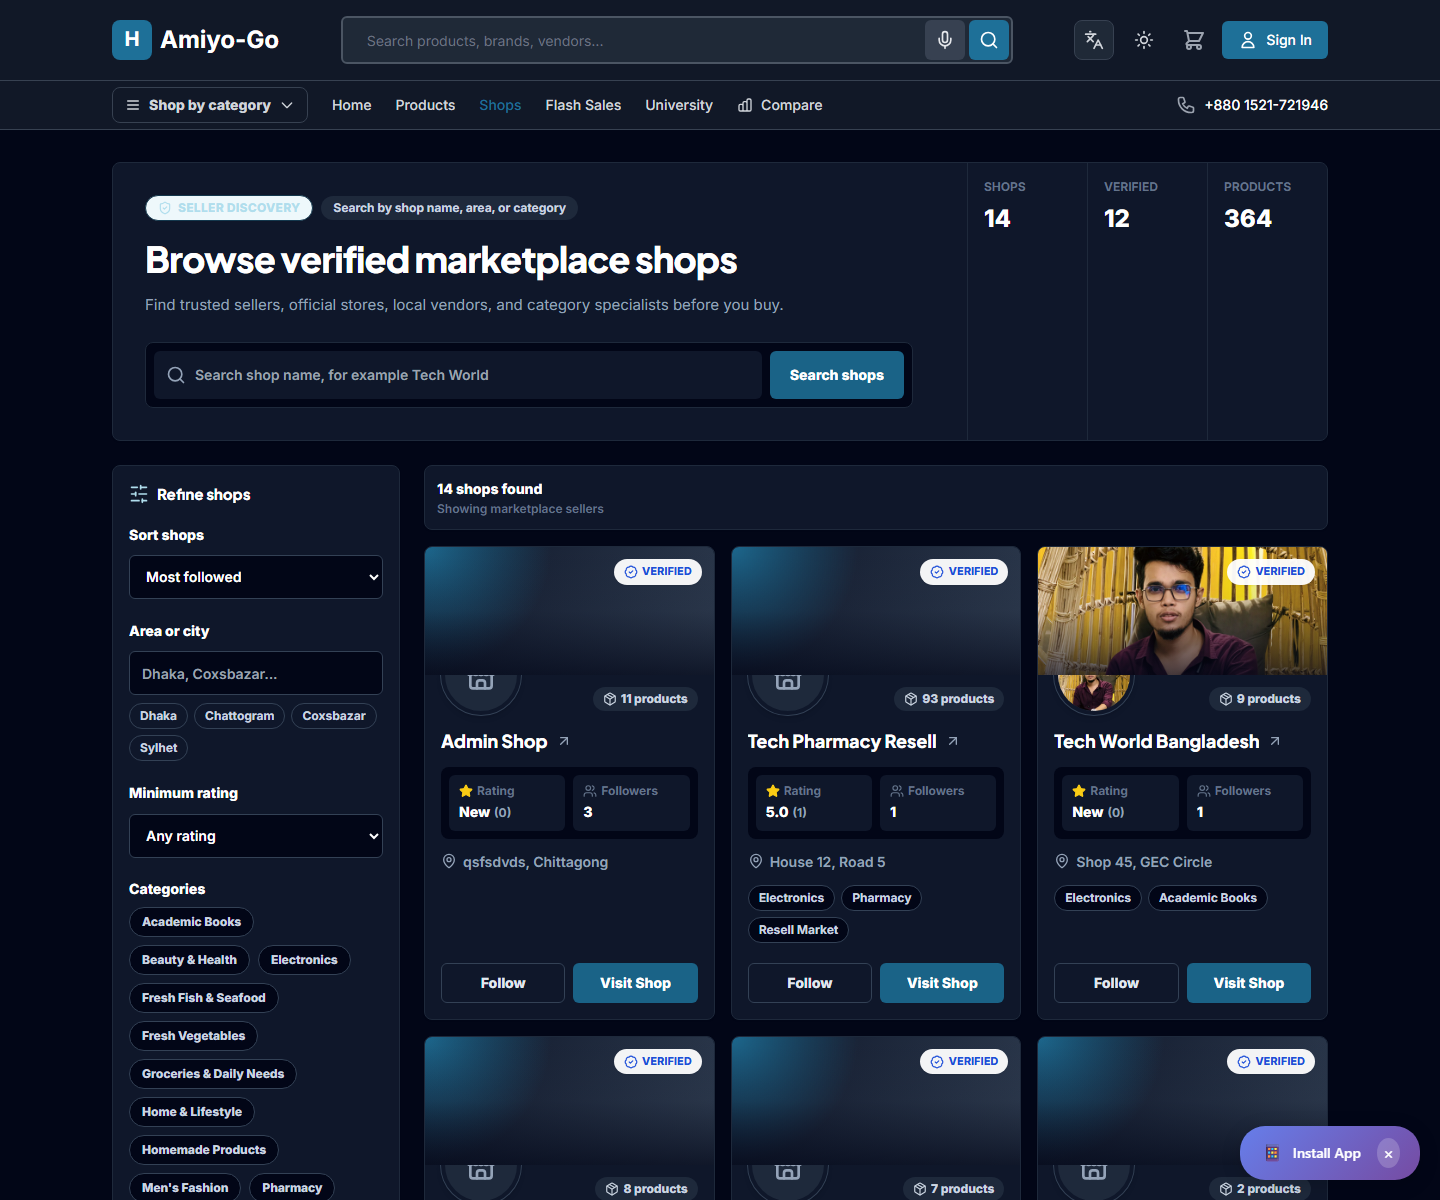
\includegraphics[width=\linewidth,height=0.58\textheight,keepaspectratio]{docs/thesis-screenshots/03-shops-discovery.png}
\caption{Shop Discovery}
\end{figure}


English: Shows public shop browsing, shop search, filters, ratings, follower signals, and storefront navigation.


বাংলা: এখানে পাবলিক শপ ব্রাউজিং, শপ সার্চ, ফিল্টার, রেটিং, ফলোয়ার সিগন্যাল এবং storefront navigation দেখা যায়।


\subsection{Screenshot 4: Account Registration}

\begin{figure}[htbp]
\centering
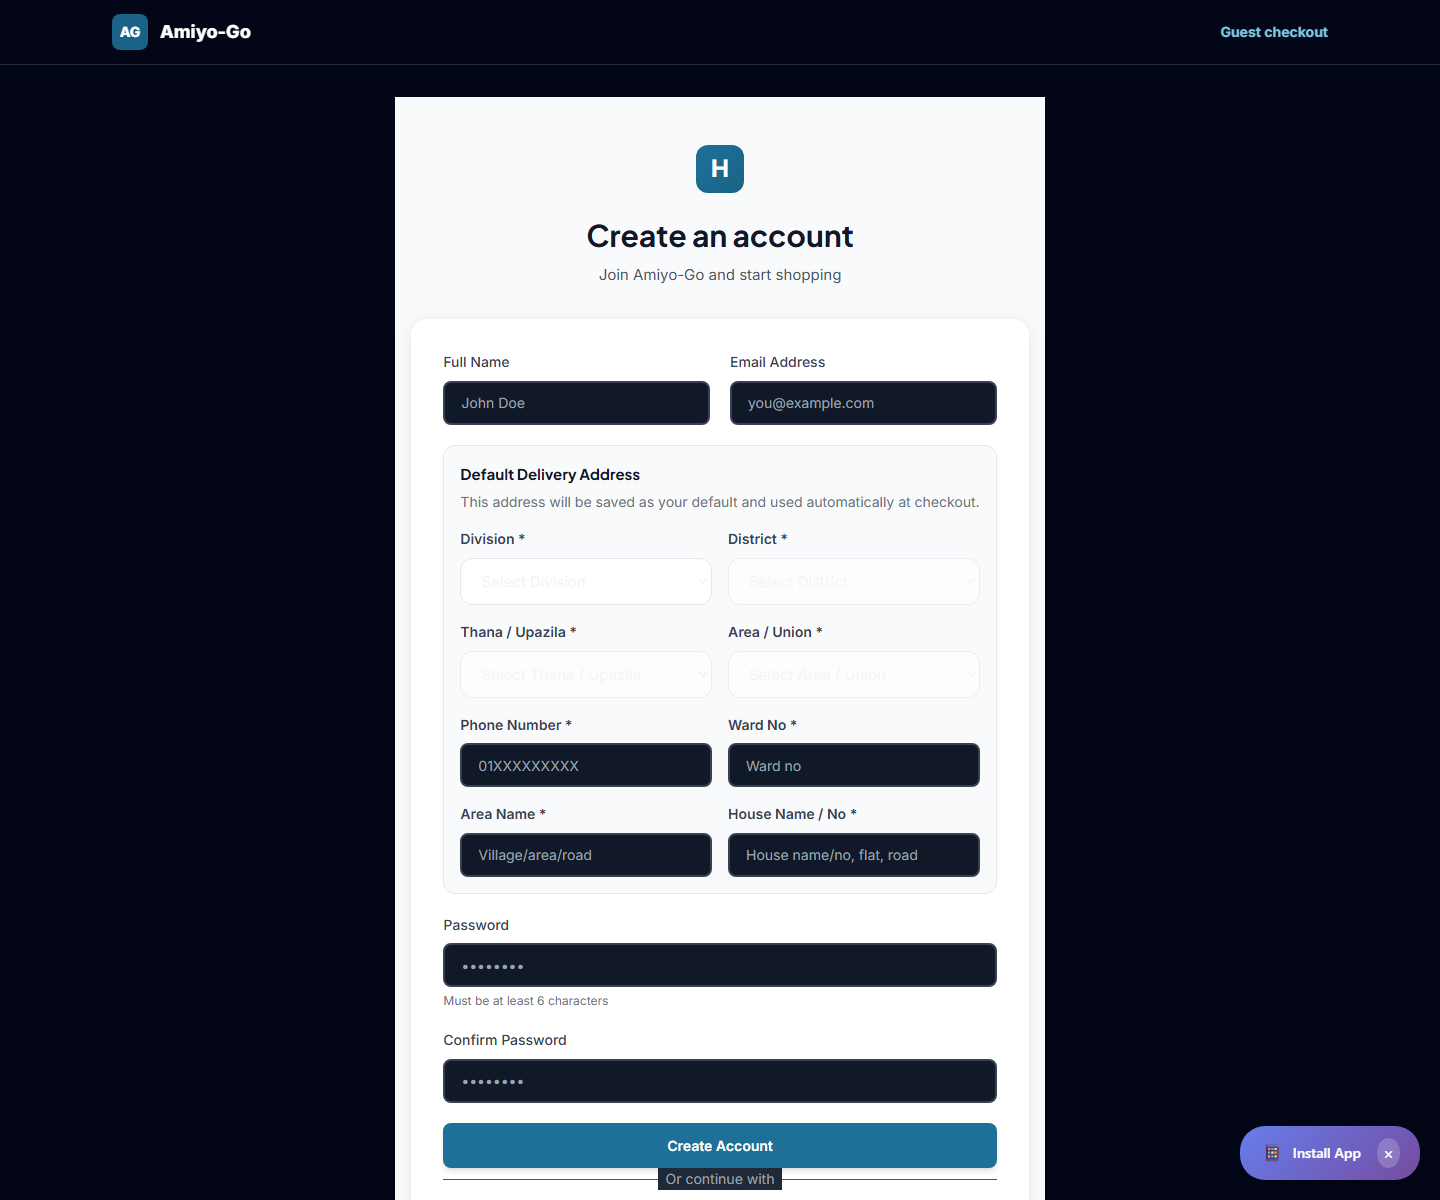
\includegraphics[width=\linewidth,height=0.58\textheight,keepaspectratio]{docs/thesis-screenshots/04-account-registration.png}
\caption{Account Registration}
\end{figure}


English: Shows account creation and address capture, which connects identity, delivery, checkout, order history, and support.


বাংলা: এটি account creation এবং address capture দেখায়, যা identity, delivery, checkout, order history এবং support-এর সাথে যুক্ত।


\subsection{Screenshot 5: Login And Protected Access}

\begin{figure}[htbp]
\centering
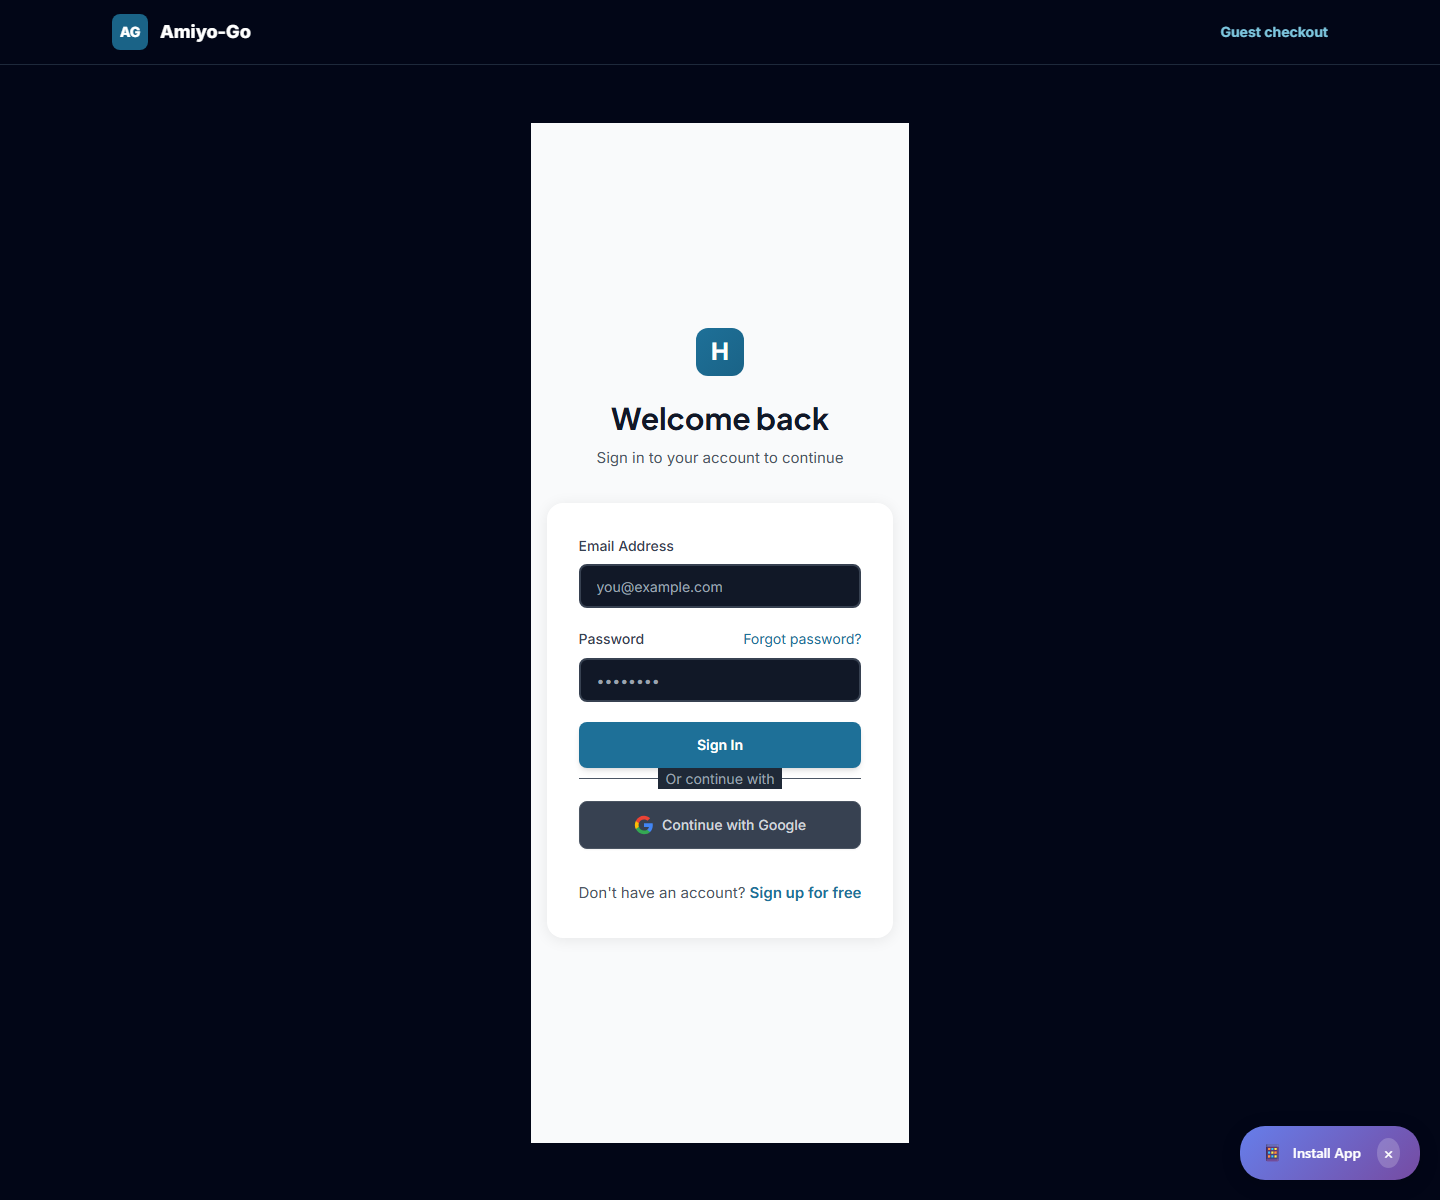
\includegraphics[width=\linewidth,height=0.58\textheight,keepaspectratio]{docs/thesis-screenshots/05-login-access.png}
\caption{Login And Protected Access}
\end{figure}


English: Shows authentication entry. After login, route guards decide whether the user enters customer, vendor, or admin workflows.


বাংলা: এটি authentication entry দেখায়। লগইনের পরে route guard ঠিক করে user customer, vendor নাকি admin workflow-তে যাবে।


\subsection{Screenshot 6: Mobile Home Experience}

\begin{figure}[htbp]
\centering
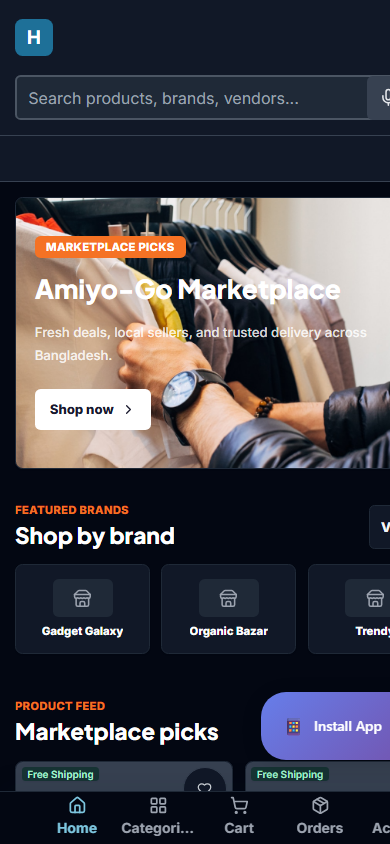
\includegraphics[width=\linewidth,height=0.58\textheight,keepaspectratio]{docs/thesis-screenshots/06-home-mobile.png}
\caption{Mobile Home Experience}
\end{figure}


English: Shows the responsive marketplace experience for mobile users, including compressed discovery sections and PWA-friendly layout.


বাংলা: এটি mobile user-এর responsive marketplace experience দেখায়, যেখানে compact discovery section এবং PWA-friendly layout আছে।


\chapter{Combined Source Documents}

The following sections include the project's existing documentation files in one continuous PDF.


\chapter{Thesis Documentation}

Source file: AMIYO\_GO\_THESIS\_DOCUMENTATION.md


Main project thesis with architecture, screenshots, role workflows, testing, deployment, and bilingual operating narrative.


\chapter{Amiyo-Go Marketplace Thesis Documentation}

\textbf{Project:} Amiyo-Go Multi-Vendor Marketplace

\textbf{Document type:} Thesis-style technical documentation

\textbf{Last updated:} 2026-06-04

\textbf{Prepared for:} Product, engineering, operations, vendor, and admin review


\begin{CodeBlock}
---
\end{CodeBlock}

\section{Abstract}

Amiyo-Go is a role-based multi-vendor marketplace system designed to support customer shopping, vendor seller-center operations, and admin marketplace governance. The project has evolved beyond a simple ecommerce catalog into a marketplace operating system with modules for catalog management, vendor onboarding, order fulfillment, courier workflow, returns, payments, promotions, trust and safety, analytics, staff permissions, and documentation/training.


The application follows a modular monolith architecture. The frontend is built with React, React Router, Tailwind CSS, reusable UI components, and role-specific layouts. The backend is a Node.js and Express API layer using MongoDB through Mongoose and native MongoDB access. Selected background workflows use BullMQ/Redis where configured. The system includes adapter-ready integrations for courier providers, payment providers, notification channels, object storage, and search provider abstraction.


This documentation records the full implementation scope, current architecture, feature inventory, role workflows, data model map, API surface, quality practices, deployment notes, known limitations, and future production-hardening roadmap. It is intended to work as a project thesis, handover document, and production-readiness reference.


\section{Keywords}

Marketplace, ecommerce, multi-vendor, seller center, admin dashboard, logistics, COD, returns, trust and safety, analytics, promotions, React, Node.js, Express, MongoDB, Firebase, BullMQ.


\begin{CodeBlock}
---
\end{CodeBlock}

\section{Table of Contents}

\begin{enumerate}
\item Introduction
\item Project Goals and Scope
\item Stakeholder and Role Analysis
\item Technology Stack
\item System Architecture and UI Screenshots
\item Frontend Architecture
\item Backend Architecture
\item Database and Persistence Model
\item Feature Documentation by Role
\item Business Workflows
\item API and Service Map
\item Security, Trust, and Permissions
\item Logistics and Courier Integration
\item Promotions, Growth, and Personalization
\item Analytics and Reporting
\item Testing and Quality Assurance
\item Deployment and Environment Configuration
\item Documentation and Training Layer
\item Production-Readiness Assessment
\item Limitations and Future Work
\item Conclusion
\item Appendices
\end{enumerate}

\begin{CodeBlock}
---
\end{CodeBlock}

\chapter{Chapter 1: Introduction}

\section{1.1 Background}

Modern marketplaces are not only product listing websites. They are operational platforms where customers, sellers, and platform operators coordinate through structured workflows. A Daraz-level marketplace needs customer discovery and checkout, seller-center controls, logistics state tracking, finance settlement, dispute handling, campaign tools, analytics, and staff governance.


Amiyo-Go is designed around that concept. The project connects customer shopping actions, vendor operating tools, and admin governance into one system. The core value is not only that products can be purchased, but that the marketplace can be managed after the order is placed.


\section{1.2 Problem Statement}

A normal ecommerce application usually solves only these problems:


\begin{itemize}
\item Display products.
\item Add products to cart.
\item Place an order.
\item Let an admin view orders.
\end{itemize}

A real marketplace must solve many more:


\begin{itemize}
\item Sellers need onboarding, KYC, product moderation, stock management, packing, finance, promotions, and reputation tools.
\item Customers need trustworthy shopping, order tracking, invoices, returns, refunds, support, reviews, saved addresses, alerts, loyalty, and notifications.
\item Admins need vendor approval, moderation queues, dispatch controls, COD reconciliation, payment verification, payout management, trust and safety, analytics, staff permissions, and audit logs.
\item Operators need clear documentation and training so each role understands what they should see and do.
\end{itemize}

Amiyo-Go addresses these needs through a modular marketplace workflow.


\section{1.3 Project Aim}

The aim of Amiyo-Go is to provide a production-oriented marketplace foundation that can operate with manual workflows first and gradually attach paid/external integrations such as courier APIs, payment gateways, SMS providers, object storage, and search engines.


\section{1.4 Thesis Objective}

This document has four objectives:


\begin{enumerate}
\item Explain the complete project architecture.
\item Document all major customer, vendor, and admin features.
\item Record operational workflows and implementation status.
\item Provide a production-readiness reference for future hardening.
\end{enumerate}

\begin{CodeBlock}
---
\end{CodeBlock}

\chapter{Chapter 2: Project Goals and Scope}

\section{2.1 Functional Goals}

The main functional goals are:


\begin{itemize}
\item Build a three-role marketplace: customer, vendor, and admin.
\item Allow customers to browse, search, purchase, track, return, review, and get support.
\item Allow vendors to manage shop, KYC, catalog, inventory, orders, fulfillment, returns, finance, marketing, Q\&A, reviews, and reports.
\item Allow admins to manage vendors, products, orders, returns, payouts, COD, logistics, promotions, trust, staff, analytics, and platform settings.
\item Support customer-facing shop storefronts with follow/unfollow and vendor products.
\item Support marketplace growth through promotions, flash sales, loyalty, recommendations, alerts, and notifications.
\item Support logistics through internal shipment state machines and adapter-ready courier booking.
\item Support role learning through Amiyo-Go University with protected vendor/admin learning content.
\end{itemize}

\section{2.2 Non-Functional Goals}

Important non-functional goals include:


\begin{itemize}
\item Maintainable modular monolith design.
\item Role-based access control.
\item Secure API boundaries.
\item Responsive frontend UI.
\item Progressive Web App readiness.
\item Auditable admin and finance actions.
\item Extensible integration adapters.
\item Documentation-first handover.
\item Testable frontend and backend modules.
\end{itemize}

\section{2.3 Scope Boundary}

The project currently includes many production-grade foundations, but some external systems remain environment-dependent:


\begin{itemize}
\item MongoDB is the current database. PostgreSQL is not the current implementation.
\item Redis and BullMQ exist for selected background workflows, but they are not yet universal for every event.
\item Courier APIs are adapter-ready. Manual and internal courier workflows remain valid without paid courier API activation.
\item Payment provider adapters exist, but production payment depth depends on provider credentials and webhook configuration.
\item Email, push, and optional SMS rely on configured providers.
\item Object storage/upload provider behavior depends on environment configuration.
\end{itemize}

\begin{CodeBlock}
---
\end{CodeBlock}

\chapter{Chapter 3: Stakeholder and Role Analysis}

\section{3.1 Customer}

The customer is the buyer role. Customers use the marketplace to discover products, compare options, place orders, track delivery, request returns, review products, and contact support.


Customer priorities:


\begin{itemize}
\item Trustworthy product information.
\item Clear prices and discounts.
\item Smooth checkout.
\item Accurate order tracking.
\item Easy returns and support.
\item Useful recommendations and alerts.
\end{itemize}

\section{3.2 Vendor}

The vendor is the seller role. Vendors use Amiyo-Go as a seller center to manage shop identity, products, stock, orders, packing, dispatch, returns, finance, promotions, reviews, and support communication.


Vendor priorities:


\begin{itemize}
\item Clear onboarding and KYC status.
\item Product approval workflow.
\item Fast order handling.
\item Finance clarity.
\item Campaign and voucher tools.
\item Shop reputation and customer communication.
\end{itemize}

\section{3.3 Admin}

The admin is the marketplace operator role. Admins control the platform through queues, policies, settings, staff permissions, audit logs, moderation, logistics, finance, trust, and analytics.


Admin priorities:


\begin{itemize}
\item Central visibility.
\item Exception handling.
\item Approval workflows.
\item Fraud and dispute control.
\item Revenue and payout accuracy.
\item Staff access governance.
\item Operational dashboards.
\end{itemize}

\begin{CodeBlock}
---
\end{CodeBlock}

\chapter{Chapter 4: Technology Stack}

\section{4.1 Frontend Stack}

\begin{CodeBlock}
| Area | Technology |
\end{CodeBlock}
\begin{CodeBlock}
| --- | --- |
\end{CodeBlock}
\begin{CodeBlock}
| Framework | React |
\end{CodeBlock}
\begin{CodeBlock}
| Router | React Router |
\end{CodeBlock}
\begin{CodeBlock}
| Build tool | Vite |
\end{CodeBlock}
\begin{CodeBlock}
| Styling | Tailwind CSS and reusable UI components |
\end{CodeBlock}
\begin{CodeBlock}
| Icons | lucide-react |
\end{CodeBlock}
\begin{CodeBlock}
| HTTP | axios and fetch patterns |
\end{CodeBlock}
\begin{CodeBlock}
| Forms | react-hook-form where used |
\end{CodeBlock}
\begin{CodeBlock}
| Charts | Chart.js, Recharts |
\end{CodeBlock}
\begin{CodeBlock}
| Maps | Leaflet and react-leaflet |
\end{CodeBlock}
\begin{CodeBlock}
| Notifications | react-hot-toast, push subscription UI |
\end{CodeBlock}
\begin{CodeBlock}
| i18n | i18next and react-i18next |
\end{CodeBlock}
\begin{CodeBlock}
| PWA | Manifest and service worker support |
\end{CodeBlock}
\begin{CodeBlock}
| Tests | Jest, React Testing Library |
\end{CodeBlock}

\section{4.2 Backend Stack}

\begin{CodeBlock}
| Area | Technology |
\end{CodeBlock}
\begin{CodeBlock}
| --- | --- |
\end{CodeBlock}
\begin{CodeBlock}
| Runtime | Node.js |
\end{CodeBlock}
\begin{CodeBlock}
| API framework | Express |
\end{CodeBlock}
\begin{CodeBlock}
| Database | MongoDB |
\end{CodeBlock}
\begin{CodeBlock}
| ODM | Mongoose |
\end{CodeBlock}
\begin{CodeBlock}
| Native database access | mongodb package where needed |
\end{CodeBlock}
\begin{CodeBlock}
| Auth integration | Firebase Admin SDK |
\end{CodeBlock}
\begin{CodeBlock}
| File upload | multer, upload service, storage adapters |
\end{CodeBlock}
\begin{CodeBlock}
| PDF generation | pdfkit |
\end{CodeBlock}
\begin{CodeBlock}
| Queues | BullMQ and Redis where configured |
\end{CodeBlock}
\begin{CodeBlock}
| Email | nodemailer and email services |
\end{CodeBlock}
\begin{CodeBlock}
| Push | web-push |
\end{CodeBlock}
\begin{CodeBlock}
| Payments | Provider adapter services including bKash/Nagad/SSLCommerz/Stripe patterns |
\end{CodeBlock}
\begin{CodeBlock}
| Courier | Courier provider service and Amiyo Delivery integration service |
\end{CodeBlock}
\begin{CodeBlock}
| Security | helmet, cors, rate limit, sanitization |
\end{CodeBlock}
\begin{CodeBlock}
| Logging | winston |
\end{CodeBlock}
\begin{CodeBlock}
| Tests | Jest, Supertest |
\end{CodeBlock}

\section{4.3 Infrastructure and Integrations}

External or optional integrations include:


\begin{itemize}
\item Firebase authentication and admin claims.
\item MongoDB Atlas or local MongoDB.
\item Redis for queues where enabled.
\item Email provider.
\item Web push provider keys.
\item Courier providers such as RedX, Steadfast, local/internal delivery, and Amiyo Delivery integration.
\item Payment gateways and manual payment verification.
\item Object storage adapters.
\end{itemize}

\begin{CodeBlock}
---
\end{CodeBlock}

\chapter{Chapter 5: System Architecture}

\section{5.1 Architectural Style}

Amiyo-Go uses a modular monolith architecture. All business domains are inside one backend application, but each major domain has its own routes, controllers, models, services, utilities, and frontend pages.


This architecture is appropriate because:


\begin{itemize}
\item It is easier to develop and test than microservices.
\item It keeps cross-domain workflows in one codebase.
\item It allows future extraction of heavy modules if scale demands it.
\item It supports fast iteration for marketplace features.
\end{itemize}

\section{5.2 High-Level System Flow}

\begin{CodeBlock}
Customer Web App / Vendor Dashboard / Admin Dashboard
-> React frontend with role-based layouts and guards
-> Express API
-> Domain route modules
-> Services and utilities
-> MongoDB collections/models
-> Optional queues, storage, courier, payment, email, push
\end{CodeBlock}

\section{5.3 Main Backend Domains}

The backend registers route groups for:


\begin{itemize}
\item Products and catalog.
\item Search and discovery.
\item Categories and dynamic categories.
\item Orders and vendor orders.
\item Shipments and logistics.
\item Users, accounts, addresses.
\item Wishlist and alerts.
\item Reviews and Q\&A.
\item Coupons, vouchers, offers, campaigns, promotions.
\item Returns and refunds.
\item Payments and webhooks.
\item Support and chats.
\item Flash sales and recommendations.
\item Growth systems.
\item Trust and safety.
\item Platform settings.
\item Delivery settings and courier rules.
\item Vendor staff, KYC, shop, products, logistics, finance, growth.
\item Admin users, vendors, products, payments, banners, settings, staff, COD, reviews, finance, payouts, analytics, logistics, customers, platform, audit.
\end{itemize}

\section{5.4 Frontend Role Layouts}

The frontend separates role experience through:


\begin{itemize}
\item Main/customer layout.
\item Vendor layout.
\item Admin layout.
\item Route guards.
\item Role-specific navigation.
\item Protected University pages for vendor/admin training.
\end{itemize}

\section{5.5 Screenshot Walkthrough and How It Works}

This screenshot set was captured from the running frontend on 2026-06-04. It intentionally uses public and access pages only, so the PDF does not expose private admin/vendor data or real customer records. Protected vendor/admin dashboards are documented through workflows and route descriptions instead of unauthenticated screenshots.


এই স্ক্রিনশটগুলো ২০২৬-০৬-০৪ তারিখে রানিং frontend থেকে নেওয়া হয়েছে। এখানে শুধু public/access page ব্যবহার করা হয়েছে, তাই PDF-এ private admin/vendor data বা real customer record প্রকাশ করা হয়নি। Protected vendor/admin dashboard স্ক্রিনশটের বদলে workflow এবং route description দিয়ে ব্যাখ্যা করা হয়েছে।


\subsection{Figure 1: Customer Home Page}

\begin{figure}[htbp]
\centering
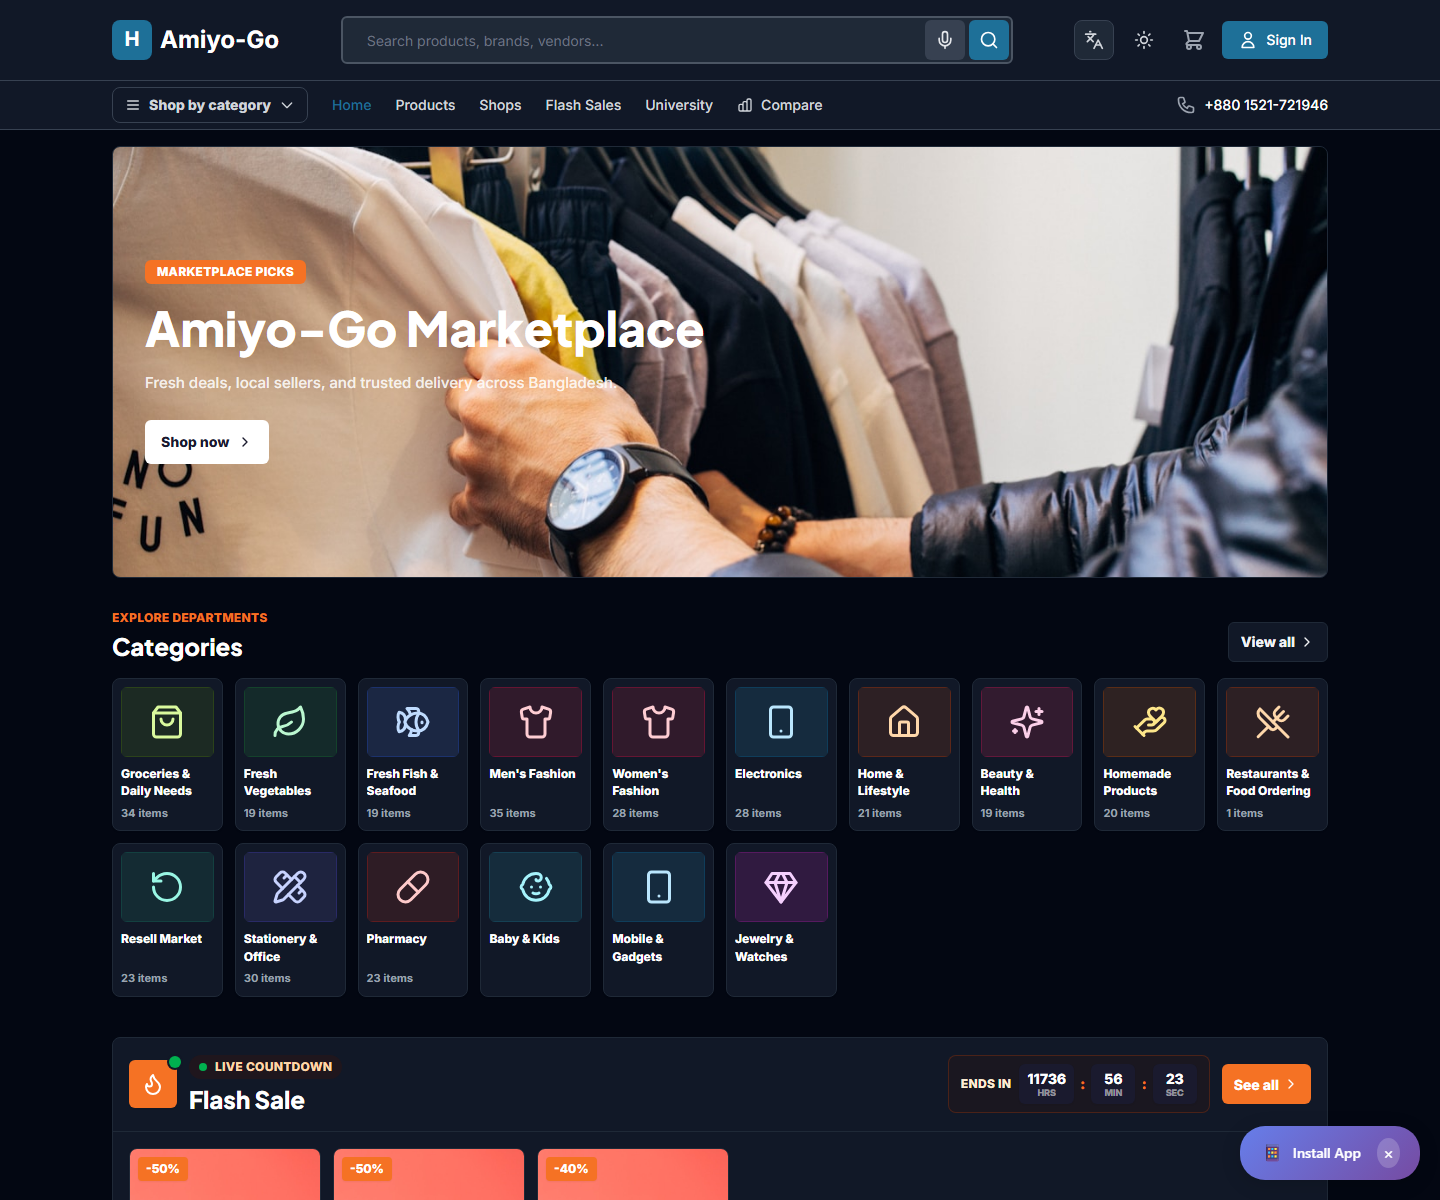
\includegraphics[width=\linewidth,height=0.58\textheight,keepaspectratio]{docs/thesis-screenshots/01-home-desktop.png}
\caption{Customer home page with modern marketplace sections}
\end{figure}


\textbf{How it works in English:}


\begin{itemize}
\item The customer enters through the home page.
\item The header gives search, category navigation, product links, shops, flash sales, compare, language, theme, cart, and sign-in access.
\item The hero area promotes the marketplace and sends users into shopping.
\item Category, flash sale, product, and shop sections help users discover products quickly.
\item Admin-controlled banners and sections can change the front page without code changes.
\end{itemize}

\textbf{কীভাবে কাজ করে বাংলায়:}


\begin{itemize}
\item কাস্টমার home page দিয়ে marketplace-এ প্রবেশ করে।
\item Header থেকে search, category, product, shops, flash sale, compare, language, theme, cart এবং sign-in access পাওয়া যায়।
\item Hero section marketplace offer দেখায় এবং user-কে shopping flow-তে নিয়ে যায়।
\item Category, flash sale, product এবং shop section দ্রুত product discovery করতে সাহায্য করে।
\item Admin-controlled banner এবং section code change ছাড়াই homepage update করতে পারে।
\end{itemize}

\subsection{Figure 2: Customer Learning Center}

\begin{figure}[htbp]
\centering
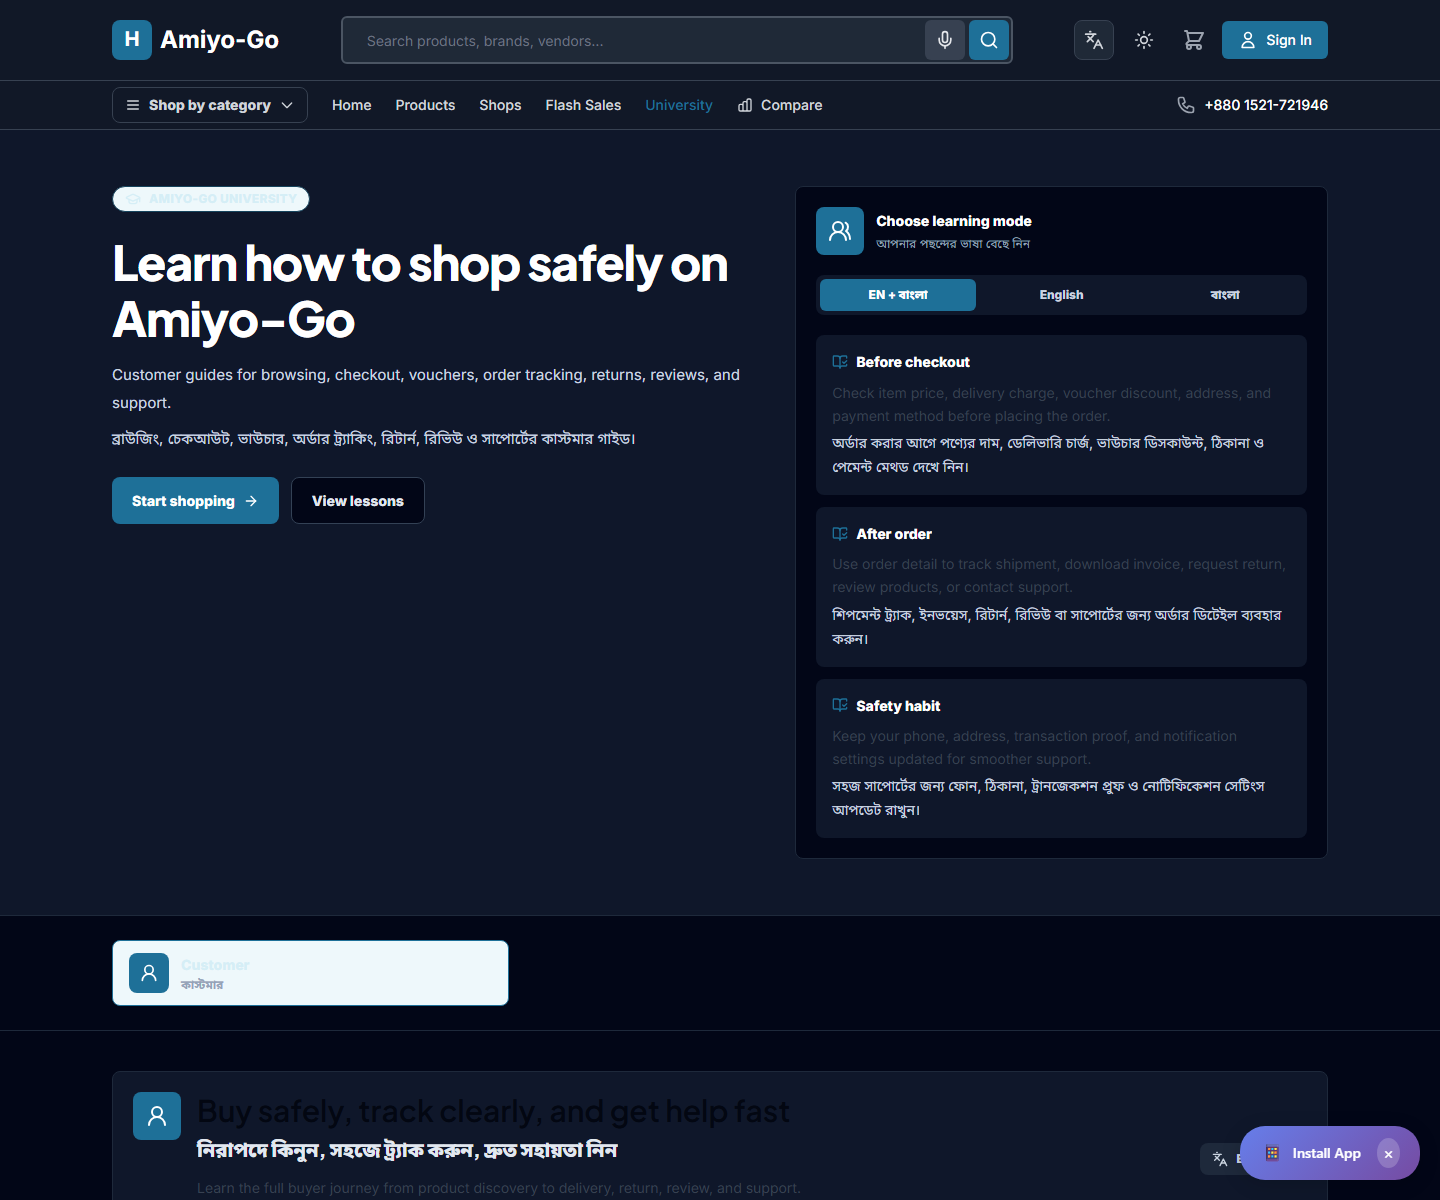
\includegraphics[width=\linewidth,height=0.58\textheight,keepaspectratio]{docs/thesis-screenshots/02-customer-university.png}
\caption{Customer-only Amiyo-Go University page}
\end{figure}


\textbf{How it works in English:}


\begin{itemize}
\item Public users only see customer learning content on \texttt{/university}.
\item Vendor and admin operating lessons are not bundled into the public route.
\item Customers learn checkout, vouchers, order tracking, returns, reviews, and support.
\item Language mode supports English, Bangla, or both together.
\end{itemize}

\textbf{কীভাবে কাজ করে বাংলায়:}


\begin{itemize}
\item Public user \texttt{/university} পেজে শুধু customer guide দেখে।
\item Vendor/admin operating lesson public route-এ bundle করা হয় না।
\item Customer checkout, voucher, order tracking, return, review এবং support শেখে।
\item Language mode English, Bangla বা দুই ভাষা একসাথে support করে।
\end{itemize}

\subsection{Figure 3: Shop Discovery}

\begin{figure}[htbp]
\centering
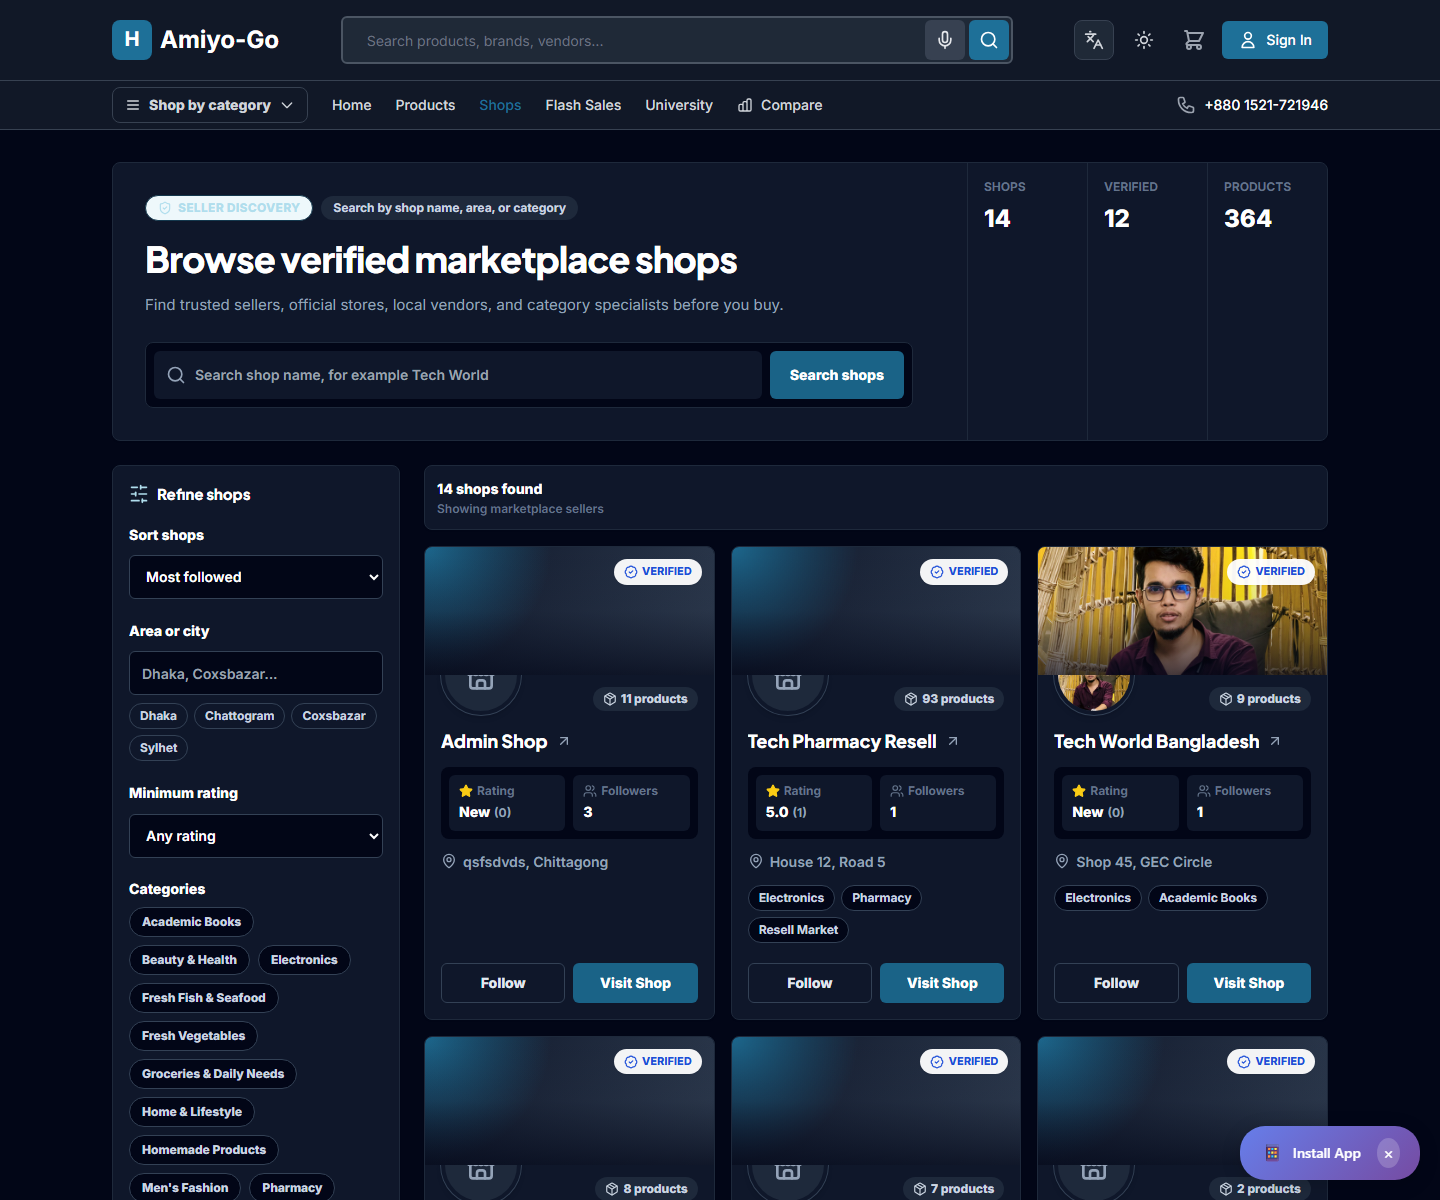
\includegraphics[width=\linewidth,height=0.58\textheight,keepaspectratio]{docs/thesis-screenshots/03-shops-discovery.png}
\caption{Shop discovery page with filters, shop cards, and follow action}
\end{figure}


\textbf{How it works in English:}


\begin{itemize}
\item Customers can browse verified marketplace shops.
\item Search supports shop name, area, and category intent.
\item Filters allow sorting by popularity, location, rating, and category.
\item Each shop card shows trust signals, product count, follower count, location, and visit/follow actions.
\item The backend \texttt{/api/shops} route returns safe public vendor fields only.
\end{itemize}

\textbf{কীভাবে কাজ করে বাংলায়:}


\begin{itemize}
\item Customer verified marketplace shop browse করতে পারে।
\item Search shop name, area এবং category intent support করে।
\item Filter দিয়ে popularity, location, rating এবং category অনুযায়ী result দেখা যায়।
\item Shop card-এ trust signal, product count, follower count, location, visit এবং follow action থাকে।
\item Backend \texttt{/api/shops} route শুধু safe public vendor field return করে।
\end{itemize}

\subsection{Figure 4: Account Registration and Address Capture}

\begin{figure}[htbp]
\centering
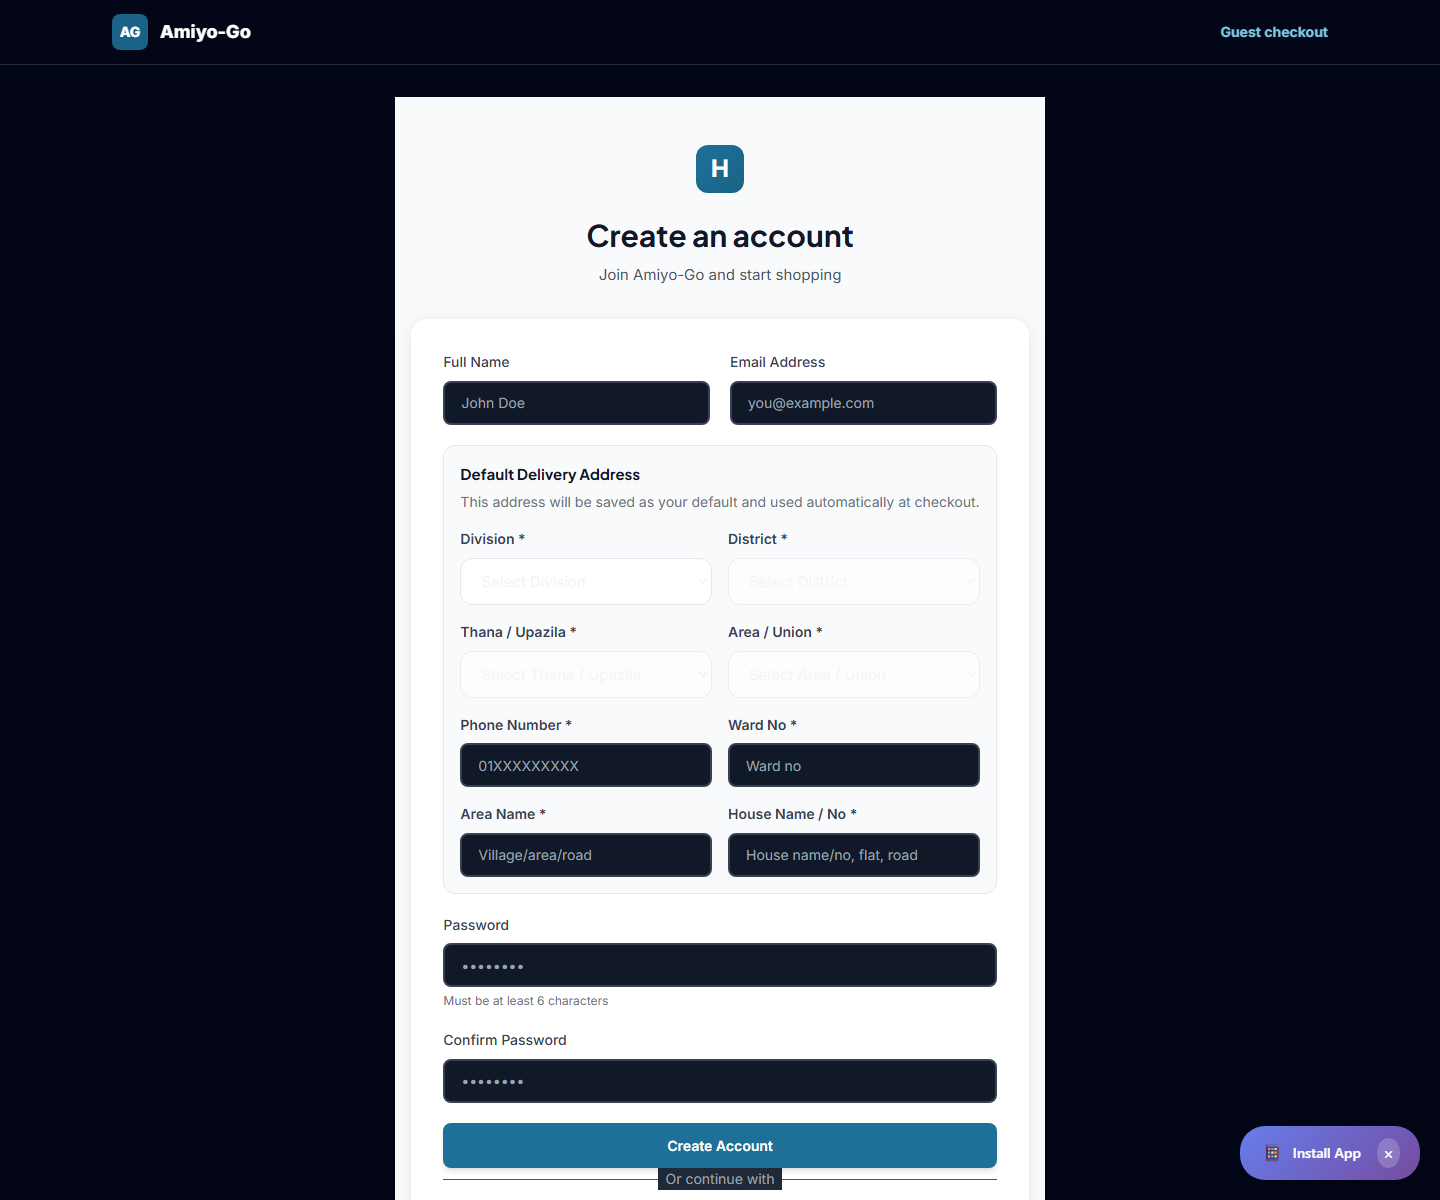
\includegraphics[width=\linewidth,height=0.58\textheight,keepaspectratio]{docs/thesis-screenshots/04-account-registration.png}
\caption{Customer registration page with default address fields}
\end{figure}


\textbf{How it works in English:}


\begin{itemize}
\item A new customer creates an account before using full account features.
\item Registration captures basic identity and default delivery address.
\item Address fields are structured for Bangladesh delivery workflow.
\item The saved address later supports checkout, delivery calculation, courier assignment, and support.
\end{itemize}

\textbf{কীভাবে কাজ করে বাংলায়:}


\begin{itemize}
\item নতুন customer full account feature ব্যবহারের আগে account তৈরি করে।
\item Registration basic identity এবং default delivery address নেয়।
\item Address fields Bangladesh delivery workflow অনুযায়ী structured।
\item Saved address পরে checkout, delivery calculation, courier assignment এবং support-এ ব্যবহার হয়।
\end{itemize}

\subsection{Figure 5: Login and Protected Access}

\begin{figure}[htbp]
\centering
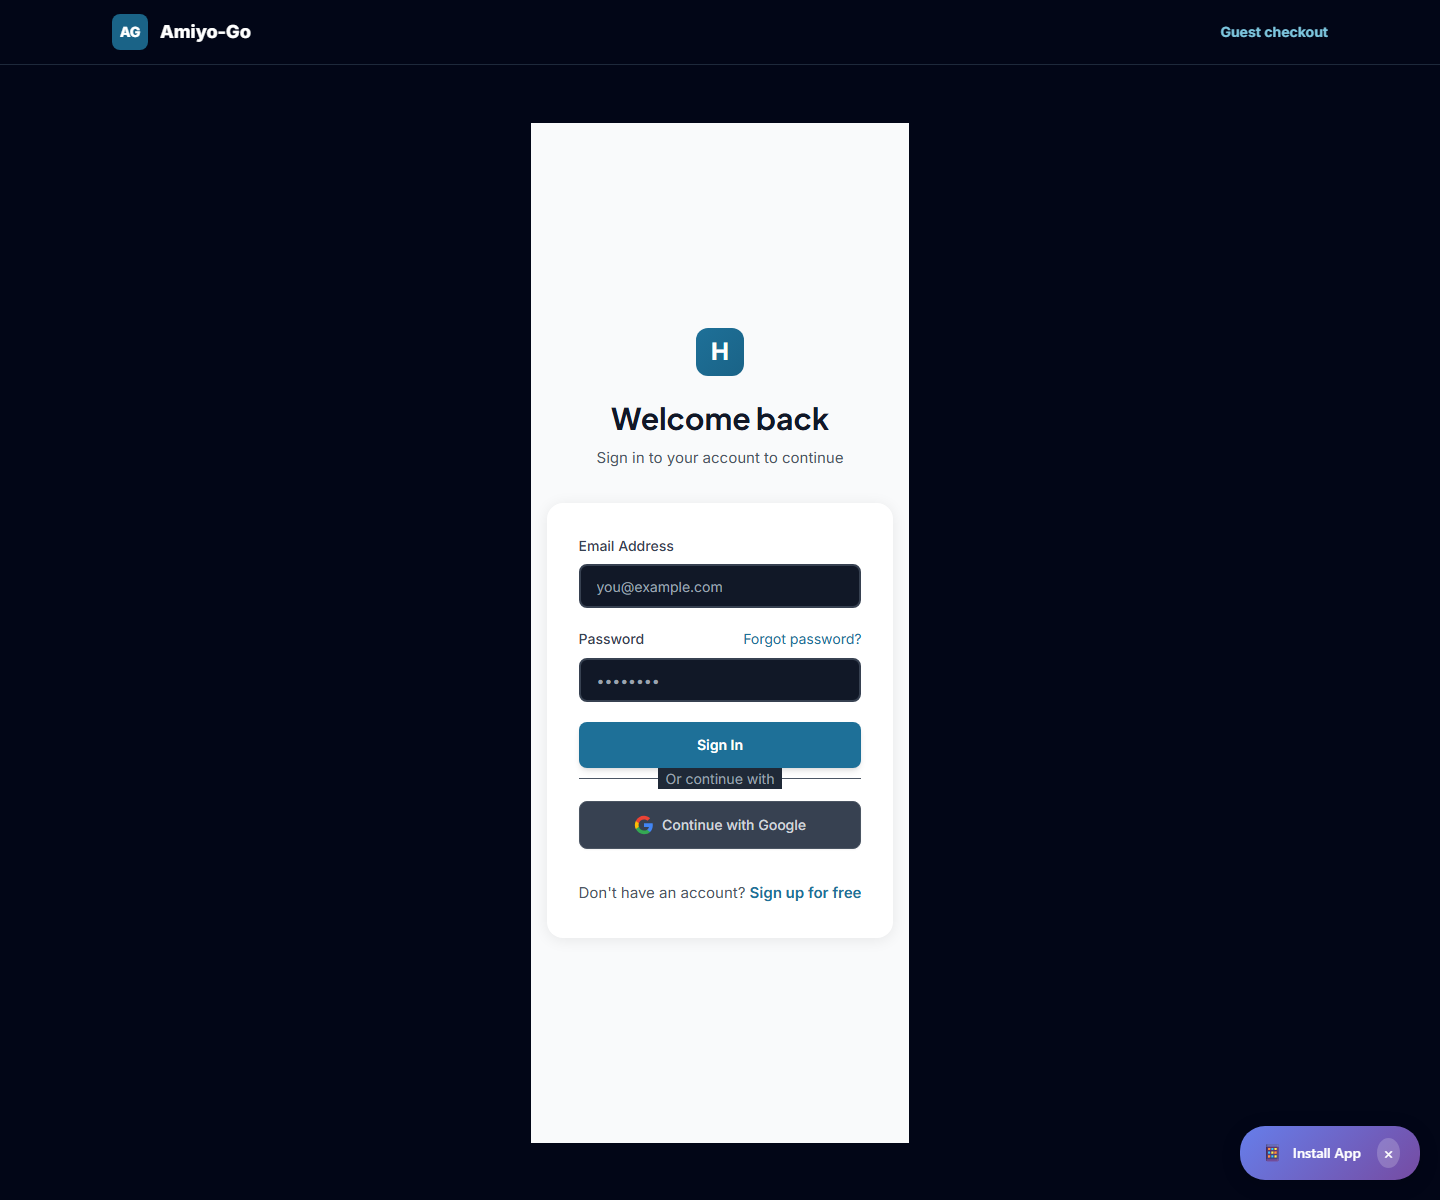
\includegraphics[width=\linewidth,height=0.58\textheight,keepaspectratio]{docs/thesis-screenshots/05-login-access.png}
\caption{Login page for customer, vendor, and admin access}
\end{figure}


\textbf{How it works in English:}


\begin{itemize}
\item Users sign in before accessing protected customer, vendor, or admin pages.
\item Route guards redirect unauthenticated users to login.
\item Admin and vendor pages also check role/permission after authentication.
\item Guest checkout remains available where the project allows it.
\end{itemize}

\textbf{কীভাবে কাজ করে বাংলায়:}


\begin{itemize}
\item Protected customer, vendor বা admin page access করার আগে user sign in করে।
\item Route guard unauthenticated user-কে login page-এ পাঠায়।
\item Admin এবং vendor page authentication-এর পরে role/permission check করে।
\item Project যেখানে allow করে সেখানে guest checkout available থাকে।
\end{itemize}

\subsection{Figure 6: Mobile Home Experience}

\begin{figure}[htbp]
\centering
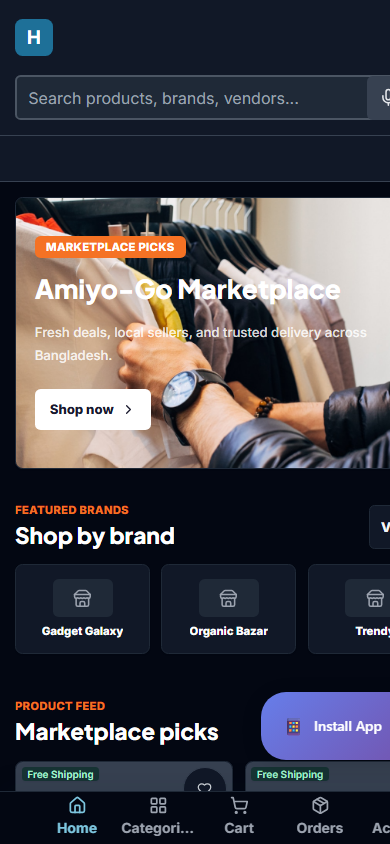
\includegraphics[width=\linewidth,height=0.58\textheight,keepaspectratio]{docs/thesis-screenshots/06-home-mobile.png}
\caption{Responsive mobile home page}
\end{figure}


\textbf{How it works in English:}


\begin{itemize}
\item The same marketplace experience adapts to a mobile viewport.
\item Navigation, category discovery, cart, and account access remain reachable.
\item PWA support allows the site to behave closer to an installable app.
\item Mobile layout is important because marketplace traffic is usually phone-heavy.
\end{itemize}

\textbf{কীভাবে কাজ করে বাংলায়:}


\begin{itemize}
\item একই marketplace experience mobile viewport অনুযায়ী responsive হয়।
\item Navigation, category discovery, cart এবং account access সহজে পাওয়া যায়।
\item PWA support site-কে installable app-এর মতো ব্যবহারযোগ্য করে।
\item Marketplace traffic সাধারণত mobile-heavy হওয়ায় mobile layout খুব গুরুত্বপূর্ণ।
\end{itemize}

\begin{CodeBlock}
---
\end{CodeBlock}

\chapter{Chapter 6: Frontend Architecture}

\section{6.1 Public and Customer Pages}

Important customer-facing pages include:


\begin{itemize}
\item Home.
\item Products.
\item Product detail.
\item Category page.
\item Search results.
\item Shops listing.
\item Shop detail.
\item Cart.
\item Checkout and guest checkout.
\item Order confirmation.
\item Orders.
\item Order detail.
\item Returns.
\item Wishlist.
\item Compare.
\item Loyalty dashboard.
\item Notifications.
\item Messages/support.
\item My reviews.
\item Profile and addresses.
\item Flash sales.
\item Campaign landing.
\item University customer learning page.
\end{itemize}

\section{6.2 Vendor Pages}

Important vendor pages include:


\begin{itemize}
\item Vendor dashboard.
\item Vendor KYC.
\item Vendor shop settings.
\item Vendor shop profile.
\item Vendor bank settings.
\item Vendor category requests.
\item Vendor products.
\item Add/edit product.
\item Bulk upload.
\item Product detail.
\item Orders and order detail.
\item Returns and return detail.
\item Finance.
\item Marketing.
\item Reports.
\item Reviews.
\item Q\&A.
\item Messages/support chat.
\item Protected Vendor University.
\end{itemize}

\section{6.3 Admin Pages}

Important admin pages include:


\begin{itemize}
\item Admin dashboard.
\item Operations center.
\item Vendors and vendor KYC.
\item Vendor chats.
\item Products and product moderation.
\item Category management.
\item Dynamic categories.
\item Category requests.
\item Orders.
\item Returns.
\item Payment verifications.
\item Finance and payouts.
\item COD delivery/reconciliation.
\item Logistics.
\item Delivery settings.
\item Promotions, offers, coupons, vouchers, flash sales.
\item Banners and home controls.
\item Newsletter.
\item Customers and customer insights.
\item Reviews and Q\&A moderation.
\item Support.
\item Trust and safety.
\item User/staff management.
\item Platform controls/settings.
\item Audit logs.
\item Analytics reports.
\item Protected Admin University.
\end{itemize}

\section{6.4 UI and Styling Pattern}

The frontend uses Tailwind CSS with reusable components. UI patterns include:


\begin{itemize}
\item Cards for repeated items.
\item Data tables for admin and vendor queues.
\item Status badges for workflow states.
\item Filter bars and saved views.
\item Mobile bottom navigation.
\item Professional home page sections.
\item Product cards with badges and vendor links.
\item Shop storefront headers, tabs, maps, and product grids.
\item Dashboard metric cards and queue cards.
\end{itemize}

\section{6.5 State and Data Access Pattern}

The project primarily uses React state, context-style utilities, axios/fetch API calls, and route-level data loading patterns. Authentication state is integrated with Firebase and role guards. Some pages use local state and effect-driven fetching, while service modules centralize API calls in several domains.


\begin{CodeBlock}
---
\end{CodeBlock}

\chapter{Chapter 7: Backend Architecture}

\section{7.1 API Layer}

The backend API is organized through Express route modules under \texttt{Server/routes}. \texttt{Server/index.js} registers the domain routes and applies middleware such as:


\begin{itemize}
\item Helmet security headers.
\item CORS configuration.
\item JSON body limits.
\item Request sanitization.
\item Rate limits for API, search, uploads, product views, and payments.
\item Static upload serving.
\item Audit middleware for sensitive actions.
\item Error handling.
\end{itemize}

\section{7.2 Service Layer}

Service modules under \texttt{Server/services} handle reusable business logic. Important services include:


\begin{itemize}
\item Marketplace event bus.
\item Order event service.
\item Notification services.
\item Email and push services.
\item Invoice generation.
\item Promotion service.
\item Promotion rules engine.
\item Discount calculator service.
\item Loyalty service.
\item Recommendation service.
\item Growth event bus and growth notification service.
\item Analytics event and warehouse services.
\item Trust policy, risk scoring, trust case, and enforcement services.
\item Courier provider service.
\item Amiyo Delivery integration service.
\item Payment provider services.
\item Search provider registry and Mongo search provider.
\item Upload and storage services.
\item Bulk upload queue.
\end{itemize}

\section{7.3 Utility Layer}

Utilities support cross-cutting logic:


\begin{itemize}
\item Logistics state machine.
\item Logistics scope helpers.
\item Delivery calculator.
\item Customer order experience.
\item Manual payment proof helpers.
\item Vendor settlement.
\item Vendor staff audit.
\item Platform features.
\item Geocoding with Nominatim.
\item Query optimizer.
\end{itemize}

\section{7.4 Model Layer}

The backend model layer uses Mongoose schemas for major collections:


\begin{itemize}
\item User.
\item Vendor.
\item VendorStaff.
\item VendorShop.
\item Product.
\item Category.
\item DynamicProduct.
\item DynamicCategory.
\item Order.
\item VendorOrder.
\item Shipment.
\item Return.
\item Payment.
\item PaymentVerification.
\item Coupon.
\item Offer.
\item Promotion.
\item Campaign.
\item FlashSale.
\item Review.
\item Question.
\item SupportTicket.
\item Notification.
\item Loyalty.
\item Wishlist.
\item StockAlert.
\item VendorPayout.
\item TrustSafety.
\item AuditLog.
\item AnalyticsSummary.
\item Banner.
\item DeliverySettings.
\item StoreLocation.
\end{itemize}

\begin{CodeBlock}
---
\end{CodeBlock}

\chapter{Chapter 8: Database and Persistence Model}

\section{8.1 Current Database}

The current data store is MongoDB. The project uses both Mongoose models and native MongoDB access in places. This is important because some target architecture diagrams may mention PostgreSQL as a future migration target, but the current implementation is MongoDB.


\section{8.2 Core Persistence Groups}

\begin{CodeBlock}
| Domain | Main models/collections |
\end{CodeBlock}
\begin{CodeBlock}
| --- | --- |
\end{CodeBlock}
\begin{CodeBlock}
| Identity | User, Firebase identity claims, staff permissions |
\end{CodeBlock}
\begin{CodeBlock}
| Vendor | Vendor, VendorShop, VendorStaff, VendorKYC fields |
\end{CodeBlock}
\begin{CodeBlock}
| Catalog | Product, Category, DynamicCategory, DynamicProduct |
\end{CodeBlock}
\begin{CodeBlock}
| Cart/Wishlist | Frontend cart state, Wishlist, StockAlert |
\end{CodeBlock}
\begin{CodeBlock}
| Checkout/Orders | Order, VendorOrder, OrderEvent |
\end{CodeBlock}
\begin{CodeBlock}
| Payments | Payment, PaymentVerification, provider transaction fields |
\end{CodeBlock}
\begin{CodeBlock}
| Logistics | Shipment, delivery settings, dispatch assignments, courier metadata |
\end{CodeBlock}
\begin{CodeBlock}
| Returns | Return, reverse logistics fields, refund state |
\end{CodeBlock}
\begin{CodeBlock}
| Reviews/Q&A | Review, Question |
\end{CodeBlock}
\begin{CodeBlock}
| Support | SupportTicket, LiveChat, VendorChat, AdminVendorChat |
\end{CodeBlock}
\begin{CodeBlock}
| Promotions | Coupon, Voucher routes, Offer, Promotion, Campaign, FlashSale |
\end{CodeBlock}
\begin{CodeBlock}
| Loyalty | Loyalty wallet/transactions and rewards |
\end{CodeBlock}
\begin{CodeBlock}
| Notifications | Notification, NotificationSubscription, PushSubscription |
\end{CodeBlock}
\begin{CodeBlock}
| Trust | TrustSafety, risk events, reports, disputes, enforcements, appeals patterns |
\end{CodeBlock}
\begin{CodeBlock}
| Analytics | AnalyticsSummary, event stream services, campaign analytics |
\end{CodeBlock}
\begin{CodeBlock}
| Admin/Audit | AuditLog, Permission, platform settings |
\end{CodeBlock}

\section{8.3 Data Principles}

The project follows these data principles:


\begin{itemize}
\item Store order snapshots for price, discount, delivery fee, and promotion logic.
\item Split master orders into vendor orders for seller-center workflows.
\item Preserve payment and manual verification state separately from order display.
\item Keep shipment state machine fields separate from reverse logistics and COD state.
\item Use audit logs for sensitive admin actions.
\item Store promotion snapshots so historical orders remain accurate after rules change.
\item Separate public shop data from sensitive vendor KYC/bank data.
\end{itemize}

\begin{CodeBlock}
---
\end{CodeBlock}

\chapter{Chapter 9: Feature Documentation by Role}

\section{9.1 Customer Features}

\subsection{9.1.1 Account and Identity}

Customers can:


\begin{itemize}
\item Register and login.
\item Logout.
\item Reset password.
\item Manage profile.
\item Use guest checkout where enabled.
\item Manage saved addresses.
\item Set default delivery address.
\item Configure notification preferences.
\item Request account export/delete through account routes.
\end{itemize}

\subsection{9.1.2 Discovery and Shopping}

Customers can:


\begin{itemize}
\item Browse home page sections.
\item Browse categories.
\item Search products.
\item Use filters and sorting.
\item View product detail.
\item View vendor storefronts.
\item Browse all shops.
\item Follow shops.
\item Use wishlist.
\item Compare products.
\item View recently viewed and recommendation surfaces.
\item Access flash sales and campaign pages.
\end{itemize}

\subsection{9.1.3 Product Detail}

Product detail supports:


\begin{itemize}
\item Media gallery.
\item Variant selection.
\item Product video support where media URL exists.
\item Badges and trust signals.
\item Delivery estimate widget.
\item Product Q\&A.
\item Reviews with rich review components.
\item Seller info strip.
\item Share/report actions.
\item Frequently bought together.
\item Product recommendations.
\item Stock alert button.
\end{itemize}

\subsection{9.1.4 Cart and Checkout}

Checkout supports:


\begin{itemize}
\item Cart item management.
\item Vendor-grouped cart behavior where implemented.
\item Coupon/voucher validation.
\item Loyalty points redemption.
\item Shipping/delivery fee display.
\item Address selection.
\item Payment method selection.
\item COD and manual/online payment patterns.
\item Guest checkout.
\item Discount persistence into order, invoice, and order detail.
\end{itemize}

\subsection{9.1.5 Orders and Post-Purchase}

Customers can:


\begin{itemize}
\item View order history.
\item Open order detail.
\item Track shipment.
\item See courier assignment when available.
\item See item subtotal, delivery charge, discount, and final total.
\item Reorder.
\item Download or view invoice where enabled.
\item Request return/refund.
\item Review purchased products.
\item Open support.
\end{itemize}

\subsection{9.1.6 Engagement}

Customer engagement includes:


\begin{itemize}
\item Notifications.
\item Push subscriptions.
\item Wishlist alerts.
\item Stock alerts.
\item Loyalty dashboard.
\item Rewards.
\item Followed vendor signals.
\item Amiyo-Go University customer guide.
\end{itemize}

\section{9.2 Vendor Features}

\subsection{9.2.1 Onboarding}

Vendors can:


\begin{itemize}
\item Register as seller.
\item Submit KYC.
\item Manage shop profile.
\item Add pickup/contact information.
\item Request category access.
\item See vendor status.
\item Use protected vendor dashboard after approval.
\end{itemize}

\subsection{9.2.2 Shop Management}

Vendor shop tools include:


\begin{itemize}
\item Shop settings.
\item Shop media.
\item Shop location.
\item Public storefront data.
\item Slug-based shop URLs.
\item Banner/logo.
\item Tagline and description.
\item Policies.
\item Working hours.
\item Social links.
\item Vendor categories.
\end{itemize}

\subsection{9.2.3 Product and Inventory}

Vendors can:


\begin{itemize}
\item Add products.
\item Edit products.
\item Save product fields and variants.
\item Upload product images.
\item Submit for moderation.
\item View rejected/pending/approved states.
\item Use bulk upload jobs.
\item Track product detail and product performance.
\item Handle stock and low stock workflows.
\end{itemize}

\subsection{9.2.4 Orders and Fulfillment}

Vendors can:


\begin{itemize}
\item View vendor order queues.
\item Open order details.
\item Process orders.
\item Add notes where supported.
\item Pack items.
\item Print packing slips/labels where workflow supports it.
\item Mark pickup-ready.
\item Work with logistics and courier assignment.
\item Handle returns and disputes.
\end{itemize}

\subsection{9.2.5 Finance}

Vendor finance includes:


\begin{itemize}
\item Earnings dashboard.
\item Commission visibility.
\item Refund and deduction visibility.
\item COD settlement visibility.
\item Payout request and history.
\item Bank settings.
\item Finance ledger style views.
\end{itemize}

\subsection{9.2.6 Marketing and Reputation}

Vendors can:


\begin{itemize}
\item Manage marketing/vouchers.
\item Join or participate in campaigns where enabled.
\item Track reports.
\item View reviews.
\item Reply or manage reputation workflows where implemented.
\item Use Q\&A.
\item Use vendor support chat.
\item Learn through protected Vendor University.
\end{itemize}

\section{9.3 Admin Features}

\subsection{9.3.1 Platform Control}

Admins can:


\begin{itemize}
\item Access admin dashboard.
\item Use RBAC-aware admin navigation.
\item Manage staff.
\item Use platform settings.
\item View audit logs.
\item Use admin operations center.
\item Use admin global search.
\item Control home banners and sections.
\end{itemize}

\subsection{9.3.2 Vendor Management}

Admins can:


\begin{itemize}
\item Review vendor applications.
\item Review KYC.
\item Approve/reject/suspend vendors.
\item Review vendor details.
\item Monitor vendor performance.
\item Manage vendor categories.
\item Review vendor staff and access patterns.
\end{itemize}

\subsection{9.3.3 Product and Catalog Operations}

Admins can:


\begin{itemize}
\item View all products.
\item Moderate pending products.
\item Approve/reject/disable products.
\item Bulk moderate products.
\item Scan moderation config.
\item Review duplicates.
\item Review IP/counterfeit reports.
\item Manage categories and dynamic categories.
\item Manage category fields/attributes.
\end{itemize}

\subsection{9.3.4 Orders and Returns}

Admins can:


\begin{itemize}
\item View and search global orders.
\item Export orders.
\item View returns queue.
\item Review return evidence.
\item Approve/reject/escalate returns.
\item Process refund states through finance routes.
\item Monitor delivery failures and logistics exceptions.
\end{itemize}

\subsection{9.3.5 Finance and Payouts}

Admins can:


\begin{itemize}
\item Verify manual payments.
\item Approve/reject payment proof.
\item Use payment verification bulk actions.
\item View finance operations.
\item Manage payout queue.
\item Approve/reject/mark payout paid.
\item Manage commission rules.
\item View refund workflow.
\item Export revenue reports.
\item Reconcile COD.
\item Monitor payout exposure.
\end{itemize}

\subsection{9.3.6 Logistics}

Admins can:


\begin{itemize}
\item View logistics dashboard.
\item View state machine.
\item List shipments.
\item Assign courier.
\item Update shipment state.
\item Record delivery attempts.
\item Mark return-to-origin.
\item Confirm RTO received.
\item Generate labels.
\item Confirm manifest pickup.
\item Download waybill.
\item Manage COD state.
\item Manage delivery zones.
\item Manage courier partners.
\item Manage dispatch manifest.
\item Manage pickup staff.
\item Manage delivery fee rules.
\item Monitor failed deliveries.
\end{itemize}

\subsection{9.3.7 Growth and Promotions}

Admins can:


\begin{itemize}
\item Manage coupons/vouchers.
\item Manage offers.
\item Manage promotions.
\item Pause/resume/expire/duplicate promotions.
\item Manage flash sales.
\item Manage campaigns.
\item Manage banners.
\item Manage notification templates/logs.
\item Run abandoned cart detection.
\item Review growth analytics.
\item Manage experiments where enabled.
\end{itemize}

\subsection{9.3.8 Trust and Safety}

Admins can:


\begin{itemize}
\item Review trust and safety dashboard.
\item Process reports.
\item Review disputes.
\item Apply enforcement actions.
\item Handle appeals patterns.
\item Review suspicious reviews, returns, vendors, payouts, and promotions.
\item Use risk scoring and trust policy services.
\end{itemize}

\subsection{9.3.9 Analytics and Reporting}

Admins can:


\begin{itemize}
\item View analytics reports.
\item Use KPI framework and event services.
\item Review growth analytics.
\item Review customer insights.
\item Export reports.
\item Track logistics, finance, trust, growth, campaign, and operational metrics.
\end{itemize}

\begin{CodeBlock}
---
\end{CodeBlock}

\chapter{Chapter 10: Business Workflows}

\section{10.1 Customer Purchase Workflow}

\begin{CodeBlock}
Customer visits home
-> browses category/search/shop/product
-> opens product detail
-> selects variant
-> adds to cart
-> applies voucher/points if available
-> selects address
-> selects payment method
-> reviews order total
-> places order
-> order is created
-> vendor order split is created
-> payment/COD state is recorded
-> shipment draft or logistics state is prepared
-> customer tracks order
-> customer receives item
-> review/return/support is possible
\end{CodeBlock}

\section{10.2 Discount Persistence Workflow}

\begin{CodeBlock}
Checkout validates coupon or promotion
-> backend recalculates discount on order placement
-> order stores discount breakdown and final total
-> invoice reads stored discounted totals
-> order list/detail displays payable amount
-> vendor/admin views use stored order snapshot
\end{CodeBlock}

This workflow prevents the mismatch where checkout shows a discount but order or invoice shows the original price.


\section{10.3 Vendor Product Workflow}

\begin{CodeBlock}
Vendor creates product
-> saves product information, category, images, price, stock
-> submits product for moderation
-> admin reviews listing
-> approved product becomes public
-> rejected product returns with reason
-> vendor edits and resubmits if needed
\end{CodeBlock}

\section{10.4 Vendor Fulfillment Workflow}

\begin{CodeBlock}
Customer places order
-> vendor receives vendor order
-> vendor verifies item/payment/address
-> vendor packs item
-> vendor marks pickup-ready
-> admin/vendor courier workflow starts
-> shipment moves through logistics state machine
-> delivered, failed, or RTO state is recorded
-> finance settlement follows payment and delivery state
\end{CodeBlock}

\section{10.5 Admin Exception Workflow}

\begin{CodeBlock}
Order/vendor/product/return/payment/logistics issue enters queue
-> admin filters and assigns case
-> admin reviews evidence and linked records
-> admin takes allowed action
-> audit log records action
-> notification or workflow state updates affected roles
\end{CodeBlock}

\section{10.6 Return Workflow}

\begin{CodeBlock}
Customer requests return
-> vendor/admin reviews request and evidence
-> return approved/rejected/escalated
-> reverse logistics is scheduled if approved
-> returned item is received
-> item is inspected
-> restock/dispose/refurbish decision is recorded
-> refund and vendor deduction are applied
\end{CodeBlock}

\section{10.7 COD Workflow}

\begin{CodeBlock}
COD pending
-> courier collects cash at delivery
-> COD collected
-> courier/platform remits cash
-> COD remitted
-> platform settles vendor after deductions
\end{CodeBlock}

Exception states include COD failed and COD disputed.


\section{10.8 Protected University Workflow}

\begin{CodeBlock}
Public user opens /university
-> sees customer-only learning content

Vendor opens /vendor/university
-> route guard protects seller learning content

Admin opens /admin/university
-> admin permission guard protects operator learning content
\end{CodeBlock}

This prevents public users from viewing internal vendor/admin operating guidance.


\section{10.9 End-to-End Operating Narrative in English}

Amiyo-Go works as a connected marketplace loop. The customer starts from the home page, search, categories, or shops. After choosing a product, the customer checks price, stock, seller information, delivery estimate, reviews, Q\&A, and available offers. The customer adds items to cart, applies vouchers or loyalty points, selects an address and payment method, then places the order.


When the order is placed, the backend recalculates totals and stores a final order snapshot. This snapshot includes subtotal, delivery charge, discount, payable total, promotion details, payment method, customer address, and item information. The master order is split into vendor orders so each seller can process only their part of the purchase.


The vendor receives the vendor order in the seller center. The vendor checks item, stock, payment state, and delivery address. The vendor packs the product, prepares slip/label where available, and marks the order pickup-ready. Admin or vendor logistics workflows then assign courier, schedule pickup, update shipment state, and track delivery.


If the order is COD, COD state runs beside shipment state. If delivery succeeds, COD can move from pending to collected, remitted, and settled. If delivery fails, admin can record delivery attempts, re-attempt delivery, or mark return-to-origin. If the customer requests a return after delivery, reverse logistics starts and the item moves through approval, pickup, received, inspection, and final stock/refund decision.


The admin controls the marketplace by queues. Admins review vendor applications, product moderation, payments, returns, payouts, logistics exceptions, COD reconciliation, support tickets, trust cases, campaigns, staff permissions, analytics, and audit logs. This queue-first model keeps customer, vendor, and platform operations connected and traceable.


\section{10.10 সম্পূর্ণ কাজের ধারা বাংলায়}

Amiyo-Go একটি connected marketplace loop হিসেবে কাজ করে। Customer home page, search, category বা shop থেকে shopping শুরু করে। Product বাছাই করার পরে customer price, stock, seller information, delivery estimate, review, Q\&A এবং available offer দেখে। এরপর cart-এ item যোগ করে, voucher বা loyalty point apply করে, address ও payment method select করে order place করে।


Order place হলে backend আবার total calculate করে final order snapshot save করে। এই snapshot-এ subtotal, delivery charge, discount, payable total, promotion details, payment method, customer address এবং item information থাকে। Master order vendor order-এ split হয়, যাতে প্রতিটি seller শুধু তার নিজের order অংশ process করতে পারে।


Vendor seller center-এ vendor order পায়। Vendor item, stock, payment state এবং delivery address check করে। এরপর product pack করে, slip/label ready করে এবং order pickup-ready mark করে। তারপর admin বা vendor logistics workflow courier assign করে, pickup schedule করে, shipment state update করে এবং delivery track করে।


Order যদি COD হয়, তাহলে shipment state-এর পাশাপাশি COD state চলে। Delivery successful হলে COD pending থেকে collected, remitted এবং settled state-এ যেতে পারে। Delivery failed হলে admin delivery attempt record করে, re-attempt দিতে পারে অথবা return-to-origin mark করতে পারে। Delivery-এর পরে customer return request করলে reverse logistics শুরু হয় এবং item approval, pickup, received, inspection ও final stock/refund decision-এর মধ্য দিয়ে যায়।


Admin marketplace queue-based control করে। Admin vendor application, product moderation, payment verification, return, payout, logistics exception, COD reconciliation, support ticket, trust case, campaign, staff permission, analytics এবং audit log manage করে। এই queue-first model customer, vendor এবং platform operation-কে connected এবং traceable রাখে।


\begin{CodeBlock}
---
\end{CodeBlock}

\chapter{Chapter 11: API and Service Map}

\section{11.1 Public and Customer APIs}

Important API groups:


\begin{itemize}
\item \texttt{/api/products}
\item \texttt{/api/search}
\item \texttt{/api/categories}
\item \texttt{/api/shops}
\item \texttt{/api/orders}
\item \texttt{/api/orders/guest}
\item \texttt{/api/payments}
\item \texttt{/api/shipments}
\item \texttt{/api/returns}
\item \texttt{/api/reviews}
\item \texttt{/api/wishlist}
\item \texttt{/api/addresses}
\item \texttt{/api/coupons}
\item \texttt{/api/vouchers}
\item \texttt{/api/offers}
\item \texttt{/api/flash-sales}
\item \texttt{/api/recommendations}
\item \texttt{/api/notifications}
\item \texttt{/api/support}
\item \texttt{/api/loyalty}
\item \texttt{/api/stock-alerts}
\item \texttt{/api/account}
\end{itemize}

\section{11.2 Vendor APIs}

Important vendor API groups:


\begin{itemize}
\item \texttt{/api/vendors}
\item \texttt{/api/vendor/kyc}
\item \texttt{/api/vendors/staff}
\item \texttt{/api/vendor/shop}
\item \texttt{/api/vendor/products}
\item \texttt{/api/vendors/finance}
\item \texttt{/api/vendors} for vendor order management routes.
\item \texttt{/api/vendor/logistics}
\item \texttt{/api/vendor/growth}
\item \texttt{/api/vendor-chat}
\end{itemize}

\section{11.3 Admin APIs}

Important admin API groups:


\begin{itemize}
\item \texttt{/api/admin/dashboard}
\item \texttt{/api/admin/users}
\item \texttt{/api/admin/vendors}
\item \texttt{/api/admin/vendors/kyc}
\item \texttt{/api/admin/products}
\item \texttt{/api/admin/payment-verification}
\item \texttt{/api/admin/banners}
\item \texttt{/api/admin/settings}
\item \texttt{/api/admin/staff}
\item \texttt{/api/admin/vouchers}
\item \texttt{/api/admin/cod}
\item \texttt{/api/admin/reviews}
\item \texttt{/api/admin/orders}
\item \texttt{/api/admin/vendor-marketing}
\item \texttt{/api/admin/finance}
\item \texttt{/api/admin/payouts}
\item \texttt{/api/admin/alerts}
\item \texttt{/api/admin/search}
\item \texttt{/api/admin/promotions}
\item \texttt{/api/admin/growth}
\item \texttt{/api/admin/logistics}
\item \texttt{/api/admin/customers}
\item \texttt{/api/admin/trust-safety}
\item \texttt{/api/admin/platform}
\item \texttt{/api/admin/audit}
\item \texttt{/api/admin/analytics}
\item \texttt{/api/admin/dispatch}
\end{itemize}

\section{11.4 Integration APIs and Services}

Integration-related modules include:


\begin{itemize}
\item Payment provider services.
\item Webhook routes.
\item Courier provider service.
\item Amiyo Delivery integration service.
\item Upload service routes.
\item Email queue and email service.
\item Push service.
\item SMS service placeholder.
\item Analytics event ingestion.
\item Marketplace event bus.
\end{itemize}

\begin{CodeBlock}
---
\end{CodeBlock}

\chapter{Chapter 12: Security, Trust, and Permissions}

\section{12.1 Authentication}

Authentication is integrated with Firebase. Backend routes use token verification middleware and role checks such as admin/vendor/customer route protection.


\section{12.2 Authorization}

Authorization patterns include:


\begin{itemize}
\item AdminRoute and VendorRoute frontend guards.
\item Backend \texttt{verifyToken}, \texttt{verifyAdmin}, and role/permission checks.
\item Admin RBAC and permission-aware navigation.
\item Staff permission controls.
\item Protected vendor/admin University content.
\end{itemize}

\section{12.3 API Protection}

API protection includes:


\begin{itemize}
\item Helmet.
\item CORS configuration.
\item Rate limiting.
\item Mongo sanitization.
\item Upload limits.
\item Payment/search/upload-specific rate limits.
\item Audit middleware for sensitive admin operations.
\end{itemize}

\section{12.4 Trust and Safety}

Trust and safety modules support:


\begin{itemize}
\item Risk scoring.
\item Reports.
\item Disputes.
\item Enforcement.
\item Appeals pattern.
\item Review moderation.
\item Return abuse signals.
\item Promo abuse protection.
\item Payout risk controls.
\item Auditability.
\end{itemize}

\section{12.5 Staff Governance}

Admin can add staff/managers and give section-based permissions. The intended production rule is:


\begin{itemize}
\item Staff can operate assigned sections.
\item Staff should not receive delete/settings permissions unless necessary.
\item Sensitive actions require audit logs.
\item Super-admin-only permissions should remain restricted.
\end{itemize}

\begin{CodeBlock}
---
\end{CodeBlock}

\chapter{Chapter 13: Logistics and Courier Integration}

\section{13.1 Shipment State Machine}

Forward logistics states:


\begin{CodeBlock}
created
-> pending_packing
-> packed
-> pickup_ready
-> pickup_scheduled
-> picked_up
-> in_transit
-> out_for_delivery
-> delivered
\end{CodeBlock}

Exception states:


\begin{CodeBlock}
delivery_failed
-> out_for_delivery
or
delivery_failed
-> return_to_origin
\end{CodeBlock}

\section{13.2 Reverse Logistics State Machine}

\begin{CodeBlock}
return_requested
-> return_approved
-> return_pickup_scheduled
-> return_picked_up
-> return_in_transit
-> return_received
-> inspected
-> restocked / disposed / refurbished
\end{CodeBlock}

\section{13.3 COD State Machine}

\begin{CodeBlock}
cod_pending
-> cod_collected
-> cod_remitted
-> cod_settled
\end{CodeBlock}

Exception states:


\begin{CodeBlock}
cod_failed
cod_disputed
\end{CodeBlock}

\section{13.4 Courier Assignment}

Courier assignment can be:


\begin{itemize}
\item Internal/manual courier.
\item Area-based courier rules.
\item RedX adapter-backed booking when credentials are configured.
\item Steadfast adapter-backed booking when credentials are configured.
\item Amiyo Delivery integration.
\item Future local instant delivery provider.
\end{itemize}

\section{13.5 No-Paid-API Operating Mode}

The marketplace can operate without paid courier APIs by using:


\begin{itemize}
\item Manual courier assignment.
\item Internal courier state updates.
\item Packing and pickup-ready workflow.
\item Manual tracking number entry.
\item Admin logistics dashboard.
\item COD state updates.
\item Manual delivery attempt/RTO handling.
\end{itemize}

This is important because the system can run before every delivery partner is integrated.


\begin{CodeBlock}
---
\end{CodeBlock}

\chapter{Chapter 14: Promotions, Growth, and Personalization}

\section{14.1 Promotion Engine}

Promotion-related features include:


\begin{itemize}
\item Coupons.
\item Vouchers.
\item Offers.
\item Platform promotions.
\item Vendor marketing items.
\item Flash sales.
\item Campaigns.
\item Promotion snapshots.
\item Discount calculators.
\item Stacking/conflict logic patterns.
\end{itemize}

\section{14.2 Loyalty}

Loyalty features include:


\begin{itemize}
\item Loyalty dashboard.
\item Points redemption.
\item Rewards.
\item Customer loyalty ledger patterns.
\item Admin loyalty adjustment.
\end{itemize}

\section{14.3 Recommendations and Discovery}

Discovery and recommendation features include:


\begin{itemize}
\item Product recommendations.
\item Frequently bought together.
\item Similar products.
\item Recently viewed patterns.
\item Search suggestions/history.
\item Shop discovery.
\item Followed vendor signals where enabled.
\end{itemize}

\section{14.4 Notifications}

Notification features include:


\begin{itemize}
\item In-app notification center.
\item Push subscriptions.
\item Email services.
\item Growth notifications.
\item Notification templates/logs in admin growth routes.
\item Order/return/support/promotion notifications where emitted.
\end{itemize}

\begin{CodeBlock}
---
\end{CodeBlock}

\chapter{Chapter 15: Analytics and Reporting}

\section{15.1 Analytics Foundation}

The project includes:


\begin{itemize}
\item Analytics event service.
\item Analytics KPI framework.
\item Analytics warehouse service.
\item Analytics intelligence service.
\item Growth event service.
\item Campaign analytics service.
\item Admin analytics routes.
\item Vendor reports.
\end{itemize}

\section{15.2 KPI Categories}

Customer KPIs:


\begin{itemize}
\item Sessions.
\item Product views.
\item Add-to-cart rate.
\item Checkout rate.
\item Conversion rate.
\item AOV.
\item Repeat purchases.
\item Notification engagement.
\end{itemize}

Vendor KPIs:


\begin{itemize}
\item GMV.
\item Net sales.
\item Order count.
\item Fulfillment speed.
\item Return rate.
\item Cancellation rate.
\item Stockout risk.
\item Review score.
\item Campaign GMV.
\end{itemize}

Admin KPIs:


\begin{itemize}
\item Total GMV.
\item Commission revenue.
\item Refund rate.
\item Payout exposure.
\item COD exposure.
\item RTO rate.
\item Support SLA.
\item Logistics SLA.
\item Fraud/dispute rate.
\item Active customers/vendors.
\end{itemize}

\section{15.3 Report Surfaces}

Report surfaces include:


\begin{itemize}
\item Admin analytics reports.
\item Admin dashboard overview.
\item Admin operations overview.
\item Finance reports and export.
\item Vendor reports.
\item Growth analytics.
\item Campaign analytics.
\item Customer insights.
\item Logistics dashboard.
\item Trust and safety dashboard.
\end{itemize}

\begin{CodeBlock}
---
\end{CodeBlock}

\chapter{Chapter 16: Testing and Quality Assurance}

\section{16.1 Existing Test Structure}

The project contains frontend and backend test scripts:


\begin{itemize}
\item Client: \texttt{npm run test}
\item Client: \texttt{npm run build}
\item Server: \texttt{npm test}
\item Server: \texttt{npm run test:all}
\item Server: API and notification test scripts.
\end{itemize}

Frontend tests exist in areas such as:


\begin{itemize}
\item Route guards.
\item Design system.
\item Delivery estimate widget.
\item Admin dashboard hardening.
\item Vendor home command center.
\end{itemize}

Backend test scripts include:


\begin{itemize}
\item Server health/API tests.
\item Push notification tests.
\item Email checks.
\item Flash sale checks.
\item Performance test script.
\end{itemize}

\section{16.2 Quality Checks Used for This Documentation}

For this documentation package:


\begin{itemize}
\item Existing source files and route maps were inspected.
\item Current feature docs were consolidated.
\item Current backend route registration was reviewed.
\item Frontend page/layout structure was reviewed.
\item PDF generation was implemented with a reusable script.
\end{itemize}

\section{16.3 Recommended Production Test Plan}

Before production release, run:


\begin{enumerate}
\item Client build.
\item Client unit/component tests.
\item Server unit/API tests.
\item Authentication guard tests.
\item Checkout discount persistence test.
\item Order creation and vendor split test.
\item Payment verification workflow test.
\item Courier assignment workflow test.
\item Return/refund/vendor deduction test.
\item Admin RBAC and staff permission test.
\item Shop storefront/follow test.
\item Notification event test.
\item Analytics emission test.
\item Mobile responsive smoke test.
\end{enumerate}

\begin{CodeBlock}
---
\end{CodeBlock}

\chapter{Chapter 17: Deployment and Environment Configuration}

\section{17.1 Client Deployment}

The client is a Vite React app and can be deployed to providers such as Netlify, Vercel, or static hosting. It uses environment variables for API base URL and frontend configuration.


\section{17.2 Server Deployment}

The server is a Node.js Express application. Deployment requires:


\begin{itemize}
\item Node.js runtime.
\item MongoDB connection.
\item Firebase Admin configuration.
\item CORS allowed origins.
\item Upload/storage configuration.
\item Optional Redis.
\item Optional email/push credentials.
\item Optional payment/courier credentials.
\end{itemize}

\section{17.3 Environment Safety}

Never publish real secrets in documentation, screenshots, or public repositories. Use \texttt{.env.example} only for variable names and placeholder values.


Important environment groups:


\begin{itemize}
\item MongoDB URL.
\item Firebase service credentials.
\item JWT/API secrets.
\item CORS origins.
\item Client/server URLs.
\item Courier provider tokens.
\item Payment provider keys.
\item Email credentials.
\item Push VAPID keys.
\item Storage provider credentials.
\item Redis URL.
\end{itemize}

\section{17.4 Operational Dependencies}

The marketplace can run with partial integrations, but production reliability improves when these are configured:


\begin{itemize}
\item Stable MongoDB.
\item Redis for queues.
\item Email provider.
\item Push keys.
\item Payment webhook verification.
\item Courier provider credentials.
\item Storage/CDN provider.
\item Error logging and monitoring.
\end{itemize}

\begin{CodeBlock}
---
\end{CodeBlock}

\chapter{Chapter 18: Documentation and Training Layer}

\section{18.1 Existing Documentation Files}

The repository includes documentation such as:


\begin{itemize}
\item \texttt{README.md}
\item \texttt{README\_ADMIN.md}
\item \texttt{README\_VENDOR.md}
\item \texttt{README\_USER.md}
\item \texttt{ROLE\_FEATURES\_DOCUMENTATION.md}
\item \texttt{MARKETPLACE\_WORKFLOW\_DIAGRAMS.md}
\item \texttt{MARKETPLACE\_ROLE\_WORKFLOWS.md}
\item \texttt{DARAZ\_LEVEL\_MARKETPLACE\_AUDIT.md}
\item \texttt{DARAZ\_PROFESSIONAL\_FEATURE\_GAP\_STATUS.md}
\item \texttt{TESTING\_DOCUMENTATION.md}
\item \texttt{COURIER\_INTEGRATION\_WORKFLOW.md}
\item Dynamic category/product docs.
\end{itemize}

\section{18.2 Amiyo-Go University}

Amiyo-Go University provides role learning:


\begin{itemize}
\item Public \texttt{/university}: customer-only learning content.
\item Protected \texttt{/vendor/university}: vendor learning content.
\item Protected \texttt{/admin/university}: admin/operator learning content.
\end{itemize}

This protects internal operating information from public users while still giving each role contextual guidance.


\begin{CodeBlock}
---
\end{CodeBlock}

\chapter{Chapter 19: Production-Readiness Assessment}

\section{19.1 Strong Areas}

Current strong areas:


\begin{itemize}
\item Role-based marketplace architecture.
\item Large admin control surface.
\item Vendor seller-center pages.
\item Customer shopping and post-purchase flows.
\item Shop storefront feature.
\item Discount persistence improvements.
\item Logistics state machine foundations.
\item COD and reverse logistics state foundations.
\item Promotion, flash sale, loyalty, and growth foundations.
\item Trust and safety foundations.
\item Analytics/reporting foundations.
\item Staff/RBAC patterns.
\item Documentation and training layer.
\end{itemize}

\section{19.2 Remaining Hardening Areas}

High-value production hardening still recommended:


\begin{itemize}
\item Make BullMQ event bus universal for all order/payment/return/support/logistics events.
\item Expand failed-job and failed-notification monitoring UI.
\item Strengthen end-to-end tests for every admin queue.
\item Add more complete payment provider webhook coverage.
\item Add real courier API production booking and tracking after provider selection.
\item Improve analytics emission audit for every state transition.
\item Add more observability for queue lag, stale dashboards, and failed integrations.
\item Add stricter secret scanning and environment validation.
\item Add formal release checklist and rollback procedure.
\end{itemize}

\section{19.3 Market Launch Readiness}

Amiyo-Go has enough functional breadth to operate a controlled marketplace pilot if:


\begin{itemize}
\item MongoDB is stable.
\item Auth and CORS are correctly configured.
\item Manual payment verification is operational.
\item Manual/internal courier workflow is accepted initially.
\item Admin staff permissions are configured carefully.
\item Vendors are onboarded with real KYC review.
\item Support and returns policies are clearly published.
\item Operational staff follow queue-based procedures.
\end{itemize}

For high-scale public launch, the hardening areas in section 19.2 should be prioritized.


\begin{CodeBlock}
---
\end{CodeBlock}

\chapter{Chapter 20: Limitations and Future Work}

\section{20.1 Current Limitations}

Known limitations include:


\begin{itemize}
\item Some integrations are adapter-ready but not fully live without credentials.
\item Redis/BullMQ is not yet universal across every workflow.
\item Some analytics dashboards depend on consistent event emission.
\item Some advanced Daraz-level features are present as foundations but need deeper automation.
\item External courier tracking depends on provider API support.
\item Payment gateway behavior depends on provider setup and webhook reliability.
\item Some queue and dashboard views require production data to validate deeply.
\end{itemize}

\section{20.2 Future Work}

Future work should include:


\begin{itemize}
\item Full event bus coverage.
\item Production courier adapters.
\item Payment gateway webhook hardening.
\item Server-side cart persistence with guest merge.
\item Advanced sponsored product advertising.
\item Map-pin address improvements.
\item Deep seller health score automation.
\item More formal fraud thresholds.
\item Scheduled reports and data quality alerts.
\item A/B testing analytics.
\item More comprehensive Playwright/Cypress end-to-end tests.
\item Production monitoring dashboards.
\item Automated backup and restore plan.
\end{itemize}

\begin{CodeBlock}
---
\end{CodeBlock}

\chapter{Chapter 21: Conclusion}

Amiyo-Go is structured as a real marketplace operating system rather than a basic ecommerce app. It supports customer shopping, seller-center operations, and admin governance through role-specific pages, backend domain modules, data models, and workflows.


The current implementation includes strong foundations for catalog, search, checkout, orders, vendor operations, admin operations, logistics, COD, returns, payments, promotions, loyalty, notifications, trust, analytics, staff permissions, shop storefronts, and documentation. The system can operate without paid courier APIs by using manual/internal logistics workflows and can later attach provider APIs through adapter services.


The next stage should focus on reliability, observability, end-to-end testing, queue unification, payment/courier production hardening, and data quality. With those improvements, Amiyo-Go can move closer to a production-grade Daraz-level marketplace.


\begin{CodeBlock}
---
\end{CodeBlock}

\chapter{Appendices}

\section{Appendix A: Feature Matrix}

\begin{CodeBlock}
| Feature Area | Customer | Vendor | Admin |
\end{CodeBlock}
\begin{CodeBlock}
| --- | --- | --- | --- |
\end{CodeBlock}
\begin{CodeBlock}
| Account/profile | Yes | Yes | Staff/admin |
\end{CodeBlock}
\begin{CodeBlock}
| Saved addresses | Yes | Pickup/shop address | View/manage where needed |
\end{CodeBlock}
\begin{CodeBlock}
| Product browse | Yes | Own product view | All products |
\end{CodeBlock}
\begin{CodeBlock}
| Product creation | No | Yes | Admin edit/moderate |
\end{CodeBlock}
\begin{CodeBlock}
| Product moderation | No | Submission/rejection view | Yes |
\end{CodeBlock}
\begin{CodeBlock}
| Shop storefront | Browse/follow | Manage own shop | Control visibility/settings |
\end{CodeBlock}
\begin{CodeBlock}
| Cart/checkout | Yes | No | Order oversight |
\end{CodeBlock}
\begin{CodeBlock}
| Vouchers/promos | Apply | Create/join where enabled | Create/manage |
\end{CodeBlock}
\begin{CodeBlock}
| Orders | Own orders | Vendor orders | Global orders |
\end{CodeBlock}
\begin{CodeBlock}
| Packing/dispatch | Track only | Pack/pickup-ready | Monitor/override |
\end{CodeBlock}
\begin{CodeBlock}
| Courier assignment | View | View/request where enabled | Assign/reassign |
\end{CodeBlock}
\begin{CodeBlock}
| COD | Pay at delivery | Settlement visibility | Reconcile |
\end{CodeBlock}
\begin{CodeBlock}
| Returns | Request | Respond/inspect | Decide/monitor/refund |
\end{CodeBlock}
\begin{CodeBlock}
| Reviews/Q&A | Ask/review | Reply/manage | Moderate |
\end{CodeBlock}
\begin{CodeBlock}
| Support | Create tickets | Vendor messages | Queue/assign/reply |
\end{CodeBlock}
\begin{CodeBlock}
| Finance | Order payment view | Earnings/payouts | Payout/finance controls |
\end{CodeBlock}
\begin{CodeBlock}
| Analytics | Personal surfaces | Vendor reports | Full platform reports |
\end{CodeBlock}
\begin{CodeBlock}
| Trust/safety | Report issues | Respond to cases | Full queue/enforcement |
\end{CodeBlock}
\begin{CodeBlock}
| University | Customer guide | Protected vendor guide | Protected admin guide |
\end{CodeBlock}

\section{Appendix B: Important Commands}

\begin{CodeBlock}
Client:
cd Client
npm run dev
npm run build
npm run test

Server:
cd Server
npm run dev
npm start
npm test
npm run seed
npm run make:admin

Documentation PDF:
node scripts/generateThesisPdf.js
\end{CodeBlock}

\section{Appendix C: Key Route Examples}

\begin{CodeBlock}
Customer:
/products
/product/:id
/shops
/shops/:slug
/cart
/checkout
/orders
/orders/:orderId
/returns
/support
/university

Vendor:
/vendor/dashboard
/vendor/shop/settings
/vendor/products
/vendor/orders
/vendor/finance
/vendor/marketing
/vendor/reports
/vendor/university

Admin:
/admin
/admin/operations
/admin/products
/admin/vendors
/admin/orders
/admin/returns
/admin/logistics
/admin/finance
/admin/payouts
/admin/trust-safety
/admin/analytics
/admin/staff
/admin/university
\end{CodeBlock}

\section{Appendix D: Glossary}

\begin{CodeBlock}
| Term | Meaning |
\end{CodeBlock}
\begin{CodeBlock}
| --- | --- |
\end{CodeBlock}
\begin{CodeBlock}
| COD | Cash on delivery |
\end{CodeBlock}
\begin{CodeBlock}
| RTO | Return to origin |
\end{CodeBlock}
\begin{CodeBlock}
| KYC | Know your customer/business verification |
\end{CodeBlock}
\begin{CodeBlock}
| GMV | Gross merchandise value |
\end{CodeBlock}
\begin{CodeBlock}
| SLA | Service level agreement |
\end{CodeBlock}
\begin{CodeBlock}
| RBAC | Role-based access control |
\end{CodeBlock}
\begin{CodeBlock}
| Vendor order | Vendor-specific split of a customer order |
\end{CodeBlock}
\begin{CodeBlock}
| Promotion snapshot | Saved discount rule result for historical order accuracy |
\end{CodeBlock}
\begin{CodeBlock}
| Reverse logistics | Return shipment workflow after delivery |
\end{CodeBlock}
\begin{CodeBlock}
| Queue-first operations | Admin pattern where staff handle exception queues before routine browsing |
\end{CodeBlock}

\section{Appendix E: Source Documentation References}

This thesis documentation consolidates information from the project source code and existing docs:


\begin{itemize}
\item \texttt{README.md}
\item \texttt{README\_ADMIN.md}
\item \texttt{README\_VENDOR.md}
\item \texttt{README\_USER.md}
\item \texttt{ROLE\_FEATURES\_DOCUMENTATION.md}
\item \texttt{MARKETPLACE\_WORKFLOW\_DIAGRAMS.md}
\item \texttt{MARKETPLACE\_ROLE\_WORKFLOWS.md}
\item \texttt{DARAZ\_LEVEL\_MARKETPLACE\_AUDIT.md}
\item \texttt{DARAZ\_PROFESSIONAL\_FEATURE\_GAP\_STATUS.md}
\item \texttt{TESTING\_DOCUMENTATION.md}
\item \texttt{COURIER\_INTEGRATION\_WORKFLOW.md}
\item \texttt{Server/index.js}
\item \texttt{Server/routes}
\item \texttt{Server/models}
\item \texttt{Server/services}
\item \texttt{Client/src/pages}
\item \texttt{Client/src/components}
\item \texttt{Client/src/layouts}
\item \texttt{Client/src/routes}
\end{itemize}

\chapter{Role Features Documentation}

Source file: ROLE\_FEATURES\_DOCUMENTATION.md


Customer, vendor, and admin feature inventory and role responsibilities.


\chapter{Amiyo-Go Role Features Documentation}

Last updated: 2026-05-19


This document explains Amiyo-Go as a three-role marketplace system:


\begin{itemize}
\item Customer: discovers products, buys, tracks, returns, reviews, and gets support.
\item Vendor: runs a seller-center workflow for products, orders, fulfillment, finance, marketing, and reputation.
\item Admin: operates the whole marketplace through approvals, queues, moderation, payouts, logistics, trust, analytics, and settings.
\end{itemize}

Use this file with:


\begin{itemize}
\item \texttt{MARKETPLACE\_WORKFLOW\_DIAGRAMS.md}
\item \texttt{MARKETPLACE\_ROLE\_WORKFLOWS.md}
\item \texttt{DARAZ\_PROFESSIONAL\_FEATURE\_GAP\_STATUS.md}
\item \texttt{PROJECT\_WORKFLOW.md}
\end{itemize}

\section{Customer Features}

\subsection{1. Account And Identity}

Customers can:


\begin{itemize}
\item Register, login, logout, reset password, and manage profile data.
\item Use guest checkout for buying without a full account.
\item Manage saved addresses and default delivery address.
\item Maintain notification, privacy, and account preferences.
\item Use customer account security features where enabled.
\end{itemize}

Important workflow:


\begin{CodeBlock}
Customer creates account or continues as guest
-> Adds profile/contact/address data
-> Browses and buys
-> Can later manage orders, returns, reviews, and support from account area
\end{CodeBlock}

\subsection{2. Discovery And Shopping}

Customers can discover products through:


\begin{itemize}
\item Homepage sections: hero, category strip, flash sales, featured products, recommendations, vendors, and arrivals.
\item Category pages with filters, sorting, chips, and empty states.
\item Search results with autocomplete, filters, sorting, and no-result recovery.
\item Product detail pages with gallery, variants, delivery/trust information, seller card, Q\&A, reviews, and recommendations.
\item Vendor storefront pages.
\item Flash sale and promotional product surfaces.
\item Recently viewed and personalized recommendation areas.
\end{itemize}

Trust signals shown to customers include:


\begin{itemize}
\item Official store indicators.
\item Free shipping or fast delivery badges.
\item Top-rated product badges.
\item Verified purchase reviews.
\item Seller information and marketplace protection language.
\end{itemize}

\subsection{3. Product Detail Features}

Product detail supports:


\begin{itemize}
\item Image gallery with swipe and zoom.
\item Product video display when product media contains video URLs.
\item Variant selection with variant-specific images.
\item Size/color options.
\item Price, original price, stock state, SKU, rating, and sold count.
\item Delivery estimate and return/trust content.
\item Seller information.
\item Product Q\&A.
\item Customer reviews with sorting and filtering.
\item Related products and frequently bought together.
\item Add to cart and buy now actions.
\item Sticky mobile CTA.
\end{itemize}

Review features:


\begin{itemize}
\item Verified purchase review check.
\item Photo review upload.
\item Hosted video URL support.
\item Review filtering by star rating, verified, photos, and videos.
\item Review sorting by newest, oldest, highest rating, lowest rating, and helpful.
\item Helpful vote support.
\item Admin and vendor replies where available.
\end{itemize}

\subsection{4. Cart And Checkout}

Customers can:


\begin{itemize}
\item Add/remove products from cart.
\item Update quantities.
\item See vendor-grouped cart sections.
\item Apply platform coupons or store vouchers.
\item Redeem loyalty points/coins where available.
\item See vendor delivery breakdown and total delivery fee.
\item Choose saved or new address.
\item Use Bangladesh cascading address fields.
\item Choose payment method.
\item Submit manual payment info where required.
\item Place authenticated or guest orders.
\end{itemize}

Checkout workflow:


\begin{CodeBlock}
Cart
-> Address
-> Payment
-> Review
-> Place order
-> Order success
-> Tracking and post-purchase actions
\end{CodeBlock}

Discount workflow:


\begin{CodeBlock}
Customer applies voucher
-> Server validates voucher
-> Checkout preview shows discount
-> Order creation recalculates discount server-side
-> Order, invoice, vendor split, and admin order views store/display payable totals
\end{CodeBlock}

\subsection{5. Orders And Post-Purchase}

Customers can:


\begin{itemize}
\item View order history.
\item Open order detail pages.
\item See itemized order totals, delivery fee, discount, and final payable amount.
\item Download or view invoice where available.
\item Track shipment timeline.
\item See courier and delivery state when assigned.
\item Cancel eligible orders inside policy windows.
\item Reorder.
\item Start returns/refunds.
\item Open support tickets linked to orders.
\item Review purchased products.
\end{itemize}

Post-purchase workflow:


\begin{CodeBlock}
Order placed
-> Payment/COD state recorded
-> Vendor receives vendor order
-> Shipment draft is created
-> Vendor/admin logistics move shipment through state machine
-> Customer tracks delivery
-> Customer can review, return, or get support
\end{CodeBlock}

\subsection{6. Returns, Refunds, And Support}

Customers can:


\begin{itemize}
\item Request returns for eligible delivered orders.
\item Add reason, details, and evidence.
\item Track return/refund status.
\item See refund information and expected status.
\item Create support tickets.
\item View ticket threads and updates.
\item Receive notifications for support, return, order, and delivery updates.
\end{itemize}

Return workflow:


\begin{CodeBlock}
Customer requests return
-> Vendor/admin reviews
-> Return approved or rejected
-> Reverse logistics progresses
-> Inspection/restock/disposal decision
-> Refund and vendor deduction are recorded
\end{CodeBlock}

\subsection{7. Loyalty And Engagement}

Customer engagement features include:


\begin{itemize}
\item Loyalty points/coins balance.
\item Points redemption at checkout.
\item Daily check-in rewards where enabled.
\item Referral and reward surfaces where enabled.
\item Wishlist and wishlist collections.
\item Price-drop and stock alert preferences.
\item Notification center.
\item Followed vendor and recommendation surfaces where enabled.
\end{itemize}

\section{Vendor Features}

\subsection{1. Vendor Onboarding And Status}

Vendors can:


\begin{itemize}
\item Apply to become a seller.
\item Submit shop information and KYC details.
\item Upload required identity/business/bank information where enabled.
\item Wait for admin approval.
\item See status screens for pending, rejected, suspended, or missing KYC states.
\item Request category access.
\end{itemize}

Vendor status workflow:


\begin{CodeBlock}
Vendor applies
-> KYC/shop data submitted
-> Admin reviews
-> Approved vendors access seller center
-> Pending/rejected/suspended vendors see status guidance
\end{CodeBlock}

\subsection{2. Seller Center Dashboard}

Vendor dashboard shows:


\begin{itemize}
\item Revenue and order KPIs.
\item Pending orders.
\item Low stock items.
\item Returns pending.
\item Payout balance.
\item Unread support/customer messages.
\item Rejected or pending products.
\item Top products.
\item Sales and performance widgets.
\item Seller health/scorecard indicators.
\end{itemize}

The dashboard is designed as an action center:


\begin{CodeBlock}
What needs action now?
How is the business performing?
What is hurting performance?
\end{CodeBlock}

\subsection{3. Product And Catalog Management}

Vendors can:


\begin{itemize}
\item Create products.
\item Save drafts.
\item Submit products for moderation.
\item Edit existing products.
\item Manage product images and media.
\item Manage variants, SKU, price, stock, and shipping fields.
\item See approved, pending, rejected, disabled, and draft states.
\item View rejection reasons.
\item Use bulk upload where available.
\item View product performance.
\end{itemize}

Product workflow:


\begin{CodeBlock}
Vendor creates product
-> Product enters pending moderation
-> Admin approves, rejects, or requests changes
-> Approved product becomes visible to customers
-> Critical vendor edits can send product back to moderation
\end{CodeBlock}

\subsection{4. Inventory Management}

Vendors can:


\begin{itemize}
\item Track product stock.
\item See low stock and out-of-stock products.
\item Update stock manually.
\item Track product performance and stock risk through reports.
\item Use SKU-level stock where product variant data supports it.
\end{itemize}

Inventory operations should keep:


\begin{itemize}
\item Customer stock status accurate.
\item Product cards honest.
\item Checkout stock validation reliable.
\item Vendor action queues clear.
\end{itemize}

\subsection{5. Orders And Fulfillment}

Vendors can:


\begin{itemize}
\item View order queues by status.
\item Open vendor order detail.
\item See customer, payment, product, and shipping information.
\item Accept/process orders.
\item Add packing notes.
\item Print packing slips.
\item Mark orders packed.
\item Mark pickup-ready.
\item Generate or use shipment labels where workflow supports it.
\item See assigned courier/tracking data.
\item Track COD state and payment state.
\end{itemize}

Fulfillment workflow:


\begin{CodeBlock}
Customer places order
-> Vendor receives vendor order
-> Vendor packs items
-> Vendor marks pickup ready
-> Manifest/courier workflow starts
-> Shipment moves through logistics state machine
-> Delivery, failure, RTO, or return flow is recorded
\end{CodeBlock}

\subsection{6. Logistics And Courier Workflow}

Vendors can participate in logistics by:


\begin{itemize}
\item Preparing orders for dispatch.
\item Printing packing slips.
\item Marking pickup-ready.
\item Viewing shipment/courier details.
\item Working with admin-assigned or area-based courier rules.
\item Handling return-to-origin and reverse logistics where assigned.
\end{itemize}

Courier assignment can be:


\begin{itemize}
\item Manual/internal courier.
\item Local courier.
\item RedX/Steadfast adapter-backed booking when admin configuration and env credentials are available.
\item Future local instant delivery provider.
\end{itemize}

\subsection{7. Returns And Disputes}

Vendors can:


\begin{itemize}
\item View return requests linked to their products.
\item Review customer reason and evidence.
\item Approve or reject according to policy.
\item Upload response/evidence.
\item Track admin escalation.
\item Track refund and vendor deduction impact.
\item Mark received/inspection state where reverse logistics requires it.
\end{itemize}

Vendor return finance rule:


\begin{CodeBlock}
Completed/approved refunds reduce vendor earnings through return deduction fields.
Vendor finance and admin finance views should show gross, deductions, and net payout separately.
\end{CodeBlock}

\subsection{8. Finance And Payouts}

Vendors can:


\begin{itemize}
\item View earnings dashboard.
\item See gross sales, commission, refunds, deductions, and net earnings.
\item See COD pending/collected/remitted states where available.
\item View transaction ledger.
\item Request payouts.
\item View payout history.
\item Download or view statements where enabled.
\end{itemize}

Finance workflow:


\begin{CodeBlock}
Order paid or COD remitted
-> Commission calculated
-> Refunds/returns deducted
-> Eligible vendor balance updated
-> Vendor requests payout
-> Admin approves/holds/rejects
-> Payout marked paid
\end{CodeBlock}

\subsection{9. Marketing And Growth}

Vendors can:


\begin{itemize}
\item Create or request store vouchers.
\item Join campaigns.
\item Manage seller picks/featured products where enabled.
\item View voucher and campaign performance.
\item See customer engagement and repeat buyer data in reports.
\item Use shop presentation features to improve conversion.
\end{itemize}

Future/advanced vendor growth:


\begin{itemize}
\item Sponsored product advertising.
\item CPC budget management.
\item Deeper campaign analytics.
\item Automated promotion recommendations.
\end{itemize}

\subsection{10. Shop, Support, And Reputation}

Vendors can:


\begin{itemize}
\item Manage shop logo, banner, description, policy, social/contact information, and pickup details.
\item Use support inbox/chat tools.
\item Answer Q\&A.
\item Reply to reviews.
\item Track response health.
\item Use saved quick replies and message templates where enabled.
\item See reputation and rating indicators.
\end{itemize}

\section{Admin Features}

\subsection{1. Admin Shell, RBAC, And Staff Control}

Admins can:


\begin{itemize}
\item Use a role-based admin shell.
\item Access permission-aware navigation.
\item Use RBAC staff roles and permission matrix.
\item Manage staff accounts.
\item Use audit logs for sensitive actions.
\item Use global search and operational shortcuts where enabled.
\item Add section managers or staff accounts for operations, support, finance, moderation, marketing, logistics, or vendor management.
\item Keep delete actions and platform setting changes locked to Super Admin only.
\end{itemize}

Example staff roles:


\begin{itemize}
\item Super admin.
\item Operations manager.
\item Support.
\item Finance.
\item Moderation.
\item Marketing.
\end{itemize}

\subsection{2. Admin Dashboard And Operations Center}

Admin dashboard supports:


\begin{itemize}
\item GMV/order/revenue metrics.
\item Active vendors/customers.
\item Pending approvals.
\item Queue summaries.
\item Ops alerts.
\item SLA indicators.
\item Finance and payout exposure.
\item Logistics and COD indicators.
\item Analytics and reports shortcuts.
\end{itemize}

Admin operating principle:


\begin{CodeBlock}
Admin does not manage only pages.
Admin manages queues, exceptions, risk, and platform controls.
\end{CodeBlock}

\subsection{3. Vendor Management}

Admins can:


\begin{itemize}
\item View vendors list.
\item Review vendor applications.
\item Review KYC and shop information.
\item Approve, reject, suspend, restore, or request more info.
\item View requested categories.
\item Review vendor products, orders, returns, finance, and performance.
\item Apply tier/badge/status changes where enabled.
\item Issue warnings or enforcement actions.
\item View vendor audit trail.
\end{itemize}

Vendor approval workflow:


\begin{CodeBlock}
Vendor submits application
-> Admin reviews KYC/profile/category/payout info
-> Admin approves, rejects, or requests more information
-> Vendor gets notification
-> Approved vendor gains seller center access
\end{CodeBlock}

\subsection{4. Product And Catalog Operations}

Admins can:


\begin{itemize}
\item Review product moderation queue.
\item Approve/reject products.
\item Request edits.
\item Add moderation notes.
\item Edit product data on behalf of operations where enabled.
\item Review duplicate/listing-quality/IP/counterfeit reports.
\item Manage categories and nested category tree.
\item Manage attributes and dynamic fields.
\item Manage commission rules by category.
\item Review brand/official store registrations where enabled.
\end{itemize}

Product moderation workflow:


\begin{CodeBlock}
Vendor submits product
-> Product enters moderation queue
-> Admin checks images, category, attributes, price, policy, and vendor
-> Admin approves, rejects, disables, or requests edits
-> Result is visible to vendor with notes
\end{CodeBlock}

\subsection{5. Order Operations}

Admins can:


\begin{itemize}
\item View global orders.
\item Search orders by full or short id.
\item Filter by status, vendor, payment, courier, and date.
\item Open order detail panels.
\item See buyer, payment, delivery, vendor split, items, discount, and timeline.
\item Reassign courier.
\item Override address/courier/return-window/refund actions where permitted.
\item Monitor COD reconciliation.
\item Monitor SLA breaches.
\item Monitor fraud order queue.
\end{itemize}

Admin order workflow:


\begin{CodeBlock}
Order created by customer
-> Vendor fulfills normally
-> Admin monitors exceptions
-> Admin intervenes for payment, delivery, fraud, refund, or dispute issues
\end{CodeBlock}

\subsection{6. Logistics, Courier, And COD}

Admins can:


\begin{itemize}
\item Manage delivery zones.
\item Manage courier partners.
\item Set courier provider mode: manual, local, RedX, Steadfast.
\item Check courier provider credential readiness.
\item Assign or reassign courier.
\item Manage dispatch manifests.
\item Confirm pickup.
\item Track failed deliveries.
\item Trigger re-attempt or return-to-seller.
\item Monitor RTO.
\item Track COD float, collected, remitted, failed, disputed, and settled states.
\end{itemize}

Forward shipment states:


\begin{CodeBlock}
created
-> pending_packing
-> packed
-> pickup_ready
-> pickup_scheduled
-> picked_up
-> in_transit
-> out_for_delivery
-> delivered
\end{CodeBlock}

Exception states:


\begin{CodeBlock}
delivery_failed
-> out_for_delivery
or
delivery_failed
-> return_to_origin
\end{CodeBlock}

\subsection{7. Returns, Refunds, And Disputes}

Admins can:


\begin{itemize}
\item View return queue.
\item Open return detail.
\item Review customer evidence.
\item Review vendor response.
\item Approve/reject/escalate return cases.
\item Process refunds.
\item Track vendor deductions.
\item Manage return-to-origin and reverse logistics states.
\item Resolve disputes in favor of customer, vendor, or partial outcome.
\end{itemize}

Dispute workflow:


\begin{CodeBlock}
Issue opened
-> Evidence collected
-> Vendor/customer responses reviewed
-> Admin decision recorded
-> Refund, payout hold, enforcement, or closure applied
-> Audit log persists action
\end{CodeBlock}

\subsection{8. Finance And Payout Operations}

Admins can:


\begin{itemize}
\item View payout queue.
\item Review vendor payout requests.
\item Approve, reject, hold, process, or mark paid.
\item View vendor ledgers.
\item Reconcile refunds and deductions.
\item Reconcile COD remittances.
\item Manage commission rules.
\item Export reports.
\item Monitor payout exposure and finance risk.
\end{itemize}

Finance workflow:


\begin{CodeBlock}
Orders generate gross sales
-> Commissions and deductions calculated
-> Returns/refunds adjust earnings
-> COD remittance updates settlement
-> Vendor payout request enters admin queue
-> Admin approves/holds/rejects
\end{CodeBlock}

\subsection{9. Promotions, Notifications, And Growth}

Admins can:


\begin{itemize}
\item Create platform coupons/vouchers.
\item Manage offers.
\item Manage flash sales.
\item Manage campaigns.
\item Review vendor campaign nominations.
\item Manage loyalty rules.
\item Configure promotion stacking rules.
\item View promotion analytics.
\item Manage notification templates/logs where enabled.
\item Send broadcasts and newsletters.
\end{itemize}

Promotion workflow:


\begin{CodeBlock}
Promotion created or scheduled
-> Rule scope and eligibility saved
-> Customer applies or receives automatic discount
-> Checkout validates promotion
-> Order stores promotion snapshot
-> Analytics measures usage and GMV impact
\end{CodeBlock}

\subsection{10. Support And Customer Operations}

Admins can:


\begin{itemize}
\item View support queue.
\item Assign tickets.
\item Manage priorities and SLA.
\item Reply to customers.
\item Add internal notes.
\item Link tickets to customer, vendor, order, return, or product.
\item Resolve or escalate cases.
\item View customer profile, order history, loyalty, referrals, returns, and risk indicators.
\end{itemize}

\subsection{11. Trust And Safety}

Admins can:


\begin{itemize}
\item View fraud/risk dashboards.
\item Review suspicious users, vendors, returns, reviews, promotions, and payouts.
\item Review reports for products, reviews, vendors, and content.
\item Moderate reviews and Q\&A.
\item Handle counterfeit/IP reports.
\item Issue enforcement actions.
\item Manage appeals.
\item View policy violations and audit trail.
\item Suspend or restrict accounts.
\end{itemize}

Trust workflow:


\begin{CodeBlock}
Risk signal or report created
-> Trust queue receives case
-> Admin reviews evidence and history
-> Enforcement or clearance decision recorded
-> Appeal can be submitted where policy allows
\end{CodeBlock}

\subsection{12. Analytics And Reports}

Admins can:


\begin{itemize}
\item View platform analytics.
\item Review GMV, commission revenue, refund rate, payout exposure, support SLA, logistics SLA, COD exposure, fraud/dispute rate, active vendors, and active customers.
\item View search, product, vendor, campaign, notification, logistics, trust, finance, and retention analytics where data exists.
\item Export CSV/PDF reports where available.
\item Monitor analytics job/data quality where enabled.
\end{itemize}

Analytics workflow:


\begin{CodeBlock}
Frontend/backend events captured
-> Event stream stores raw event
-> Warehouse/aggregation jobs build daily facts
-> Admin/vendor/customer dashboards read summarized metrics
\end{CodeBlock}

\subsection{13. Platform Settings And Observability}

Admins can:


\begin{itemize}
\item Manage platform configuration.
\item Manage delivery settings.
\item Manage payment/manual payment settings.
\item Manage email/push configuration.
\item Manage terms/policy versions.
\item Use audit logs.
\item Use operations monitoring for jobs, queues, email failures, push failures, and cron status where enabled.
\end{itemize}

\section{Current High-Value Remaining Gaps}

These are not blockers for the current marketplace workflow, but they are the next professional upgrades:


\subsection{Verified Architecture Gap Status}

\begin{CodeBlock}
| Item | Status | Notes |
\end{CodeBlock}
\begin{CodeBlock}
| --- | --- | --- |
\end{CodeBlock}
\begin{CodeBlock}
| Unified BullMQ event bus coverage | Partial | `MarketplaceEventBus` exists with Mongo outbox and optional BullMQ worker, but every domain transition still needs publisher coverage. |
\end{CodeBlock}
\begin{CodeBlock}
| Immediate shipment draft at order creation | Implemented | Order creation creates shipment drafts per vendor/platform group. |
\end{CodeBlock}
\begin{CodeBlock}
| Unified notification pipeline | Partial | Event-bus notification work exists, but some controllers still create/send notifications directly. |
\end{CodeBlock}
\begin{CodeBlock}
| Search provider abstraction | Implemented | Search now uses a provider registry with MongoDB as the default provider; Typesense/Meilisearch can be added later behind the same interface. |
\end{CodeBlock}
\begin{CodeBlock}
| Payment provider adapter | Not yet implemented | Payment logic still needs a uniform provider adapter for bKash, Nagad, Stripe, COD, and manual verification. |
\end{CodeBlock}
\begin{CodeBlock}
| Server-side cart persistence with guest merge | Not yet implemented | Cart is still mostly client-side; add persisted carts only if cross-device guest merge is required. |
\end{CodeBlock}
\begin{CodeBlock}
| Vendor activation checklist/score | Implemented | Vendor dashboards expose readiness and seller action-center checks. |
\end{CodeBlock}
\begin{CodeBlock}
| Failed-job / failed-notification monitoring UI | Partial | Admin operations views expose integration/job readiness, but deeper retry/detail screens can still be expanded. |
\end{CodeBlock}
\begin{CodeBlock}
| Analytics emission audit | Partial | Analytics/event services exist; transition-by-transition emission coverage still needs a formal audit pass. |
\end{CodeBlock}

\begin{enumerate}
\item Sponsored product advertising with CPC budget and promoted labels.
\item Direct video upload workflow for product/review videos.
\item Map-pin address capture using Leaflet/OpenStreetMap.
\item EMI/installment metadata and display.
\item Formal bundle promotion rules.
\item Deeper official brand storefront pages.
\item Stronger automation for seller health alerts, lifecycle marketing, and fraud thresholds.
\end{enumerate}

\section{Role Workflow Summary}

\begin{CodeBlock}
Customer discovers product
-> Customer places order
-> Payment/COD state is recorded
-> Vendor prepares and ships
-> Logistics tracks delivery
-> Customer receives, reviews, returns, or asks support
-> Admin handles approvals, exceptions, disputes, payouts, trust, and analytics
-> Finance settles vendor earnings
-> Promotions and notifications drive repeat purchase
\end{CodeBlock}

\chapter{Marketplace Workflow Diagrams}

Source file: MARKETPLACE\_WORKFLOW\_DIAGRAMS.md


Architecture diagrams, module maps, state machines, and target workflow match status.


\chapter{Amiyo-Go Marketplace Workflow Diagrams}

This document maps the intended marketplace workflow to the current Amiyo-Go codebase. It is diagram-first and should be read together with \texttt{PROJECT\_WORKFLOW.md}, \texttt{MARKETPLACE\_ROLE\_WORKFLOWS.md}, \texttt{DARAZ\_LEVEL\_MARKETPLACE\_AUDIT.md}, and \texttt{TESTING\_DOCUMENTATION.md}.


\section{Current Workflow Verdict}

The project broadly follows the target modular-monolith marketplace workflow:


\begin{itemize}
\item Customer, vendor, and admin frontends are routed through role-based React layouts.
\item The backend is a Node.js/Express modular monolith with route groups for catalog, checkout/orders, payments, logistics, returns, reviews, support, promotions, trust, analytics, and admin.
\item The current data store is MongoDB through both native Mongo collections and Mongoose models. The supplied PostgreSQL box is a target architecture item, not the current implementation.
\item Redis is optional infrastructure. BullMQ exists for selected background workflows, and marketplace events now use a Mongo-backed outbox with an optional BullMQ worker adapter.
\item Search currently uses API/database search through a provider boundary. A dedicated search index such as Typesense is still a future provider implementation.
\item Shipment state machines, COD states, returns, trust, growth, analytics, and RedX/Steadfast courier adapter foundations exist, but some external integrations still need production credentials, webhooks, and provider-specific depth.
\end{itemize}

\section{System Architecture}

\begin{CodeBlock}
flowchart TB
    subgraph Clients
        C1[Customer Web App]
        C2[Vendor Dashboard]
        C3[Admin Dashboard]
    end

    subgraph Frontend["React Frontend"]
        FE[Role-based layouts]
        CL[CustomerLayout]
        VL[VendorLayout]
        AL[AdminLayout]
        GUARDS[Route guards and RBAC]
    end

    subgraph Backend["Node.js API - Modular Monolith"]
        API[Express API Layer]
        AUTH[Auth and Identity]
        USER[Users and Addresses]
        VENDOR[Vendors, KYC, Staff]
        CATALOG[Catalog, Products, Categories]
        SEARCH[Search and Discovery]
        CART[Client Cart and Wishlist APIs]
        CHECKOUT[Checkout via Orders]
        ORDER[Orders and Vendor Orders]
        PAYMENT[Payments, Manual Verification, Refunds]
        LOGISTICS[Shipments, Dispatch, COD]
        RETURNS[Returns and Reverse Logistics]
        REVIEW[Reviews, Q and A, Moderation]
        SUPPORT[Support Tickets and Chat]
        PROMO[Coupons, Offers, Promotions, Loyalty]
        NOTIF[Notifications, Email, Push]
        TRUST[Trust, Reports, Disputes, Enforcement]
        ANALYTICS[Analytics Events and Reports]
        ADMIN[Admin, RBAC, Audit]
    end

    subgraph Data["Current Data Layer"]
        MDB[(MongoDB)]
        MONGO[Mongoose + native Mongo models]
        REDIS[(Redis optional)]
        QUEUE[Mongo event outbox + BullMQ selected jobs]
        STORAGE[(Uploads / object storage adapters)]
        FTS[(Search index later)]
    end

    subgraph External["External Integrations"]
        EMAIL[Email Provider]
        PUSH[Push / Service Worker]
        SMS[SMS Provider later]
        COURIER[Courier APIs: RedX / Steadfast / local later]
        PAYGW[Payment APIs / webhooks]
    end

    C1 --> FE
    C2 --> FE
    C3 --> FE
    FE --> CL
    FE --> VL
    FE --> AL
    FE --> GUARDS
    GUARDS --> API

    API --> AUTH
    API --> USER
    API --> VENDOR
    API --> CATALOG
    API --> SEARCH
    API --> CART
    API --> CHECKOUT
    API --> ORDER
    API --> PAYMENT
    API --> LOGISTICS
    API --> RETURNS
    API --> REVIEW
    API --> SUPPORT
    API --> PROMO
    API --> NOTIF
    API --> TRUST
    API --> ANALYTICS
    API --> ADMIN

    AUTH --> MDB
    USER --> MDB
    VENDOR --> MDB
    CATALOG --> MDB
    SEARCH --> MDB
    CART --> MDB
    CHECKOUT --> MDB
    ORDER --> MDB
    PAYMENT --> MDB
    LOGISTICS --> MDB
    RETURNS --> MDB
    REVIEW --> MDB
    SUPPORT --> MDB
    PROMO --> MDB
    NOTIF --> MDB
    TRUST --> MDB
    ANALYTICS --> MDB
    ADMIN --> MDB
    MDB --> MONGO

    CATALOG --> STORAGE
    VENDOR --> STORAGE
    RETURNS --> STORAGE
    REVIEW --> STORAGE
    LOGISTICS --> STORAGE
    ANALYTICS --> STORAGE

    API --> REDIS
    API --> QUEUE
    SEARCH -. future .-> FTS

    QUEUE --> EMAIL
    QUEUE --> PUSH
    QUEUE -. later .-> SMS
    LOGISTICS --> COURIER
    PAYMENT --> PAYGW
\end{CodeBlock}

\section{Module Dependency Map}

\begin{CodeBlock}
flowchart LR
    AUTH[Auth]
    USER[Users]
    VENDOR[Vendors]
    CATALOG[Catalog]
    CATEGORY[Categories]
    SEARCH[Search]
    CART[Cart / Wishlist]
    CHECKOUT[Checkout]
    ORDER[Orders]
    VORDER[Vendor Orders]
    PAYMENT[Payments]
    LOGISTICS[Logistics]
    RETURNS[Returns]
    REVIEW[Reviews]
    SUPPORT[Support]
    PROMO[Promotions]
    LOYALTY[Loyalty]
    NOTIF[Notifications]
    TRUST[Trust]
    ANALYTICS[Analytics]
    ADMIN[Admin]
    AUDIT[Audit]

    AUTH --> USER
    USER --> CART
    USER --> CHECKOUT
    CATEGORY --> CATALOG
    VENDOR --> CATALOG
    CATALOG --> SEARCH
    CATALOG --> CART
    CART --> CHECKOUT
    PROMO --> CHECKOUT
    LOYALTY --> CHECKOUT
    CHECKOUT --> ORDER
    CHECKOUT --> PAYMENT
    ORDER --> VORDER
    ORDER --> LOGISTICS
    ORDER --> RETURNS
    ORDER --> REVIEW
    ORDER --> SUPPORT
    PAYMENT --> ORDER
    PAYMENT --> RETURNS
    RETURNS --> LOGISTICS
    VENDOR --> VORDER
    VENDOR --> LOGISTICS
    VENDOR --> PROMO
    TRUST --> REVIEW
    TRUST --> RETURNS
    TRUST --> PAYMENT
    TRUST --> VENDOR
    ADMIN --> VENDOR
    ADMIN --> CATALOG
    ADMIN --> ORDER
    ADMIN --> RETURNS
    ADMIN --> REVIEW
    ADMIN --> PAYMENT
    ADMIN --> LOGISTICS
    ADMIN --> PROMO
    ADMIN --> SUPPORT
    ANALYTICS --> ORDER
    ANALYTICS --> PROMO
    ANALYTICS --> LOGISTICS
    ANALYTICS --> REVIEW
    ANALYTICS --> SUPPORT
    NOTIF --> ORDER
    NOTIF --> RETURNS
    NOTIF --> PROMO
    NOTIF --> SUPPORT
    AUDIT --> ADMIN
\end{CodeBlock}

\section{Customer Buying Flow}

Current important routes:


\begin{itemize}
\item Frontend: \texttt{/products}, \texttt{/search}, \texttt{/product/:id}, \texttt{/cart}, \texttt{/checkout}, \texttt{/checkout/guest}, \texttt{/orders}, \texttt{/orders/:orderId}, \texttt{/returns}, \texttt{/support}, \texttt{/notifications}
\item Backend: \texttt{/api/products}, \texttt{/api/search}, \texttt{/api/coupons/validate}, \texttt{/api/growth/promotions/evaluate}, \texttt{/api/orders}, \texttt{/api/orders/guest}, \texttt{/api/payments}, \texttt{/api/shipments/track/:orderId}, \texttt{/api/returns}
\end{itemize}

\begin{CodeBlock}
sequenceDiagram
    participant U as Customer
    participant FE as React Frontend
    participant API as Express API
    participant Catalog as Catalog/Search
    participant Promo as Coupon/Growth Promotion
    participant Order as Order Service
    participant VendorOrder as Vendor Order Split
    participant Pay as Payment Service
    participant Logistics as Logistics Service
    participant Notif as Notification Service
    participant Invoice as Invoice Service
    participant DB as MongoDB

    U->>FE: Browse products or search
    FE->>API: GET /products or /search
    API->>Catalog: Load products, categories, filters
    Catalog->>DB: Query products/categories
    Catalog-->>FE: Product list/detail

    U->>FE: Add item to cart
    FE->>FE: Persist cart in client cart context/storage

    U->>FE: Apply voucher or promo code
    FE->>API: POST /coupons/validate
    API->>Promo: Validate admin coupon, seller voucher, or offer code
    Promo->>DB: Fetch coupons/vendorMarketingItems/offers
    Promo-->>FE: Discount preview and finalTotal

    U->>FE: Place order
    FE->>API: POST /orders or /orders/guest
    API->>Order: Recalculate subtotal, delivery, commission, discount
    Order->>DB: Save master order with discount snapshot
    Order->>VendorOrder: Split by vendor
    VendorOrder->>DB: Save vendorOrders
    Order->>Logistics: Create shipment drafts per vendor/platform group
    Logistics->>DB: Save shipment created events
    API->>Pay: Save payment state or wait for manual verification
    Pay->>DB: Save payment/transaction data
    API->>Notif: Create customer and vendor notifications
    API->>Invoice: Generate invoice PDF from stored discounted totals
    Invoice->>DB: Read order snapshot
    API-->>FE: Order id and discounted totals
\end{CodeBlock}

\section{Voucher and Discount Persistence Flow}

This flow is important because checkout previews must match the final order, order list, and invoice.


\begin{CodeBlock}
sequenceDiagram
    participant FE as Checkout UI
    participant Coupon as Coupon Controller
    participant Order as Order Model
    participant DB as MongoDB
    participant Invoice as Invoice Service
    participant OrdersUI as Customer Orders UI

    FE->>Coupon: POST /api/coupons/validate code + cart items
    Coupon->>DB: Check coupons
    Coupon->>DB: Else check vendorMarketingItems
    Coupon->>DB: Else check offers
    Coupon-->>FE: discountAmount, finalTotal, source

    FE->>Order: POST /api/orders with couponCode
    Order->>DB: Re-check same source server-side
    Order->>Order: Build discountBreakdown and promotion snapshot
    Order->>DB: Store couponDiscount, totalDiscount, total, totalAmount, finalTotal

    OrdersUI->>DB: GET /api/orders/my-orders
    OrdersUI->>OrdersUI: Read discountBreakdown/totalDiscount and payable total
    Invoice->>DB: GET order for invoice
    Invoice->>Invoice: Show subtotal, discount row, delivery, payable total
\end{CodeBlock}

\section{Vendor Operations Flow}

\begin{CodeBlock}
flowchart TB
    VENDOR_REGISTER[Vendor registration] --> KYC[KYC and shop information]
    KYC --> ADMIN_REVIEW[Admin vendor review]
    ADMIN_REVIEW -->|approved| ACTIVE_VENDOR[Active vendor workspace]
    ADMIN_REVIEW -->|rejected/pending/suspended| STATUS_SCREEN[Vendor status screen]

    ACTIVE_VENDOR --> CATEGORY_REQUEST[Category request / allowed main category]
    CATEGORY_REQUEST --> PRODUCT_CREATE[Create product in allowed child category]
    PRODUCT_CREATE --> MODERATION[Admin product moderation]
    MODERATION -->|approved| LISTING[Product visible to customers]
    MODERATION -->|rejected| EDIT_PRODUCT[Edit product with rejection feedback]

    LISTING --> ORDER_RECEIVED[Vendor receives vendorOrder]
    ORDER_RECEIVED --> ACCEPT[Accept or process order]
    ACCEPT --> PACK[Pack items]
    PACK --> PICKUP_READY[Mark pickup ready]
    PICKUP_READY --> MANIFEST[Create/submit manifest]
    MANIFEST --> SHIPPED[Courier/admin pickup and shipment]
    SHIPPED --> FINANCE[Finance, settlement, payout visibility]

    ORDER_RECEIVED --> RETURNS[Vendor returns/dispute queue]
    ACTIVE_VENDOR --> MARKETING[Vendor vouchers/campaigns]
    ACTIVE_VENDOR --> REPORTS[Reports and analytics]
    ACTIVE_VENDOR --> SUPPORT[Messages, support, reviews, Q and A]
\end{CodeBlock}

\section{Admin Operations Flow}

\begin{CodeBlock}
flowchart TB
    ADMIN_LOGIN[Admin login] --> RBAC[RBAC-aware AdminLayout]
    RBAC --> DASH[Admin dashboard and operations center]

    DASH --> GLOBAL_SEARCH[Global search and detail drawer]
    DASH --> EXCEPTION_INBOX[Unified exception inbox]
    EXCEPTION_INBOX --> CASE_DRAWER[Universal case drawer and assignment]
    DASH --> VENDOR_QUEUE[Vendor approval and KYC queue]
    DASH --> PRODUCT_QUEUE[Product moderation queue]
    DASH --> ORDER_QUEUE[Orders control queue]
    DASH --> RETURN_QUEUE[Returns decision queue]
    DASH --> PAYOUT_QUEUE[Payout queue]
    DASH --> SUPPORT_QUEUE[Support queue]
    DASH --> REVIEW_QUEUE[Review moderation queue]
    DASH --> TRUST_QUEUE[Trust and safety queues]
    DASH --> LOGISTICS_DASH[Logistics and COD dashboard]
    DASH --> PROMO_DASH[Promotions and growth manager]
    DASH --> ANALYTICS_DASH[Analytics and reports]
    DASH --> AUDIT_LOGS[Audit logs]

    GLOBAL_SEARCH --> ORDER_QUEUE
    GLOBAL_SEARCH --> VENDOR_QUEUE
    GLOBAL_SEARCH --> PRODUCT_QUEUE
    GLOBAL_SEARCH --> RETURN_QUEUE
    GLOBAL_SEARCH --> SUPPORT_QUEUE
    EXCEPTION_INBOX --> VENDOR_QUEUE
    EXCEPTION_INBOX --> PRODUCT_QUEUE
    EXCEPTION_INBOX --> RETURN_QUEUE
    EXCEPTION_INBOX --> PAYOUT_QUEUE
    EXCEPTION_INBOX --> SUPPORT_QUEUE
    EXCEPTION_INBOX --> TRUST_QUEUE
    CASE_DRAWER --> VENDOR_QUEUE
    CASE_DRAWER --> PRODUCT_QUEUE
    CASE_DRAWER --> ORDER_QUEUE
    CASE_DRAWER --> RETURN_QUEUE
    CASE_DRAWER --> PAYOUT_QUEUE
    CASE_DRAWER --> SUPPORT_QUEUE
    CASE_DRAWER --> AUDIT_LOGS
    VENDOR_QUEUE --> AUDIT_LOGS
    PRODUCT_QUEUE --> AUDIT_LOGS
    ORDER_QUEUE --> AUDIT_LOGS
    RETURN_QUEUE --> AUDIT_LOGS
    PAYOUT_QUEUE --> AUDIT_LOGS
    TRUST_QUEUE --> AUDIT_LOGS
\end{CodeBlock}

\section{Logistics State Machine}

The current code has state machines in \texttt{Server/utils/logisticsStateMachine.js} and shipment routes under \texttt{/api/shipments}, \texttt{/api/vendor/logistics}, and \texttt{/api/admin/logistics}.


\begin{CodeBlock}
stateDiagram-v2
    [*] --> created
    created --> pending_packing
    pending_packing --> packed
    packed --> pickup_ready
    pickup_ready --> pickup_scheduled
    pickup_scheduled --> picked_up
    picked_up --> in_transit
    in_transit --> out_for_delivery
    in_transit --> delivery_failed
    in_transit --> return_to_origin
    out_for_delivery --> delivered
    out_for_delivery --> delivery_failed
    out_for_delivery --> return_to_origin
    delivery_failed --> out_for_delivery
    delivery_failed --> return_to_origin
\end{CodeBlock}

\section{Reverse Logistics State Machine}

\begin{CodeBlock}
stateDiagram-v2
    [*] --> return_requested
    return_requested --> return_approved
    return_approved --> return_pickup_scheduled
    return_approved --> return_picked_up
    return_pickup_scheduled --> return_picked_up
    return_picked_up --> return_in_transit
    return_in_transit --> return_received
    return_received --> inspected
    inspected --> restocked
    inspected --> disposed
    inspected --> refurbished
\end{CodeBlock}

\section{COD State Machine}

\begin{CodeBlock}
stateDiagram-v2
    [*] --> cod_pending
    cod_pending --> cod_collected
    cod_pending --> cod_failed
    cod_pending --> cod_disputed
    cod_collected --> cod_remitted
    cod_collected --> cod_disputed
    cod_remitted --> cod_settled
    cod_remitted --> cod_disputed
    cod_failed --> cod_disputed
    cod_disputed --> cod_collected
    cod_disputed --> cod_failed
    cod_disputed --> cod_remitted
\end{CodeBlock}

\section{Analytics and Intelligence Flow}

\begin{CodeBlock}
flowchart LR
    FE[Frontend event tracker] --> API[/POST /api/analytics/events/]
    API --> EVENT_SERVICE[AnalyticsEventService]
    EVENT_SERVICE --> VALIDATE[Normalize and validate taxonomy]
    VALIDATE -->|accepted| STREAM[(event_stream)]
    VALIDATE -->|rejected| DLQ[(event_dead_letter_queue)]
    STREAM --> LEGACY[(analytics_events)]
    STREAM --> GROWTH[(growth_events)]
    STREAM --> WAREHOUSE[AnalyticsWarehouseService]
    WAREHOUSE --> FACTS[(daily fact collections)]
    FACTS --> ADMIN_REPORTS[Admin analytics reports]
    FACTS --> VENDOR_REPORTS[Vendor reports]
    FACTS --> GROWTH_DASH[Growth analytics]
\end{CodeBlock}

\section{Marketplace Event Bus Flow}

The current code has a platform-wide event bus in \texttt{Server/services/marketplaceEventBus.js}. It writes important workflow events into \texttt{marketplace\_events}, stages in-app/email/push work in \texttt{marketplace\_notification\_queue}, and processes in-app notifications immediately when Redis/BullMQ is not enabled. When Redis is enabled with \texttt{MARKETPLACE\_EVENT\_USE\_REDIS=true} or \texttt{REDIS\_URL}, the same event IDs can be processed by the BullMQ \texttt{marketplace-events} worker.


\begin{CodeBlock}
sequenceDiagram
    participant Domain as Domain Controller/Service
    participant Bus as MarketplaceEventBus
    participant Events as marketplace_events
    participant Queue as marketplace_notification_queue
    participant Worker as Inline/BullMQ Worker
    participant Notifications as notifications
    participant Realtime as Realtime

    Domain->>Bus: publish(eventName, payload, actor, subject)
    Bus->>Events: Persist event with dedupe key
    Bus->>Queue: Queue notification work from payload.notifications
    Bus->>Worker: Process inline or enqueue BullMQ job
    Worker->>Notifications: Create in-app notification
    Worker->>Queue: Mark notification sent/failed
    Worker->>Events: Mark event processed/partial_failure
    Worker->>Realtime: Broadcast marketplace.event.processed
\end{CodeBlock}

\section{Main Collections and Persistence Map}

\begin{CodeBlock}
| Domain | Main current collections/models |
\end{CodeBlock}
\begin{CodeBlock}
| --- | --- |
\end{CodeBlock}
\begin{CodeBlock}
| Identity | `users`, Firebase identity claims, admin role/permission data |
\end{CodeBlock}
\begin{CodeBlock}
| Vendor | `vendors`, `vendorStaff`, KYC fields, vendor category requests |
\end{CodeBlock}
\begin{CodeBlock}
| Catalog | `products`, `categories`, dynamic category/field collections |
\end{CodeBlock}
\begin{CodeBlock}
| Cart | Mostly frontend cart state; wishlist is persisted through `wishlists` |
\end{CodeBlock}
\begin{CodeBlock}
| Checkout/order | `orders`, `vendorOrders`, `promotion_snapshots` |
\end{CodeBlock}
\begin{CodeBlock}
| Payments | `payments`, manual verification fields, payment webhooks |
\end{CodeBlock}
\begin{CodeBlock}
| Logistics | `shipments`, `shipment_events`, `manifests`, `couriers` |
\end{CodeBlock}
\begin{CodeBlock}
| Returns | `returns`, return evidence, vendor responses, refund fields |
\end{CodeBlock}
\begin{CodeBlock}
| Promotions | `coupons`, `offers`, `vendorMarketingItems`, campaign collections |
\end{CodeBlock}
\begin{CodeBlock}
| Notifications | `marketplace_events`, `marketplace_notification_queue`, `notifications`, notification subscriptions, push/email logs where configured |
\end{CodeBlock}
\begin{CodeBlock}
| Trust | risk/report/dispute/enforcement/appeal collections and audit logs |
\end{CodeBlock}
\begin{CodeBlock}
| Analytics | `event_stream`, `analytics_events`, `growth_events`, daily analytics summary collections |
\end{CodeBlock}
\begin{CodeBlock}
| Admin/audit | `audit_logs`, RBAC permissions and staff-role records |
\end{CodeBlock}

\section{Target Diagram Match Status}

\begin{CodeBlock}
| Target area | Current status | Notes |
\end{CodeBlock}
\begin{CodeBlock}
| --- | --- | --- |
\end{CodeBlock}
\begin{CodeBlock}
| Customer web, vendor dashboard, admin dashboard | Present | Routed through React role layouts and guards. |
\end{CodeBlock}
\begin{CodeBlock}
| Node.js modular monolith | Present | `Server/index.js` registers domain route modules. |
\end{CodeBlock}
\begin{CodeBlock}
| REST API | Present | Express routes under `/api/*`. |
\end{CodeBlock}
\begin{CodeBlock}
| Realtime/push | Partial | Push/service-worker support exists; not every domain emits through one realtime bus. |
\end{CodeBlock}
\begin{CodeBlock}
| PostgreSQL | Not current | Current database is MongoDB. PostgreSQL would be a migration, not documentation of today. |
\end{CodeBlock}
\begin{CodeBlock}
| Redis | Partial/optional | Config exists and can be required by env, but app can run without Redis. |
\end{CodeBlock}
\begin{CodeBlock}
| BullMQ jobs | Partial | Used for selected jobs such as bulk upload; marketplace events have a Mongo outbox and optional BullMQ worker adapter. |
\end{CodeBlock}
\begin{CodeBlock}
| Marketplace event bus | Present | `MarketplaceEventBus` persists workflow events, queues notification work, and powers order-created/timeline events. |
\end{CodeBlock}
\begin{CodeBlock}
| Object storage | Partial | Upload routes/services exist; storage provider depends on configuration. |
\end{CodeBlock}
\begin{CodeBlock}
| Search provider abstraction | Present | Search routes now call a provider registry with MongoDB as the default provider, so a future Typesense adapter can be added behind the same controller boundary. |
\end{CodeBlock}
\begin{CodeBlock}
| Search index/Typesense | Future | Search currently works through MongoDB-backed API search; a dedicated external index is still a future provider. |
\end{CodeBlock}
\begin{CodeBlock}
| Checkout to order flow | Present | `/api/orders` and `/api/orders/guest`; discount persistence is now aligned with invoice/order views. |
\end{CodeBlock}
\begin{CodeBlock}
| Payment gateway flow | Partial | Payment records, manual verification, and webhooks exist; gateway depth depends on provider setup. |
\end{CodeBlock}
\begin{CodeBlock}
| Logistics state machine | Present | Forward, reverse, and COD state machines exist. |
\end{CodeBlock}
\begin{CodeBlock}
| Auto shipment draft at order placement | Present | Order creation now creates shipment drafts for each vendor/platform group; vendor logistics actions continue the state machine. |
\end{CodeBlock}
\begin{CodeBlock}
| RedX / Steadfast courier adapters | Present | Credentials are env-only; admin config maps courier partners to zones. Production use still needs rotated secrets and provider-specific endpoint verification. |
\end{CodeBlock}
\begin{CodeBlock}
| Vendor seller action center | Present | Vendor dashboard groups late fulfillment, return responses, rejected listings, stock risk, payout holds, category requests, KYC, payout setup, and marketing gaps into one prioritized seller queue. |
\end{CodeBlock}
\begin{CodeBlock}
| Vendor bulk operations | Present | Seller center supports server-side bulk order status transitions, product bulk field edits, bulk submit/delist/delete actions, and CSV exports for selected/filtered rows. |
\end{CodeBlock}
\begin{CodeBlock}
| Vendor finance command view | Present | Vendor dashboard summarizes available payout estimate, pending payout exposure, COD pending/collected, return deductions, payout holds, delivered earnings, and refund exposure. |
\end{CodeBlock}
\begin{CodeBlock}
| Vendor finance reconciliation | Present | Vendor finance center reconciles gross sales, commission, shipping adjustments, returns, COD exposure, pending/held/paid payouts, and available balance. |
\end{CodeBlock}
\begin{CodeBlock}
| Vendor fulfillment command view | Present | Vendor dashboard shows active packing/pickup work, late SLA breaches, due-soon orders, and the next fulfillment deadline. |
\end{CodeBlock}
\begin{CodeBlock}
| Vendor readiness checks | Present | Vendor dashboard scores KYC, shop profile, category access, payout setup, catalog readiness, fulfillment health, returns, marketing, and team access. |
\end{CodeBlock}
\begin{CodeBlock}
| Admin global search | Present | Admin header can search orders, vendors, products, customers, returns, and support tickets with a detail drawer. |
\end{CodeBlock}
\begin{CodeBlock}
| Admin exception inbox | Present | Admin dashboard now consolidates vendor, catalog, finance, support, trust, notification, and job exceptions with priority, SLA, owner, next action, and workspace links. |
\end{CodeBlock}
\begin{CodeBlock}
| Admin universal case workflow | Present | Exception inbox items can be opened in a shared case drawer with assignment, priority, status, due date, notes, history, audit logging, and workspace handoff links. |
\end{CodeBlock}
\begin{CodeBlock}
| Admin bulk queue actions | Present | Exception inbox items can be selected and updated in bulk with assignment, status, priority, due date, and notes. |
\end{CodeBlock}
\begin{CodeBlock}
| Saved admin filters/views | Present | Dashboard views are persisted per admin user in `admin_saved_views` and restore date, vendor, and exception filters. |
\end{CodeBlock}
\begin{CodeBlock}
| Staff workload dashboard | Present | Admin dashboard shows active ownership, overdue work, unassigned work, critical load, and top workflow per staff member. |
\end{CodeBlock}
\begin{CodeBlock}
| Finance reconciliation command view | Present | Admin dashboard summarizes COD outstanding, refund exposure, payout holds, pending payout exposure, and vendor deductions. |
\end{CodeBlock}
\begin{CodeBlock}
| Integration readiness monitor | Present | Admin dashboard reports courier, payment, notification, event-bus, and analytics readiness from env and failure signals. |
\end{CodeBlock}
\begin{CodeBlock}
| Admin queue operations | Present/partial | Vendors, products, orders, returns, payouts, support, trust, logistics, analytics pages exist. Depth varies by workflow. |
\end{CodeBlock}
\begin{CodeBlock}
| Analytics event taxonomy and warehouse | Present/partial | Event ingestion, taxonomy, and intelligence services exist; dashboard completeness depends on events being emitted consistently. |
\end{CodeBlock}
\begin{CodeBlock}
| Admin E2E UI hooks | Present | Dashboard exception inbox, case drawer, bulk action bar, and hardening panels expose stable test ids for browser automation. |
\end{CodeBlock}
\begin{CodeBlock}
| Vendor E2E UI hooks | Present | Seller action center and seller command panels expose stable test ids for browser automation. |
\end{CodeBlock}

\section{Recommended Next Hardening Steps}

\begin{enumerate}
\item Decide whether PostgreSQL is a real migration target. If yes, add a separate migration plan instead of mixing it into current architecture diagrams.
\item Add a server-side cart collection only if cross-device cart persistence is required.
\item Continue expanding event-bus publishers to every remaining payment-updated, shipment-updated, return-updated, and support-replied path.
\item Add a Typesense or Meilisearch provider implementation behind the existing search provider registry when external search is selected.
\item Add courier webhooks/status polling and provider-specific retry tools after live RedX/Steadfast credentials are rotated and verified.
\item Add vendor payout statement export from the reconciliation tab if finance wants a single CSV for orders, returns, COD, and payout movement.
\item Add Playwright/Cypress browser runs against the new admin and vendor test ids once an E2E runner is selected.
\item Add a diagram update checklist to every future phase so docs and workflow stay synced with implementation.
\end{enumerate}

\chapter{Project Workflow}

Source file: PROJECT\_WORKFLOW.md


Implementation workflow and operational project map.


\chapter{Project Workflow}

This document describes how the main workflows move through the Amiyo-Go system today.


For architecture and workflow diagrams, see \texttt{MARKETPLACE\_WORKFLOW\_DIAGRAMS.md}.

For customer, vendor, and admin operating workflows, see \texttt{MARKETPLACE\_ROLE\_WORKFLOWS.md}.


\section{1. System Roles}

\subsection{Customer}

\begin{itemize}
\item Registers and saves a default address
\item Browses products and categories
\item Adds items to cart
\item Checks out and places orders
\item Tracks orders, cancels eligible orders, requests returns
\end{itemize}

\subsection{Vendor}

\begin{itemize}
\item Registers as a seller
\item Gets approved by admin
\item Receives allowed main categories
\item Creates products in any child category under approved main categories
\item Manages shop, orders, returns, messages, finance, payouts
\end{itemize}

\subsection{Admin}

\begin{itemize}
\item Controls categories, commissions, delivery settings, users, vendors, products, orders, payouts, returns, reviews, support
\item Moderates vendor products
\item Monitors vendor activity and financial performance
\end{itemize}

\section{2. Core Data Flow}

The project mainly revolves around these objects:


\begin{itemize}
\item \texttt{users}
\item \texttt{vendors}
\item \texttt{categories}
\item \texttt{products}
\item \texttt{orders}
\item \texttt{vendorOrders}
\item \texttt{addresses}
\item \texttt{returns}
\item \texttt{vendor\_payouts}
\item \texttt{notifications}
\end{itemize}

\texttt{orders} are the customer-facing master records.

\texttt{vendorOrders} are the vendor-facing slices of those same orders.


\section{3. Customer Account and Address Workflow}

\subsection{Registration}

Customer registration collects:


\begin{itemize}
\item name
\item email
\item phone
\item division
\item district
\item upazila
\item union
\item ward no
\item area or village or road
\item house name or number
\end{itemize}

\subsection{Address behavior}

\begin{itemize}
\item The first valid address can be stored as default
\item Default address is used in checkout for the customer's own delivery
\item Checkout also supports placing an order for someone else with a separate shipping address
\end{itemize}

\subsection{Why this matters}

This address structure feeds:


\begin{itemize}
\item delivery fee calculation
\item order shipping info
\item invoice output
\item future reorder convenience
\end{itemize}

\section{4. Shopping Workflow}

\subsection{Browse and discovery}

Customers can:


\begin{itemize}
\item browse grouped categories
\item use home category dropdowns
\item search products
\item filter by category and other product data
\item open vendor storefronts
\end{itemize}

\subsection{Product detail}

Product pages are expected to show:


\begin{itemize}
\item title
\item images
\item description
\item category
\item price
\item stock
\item vendor info
\item reviews and Q\&A where available
\end{itemize}

\subsection{Cart}

The cart keeps product rows before checkout.

Delivery calculations must stay consistent between cart and checkout.


\section{5. Checkout and Order Creation Workflow}

\subsection{Checkout stages}

\begin{enumerate}
\item Load cart items
\item Load saved default address
\item Choose delivery destination
\item Calculate delivery fee
\item Choose payment method
\item Place order
\end{enumerate}

\subsection{Delivery fee logic}

Delivery is controlled from admin delivery settings and location rules.


The system currently supports:


\begin{itemize}
\item area-aware delivery logic
\item main service area matching
\item vendor and location-aware fee calculation
\item per-order delivery breakdown storage
\end{itemize}

\subsection{Commission logic}

During order creation:


\begin{itemize}
\item each product reads its category commission rate
\item minimum commission from parent categories can also affect the effective rate
\item the system stores snapshots on the order item:
\item \texttt{commissionRateSnapshot}
\item \texttt{adminCommissionAmount}
\item \texttt{vendorEarningAmount}
\end{itemize}

This is important because commission must not change historically when the category rate changes later.


\subsection{Order splitting}

After a customer places one order:


\begin{itemize}
\item the master order is stored in \texttt{orders}
\item vendor-specific records are created or synced into \texttt{vendorOrders}
\item each line item carries its own vendor and fulfillment state
\end{itemize}

\section{6. Customer Cancellation Workflow}

\subsection{Allowed cancellation window}

Customers can cancel within 30 minutes of order creation.


The order model stores:


\begin{itemize}
\item \texttt{canCancelUntil}
\end{itemize}

\subsection{What happens on cancellation}

When a customer cancels in time:


\begin{itemize}
\item master order status becomes cancelled
\item \texttt{vendorOrders} are synced to cancelled
\item stock is restored
\item vendor-facing cancellation message is stored
\item notifications can be created
\end{itemize}

Important fields used in vendor and admin views:


\begin{itemize}
\item \texttt{cancelledByRole}
\item \texttt{cancellationSource}
\item \texttt{cancellationMessage}
\end{itemize}

Expected message:


\begin{itemize}
\item \texttt{User cancelled this order within 30 minutes.}
\end{itemize}

\section{7. Vendor Onboarding Workflow}

\subsection{Seller registration}

\begin{enumerate}
\item User opens seller registration
\item Submits shop and contact information
\item Admin reviews vendor request
\item Admin approves or rejects vendor
\end{enumerate}

\subsection{Category access}

Admin can assign one or more main categories to a vendor.


If a vendor has a main category:


\begin{itemize}
\item they can create products in that main category
\item they can also create products in child sections and subcategories under it
\end{itemize}

This supports workflows like:


\begin{itemize}
\item Electronics -> Mobile -> Accessories
\item Men's Fashion -> Clothing -> Shirts
\item Grocery -> Spices -> Mixed Spices
\item Restaurants \& Food Ordering -> Street Food -> Fuchka
\end{itemize}

\section{8. Vendor Product Workflow}

\subsection{Product creation}

\begin{enumerate}
\item Vendor opens \texttt{vendor/products/add}
\item Selects an allowed category
\item Fills product form
\item Uploads images
\item Submits the product
\end{enumerate}

\subsection{Category-specific fields}

Product forms can change based on category family. Examples:


\begin{itemize}
\item electronics specs
\item grocery weight or shelf life
\item restaurant preparation time
\item pharmacy or stationery relevant fields
\end{itemize}

\subsection{Moderation state}

Products move through:


\begin{itemize}
\item \texttt{pending}
\item \texttt{approved}
\item \texttt{rejected}
\end{itemize}

\subsection{Important moderation behavior}

\begin{itemize}
\item new vendor products usually require approval
\item editing an already approved product can send it back to \texttt{pending}
\item admin rejection can store a rejection reason
\end{itemize}

\section{9. Admin Category and Commission Workflow}

\subsection{Category management}

Admins can:


\begin{itemize}
\item create grouped category trees
\item add nested sections and subcategories
\item manage slugs, icons, descriptions, and images
\item edit attributes for categories
\end{itemize}

\subsection{Commission management}

Admins can set:


\begin{itemize}
\item \texttt{commissionRate}
\item \texttt{minimumCommissionRate}
\end{itemize}

The effective commission for a product is resolved from:


\begin{itemize}
\item the category itself
\item minimum commission inherited from parent categories
\end{itemize}

This lets the marketplace guarantee floor commission rates across large category groups.


\section{10. Admin Product Moderation Workflow}

\subsection{Main moderation pages}

\begin{itemize}
\item \texttt{/admin/products}
\item \texttt{/admin/vendor-activity}
\item vendor detail product controls
\end{itemize}

\subsection{Moderation board behavior}

Admins can review products by status:


\begin{itemize}
\item pending
\item approved
\item rejected
\item all
\end{itemize}

Available actions include:


\begin{itemize}
\item review
\item approve
\item reject
\item disable
\end{itemize}

\section{11. Order Fulfillment Workflow}

\subsection{Customer-facing order status}

The main order can move through:


\begin{itemize}
\item pending
\item processing
\item packed
\item shipped
\item delivered
\item cancelled
\item returned
\end{itemize}

\subsection{Item-level status}

Each order item also stores fulfillment details such as:


\begin{itemize}
\item \texttt{itemStatus}
\item \texttt{trackingNumber}
\item \texttt{shippedAt}
\item \texttt{deliveredAt}
\end{itemize}

\subsection{Admin-to-vendor sync}

When admin updates an order:


\begin{itemize}
\item the master order is updated
\item matching vendor order rows are updated
\item item-level timestamps are refreshed
\end{itemize}

This keeps customer, vendor, and admin views aligned.


\section{12. Vendor Finance Workflow}

\subsection{Earnings model}

Vendor finance is based on delivered sales, commission, payouts, and returns.


Typical values:


\begin{itemize}
\item gross sales
\item commission
\item net earnings
\item pending balance
\item paid payouts
\item available balance
\end{itemize}

\subsection{Payout request flow}

\begin{enumerate}
\item Vendor opens finance
\item Reviews eligible balance
\item Submits payout request
\item Admin reviews request
\item Admin approves or rejects
\item Paid amount appears in vendor payout history
\end{enumerate}

\subsection{Minimum payout}

Vendor payout requests are checked against a minimum threshold before acceptance.


\section{13. Return Workflow}

\subsection{Customer side}

Customers can submit return requests from order history.


\subsection{Vendor/admin side}

Returns are reviewed with:


\begin{itemize}
\item request reason
\item product and order mapping
\item refund and commission details
\end{itemize}

The system also tracks vendor-side financial impact on returned items.


\section{14. Messaging and Notification Workflow}

\subsection{Messaging}

There are separate workflows for:


\begin{itemize}
\item customer <-> vendor chat
\item vendor <-> admin chat
\item support tickets
\end{itemize}

\subsection{Notifications}

Notifications can be created for:


\begin{itemize}
\item new orders
\item status changes
\item product moderation events
\item review events
\item other platform alerts
\end{itemize}

Frontend notification UI also stores and normalizes notification payloads for display.


\section{15. Reporting and Monitoring Workflow}

\subsection{Vendor}

Vendor dashboards show operational performance such as:


\begin{itemize}
\item orders
\item products
\item revenue
\item commission
\item payouts
\end{itemize}

\subsection{Admin}

Admin pages cover:


\begin{itemize}
\item vendor activity
\item users
\item orders
\item payouts
\item returns
\item customer insights
\item inventory
\end{itemize}

\section{16. Current External Dependency Notes}

Some flows are fully implemented inside the app, while some external providers are still optional or partially mocked.


Known examples from the current codebase:


\begin{itemize}
\item email service can run in mock mode when SMTP is not configured
\item SMS sending still needs a real provider
\item some notification channels are placeholders for real push/email delivery
\item stock alert emails still need full provider integration
\end{itemize}

\section{17. Suggested Team Usage}

\subsection{For product or QA review}

Read:


\begin{enumerate}
\item \texttt{README.md}
\item \texttt{PROJECT\_WORKFLOW.md}
\item \texttt{FEATURE\_REFERENCE.md}
\end{enumerate}

\subsection{For role-specific onboarding}

Read one of:


\begin{itemize}
\item \texttt{README\_USER.md}
\item \texttt{README\_VENDOR.md}
\item \texttt{README\_ADMIN.md}
\end{itemize}

\chapter{Marketplace Role Workflows}

Source file: MARKETPLACE\_ROLE\_WORKFLOWS.md


Role-by-role workflow documentation for buyer, seller, and operator journeys.


\chapter{Amiyo-Go Role Workflow Operating Model}

Amiyo-Go should operate as a three-role marketplace system. The customer, vendor, and admin workflows are separate experiences, but they are connected through the same order, fulfillment, return, settlement, trust, and analytics records.


Use this document as the product workflow reference. Use \texttt{MARKETPLACE\_WORKFLOW\_DIAGRAMS.md} for architecture diagrams and implementation status.


\section{Role Overview}

\begin{CodeBlock}
| Role | Primary job | Owns | Depends on |
\end{CodeBlock}
\begin{CodeBlock}
| --- | --- | --- | --- |
\end{CodeBlock}
\begin{CodeBlock}
| Customer | Browse, buy, track, return, review, and get support | Account, cart, wishlist, orders, returns, reviews, support tickets, notifications | Catalog, checkout, payment, logistics, vendor fulfillment, admin policy |
\end{CodeBlock}
\begin{CodeBlock}
| Vendor | Run a seller business inside the marketplace | Shop, KYC, products, inventory, orders, fulfillment, returns, finance, promotions, reputation | Admin approval, category permissions, payment settlement, logistics, support |
\end{CodeBlock}
\begin{CodeBlock}
| Admin | Operate and govern the platform | Approvals, moderation, RBAC, commissions, payouts, disputes, delivery rules, campaigns, trust, analytics | All customer/vendor workflows and audit logs |
\end{CodeBlock}

\begin{CodeBlock}
flowchart LR
    CUSTOMER[Customer\nBrowse, buy, track, return, review] --> ORDER[Shared order record]
    VENDOR[Vendor\nProducts, stock, fulfillment, finance] --> ORDER
    ADMIN[Admin\nGovernance, moderation, payouts, disputes] --> ORDER

    ORDER --> LOGISTICS[Shipment and COD state]
    ORDER --> RETURNS[Return and refund state]
    ORDER --> FINANCE[Commission and payout state]
    ORDER --> SUPPORT[Support and dispute state]
    ORDER --> ANALYTICS[Analytics events and reports]

    ADMIN --> VENDOR
    ADMIN --> CUSTOMER
    ADMIN --> FINANCE
    ADMIN --> LOGISTICS
\end{CodeBlock}

\section{Customer Functionality}

\subsection{Account and Identity}

\begin{itemize}
\item Register, login, logout, forgot password, reset password.
\item Guest checkout support.
\item Email verification and phone verification.
\item Profile editing.
\item Saved addresses, default address, notification preferences.
\item Account delete/export workflows.
\end{itemize}

\subsection{Browse and Shopping}

\begin{itemize}
\item Homepage, category pages, search, product detail, vendor storefront.
\item Filters, sorting, recommendations, followed vendors.
\item Wishlist, compare, save for later.
\item Flash sales, offers, vouchers, loyalty/coins.
\end{itemize}

\subsection{Cart and Checkout}

\begin{itemize}
\item Add/remove cart items.
\item Vendor-grouped cart.
\item Guest cart and logged-in cart merge where applicable.
\item Apply voucher, promo, loyalty coins, and shipping selection.
\item Address selection, payment selection, order review, order placement.
\item COD and online/manual payment flows.
\end{itemize}

\subsection{Orders and Post-Purchase}

\begin{itemize}
\item Order success page.
\item Order history and order detail.
\item Shipment timeline and tracking.
\item Cancel when allowed.
\item Return/refund request.
\item Review purchased items.
\item Support ticket linked to order.
\end{itemize}

\subsection{Customer Engagement}

\begin{itemize}
\item Notification center.
\item Price-drop alerts.
\item Back-in-stock alerts.
\item Followed vendor updates.
\item Review status and return updates.
\end{itemize}

\section{Vendor Functionality}

\subsection{Onboarding and Shop Setup}

\begin{itemize}
\item Apply to become vendor.
\item Upload KYC documents.
\item Wait for approval, rejection, or request-for-info.
\item Setup shop profile, logo, banner, description, policies, pickup details.
\item Configure payout details and shipping preferences.
\end{itemize}

\subsection{Catalog and Inventory}

\begin{itemize}
\item Product list.
\item Add/edit product.
\item Product variants and SKU stock.
\item Product images and media.
\item Inventory management.
\item Draft, pending, approved, rejected, disabled states.
\item Bulk CSV upload.
\item Product performance view.
\end{itemize}

\subsection{Orders and Fulfillment}

\begin{itemize}
\item Orders list by status.
\item Order detail page.
\item Update order status.
\item Print packing slip.
\item Generate label.
\item Mark packed, pickup ready, shipped.
\item Add tracking info if manual.
\item Handle return request and dispute evidence.
\end{itemize}

\subsection{Finance}

\begin{itemize}
\item Earnings dashboard.
\item Transaction ledger.
\item Commission deductions.
\item Refund adjustments.
\item Payout request and payout history.
\item COD settlement visibility.
\end{itemize}

\subsection{Marketing and Growth}

\begin{itemize}
\item Create vouchers.
\item Join campaigns.
\item View promotion performance.
\item Manage seller picks or featured products.
\item Follow conversion, revenue, and repeat buyers.
\end{itemize}

\subsection{Support and Reputation}

\begin{itemize}
\item Customer message/support inbox.
\item Review management.
\item Reply to reviews.
\item Return dispute replies.
\item Shop rating and performance analytics.
\end{itemize}

\section{Admin Functionality}

\subsection{Platform Control}

\begin{itemize}
\item Admin login and RBAC.
\item Staff roles and permissions.
\item Audit logs.
\item Platform-wide settings and policies.
\item Content and policy management.
\end{itemize}

\subsection{Vendor Management}

\begin{itemize}
\item Vendor list.
\item Vendor approval queue.
\item Vendor detail page.
\item KYC review.
\item Suspend, activate, reject, or request more info.
\item Vendor performance monitoring.
\item Requested category approvals.
\item Payout detail checks.
\end{itemize}

\subsection{Catalog Moderation}

\begin{itemize}
\item Product moderation queue.
\item Approve/reject products.
\item Edit or request changes.
\item Category manager.
\item Attribute manager.
\item Brand/listing quality control.
\item Duplicate listing review.
\end{itemize}

\subsection{Orders and Returns Operations}

\begin{itemize}
\item Orders overview.
\item Order detail and override tools.
\item Returns queue.
\item Return decision panel.
\item Refund processing.
\item Delivery failure and dispute handling.
\end{itemize}

\subsection{Finance and Payout Operations}

\begin{itemize}
\item Commission settings.
\item Vendor transaction monitoring.
\item Payout queue.
\item Approve, hold, or reject payouts.
\item Refund reconciliation.
\item COD reconciliation.
\item Marketplace revenue reporting.
\end{itemize}

\subsection{Promotions and Notifications}

\begin{itemize}
\item Create platform-wide promotions.
\item Manage flash sales and campaigns.
\item Approve vendor campaigns when needed.
\item Notification templates.
\item Delivery logs and retries.
\end{itemize}

\subsection{Trust and Safety}

\begin{itemize}
\item Review moderation queue.
\item Fraud and risk flags.
\item Dispute center.
\item Suspicious return and promo abuse queue.
\item Enforcement and appeal workflow.
\end{itemize}

\subsection{Logistics and Operations}

\begin{itemize}
\item Courier assignment.
\item Delivery settings and area fee rules.
\item Manifest monitoring.
\item COD status.
\item Reverse logistics oversight.
\item SLA and failed-job monitoring.
\end{itemize}

\section{Customer Purchase Workflow}

\begin{CodeBlock}
flowchart TB
    HOME[Visit homepage] --> DISCOVER[Browse category/search/product]
    DISCOVER --> PDP[Open product detail]
    PDP --> VARIANT[Select variant]
    VARIANT --> CART[Add to cart]
    CART --> DISCOUNT[Apply voucher/coins]
    DISCOUNT --> CHECKOUT[Go to checkout]
    CHECKOUT --> ADDRESS[Pick saved address or add new address]
    ADDRESS --> PAYMENT[Select payment method]
    PAYMENT --> REVIEW[Review order]
    REVIEW --> PLACE[Place order]
    PLACE --> ORDER[Order created]
    ORDER --> PAYSTATE[Payment paid, pending, or COD pending]
    PAYSTATE --> SUCCESS[Order success page]
    SUCCESS --> TRACK[Track shipment]
    TRACK --> RECEIVE[Receive item]
    RECEIVE --> AFTERSALE{Post-purchase action}
    AFTERSALE --> REVIEW_ITEM[Review purchased item]
    AFTERSALE --> RETURN_ITEM[Request return/refund]
    AFTERSALE --> SUPPORT[Open support ticket]
\end{CodeBlock}

\section{Vendor Product Workflow}

\begin{CodeBlock}
flowchart TB
    APPLY[Vendor applies] --> KYC[Upload KYC and shop details]
    KYC --> ADMIN_APPROVAL[Admin approval]
    ADMIN_APPROVAL -->|approved| SELLER_CENTER[Seller center access]
    ADMIN_APPROVAL -->|rejected/request info| STATUS[Vendor status page]
    SELLER_CENTER --> PRODUCT_CREATE[Create product]
    PRODUCT_CREATE --> PENDING[Pending moderation]
    PENDING --> ADMIN_MOD[Admin reviews listing]
    ADMIN_MOD -->|approved| LIVE[Product visible]
    ADMIN_MOD -->|rejected| FIX[Vendor edits with reason]
    FIX --> PENDING
    LIVE --> STOCK[Monitor stock]
    LIVE --> PRICE[Edit price]
    LIVE --> CAMPAIGN[Join campaigns]
    LIVE --> PERFORMANCE[Review performance]
\end{CodeBlock}

\section{Vendor Order Workflow}

\begin{CodeBlock}
sequenceDiagram
    participant Customer
    participant Order as Order Service
    participant Vendor as Vendor Dashboard
    participant Logistics
    participant Finance
    participant Admin

    Customer->>Order: Places order
    Order->>Vendor: Sends vendor order notification
    Vendor->>Vendor: Opens order detail
    Vendor->>Logistics: Marks packed
    Vendor->>Logistics: Generates packing slip/label
    Vendor->>Logistics: Marks pickup ready or shipped
    Logistics->>Customer: Updates tracking timeline
    Logistics->>Order: Delivery completed or failed
    Order->>Finance: Updates COD/prepaid settlement state
    Customer->>Order: Return requested if needed
    Order->>Vendor: Requests vendor response/evidence
    Vendor->>Admin: Escalates dispute when needed
    Admin->>Finance: Applies refund, payout hold, or settlement
\end{CodeBlock}

\section{Admin Vendor Approval Workflow}

\begin{CodeBlock}
flowchart TB
    SUBMIT[Vendor submits application] --> QUEUE[Admin vendor approval queue]
    QUEUE --> REVIEW[Review KYC, profile, categories, payout info]
    REVIEW --> DECISION{Decision}
    DECISION -->|Approve| APPROVED[Vendor active]
    DECISION -->|Reject| REJECTED[Vendor rejected with reason]
    DECISION -->|Request info| INFO[Vendor must update documents]
    APPROVED --> NOTIFY[Notify vendor]
    REJECTED --> NOTIFY
    INFO --> NOTIFY
    NOTIFY --> AUDIT[Audit log]
\end{CodeBlock}

\section{Admin Product Moderation Workflow}

\begin{CodeBlock}
flowchart TB
    SUBMIT[Vendor submits product] --> MOD_QUEUE[Product moderation queue]
    MOD_QUEUE --> CHECK[Review category, image, pricing, description, policy]
    CHECK --> DECIDE{Moderation decision}
    DECIDE -->|Approve| PUBLISHED[Product published]
    DECIDE -->|Reject| REJECTED[Rejected with reason]
    DECIDE -->|Needs changes| CHANGE[Vendor asked to update]
    PUBLISHED --> AUDIT[Audit log]
    REJECTED --> AUDIT
    CHANGE --> AUDIT
\end{CodeBlock}

\section{Admin Order and Dispute Workflow}

\begin{CodeBlock}
flowchart TB
    ORDER_CREATED[Order created] --> VENDOR_FULFILLS[Vendor fulfills]
    VENDOR_FULFILLS --> NORMAL[Normal delivery path]
    VENDOR_FULFILLS --> EXCEPTION{Exception?}
    EXCEPTION -->|No| SETTLE[Finance settles vendor earnings]
    EXCEPTION -->|Delivery failed| DELIVERY_CASE[Delivery failure queue]
    EXCEPTION -->|Return dispute| RETURN_CASE[Return decision queue]
    EXCEPTION -->|Payment issue| PAYMENT_CASE[Payment/refund queue]
    EXCEPTION -->|Trust issue| TRUST_CASE[Trust and safety queue]
    DELIVERY_CASE --> ADMIN_REVIEW[Admin reviews evidence, payment, shipment state]
    RETURN_CASE --> ADMIN_REVIEW
    PAYMENT_CASE --> ADMIN_REVIEW
    TRUST_CASE --> ADMIN_REVIEW
    ADMIN_REVIEW --> RESOLVE{Resolution}
    RESOLVE -->|Customer wins| REFUND[Refund and possible vendor deduction]
    RESOLVE -->|Vendor wins| PAYOUT[Release payout]
    RESOLVE -->|Partial| PARTIAL[Partial refund/adjustment]
    RESOLVE --> ENFORCE[Enforcement or warning if needed]
    REFUND --> AUDIT[Audit log]
    PAYOUT --> AUDIT
    PARTIAL --> AUDIT
    ENFORCE --> AUDIT
\end{CodeBlock}

\section{Full Marketplace Loop}

\begin{CodeBlock}
flowchart LR
    DISCOVER[User discovers product] --> ORDER[User places order]
    ORDER --> PAYMENT[Payment captured or COD marked]
    PAYMENT --> VENDOR_NOTIFY[Vendor notified]
    VENDOR_NOTIFY --> FULFILL[Vendor packs and ships]
    FULFILL --> TRACK[Logistics updates tracking]
    TRACK --> DELIVER[User receives order]
    DELIVER --> POST[Review, support, or return possible]
    POST --> ADMIN[Admin monitors exceptions]
    ADMIN --> FINANCE[Finance settles vendor earnings]
    FINANCE --> ANALYTICS[Analytics records every step]
    ANALYTICS --> GROWTH[Promotions and notifications drive repeat purchase]
    GROWTH --> DISCOVER
\end{CodeBlock}

\section{Frontend Module Boundaries}

Recommended frontend organization by role and domain:


\begin{itemize}
\item \texttt{customer/}
\item \texttt{vendor/}
\item \texttt{admin/}
\item \texttt{shared-ui/}
\item \texttt{auth/}
\item \texttt{checkout/}
\item \texttt{orders/}
\item \texttt{logistics/}
\item \texttt{returns/}
\item \texttt{promotions/}
\item \texttt{notifications/}
\item \texttt{analytics/}
\end{itemize}

Current repo note: the existing frontend already separates many role pages under \texttt{Client/src/pages}, \texttt{Client/src/pages/vendor}, \texttt{Client/src/pages/admin}, \texttt{Client/src/layouts}, \texttt{Client/src/routes}, and shared components. A future folder refactor should be mechanical and tested, not mixed into feature work.


\section{Backend Module Boundaries}

Recommended backend domains:


\begin{itemize}
\item \texttt{auth}
\item \texttt{users}
\item \texttt{vendors}
\item \texttt{catalog}
\item \texttt{categories}
\item \texttt{search}
\item \texttt{cart}
\item \texttt{checkout}
\item \texttt{orders}
\item \texttt{payments}
\item \texttt{refunds}
\item \texttt{logistics}
\item \texttt{returns}
\item \texttt{reviews}
\item \texttt{support}
\item \texttt{promotions}
\item \texttt{loyalty}
\item \texttt{notifications}
\item \texttt{trust}
\item \texttt{analytics}
\item \texttt{admin}
\item \texttt{audit}
\end{itemize}

Current repo note: the backend already has domain route/controller/model/service files for most of these. Checkout is currently handled primarily through order creation routes and helpers rather than a standalone checkout module.


\section{Queue-Based Workflow Targets}

Use queue-style workflows for:


\begin{itemize}
\item Orders requiring seller action.
\item Returns requiring vendor/admin decision.
\item Product moderation.
\item Vendor approval and KYC review.
\item Notifications and retries.
\item Payout approval.
\item Logistics exceptions.
\item Trust and safety reports.
\end{itemize}

\begin{CodeBlock}
flowchart TB
    EVENT[Domain event] --> QUEUE[Operational queue]
    QUEUE --> ASSIGN[Assign owner or staff role]
    ASSIGN --> REVIEW[Review data and evidence]
    REVIEW --> ACTION[Take action]
    ACTION --> NOTIFY[Notify affected role]
    ACTION --> AUDIT[Write audit log]
    ACTION --> ANALYTICS[Record analytics event]
\end{CodeBlock}

\section{Implementation Order}

\begin{enumerate}
\item Auth, roles, and route guards.
\item Customer browse, cart, checkout, and order flow.
\item Vendor onboarding and product workflow.
\item Vendor orders, finance, and shop settings.
\item Admin vendor, product, and order moderation.
\item Returns, support, and reviews.
\item Logistics, COD, and reverse logistics.
\item Promotions, notifications, and loyalty.
\item Trust, fraud, and disputes.
\item Analytics, reports, and dashboards.
\end{enumerate}

\section{Practical Rule}

The marketplace is healthy when every role can finish its side of the same workflow:


\begin{itemize}
\item Customer can buy and resolve post-purchase issues.
\item Vendor can list, fulfill, earn, and respond.
\item Admin can approve, moderate, reconcile, and govern.
\end{itemize}

If those three workflows stay connected through structured order, shipment, return, payout, support, audit, and analytics records, Amiyo-Go behaves like a real marketplace operating system instead of a simple ecommerce storefront.


\chapter{Daraz-Level Marketplace Audit}

Source file: DARAZ\_LEVEL\_MARKETPLACE\_AUDIT.md


Marketplace maturity audit and Daraz-level readiness notes.


\chapter{Amiyo-Go Daraz-Level Marketplace Audit}

Last audited: May 19, 2026


\section{Purpose}

This document turns the Daraz-level marketplace plan into an executable audit for the current Amiyo-Go codebase. It lists what exists today, marks the maturity of each area, and defines the next work in the correct order: reliability first, then buyer flow, seller center, admin operations, logistics, trust, growth, analytics, and scale.


\section{Status Legend}

\begin{itemize}
\item Complete: usable end to end with real routes, UI, backend logic, and tests.
\item Partial: exists and is usable in places, but still has missing workflows, inconsistent UI, weak edge cases, or incomplete integration.
\item Mock: UI or backend path exists but depends on simulated data, mock mode, placeholders, or incomplete external integration.
\item Broken: code exists but is likely not wired correctly, unsafe, or unable to meet the expected workflow.
\item Missing: no meaningful implementation found.
\end{itemize}

\section{Immediate Freeze Rule}

Freeze new random feature work until Phase 1 is closed. The project already has many customer, vendor, admin, logistics, promotion, support, and analytics files. The current risk is not lack of pages; it is uneven completion, mixed patterns, and operational gaps.


\section{Inventory Snapshot}

\begin{itemize}
\item Frontend route count: about 110 route entries in \texttt{Client/src/routes/Routes.jsx}.
\item Backend route/controller handler references: about 596 route declarations across \texttt{Server/routes} and route-style controller files.
\item Frontend tests: 24 suites / 93 tests at last verification.
\item Backend tests: 64 suites / 404 tests at last verification.
\item Major frontend shells: \texttt{CustomerLayout}, \texttt{AuthLayout}, \texttt{VendorLayout}, \texttt{AdminLayout}.
\item Major backend groups: customer commerce, vendor center, admin operations, logistics, promotions, trust-safety, support, analytics, notifications, loyalty, wishlist, campaigns.
\end{itemize}

\section{Phase 1 Audit Summary}

\begin{CodeBlock}
| Area | Current Status | Evidence | Required Next Step |
\end{CodeBlock}
\begin{CodeBlock}
|---|---|---|---|
\end{CodeBlock}
\begin{CodeBlock}
| Full audit | Partial | Previous docs exist, but no single maturity matrix existed before this file. | Use this file as the tracking source and update it after each sprint. |
\end{CodeBlock}
\begin{CodeBlock}
| Project structure | Partial | Customer, vendor, admin, shared, route, service, hook, layout folders exist. Some duplicate legacy/shared UI remains. | Create a cleanup PR that removes dead/duplicate components and standardizes imports. |
\end{CodeBlock}
\begin{CodeBlock}
| Environment validation | Complete | `Server/config/env.js` validates MongoDB, Firebase, Redis, Supabase, email, push, session/CORS configuration before startup. | Keep production envs aligned with the validator. |
\end{CodeBlock}
\begin{CodeBlock}
| Health/readiness endpoints | Complete | `/health`, `/ready`, `/ops` and `/api/*` aliases now report liveness, readiness, dependency state, jobs, and degraded ops. | Wire external uptime/monitoring to these endpoints. |
\end{CodeBlock}
\begin{CodeBlock}
| Security/RBAC | Complete | Backend permission resolution is role/resource/action based; admin frontend navigation and route elements are RBAC-aware. | Continue adding action-level button disables as pages are polished. |
\end{CodeBlock}
\begin{CodeBlock}
| Idempotency | Complete | Critical checkout, guest order, payment, refund, return, vendor payout, and admin payout writes use `Idempotency-Key`. Client API adds keys automatically. | Add dashboard visibility for idempotency conflicts if ops needs it. |
\end{CodeBlock}
\begin{CodeBlock}
| Audit logs | Complete | Sensitive admin/vendor/order/payment/return/support/upload actions are audited with redaction, clearer target types, and a unified admin audit viewer. | Add retention/export policy once compliance requirements are finalized. |
\end{CodeBlock}
\begin{CodeBlock}
| Rate limits | Complete | Configurable global API, search, payment, product-view analytics, upload, KYC, and bulk-upload limiters are wired in `Server/index.js`. Product/campaign view analytics no longer consume the general API budget. | Tune `API_RATE_LIMIT_MAX` and `API_RATE_LIMIT_WINDOW_MS` from production traffic. |
\end{CodeBlock}
\begin{CodeBlock}
| Sanitization | Complete | `sanitizeMiddleware` is wired before API routes. | Add route-specific validation schemas during page cleanup. |
\end{CodeBlock}
\begin{CodeBlock}
| Helmet/security headers | Complete | `helmet` and strict CORS allowlist config are wired during startup. | Maintain `CORS_ORIGINS` per environment. |
\end{CodeBlock}
\begin{CodeBlock}
| Upload hardening | Partial | Multer filters exist for uploads and vendor product routes. | Add file scanning policy, stricter MIME/extension checks, image processing limits, and audit events. |
\end{CodeBlock}

\section{Customer Feature Audit}

\begin{CodeBlock}
| Feature | Status | Notes |
\end{CodeBlock}
\begin{CodeBlock}
|---|---|---|
\end{CodeBlock}
\begin{CodeBlock}
| Homepage discovery | Partial | `Home`, discovery APIs, hero/category/flash/recommendation concepts exist. Category strip is now sticky and product sections have empty fallbacks. Needs final vendor-highlight/trust-block adoption pass. |
\end{CodeBlock}
\begin{CodeBlock}
| Category listing | Partial | `CategoryPage`, dynamic categories, category fields, and filters exist. Needs cleaner subcategory chips, SEO block consistency, and mobile filter bottom sheet completion. |
\end{CodeBlock}
\begin{CodeBlock}
| Product listing `/products` | Partial | Products page exists and has improved category/daily needs work. Needs final grid consistency and complete mobile polish. |
\end{CodeBlock}
\begin{CodeBlock}
| Search results | Partial | Search routes, autocomplete, navigation, history, bottom-sheet filters, applied chips, and zero-result recovery exist. Product autocomplete now routes to the real product detail path. Needs analytics tracking completion. |
\end{CodeBlock}
\begin{CodeBlock}
| Product detail | Partial | Gallery, delivery, seller, Q&A, reviews, trust widgets exist. Product detail now owns product-view tracking instead of listing cards. Needs final above-fold hierarchy and consistent sticky purchase bar behavior. |
\end{CodeBlock}
\begin{CodeBlock}
| Vendor storefront | Partial | `VendorStore`, public vendor APIs, follow status, marketing items exist. Needs final trust metrics, policy accordion, and storefront consistency. |
\end{CodeBlock}
\begin{CodeBlock}
| Flash sale page | Partial | `FlashSales`, flash sale API/admin exist. Needs expired-state handling and stock-left UX consistency. |
\end{CodeBlock}
\begin{CodeBlock}
| Deals/vouchers | Partial | Coupons, offers, promotions, vendor marketing exist. Needs a unified customer deals page. |
\end{CodeBlock}
\begin{CodeBlock}
| Login/register | Partial | Pages and auth context exist. Intended URL redirects now work through shared guards. Needs full validation polish and password/reset flows. |
\end{CodeBlock}
\begin{CodeBlock}
| Forgot/reset password | Missing | No dedicated frontend routes found. |
\end{CodeBlock}
\begin{CodeBlock}
| Address onboarding | Partial | Address pages and Bangladesh location components exist. Needs onboarding-specific flow and validation polish. |
\end{CodeBlock}
\begin{CodeBlock}
| Cart | Partial | Cart exists with vendor grouping and checkout CTA work. Needs final sticky summary and full voucher/coin/shipping breakdown consistency. |
\end{CodeBlock}
\begin{CodeBlock}
| Guest checkout | Partial | `/checkout/guest` exists and guest order API exists. Needs final validation, optional account creation, and success path hardening. |
\end{CodeBlock}
\begin{CodeBlock}
| Checkout | Partial | Checkout page and order creation exist. Needs stricter stepper enforcement, idempotency, and payment confirmation hardening. |
\end{CodeBlock}
\begin{CodeBlock}
| Order success | Partial | `OrderConfirmation` now shows order ID copy, ETA, item count, total, trust steps, and track/detail CTAs. Needs recommended items and guest tracking hardening. |
\end{CodeBlock}
\begin{CodeBlock}
| Account dashboard | Partial | `Profile` links profile/orders/addresses/coins/notifications/support and now has a buyer workflow readiness panel for profile, address, payment, contact, and update channels. Needs richer embedded order/wishlist/support summaries. |
\end{CodeBlock}
\begin{CodeBlock}
| Orders/history/detail | Partial | `Orders`, order timeline, invoice download APIs, `/orders/:orderId`, and `/orders/:orderId/track` now exist. Needs deeper item-level tracking and post-delivery action polish. |
\end{CodeBlock}
\begin{CodeBlock}
| Wishlist | Partial | Wishlist, collections, sharing, alerts exist. Needs final grid, move-to-cart, and price-drop states. |
\end{CodeBlock}
\begin{CodeBlock}
| Loyalty/coins | Partial | Loyalty dashboard/API exists. Needs checkout integration consistency. |
\end{CodeBlock}
\begin{CodeBlock}
| Notifications center | Partial | `/notifications`, `MyAlerts`, notification context, preferences, push services, and stock-alert delivery exist. Notifications now group by Today/Yesterday/Earlier with read/unread and type filters. Needs event-driven backend consolidation. |
\end{CodeBlock}
\begin{CodeBlock}
| Support center | Partial | Ticket list/detail concepts and admin queue exist. Needs order-detail entry points and attachment UX finish. |
\end{CodeBlock}
\begin{CodeBlock}
| Returns flow | Partial | `Returns`, return model/controller, vendor/admin flows exist. Needs full self-serve wizard and case detail polish. |
\end{CodeBlock}
\begin{CodeBlock}
| Reviews | Partial | Review APIs, review components, admin moderation, vendor reply, and `/my-reviews` now exist. Needs final moderation status consistency and richer media management. |
\end{CodeBlock}

\section{Vendor Feature Audit}

\begin{CodeBlock}
| Feature | Status | Notes |
\end{CodeBlock}
\begin{CodeBlock}
|---|---|---|
\end{CodeBlock}
\begin{CodeBlock}
| Vendor route/status guard | Partial | Vendor access now uses shared status and permission guards with pending, rejected, suspended, role-sync, missing-profile, KYC-required, and vendor-staff variants. KYC self-service routes stay reachable for owners. Needs live notification counts and final backend policy alignment for KYC-blocked sellers. |
\end{CodeBlock}
\begin{CodeBlock}
| Vendor category requests | Partial | Vendor category access now supports main/group selection, visible subcategory paths, ID-based request metadata, and admin path visibility. Needs final queue/drawer adoption when admin moderation pages are unified. |
\end{CodeBlock}
\begin{CodeBlock}
| Vendor dashboard | Complete baseline | `VendorHome` and dashboard APIs provide KPIs, health scoring, SLA prompts, product advisor, onboarding, announcements, and workflow shortcuts. |
\end{CodeBlock}
\begin{CodeBlock}
| Vendor products list | Partial | Status tabs, search, bulk selection, submit/delist actions, media center, bulk editor, mobile cards, and staff action locks exist. Needs final shared table standardization. |
\end{CodeBlock}
\begin{CodeBlock}
| Add/edit product | Complete baseline | Vendor product form/detail pages now include moderation feedback, clone/edit actions, listing quality, SKU stock, and persisted edit history with reapproval signals. Needs true step wizard polish later. |
\end{CodeBlock}
\begin{CodeBlock}
| Bulk upload | Complete | CSV upload job, report download, validation report route/UI, partial-success summary, and failed-row retry guidance exist. |
\end{CodeBlock}
\begin{CodeBlock}
| Vendor orders | Complete | Orders list/detail, safe bulk Pack/Ready/Pickup Ready actions, pickup-ready, packing slip, barcode label APIs, delivery exception recording, mobile card fallback, and staff view-only action locks exist. |
\end{CodeBlock}
\begin{CodeBlock}
| Vendor returns/disputes | Partial | Vendor returns, response APIs, vendor-owned detail API, `/vendor/returns/:returnId` evidence/timeline page, mobile card fallback, and staff view-only action locks exist. Needs admin decision panel alignment and final SLA/escalation polish. |
\end{CodeBlock}
\begin{CodeBlock}
| Vendor finance | Partial | Finance summary, transactions, payouts, statements, commission rates, mobile ledger cards, payout action locks, and vendor-staff finance permission checks exist. Needs deeper ledger export/status consistency. |
\end{CodeBlock}
\begin{CodeBlock}
| Shop management | Partial | Vendor shop, decoration, profile, vacation mode, categories exist. Needs final preview/policy/social workflow. |
\end{CodeBlock}
\begin{CodeBlock}
| KYC/verification | Partial | Vendor KYC route, admin review, seller gate state, seller action-center prompts, document cards, rejection note display, and reupload guidance exist. Needs backend policy alignment for edge KYC-blocked sellers. |
\end{CodeBlock}
\begin{CodeBlock}
| Shipping settings | Complete | Vendor settings now expose pickup/return addresses plus preparation time, default courier, cutoff, fee promises, pickup/self-delivery toggles, shipping notes, and return policy summary. Admin delivery settings still control final platform fee rules. |
\end{CodeBlock}
\begin{CodeBlock}
| Vendor marketing | Partial | Vendor vouchers/campaigns and admin review exist. Needs seller promotion analytics and campaign UX polish. |
\end{CodeBlock}
\begin{CodeBlock}
| Vendor support inbox | Partial | Vendor chat/support tools exist. Needs consistent ticket/chat thread model with customer/admin tabs. |
\end{CodeBlock}
\begin{CodeBlock}
| Vendor staff/permissions | Complete | Vendor staff routes/model/settings exist with permission-aware seller navigation, route guards, owner-facing permission matrix, staff edit flow, owner audit history, backend finance/return permission checks, and action-level locks on key pages. |
\end{CodeBlock}

\section{Admin Feature Audit}

\begin{CodeBlock}
| Feature | Status | Notes |
\end{CodeBlock}
\begin{CodeBlock}
|---|---|---|
\end{CodeBlock}
\begin{CodeBlock}
| Admin shell | Partial | `AdminLayout`, shared `AdminRoute`, RBAC-aware navigation, route-level permission wrappers, topbar global route search, quick links, role badge, alert badges, and dark-mode toggle exist. Needs page action-level disables during queue polish. |
\end{CodeBlock}
\begin{CodeBlock}
| Admin dashboard | Hardened baseline | Dashboard now exposes GMV, orders, active vendors, moderation queues, support SLA, payout exposure, refund rate, top vendors/categories/products, ops health, date range, and previous-period compare workflow. |
\end{CodeBlock}
\begin{CodeBlock}
| Vendor list/detail/approval | Partial | Enhanced vendor page, detail, KYC, status actions, warnings exist. Needs consistent queue/detail drawer pattern. |
\end{CodeBlock}
\begin{CodeBlock}
| Product moderation | Partial | Admin product queue, approve/reject/disable, duplicate/IP/brand tools exist. Needs one reusable moderation queue layout. |
\end{CodeBlock}
\begin{CodeBlock}
| Category manager | Partial | Dynamic categories, category fields, attributes, commission concepts exist. Needs drag/drop tree and inheritance preview polish. |
\end{CodeBlock}
\begin{CodeBlock}
| Review moderation | Partial | Admin reviews/trust-safety moderation exists. Needs unified queue/detail drawer and vendor reply visibility. |
\end{CodeBlock}
\begin{CodeBlock}
| Orders overview/detail | Partial | Admin order management, URL/short-code search, auto-open detail, vendor split context, update forms, export, COD reconciliation, and SLA/fraud queues exist. Needs drawer/detail standardization. |
\end{CodeBlock}
\begin{CodeBlock}
| Returns queue/decision | Partial | Admin returns and trust-safety disputes exist. Needs side-by-side evidence and decision panel consistency. |
\end{CodeBlock}
\begin{CodeBlock}
| Payout queue/detail | Partial | Admin payouts, payout requests, finance queue exist. Needs linked-orders detail and risk indicators polish. |
\end{CodeBlock}
\begin{CodeBlock}
| Commission settings | Partial | Finance/platform commission rules exist. Needs category inheritance preview and safer explanations. |
\end{CodeBlock}
\begin{CodeBlock}
| Delivery/logistics settings | Partial | Logistics overview, zones, couriers, fee rules, dispatch, failed delivery exist. Needs shipment state machine as first-class model. |
\end{CodeBlock}
\begin{CodeBlock}
| Promotions manager | Partial | Campaigns, vouchers, flash deals, homepage slots, clearance, loyalty rules exist. Needs conflict detection and order discount snapshots. |
\end{CodeBlock}
\begin{CodeBlock}
| Notification templates/logs | Partial | Platform controls include templates/broadcast/email campaigns. Needs delivery log, retry monitor, and event bus integration. |
\end{CodeBlock}
\begin{CodeBlock}
| Support queue | Partial | Admin support queue is now professional UI with stats/SLA/drawer. Needs internal notes, assignment persistence verification, and SLA automation. |
\end{CodeBlock}
\begin{CodeBlock}
| Staff roles/permissions | Partial | Platform staff access, role/session policy, user permissions exist. Needs permission matrix UI and route-level enforcement pass. |
\end{CodeBlock}
\begin{CodeBlock}
| Audit logs | Complete | `/api/admin/audit-logs` now supports unified search/filter/pagination/summary, and `/admin/audit-logs` gives admins a detail drawer for evidence review. |
\end{CodeBlock}
\begin{CodeBlock}
| Ops monitoring | Partial | Admin operations page now merges marketplace workload queues, failed jobs, cron health, notification failures, support/return issues, payout exposure, and recent audit trails. Needs deeper retry actions and external alerting. |
\end{CodeBlock}

\section{Shared Design And UI Audit}

\begin{CodeBlock}
| Feature | Status | Notes |
\end{CodeBlock}
\begin{CodeBlock}
|---|---|---|
\end{CodeBlock}
\begin{CodeBlock}
| Design tokens | Complete | `styles/tokens.css` and `components/ui/tokens.js` define shared colors, spacing, type, radii, shadows, z-index, breakpoints, and status colors. |
\end{CodeBlock}
\begin{CodeBlock}
| Core components | Partial | New `foundation`, `forms`, `data`, `feedback`, `overlays`, `layout`, `shopping` modules exist. Legacy `Button`, `Badge`, `Modal`, `EmptyState`, `Skeleton` also remain. |
\end{CodeBlock}
\begin{CodeBlock}
| Layout wrappers | Partial | `CustomerLayout`, `AuthLayout`, `VendorLayout`, `AdminLayout`, `PageShell`, `PageHeader`, `SectionCard`, and `SplitLayout` exist. Needs adoption pass across older pages. |
\end{CodeBlock}
\begin{CodeBlock}
| Status badges | Complete | `components/ui/status.js` is now the canonical status dictionary with aliases for customer, vendor, and admin labels. |
\end{CodeBlock}
\begin{CodeBlock}
| Form system | Partial | New form components exist, but older input/form patterns remain across pages. |
\end{CodeBlock}
\begin{CodeBlock}
| Table system | Partial | `Table`, `DataTable`, admin/vendor custom tables coexist. Needs one mobile-friendly table standard. |
\end{CodeBlock}
\begin{CodeBlock}
| Drawer/modal system | Partial | Overlay components exist. Needs consistent use in admin/vendor queues. |
\end{CodeBlock}
\begin{CodeBlock}
| Toast/alert system | Partial | `react-hot-toast`, custom toast context, and `Toast` coexist. Needs one placement/style system. |
\end{CodeBlock}
\begin{CodeBlock}
| Mobile nav | Partial | Customer bottom nav exists and vendor shell now has a responsive drawer/sidebar. Needs product/cart/checkout mobile regression pass. |
\end{CodeBlock}
\begin{CodeBlock}
| Dark mode | Partial | Theme context exists; vendor shell now follows dark-mode tokens; older vendor/admin pages still need cleanup. |
\end{CodeBlock}
\begin{CodeBlock}
| Accessibility | Partial | Some aria/focus patterns exist. Needs route-by-route audit. |
\end{CodeBlock}

\section{Backend Operations Audit}

\begin{CodeBlock}
| Feature | Status | Notes |
\end{CodeBlock}
\begin{CodeBlock}
|---|---|---|
\end{CodeBlock}
\begin{CodeBlock}
| MongoDB models | Partial | Broad model set exists: orders, returns, vendors, payouts, analytics, audit, notifications, campaigns, dispatch. Needs model ownership and migration discipline. |
\end{CodeBlock}
\begin{CodeBlock}
| Firebase auth | Partial | Firebase admin validates env and tokens. Needs local user fallback/error consistency. |
\end{CodeBlock}
\begin{CodeBlock}
| Redis | Partial | Redis config and queue/cache concepts exist. Needs readiness checks and required/optional classification. |
\end{CodeBlock}
\begin{CodeBlock}
| Supabase/storage | Partial | `storageService` and Supabase dependency exist. Needs env validation and failure-mode docs. |
\end{CodeBlock}
\begin{CodeBlock}
| Email | Mock | Email service can run in mock mode without Brevo/SMTP config. Good for local, not production-ready. |
\end{CodeBlock}
\begin{CodeBlock}
| Push | Partial | Push services exist; VAPID config can fail with limited functionality. Needs boot readiness classification. |
\end{CodeBlock}
\begin{CodeBlock}
| Realtime | Partial | WebSocket realtime service attaches to server. Needs ops monitoring and auth hardening review. |
\end{CodeBlock}
\begin{CodeBlock}
| Background jobs | Partial | Campaign scheduler, analytics cron, newsletter cron exist. Needs job dashboard and retry strategy. |
\end{CodeBlock}
\begin{CodeBlock}
| Analytics summaries | Partial | Analytics summary rebuild and reports exist. Needs event tracking completeness. |
\end{CodeBlock}
\begin{CodeBlock}
| Export/reporting | Partial | CSV/PDF exports exist in finance, analytics, orders, logistics. Needs job status/history center. |
\end{CodeBlock}

\section{First 10 Concrete Moves - Current Status}

\begin{CodeBlock}
| Move | Status | Next Action |
\end{CodeBlock}
\begin{CodeBlock}
|---|---|---|
\end{CodeBlock}
\begin{CodeBlock}
| 1. Add full audit log | Complete | Sensitive-operation audit middleware, unified admin audit endpoint, and searchable admin audit viewer are implemented and tested. |
\end{CodeBlock}
\begin{CodeBlock}
| 2. Add admin RBAC | Complete | Admin backend permissions, frontend nav filtering, and admin route guards are resource/action aware. |
\end{CodeBlock}
\begin{CodeBlock}
| 3. Add guest checkout | Complete | Existing guest checkout is now protected by critical-write idempotency. UX polish continues in buyer-flow phase. |
\end{CodeBlock}
\begin{CodeBlock}
| 4. Rebuild product page | Partial | Finish above-fold hierarchy and sticky purchase bar behavior. |
\end{CodeBlock}
\begin{CodeBlock}
| 5. Rebuild cart and checkout | Partial | Idempotent order placement is complete. Remaining work belongs to the Phase 3 buyer-flow rebuild. |
\end{CodeBlock}
\begin{CodeBlock}
| 6. Add support ticket system | Partial | Add internal notes, order/product quick-open entry points, attachment preview, SLA automation. |
\end{CodeBlock}
\begin{CodeBlock}
| 7. Add returns case workflow | Partial | Finish customer wizard, vendor dispute page, admin decision panel, refund tracking. |
\end{CodeBlock}
\begin{CodeBlock}
| 8. Add vendor status + KYC pages | Partial | Shared vendor gate now has missing-profile, role-sync, missing-KYC, KYC-pending, rejected, suspended, and pending states. Finish richer KYC document cards and backend policy alignment. |
\end{CodeBlock}
\begin{CodeBlock}
| 9. Add admin moderation queues | Partial | Convert vendor/product/review/return/support/payout pages to one queue + drawer pattern. |
\end{CodeBlock}
\begin{CodeBlock}
| 10. Add logistics state machine | Partial | Define canonical shipment/COD/reverse-logistics state machine and enforce transitions. |
\end{CodeBlock}

\section{Recommended Build Order For This Codebase}

\begin{enumerate}
\item Close Phase 1 reliability gaps: env validator, health/ready/ops, rate limiter wiring, sanitizer wiring, helmet, idempotency.
\item Do a design-system adoption pass on the highest-traffic pages: product, cart, checkout, account, vendor products, vendor orders, admin queues.
\item Finish customer buy flow: product detail, cart, checkout, guest checkout, order success, order detail.
\item Finish support/returns/reviews: customer entry points, vendor response, admin queues, audit events.
\item Finish vendor seller center: dashboard, product workflow, orders, finance, shop, KYC, marketing.
\item Finish admin operations: queue pattern, detail drawers, RBAC navigation, retry controls.
\item Build canonical logistics and COD state machines.
\item Consolidate promotions, notifications, analytics, and exports behind event-driven workflows.
\item Run UI consistency and mobile-first review across every role.
\item Prepare scale work: cache category/homepage blocks, paginate large lists, move heavy jobs to queues.
\end{enumerate}

\section{Phase 1 Definition Of Done}

Phase 1 reliability/security implementation is done when:


\begin{itemize}
\item This audit is reviewed and updated with owner/date per feature.
\item No new unrelated feature work is merged during cleanup.
\item \texttt{/health}, \texttt{/ready}, and \texttt{/ops} exist and are tested. Done.
\item Required env values are validated before server startup. Done.
\item Rate limiting, sanitization, helmet, and CORS allowlist are wired. Done.
\item Idempotency exists for order placement, refunds, payouts, and payment verification. Done.
\item Audit logging covers admin, finance, payout, refund, vendor status, KYC, support, and moderation actions. Done through sensitive route middleware.
\item Admin RBAC is enforced on backend routes and frontend page/action visibility. Done for backend checks, admin navigation, and admin route elements.
\end{itemize}

Structural cleanup remains an ongoing safety task: remove duplicate UI components and dead pages only when their replacement route has tests or a verified owner. Mass deletion is intentionally not part of the Phase 1 reliability gate because this project still has many active legacy routes.


\section{Phase 2 Implementation Snapshot}

Current Phase 2 foundation work completed:


\begin{itemize}
\item Shared CSS/JS token foundation added in \texttt{Client/src/styles/tokens.css} and \texttt{Client/src/components/ui/tokens.js}.
\item Canonical status registry added in \texttt{Client/src/components/ui/status.js}.
\item Legacy and new status badges now read from the same status language.
\item Shared route guards added in \texttt{Client/src/routes/guards.jsx}: \texttt{PublicRoute}, \texttt{CustomerRoute}, \texttt{VendorRoute}, \texttt{VendorStatusGuard}, \texttt{AdminRoute}, \texttt{RBACGuard}, and \texttt{GuestCheckoutRoute}.
\item \texttt{CustomerLayout} and \texttt{AuthLayout} are now explicit shells; \texttt{MainLayout} remains a compatibility export.
\item \texttt{VendorLayout} was rebuilt with lucide icons, stable seller-center navigation order, desktop sidebar, mobile drawer, dark mode support, and consistent content width.
\item \texttt{VendorLayout} now includes a seller action center instead of a decorative notification bell, with KYC, order, product, return, payout, campaign, and support shortcuts.
\item Route-level error boundaries now wrap lazy route elements.
\end{itemize}

Remaining Phase 2 adoption work:


\begin{itemize}
\item Replace legacy root-level buttons/forms/tables page by page.
\item Convert vendor/admin tables to the shared table plus mobile card fallback.
\item Remove page-local \texttt{Toaster} instances after each page moves to the global feedback pattern.
\item Run a visual mobile pass on product, cart, checkout, vendor products, vendor orders, and admin queues.
\end{itemize}

\section{Phase 3 Customer Journey Snapshot}

Phase 3 is not fully complete yet. The customer route map is broad and many buying-flow pieces exist, but the journey is still a set of partial workflows rather than a fully polished end-to-end customer system.


Current Phase 3 status by step:


\begin{CodeBlock}
| Step | Status | Evidence / Gap |
\end{CodeBlock}
\begin{CodeBlock}
|---|---|---|
\end{CodeBlock}
\begin{CodeBlock}
| 3.1 Homepage | Partial | Hero, category strip, flash sale, personalized/trending/new-arrival sections, skeletons, and empty fallbacks exist. Category strip is now sticky. Needs final top-vendor and footer trust block consistency. |
\end{CodeBlock}
\begin{CodeBlock}
| 3.2 Category browsing | Partial | `/categories`, `/category/:category`, and `/products?category=` exist. Search catalog has filters, bottom sheet, applied chips, sort, pagination, and zero-state recovery. Dedicated category landing pages still need the same filter depth. |
\end{CodeBlock}
\begin{CodeBlock}
| 3.3 Search | Partial | Autocomplete, recent/popular/product/category suggestions, search result filters, chips, sort, and zero-result recovery exist. Product suggestions now route to `/product/:id`. Needs analytics for popular/zero-result/click events. |
\end{CodeBlock}
\begin{CodeBlock}
| 3.4 Product detail | Partial | Gallery, title/rating/sold count, price, variants, delivery, seller info, reviews, Q&A, related products, and view dedupe exist. Needs final above-fold hierarchy and sticky purchase regression pass. |
\end{CodeBlock}
\begin{CodeBlock}
| 3.5 Cart | Partial | Vendor grouping, voucher, delivery breakdown, empty state, and sticky mobile CTA exist. Needs final loyalty/coin consistency between cart and checkout. |
\end{CodeBlock}
\begin{CodeBlock}
| 3.6 Guest checkout | Partial | Public `/checkout/guest`, cart preservation, address capture, and payment selection exist. Needs optional account creation/merge workflow. |
\end{CodeBlock}
\begin{CodeBlock}
| 3.7 Checkout | Partial | Address, payment, review progress, saved addresses, payment cards, vouchers, loyalty points, and idempotent order placement exist. Authenticated checkout now lands on the success page. Needs stricter step blocking and payment confirmation hardening. |
\end{CodeBlock}
\begin{CodeBlock}
| 3.8 Success/tracking | Partial | Success page, `/orders/:orderId`, `/orders/:orderId/track`, timeline, invoice summary, support/return shortcuts, and invoice download exist. Needs guest-accessible tracking and recommended items. |
\end{CodeBlock}
\begin{CodeBlock}
| 3.9 Account dashboard | Partial | Profile hub links orders, addresses, wishlist, coins, notifications, support, returns, and reviews. Needs embedded summaries instead of mostly navigation cards. |
\end{CodeBlock}
\begin{CodeBlock}
| 3.10 Orders pages | Partial | Order history, detail, tracking, reorder, invoice, return, support, and review entry points exist. Needs item-level tracking polish. |
\end{CodeBlock}
\begin{CodeBlock}
| 3.11 Support pages | Partial | Support list/detail/thread, create-ticket, FAQ, bot, linked order/return fields, and escalation entry points exist. Needs attachment preview polish and persistent assignment/SLA refinement. |
\end{CodeBlock}
\begin{CodeBlock}
| 3.12 Returns pages | Partial | Returns wizard, active/completed returns, evidence upload, refund method, timeline, and support escalation exist. Needs dedicated per-return detail route. |
\end{CodeBlock}
\begin{CodeBlock}
| 3.13 Reviews pages | Partial | Product review form and `/my-reviews` list/edit/remove page exist. Needs final moderation-status language and richer media editing. |
\end{CodeBlock}
\begin{CodeBlock}
| 3.14 Notifications | Partial | `/notifications` now consolidates order, return, support, promotion, and wishlist updates with Today/Yesterday/Earlier groups, filters, stats, mark-all-read, clear, and click-through actions. Needs event-driven backend consolidation and delivery-log linkage. |
\end{CodeBlock}
\begin{CodeBlock}
| 3.15 Trust content | Partial | Delivery, seller, buyer protection, return/support/review signals appear across key pages. Needs a final copy/placement pass across every customer route. |
\end{CodeBlock}

Latest Phase 3 implementation slice:


\begin{itemize}
\item Authenticated checkout now routes to \texttt{/order-confirmation} with order ID, ETA, payment method, total, and item count.
\item Order success now includes order ID copy, trust steps, Track Order, and Order Details CTAs.
\item Added dedicated private routes \texttt{/orders/:orderId} and \texttt{/orders/:orderId/track}.
\item Added \texttt{OrderDetail} with timeline, delivery/payment details, invoice summary, invoice download, support shortcut, return shortcut, and review shortcuts.
\item Added \texttt{/my-reviews} for customer review management with status badges, verified badge, edit, remove, media preview, and vendor reply display.
\item Added \texttt{customerOrders} helper coverage with black-box and white-box Jest tests.
\item Fixed search autocomplete product suggestions to navigate to \texttt{/product/:id}.
\item Added \texttt{/notifications} customer notification center with grouped timeline sections, unread/type filters, summary stats, refresh, mark-all-read, clear actions, product-alert handoff, and black-box/white-box helper tests.
\end{itemize}

\section{Phase 4 Vendor Seller Center Snapshot}

Phase 4 seller-center implementation is complete for the current codebase baseline. The vendor area now has operational coverage for shell/status access, dashboard, product workflow, bulk upload, orders, returns, finance, reports, shop, KYC, marketing, support/reviews, settings, and staff permissions. Remaining work is advanced polish that belongs to later admin/logistics/design-system phases: shared table adoption, cross-role queue alignment, and richer analytics.


Current Phase 4 status by step:


\begin{CodeBlock}
| Step | Status | Evidence / Gap |
\end{CodeBlock}
\begin{CodeBlock}
|---|---|---|
\end{CodeBlock}
\begin{CodeBlock}
| 4.1 Vendor shell/status gate | Complete | `VendorLayout` has grouped seller navigation, responsive sidebar, seller action center, `/vendor` dashboard redirect, shared status gate states, and permission-filtered staff navigation. |
\end{CodeBlock}
\begin{CodeBlock}
| 4.2 Dashboard home | Complete | `VendorHome` has KPIs, action widgets, workflow readiness scoring, health scoring, announcements, top products, sales chart, SLA/stock signals, and pending-task prompts. |
\end{CodeBlock}
\begin{CodeBlock}
| 4.3 Products workflow | Complete | Product list, add/edit, product detail/performance view, moderation status, mobile product cards, mobile bulk-edit cards, media center, CSV upload route, category requests, variants/SKU concepts, and staff action locks exist. |
\end{CodeBlock}
\begin{CodeBlock}
| 4.4 Bulk upload/media | Complete | Bulk upload and media-center views exist with CSV validation, job processing, partial-success report snapshots, failed-row guidance, and report download. |
\end{CodeBlock}
\begin{CodeBlock}
| 4.5 Orders operations | Complete | Vendor orders queue, filters, status actions, packing slips, labels, pickup scheduling, buyer messages, return links, timeline, `/vendor/orders/:orderId` detail workspace, delivery exception recording, mobile card fallback, and staff action locks exist. |
\end{CodeBlock}
\begin{CodeBlock}
| 4.6 Returns/disputes | Complete | Vendor returns list, response flow, vendor-owned detail API, mobile card fallback, financial exposure summary, customer/seller evidence panels, timeline, counter-evidence response UX, and staff action locks exist. |
\end{CodeBlock}
\begin{CodeBlock}
| 4.7 Finance center | Complete | Finance overview, transactions, mobile ledger cards, statements, commissions, payouts, payout request components, and finance staff action locks exist. |
\end{CodeBlock}
\begin{CodeBlock}
| 4.8 Reports/analytics | Complete | Vendor reports routes for sales, products, traffic, inventory, trend comparison, top products, visibility, repeat buyers, and risk signals exist. |
\end{CodeBlock}
\begin{CodeBlock}
| 4.9 Store customization | Complete | Vendor shop profile, decoration, categories, banner/logo, policies, coupon banner, campaign theme mode, seller picks, and preview concepts exist. |
\end{CodeBlock}
\begin{CodeBlock}
| 4.10 KYC/verification | Complete | KYC upload/review exists, seller gate exposes missing-KYC/KYC-pending states, and the seller KYC page has document cards, reviewer notes, status guidance, and reupload flow. |
\end{CodeBlock}
\begin{CodeBlock}
| 4.11 Marketing tools | Complete | Vendor vouchers, campaigns, campaign nominations, bundles, free shipping, seller picks, submissions, and marketing analytics exist. |
\end{CodeBlock}
\begin{CodeBlock}
| 4.12 Support/reviews | Complete | Vendor messages, support chat/tools, quick replies/templates, reviews, Q&A, and staff-aware access exist. |
\end{CodeBlock}
\begin{CodeBlock}
| 4.13 Settings/staff | Complete | Payout, address, shipping rules, vacation, staff, staff audit trail, notifications, security, staff role presets, owner permission matrix editing, permission-aware route guards, and backend finance/return permission checks exist. |
\end{CodeBlock}

Latest Phase 4 implementation slice:


\begin{itemize}
\item Added \texttt{vendorSellerCenter} helper utilities for KYC state mapping, vendor gate decisions, action-center items, action counts, and readiness scoring.
\item Replaced the static vendor header bell with a real seller action center linking KYC, orders, products, returns, payouts, campaigns, and customer communication.
\item Added \texttt{/vendor} index redirect to \texttt{/vendor/dashboard}.
\item Expanded the shared vendor status gate with role-sync, missing-KYC, and KYC-pending states while keeping KYC/settings/support self-service routes reachable.
\item Added black-box and white-box Jest tests for seller-center gate and action logic.
\item Added \texttt{/vendor/products/:id} product detail view with media, moderation state, listing quality, SKU inventory, sales signals, timeline, submit/delist/delete actions, and black-box/white-box helper tests.
\item Added \texttt{/vendor/returns/:returnId} return dispute detail view with customer evidence, seller evidence, financial exposure, order context, timeline, and approve/dispute/reject response submission.
\item Added vendor return detail API coverage and black-box/white-box frontend tests for return status, evidence, financial exposure, and timeline logic.
\item Added \texttt{/vendor/orders/:orderId} order detail workspace with fulfillment actions, pickup scheduling, buyer messaging, packing slip/waybill downloads, customer address copy, product list, financial summary, timeline, and linked returns.
\item Added black-box and white-box frontend tests for vendor order status derivation, action availability, financial totals, address formatting, and timeline logic.
\item Added \texttt{vendorStaffPermissions} helper, route guard, seller navigation filtering, staff-aware action shortcuts, vendor-staff seller gate support, and black-box/white-box tests for permission behavior.
\item Added mobile card fallbacks for vendor orders and vendor returns so seller operations are usable below desktop table widths.
\item Extended vendor finance, return, report, marketing, and category-access routes to use vendor-staff permission checks, and allowed vendor-staff users to load their linked vendor profile.
\item Added mobile product-list cards, mobile bulk-edit cards, finance transaction cards, payout action locks, richer KYC document cards, owner staff permission matrix editing, and staff view-only action locks across product/order/return detail flows.
\item Added owner-only vendor staff audit history backed by \texttt{vendor\_staff\_audit\_logs}, with invite/update/remove audit entries and staff permission diff summaries in settings.
\item Added vendor delivery exception recording for order detail so sellers can log missed pickup, address, damage, COD dispute, retry, and admin-help cases against order timelines.
\item Added vendor shipping-rule clarity in settings with preparation time, default courier, cutoff hour, fee promises, pickup/self-delivery toggles, shipping notes, and return-policy summary persisted through the vendor profile.
\item Added bulk-upload report snapshots so completed CSV jobs expose partial success, failed-row samples, and clearer retry guidance while keeping the downloadable report.
\item Added backend white-box tests for vendor staff audit helpers and bulk-upload report snapshots, and expanded vendor settings controller coverage for delivery settings.
\item Added safe vendor order bulk workflow helpers and UI actions for Pack, Ready to Ship, and Pickup Ready without moving shipped/delivered/returned orders backward.
\item Added persisted vendor product edit history for changed listing fields, staff attribution, critical-field detection, and reapproval-required signals in the vendor product timeline.
\item Added frontend black-box/white-box tests for vendor bulk order workflow and backend controller tests for critical/non-critical product edit history.
\end{itemize}

\section{Phase 5 Admin Marketplace Operations Snapshot}

Phase 5 admin operating-system work is now implemented as a queue-driven baseline for the current codebase. The admin area already had many role-specific pages; the latest work connects those surfaces through a single operations command center and shared queue detail patterns for marketplace workloads, SLA pressure, payout exposure, failed notifications, job health, and recent audit activity.


Current Phase 5 status by step:


\begin{CodeBlock}
| Step | Status | Evidence / Gap |
\end{CodeBlock}
\begin{CodeBlock}
|---|---|---|
\end{CodeBlock}
\begin{CodeBlock}
| 5.1 Admin shell | Hardened baseline | Admin shell includes RBAC-aware navigation, alert badges, resource-aware topbar search, quick links, role badge, and dark-mode toggle. |
\end{CodeBlock}
\begin{CodeBlock}
| 5.2 Queue-based model | Complete | `/admin/operations` now normalizes vendor approval, KYC, product moderation, review moderation, returns, support, payouts, and failed-notification queues with SLA/risk/exposure signals plus a marketplace workflow score. |
\end{CodeBlock}
\begin{CodeBlock}
| 5.3 Vendor management | Complete baseline | Vendor requests, detail, KYC, status actions, category access, bulk actions, and shared vendor approval drawer exist. Advanced history/risk scoring can continue in later hardening. |
\end{CodeBlock}
\begin{CodeBlock}
| 5.4 Product moderation | Complete baseline | Product queue, approve/reject/disable, scans, duplicates, IP, brand tools, and shared queue detail drawer exist. |
\end{CodeBlock}
\begin{CodeBlock}
| 5.5 Review moderation | Complete baseline | Review moderation/trust-safety queues feed operations workload, and review management now has shared risk metrics plus a right-side detail drawer with reply/delete actions. |
\end{CodeBlock}
\begin{CodeBlock}
| 5.6 Support operations | Complete baseline | Support queue has stats, SLA, assignment UI, linked resources, and thread drawer. Future hardening: deeper internal-note automation verification. |
\end{CodeBlock}
\begin{CodeBlock}
| 5.7 Returns decision | Complete baseline | Return queue/dispute workflows feed operations workload, and returns now use shared decision metrics plus a side-by-side customer/vendor evidence drawer. |
\end{CodeBlock}
\begin{CodeBlock}
| 5.8 Payout operations | Hardened baseline | Payout queue, payout requests, approvals/rejections/paid states, finance overview, payout exposure signals, linked eligible orders, return deductions, prior payout history, and payout request detail drawer exist. |
\end{CodeBlock}
\begin{CodeBlock}
| 5.9 Order operations | Hardened baseline | Admin orders, hash-style short-code search, auto-open detail on single search result, vendor split context, status/payment/delivery views, SLA/fraud queues, export, and override endpoints exist. Future hardening: override action audit UI polish. |
\end{CodeBlock}
\begin{CodeBlock}
| 5.10 Categories/commission | Complete baseline | Dynamic categories, attributes, category requests, platform commission rules, and finance rules exist. Future hardening: drag/drop tree and inheritance preview polish. |
\end{CodeBlock}
\begin{CodeBlock}
| 5.11 Delivery/logistics | Complete baseline | Logistics overview, zones, couriers, fee rules, dispatch manifest, failed delivery, COD float, and audit log exist. Future hardening: canonical shipment state-machine enforcement. |
\end{CodeBlock}
\begin{CodeBlock}
| 5.12 Promotions manager | Complete baseline | Promotions, coupons, flash sales, offers, campaigns, and vendor marketing review exist. Future hardening: stronger conflict detection and order discount snapshots. |
\end{CodeBlock}
\begin{CodeBlock}
| 5.13 Notifications/templates | Complete baseline | Platform controls include broadcasts, templates, email campaigns, announcements, and failed delivery signals in operations. Future hardening: retry controls from delivery-log rows. |
\end{CodeBlock}
\begin{CodeBlock}
| 5.14 Analytics/reports | Hardened baseline | Admin dashboard/analytics expose GMV, commission, vendors, categories, products, refunds, payout exposure, support SLA, ops health, exports, date range, and previous-period compare controls. Future hardening: more event-backed funnel data. |
\end{CodeBlock}
\begin{CodeBlock}
| 5.15 Audit/observability | Complete baseline | Audit middleware, domain audit logs, operations page, queue monitors, and searchable `/admin/audit-logs` viewer exist. Future hardening: external alerting and retry actions from failed-job/notification rows. |
\end{CodeBlock}
\begin{CodeBlock}
| 5.16 Staff/RBAC | Complete baseline | Staff access, roles, permissions, session policy, 2FA setup, RBAC route guards, and permission-filtered navigation exist. Future hardening: richer permission matrix editing UX. |
\end{CodeBlock}

Latest Phase 5 implementation slice:


\begin{itemize}
\item Added backend \texttt{buildAdminQueueWorkload} helpers for vendor approval, KYC review, product moderation, review moderation, returns/disputes, support, payouts, and failed notifications.
\item Extended \texttt{/api/admin/dashboard/operations} to return \texttt{queueWorkload}, open queue item totals, SLA breach counts, warning queue counts, and payout exposure.
\item Added queue issue rows for vendor, KYC, product, review, and payout work so the operations issue list points to the right admin workspace.
\item Added marketplace workload cards to \texttt{AdminOperations} with queue status, open count, SLA breaches, risk count, exposure, and direct links.
\item Added \texttt{adminOperationsCenter} frontend helpers plus black-box and white-box Jest tests for queue summaries, filtering, tones, and exposure formatting.
\item Added admin shell topbar route search and dark-mode toggle while preserving permission-filtered navigation.
\item Expanded backend operations helper tests for queue SLA scoring and normalized Phase 5 workload generation.
\item Added unified \texttt{/api/admin/audit-logs} filters for search, module, severity, actor, target, date range, pagination, and operational summaries.
\item Added \texttt{/admin/audit-logs} with summary cards, desktop table, mobile cards, and a right-side evidence drawer for actor/target/request/metadata/diff review.
\item Added admin audit-log frontend black-box/white-box helper tests and backend controller tests for query construction, severity derivation, normalization, and paginated responses.
\item Added shared admin queue primitives for status badges, queue metrics, right-side detail drawers, and key/value evidence sections.
\item Added \texttt{adminQueuePattern} helpers plus black-box and white-box tests for product, payout, vendor, review, return, and support queue normalization, search/status/type filtering, tone mapping, date fallbacks, vendor readiness, and summary cards.
\item Adopted the shared queue drawer in product moderation and payout requests so admins can review listing evidence, vendor/payment detail, and decision actions without leaving the queue.
\item Expanded the shared queue drawer pattern to vendor approvals, review moderation, and return decisions so Phase 5 admin operations now use one queue contract across the highest-risk workflows.
\end{itemize}

Phase 5 hardening pass:


\begin{itemize}
\item Added resource-aware admin topbar search for order references, vendor IDs, product IDs, payout requests, returns, support tickets, email, and phone lookups while preserving RBAC-filtered route suggestions.
\item Wired admin search query parameters into product, vendor, payout, return, and support queues so searched resources land in an already-filtered workspace.
\item Hardened payout request review with linked eligible-balance context, delivered-order rows, return deductions, and prior payout history inside the finance drawer.
\item Added \texttt{adminResourceSearch} black-box and white-box tests, and expanded payout queue risk tests for large/held payout requests.
\end{itemize}

Order search hardening pass:


\begin{itemize}
\item Added \texttt{\#DD3556FE}-style admin order search support from the topbar into \texttt{/admin/orders?search=...}.
\item The admin orders page now hydrates URL search/vendor filters, filters on first load, and auto-opens the detail/update forms when one matching order is found.
\item Admin order detail now shows buyer/payment/delivery summary plus vendor order split, vendor-order status, commission, vendor earnings, item statuses, and vendor profile/order shortcuts.
\item Backend order search now normalizes \texttt{\#} and \texttt{order} prefixes, escapes regex input, searches order/invoice/tracking fields, and matches short ObjectId fragments through \texttt{\$toString}.
\item Added \texttt{Order.adminSearch} model tests alongside admin order management coverage.
\end{itemize}

Admin dashboard workflow pass:


\begin{itemize}
\item Expanded \texttt{/api/admin/dashboard/overview} with active vendors, support open/SLA breach counts, review moderation count, failed notifications, failed bulk jobs, payout exposure, refund amount/rate, previous-period comparison, operations summary, and top categories.
\item Updated \texttt{/admin} dashboard cards so every major marketplace signal links into the relevant workflow: orders, approvals, support, payouts, operations, analytics, categories, products, returns, reviews, KYC, and notification failures.
\item Added dashboard UI for support SLA, failed notifications, failed jobs, analytics cron health, top categories, refund rate, payout exposure, and previous-period GMV/order/commission/refund compare chips.
\item Expanded admin dashboard controller tests for the new workflow metrics, top categories, compare payload, and ops summary fields.
\end{itemize}

Cross-role workflow pass:


\begin{itemize}
\item Added a shared \texttt{roleWorkflowCenter} helper that scores customer, vendor, and admin workflow readiness with consistent priority ordering.
\item Added a reusable \texttt{RoleWorkflowPanel} used by the customer account dashboard, vendor seller dashboard, and admin operations command center.
\item Customer workflow now highlights profile, address, payment, contact verification, and order-update channel readiness before checkout.
\item Vendor workflow now highlights onboarding, shipment SLA, listing quality, moderation wait, and marketing activation from the seller dashboard.
\item Admin workflow now highlights queue SLA breaches, critical queues, support backlog, notification delivery failures, and background job failures from operations.
\item Added black-box and white-box Jest tests for the cross-role workflow helper.
\end{itemize}

Whole-project health pass:


\begin{itemize}
\item Re-ran the project verification gates and confirmed client lint, client tests, server tests, and client production build are passing.
\item Hardened stock alert delivery so low-stock customer alerts now send through the shared email service instead of a placeholder path.
\item Price-drop stock alerts now keep their \texttt{price\_drop} subtype when creating push notifications and receive the same notification model context as other stock alerts.
\item Stock alert checkers now mark an alert as notified only after the related delivery call succeeds, preventing silent loss of failed alerts.
\item Added backend Jest coverage for low-stock email delivery, price-drop push subtype handling, and failed-alert retry behavior.
\end{itemize}

\section{Phase 7 Trust And Safety Snapshot}

Phase 7 now has a backend trust-safety foundation. It does not replace the existing admin trust pages; it adds the reusable operating layer underneath them so customer reports, risk signals, disputes, enforcement actions, payout holds, and appeals can follow one auditable workflow.


Current Phase 7 status by step:


\begin{CodeBlock}
| Step | Status | Evidence / Gap |
\end{CodeBlock}
\begin{CodeBlock}
|---|---|---|
\end{CodeBlock}
\begin{CodeBlock}
| 7.1 Trust policy model | Complete baseline | `TrustPolicyService` defines policy types, severity, automatic actions, manual-review rules, escalation queues, and appeal rules. |
\end{CodeBlock}
\begin{CodeBlock}
| 7.2 Identity and verification | Complete baseline | `TrustSafety` stores subject verification records for customers/vendors with email, phone, document, risk, and manual-review state. |
\end{CodeBlock}
\begin{CodeBlock}
| 7.3 Risk scoring engine | Complete baseline | `RiskScoringService` records risk events, rebuilds subject profiles, and scores review, return, promo, account, chat, payout, and product-content risk. |
\end{CodeBlock}
\begin{CodeBlock}
| 7.4 Account abuse protection | Complete baseline | Account risk scoring covers failed-login bursts, suspicious sessions, repeated devices, and step-up verification recommendations. |
\end{CodeBlock}
\begin{CodeBlock}
| 7.5 Product/content moderation | Complete baseline | Product-content scoring flags prohibited keywords, duplicate listings, misleading pricing, and policy actions. |
\end{CodeBlock}
\begin{CodeBlock}
| 7.6 Fake review prevention | Complete baseline | Review risk scoring flags unverified purchases, fast reviews, bursts, and repetitive text. |
\end{CodeBlock}
\begin{CodeBlock}
| 7.7 Returns abuse detection | Complete baseline | Return risk scoring flags high return rate, high value, repeated claim patterns, and COD refusal history. |
\end{CodeBlock}
\begin{CodeBlock}
| 7.8 Promo abuse protection | Complete baseline | Promo risk scoring flags voucher testing, duplicate-device accounts, first-order discount abuse, and cancelled discounted orders. |
\end{CodeBlock}
\begin{CodeBlock}
| 7.9 Reporting tools | Complete baseline | Public `/api/trust-safety/reports` and admin report-action routes create report cases with reason routing, evidence, actions, and queue metadata. |
\end{CodeBlock}
\begin{CodeBlock}
| 7.10 Dispute workflow | Complete baseline | `TrustCaseService` adds a trust dispute state machine with evidence, timeline, valid transitions, and admin transition routes. |
\end{CodeBlock}
\begin{CodeBlock}
| 7.11 Evidence/case management | Complete baseline | Case and report evidence are stored as structured records with actor, type, URL/text, metadata, and timestamps. |
\end{CodeBlock}
\begin{CodeBlock}
| 7.12 Admin trust queues | Complete baseline | `/api/admin/trust-safety/queues` summarizes open reports, disputes, and high-risk profiles into queue workloads. |
\end{CodeBlock}
\begin{CodeBlock}
| 7.13 Enforcement actions | Complete baseline | `EnforcementService` creates warn/hold/unpublish/remove/suspend/ban actions, writes audit events, and applies payout holds. |
\end{CodeBlock}
\begin{CodeBlock}
| 7.14 Appeals workflow | Complete baseline | Authenticated appeal submission and admin appeal review support uphold, modify, and reverse outcomes. |
\end{CodeBlock}
\begin{CodeBlock}
| 7.15 Trust dashboards | Complete baseline | `/api/admin/trust-safety/dashboard-v2` exposes reports, disputes, enforcements, appeals, high-risk profiles, payout holds, queues, and recent risk events. |
\end{CodeBlock}
\begin{CodeBlock}
| 7.16 Chat/support safety | Complete baseline | Chat safety scoring flags abusive language and risky attachments for moderation or mute workflows. |
\end{CodeBlock}
\begin{CodeBlock}
| 7.17 Payout risk controls | Complete baseline | Payout risk scoring and enforcement payout holds protect vendors with disputes, recent payout changes, or high-risk profiles. |
\end{CodeBlock}
\begin{CodeBlock}
| 7.18 Auditability | Complete baseline | Enforcement and appeal decisions write both global audit logs and trust-specific audit events. |
\end{CodeBlock}

Latest Phase 7 implementation slice:


\begin{itemize}
\item Added \texttt{TrustSafety} model collections and indexes for policies, verifications, risk events/profiles, reports, evidence, disputes, enforcements, appeals, payout holds, queues, and trust audit events.
\item Added \texttt{TrustPolicyService}, \texttt{RiskScoringService}, \texttt{TrustCaseService}, and \texttt{EnforcementService}.
\item Added public trust routes for policies, buyer/seller reports, appeals, and authenticated risk profile lookup.
\item Extended admin trust-safety routes with policy management, verification updates, risk events, risk profiles, queue summary, report actions, dispute cases, evidence, enforcement, appeals, scoring endpoints, and dashboard v2.
\item Added focused Jest coverage for policy evaluation, risk profile rebuilding, return/review/promo/payout scoring, report routing, dispute transitions, payout holds, enforcement audit logs, and appeals.
\end{itemize}

\section{Phase 9 Data And Intelligence Snapshot}

Phase 9 now has a backend data-intelligence foundation. It builds on the existing admin analytics reports by adding a common metric contract, raw event ingestion, warehouse-style daily facts and dimensions, role-specific intelligence payloads, data-quality checks, and experimentation analytics.


Current Phase 9 status by step:


\begin{CodeBlock}
| Step | Status | Evidence / Gap |
\end{CodeBlock}
\begin{CodeBlock}
|---|---|---|
\end{CodeBlock}
\begin{CodeBlock}
| 9.1 KPI framework | Complete baseline | `analyticsKpiFramework` defines customer, vendor, and platform KPI definitions with source and grain. |
\end{CodeBlock}
\begin{CodeBlock}
| 9.2 Event taxonomy | Complete baseline | Canonical snake-case event names and aliases cover discovery, search, cart, checkout, orders, returns, vouchers, notifications, shipment, trust, payout, and experiments. |
\end{CodeBlock}
\begin{CodeBlock}
| 9.3 Raw event ingestion | Complete baseline | Public `/api/analytics/events` and `/api/analytics/events/batch` validate, dedupe, write `event_stream`, mirror legacy analytics/growth streams, and dead-letter invalid events. |
\end{CodeBlock}
\begin{CodeBlock}
| 9.4 Warehouse tables | Complete baseline | `AnalyticsWarehouseService` writes `fact_orders_daily`, vendor sales, customer activity, returns, shipments, notifications, promotions, search, reviews, product performance, and dimension tables. |
\end{CodeBlock}
\begin{CodeBlock}
| 9.5 Customer funnel | Complete baseline | Intelligence dashboard returns sessions, product views, add-to-cart, checkout, payment, order placed, paid, and delivered funnel with drop-off rates. |
\end{CodeBlock}
\begin{CodeBlock}
| 9.6 Search/discovery analytics | Complete baseline | Search analytics include search count, zero-result rate, low-quality queries, CTR, add-to-cart signal, and query-to-purchase signal. |
\end{CodeBlock}
\begin{CodeBlock}
| 9.7 Product analytics | Complete baseline | Product performance ranks products by views, add-to-cart rate, conversion, GMV, returns, rating, and stockout signal. |
\end{CodeBlock}
\begin{CodeBlock}
| 9.8 Customer analytics/segments | Complete baseline | Customer rows include LTV, order count, basket size, category preference, payment preference, returns, notification engagement, and behavior segments. |
\end{CodeBlock}
\begin{CodeBlock}
| 9.9 Vendor scorecards | Complete baseline | Vendor scorecards include GMV, net payout, orders, cancellation/return rates, review score, fulfilment signals, voucher usage, campaign GMV, and repeat-buyer ratio. |
\end{CodeBlock}
\begin{CodeBlock}
| 9.10 Promotion/campaign analytics | Complete baseline | Campaign analytics include impressions, clicks, redemptions, influenced orders, influenced GMV, subsidy cost, and AOV signal. |
\end{CodeBlock}
\begin{CodeBlock}
| 9.11 Notification analytics | Complete baseline | Notification analytics include sent, delivered, failed, opened, clicked, open rate, CTR, failure rate, and channel performance. |
\end{CodeBlock}
\begin{CodeBlock}
| 9.12 Logistics analytics | Complete baseline | Logistics analytics include shipment counts, delivery success/failure, RTO rate, COD exposure, and courier comparison. |
\end{CodeBlock}
\begin{CodeBlock}
| 9.13 Trust/risk analytics | Complete baseline | Trust analytics include flagged subjects, reports, disputes, payout holds, appeals, enforcements, and top violation reasons. |
\end{CodeBlock}
\begin{CodeBlock}
| 9.14 Finance/profitability | Complete baseline | Finance analytics include gross revenue, commission, promo subsidy, refund cost, payout liability, payout holds, and margin-after-leakage. |
\end{CodeBlock}
\begin{CodeBlock}
| 9.15 Cohort/retention | Complete baseline | Cohort rows track first-purchase month, D30 repeat count, D30 repeat rate, and repeat revenue. |
\end{CodeBlock}
\begin{CodeBlock}
| 9.16 Forecasting | Complete baseline | Forecasts use simple moving averages for GMV and orders as a no-ML planning baseline. |
\end{CodeBlock}
\begin{CodeBlock}
| 9.17 Report center | Complete baseline | Report-center metadata lists customer funnel, search, product, vendor, campaign, notification, logistics, trust, finance, and cohort reports with formats and scheduling support flags. |
\end{CodeBlock}
\begin{CodeBlock}
| 9.18 Role dashboard layers | Complete baseline | `/api/admin/analytics/role/:role` exposes customer, vendor, and admin dashboard layers from the shared intelligence model. |
\end{CodeBlock}
\begin{CodeBlock}
| 9.19 Data quality/observability | Complete baseline | Data quality checks flag dead-lettered events, duplicate event keys, stale warehouse jobs, and missing fact coverage. |
\end{CodeBlock}
\begin{CodeBlock}
| 9.20 Experiment analytics | Complete baseline | Experiment analytics track exposures, conversions, conversion rate, revenue per user, and confidence indicator by variant. |
\end{CodeBlock}

Latest Phase 9 implementation slice:


\begin{itemize}
\item Added \texttt{AnalyticsEventService}, \texttt{AnalyticsWarehouseService}, \texttt{AnalyticsIntelligenceService}, and \texttt{analyticsKpiFramework}.
\item Added public analytics ingestion routes under \texttt{/api/analytics}.
\item Added admin analytics routes for KPIs, taxonomy, warehouse rebuild, intelligence, data quality, report center, experiments, and role dashboard layers.
\item Added daily fact/dimension rebuild job tracking through \texttt{analytics\_job\_runs}.
\item Added Jest coverage for KPI/taxonomy aliases, accepted/duplicate/rejected event ingestion, warehouse fact generation, dimensions, data-quality checks, funnel intelligence, vendor scorecards, trust/finance/logistics intelligence, and experiment analytics.
\end{itemize}

\chapter{Professional Feature Gap Status}

Source file: DARAZ\_PROFESSIONAL\_FEATURE\_GAP\_STATUS.md


Professional feature gap tracking and implementation status.


\chapter{Daraz-Level Professional Feature Gap Status}

This file maps the latest professional marketplace feature list against the current Amiyo-Go implementation. Use it as the working checklist for future sprints.


\section{Product And Catalog}

\begin{CodeBlock}
| Feature | Status | Notes |
\end{CodeBlock}
\begin{CodeBlock}
| --- | --- | --- |
\end{CodeBlock}
\begin{CodeBlock}
| Product Q&A | Present | Customer Q&A exists on product detail with vendor/admin/community answer support. |
\end{CodeBlock}
\begin{CodeBlock}
| Photo reviews | Present | Review upload and display support images. |
\end{CodeBlock}
\begin{CodeBlock}
| Video reviews | Partial | Reviews now store and display hosted video URLs; direct video file upload/storage workflow is still future. |
\end{CodeBlock}
\begin{CodeBlock}
| Review filtering and sorting | Present | Backend now honors star, verified, photo, video, newest, oldest, highest, lowest, and helpful controls. |
\end{CodeBlock}
\begin{CodeBlock}
| Variant-specific images | Present | Product gallery prioritizes selected variant media. |
\end{CodeBlock}
\begin{CodeBlock}
| Product video support | Present/partial | Product gallery displays product videos from product media fields; vendor upload workflow depth depends on storage setup. |
\end{CodeBlock}
\begin{CodeBlock}
| Comparison | Present | Compare page and compare buttons exist. |
\end{CodeBlock}
\begin{CodeBlock}
| Recently viewed | Present/partial | Recent product view recording exists; broader carousel coverage can still be expanded. |
\end{CodeBlock}
\begin{CodeBlock}
| Product badges | Present | Product cards show flash sale, free shipping, official store, and top-rated badges. |
\end{CodeBlock}

\section{Search And Discovery}

\begin{CodeBlock}
| Feature | Status | Notes |
\end{CodeBlock}
\begin{CodeBlock}
| --- | --- | --- |
\end{CodeBlock}
\begin{CodeBlock}
| Autocomplete, history, trending | Present/partial | Search routes support autocomplete and search history. Trending depth depends on analytics volume. |
\end{CodeBlock}
\begin{CodeBlock}
| Ranking blend | Partial | Search supports scoring/filtering; sponsored and ML-style ranking are future enhancements. |
\end{CodeBlock}
\begin{CodeBlock}
| Sponsored product slots | Future | Needs campaign billing, placement rules, and clear promoted labels. |
\end{CodeBlock}
\begin{CodeBlock}
| Flash sale/deal page | Present | Flash sale components/pages exist. |
\end{CodeBlock}
\begin{CodeBlock}
| Category mega-menu | Partial | Search/navigation source exists; richer banners/featured brand panels can be expanded. |
\end{CodeBlock}
\begin{CodeBlock}
| Brand pages | Partial | Brand fields/search exist; official brand storefront routes need dedicated polish. |
\end{CodeBlock}

\section{Cart And Checkout}

\begin{CodeBlock}
| Feature | Status | Notes |
\end{CodeBlock}
\begin{CodeBlock}
| --- | --- | --- |
\end{CodeBlock}
\begin{CodeBlock}
| Multi-vendor cart splitting | Present | Checkout groups cart by vendor and delivery breakdown. |
\end{CodeBlock}
\begin{CodeBlock}
| Saved addresses | Present | Saved/default addresses exist with Bangladesh cascading address fields. |
\end{CodeBlock}
\begin{CodeBlock}
| Map pin addresses | Future | Leaflet/OpenStreetMap pin capture is not complete. |
\end{CodeBlock}
\begin{CodeBlock}
| Coupon stacking rules | Present/partial | One coupon/voucher flow exists with server-side validation; bank discount layering remains future. |
\end{CodeBlock}
\begin{CodeBlock}
| EMI display | Future | Needs product/payment metadata and checkout display. |
\end{CodeBlock}
\begin{CodeBlock}
| Vendor minimum order value | Partial | Vendor vouchers/minimums exist; vendor basket minimum enforcement needs central rule. |
\end{CodeBlock}
\begin{CodeBlock}
| Checkout stepper | Present | Checkout uses progress steps and sticky mobile CTA. |
\end{CodeBlock}

\section{Post-Purchase And Trust}

\begin{CodeBlock}
| Feature | Status | Notes |
\end{CodeBlock}
\begin{CodeBlock}
| --- | --- | --- |
\end{CodeBlock}
\begin{CodeBlock}
| Estimated delivery date | Present/partial | Delivery estimate widgets exist; final accuracy improves with courier SLA data. |
\end{CodeBlock}
\begin{CodeBlock}
| Return window countdown | Present/partial | Order/admin return-window metadata exists; customer UI can be made more prominent. |
\end{CodeBlock}
\begin{CodeBlock}
| Buyer protection badges | Present | Product and checkout trust blocks exist. |
\end{CodeBlock}
\begin{CodeBlock}
| Invoice PDF download | Present | Server-side invoice generation is implemented. |
\end{CodeBlock}
\begin{CodeBlock}
| Order cancellation window | Present/partial | Order detail supports cancellation metadata; policy tuning remains operational. |
\end{CodeBlock}

\section{Loyalty And Growth}

\begin{CodeBlock}
| Feature | Status | Notes |
\end{CodeBlock}
\begin{CodeBlock}
| --- | --- | --- |
\end{CodeBlock}
\begin{CodeBlock}
| Loyalty coins | Present | Points dashboard and checkout redemption exist. |
\end{CodeBlock}
\begin{CodeBlock}
| Membership tiers | Present/partial | Tier concepts exist in customer/vendor data; benefit automation needs depth. |
\end{CodeBlock}
\begin{CodeBlock}
| Daily check-in | Present | Daily check-in APIs are routed and protected. |
\end{CodeBlock}
\begin{CodeBlock}
| Referral program | Present/partial | Admin/customer referral surfaces exist; campaign depth can improve. |
\end{CodeBlock}
\begin{CodeBlock}
| Wishlist price-drop alerts | Present/partial | Wishlist and alerts exist; lifecycle notification triggers can be expanded. |
\end{CodeBlock}
\begin{CodeBlock}
| Bundle deals | Partial | Frequently bought together exists; formal bundle promotion rules remain future. |
\end{CodeBlock}
\begin{CodeBlock}
| Platform sale events | Present/partial | Campaign/flash sale systems exist; 11.11/12.12 templates can be added. |
\end{CodeBlock}
\begin{CodeBlock}
| Vendor follow | Present/partial | Vendor follow/update surfaces exist in growth layers; feed depth can grow. |
\end{CodeBlock}

\section{Vendor Seller Center}

\begin{CodeBlock}
| Feature | Status | Notes |
\end{CodeBlock}
\begin{CodeBlock}
| --- | --- | --- |
\end{CodeBlock}
\begin{CodeBlock}
| Vendor scorecard | Present | Vendor dashboard and admin vendor detail expose health/performance metrics. |
\end{CodeBlock}
\begin{CodeBlock}
| Seller badges | Present/partial | Admin/vendor tiering exists; customer card badge rules can be expanded. |
\end{CodeBlock}
\begin{CodeBlock}
| Performance alerts | Present/partial | Dashboard actions/health exist; automated alert thresholds can deepen. |
\end{CodeBlock}
\begin{CodeBlock}
| Advertising dashboard | Future | Needs sponsored product budget, billing, CPC, impressions, and click tracking. |
\end{CodeBlock}
\begin{CodeBlock}
| Commission statement | Present/partial | Finance ledger and payout statements exist; monthly downloadable statement can be hardened. |
\end{CodeBlock}

\section{Trust, Safety, And Mobile}

\begin{CodeBlock}
| Feature | Status | Notes |
\end{CodeBlock}
\begin{CodeBlock}
| --- | --- | --- |
\end{CodeBlock}
\begin{CodeBlock}
| Counterfeit/IP report | Present/partial | Product report and admin IP review routes exist. |
\end{CodeBlock}
\begin{CodeBlock}
| Seller fraud detection | Present/partial | Trust/risk queues exist; scoring can be tuned with real data. |
\end{CodeBlock}
\begin{CodeBlock}
| 2FA for vendor/admin | Present/partial | Speakeasy dependency and vendor security routes exist; enforce-on-role policy remains future. |
\end{CodeBlock}
\begin{CodeBlock}
| Rate limiting | Present | Rate limiter middleware and tests exist. |
\end{CodeBlock}
\begin{CodeBlock}
| Legal pages/versioning | Present/partial | Terms policy routes exist; customer re-acceptance UX can improve. |
\end{CodeBlock}
\begin{CodeBlock}
| PWA | Present | Service worker/offline/PWA components exist. |
\end{CodeBlock}
\begin{CodeBlock}
| Swipeable gallery | Present | Product media gallery supports touch swipe and zoom. |
\end{CodeBlock}
\begin{CodeBlock}
| Mobile bottom navigation | Present | Bottom navigation component exists. |
\end{CodeBlock}

\section{Highest Remaining Professional Gaps}

\begin{enumerate}
\item Sponsored product advertising with CPC budget, promoted labels, and analytics.
\item Direct video upload for reviews/products using the chosen storage provider.
\item Map-pin address capture with Leaflet/OpenStreetMap.
\item EMI metadata and payment display.
\item Formal bundle promotion rules.
\item Deep brand storefront pages.
\item Stronger automated alert thresholds for seller health, fraud, and lifecycle marketing.
\end{enumerate}

\chapter{Courier Integration Workflow}

Source file: COURIER\_INTEGRATION\_WORKFLOW.md


Courier provider workflow and delivery integration notes.


\chapter{Amiyo-Go Courier Integration Workflow}

This document explains the RedX, Steadfast, and future local courier workflow without storing courier secrets in the repository.


\section{Credential Rule}

Courier credentials must live only in \texttt{Server/.env} or deployment secret settings.


Required env names:


\begin{CodeBlock}
COURIER_API_MODE=live
REDX_API_TOKEN=replace_with_rotated_redx_token
STEADFAST_API_KEY=replace_with_rotated_steadfast_key
STEADFAST_SECRET_KEY=replace_with_rotated_steadfast_secret
\end{CodeBlock}

Because courier credentials were shared outside a secret manager, rotate them before production use.


\section{Admin Setup}

\begin{enumerate}
\item Go to \texttt{Admin > Logistics \& Delivery > Couriers}.
\item Create courier partners:
\end{enumerate}
\begin{itemize}
\item RedX: provider \texttt{RedX}, booking mode \texttt{Live API booking}, coverage \texttt{Outside districts}.
\item Steadfast: provider \texttt{Steadfast}, booking mode \texttt{Live API booking}, coverage \texttt{Outside districts}.
\item Local instant courier later: provider \texttt{Local instant}, booking mode \texttt{Manual booking}, coverage \texttt{Local instant area}.
\end{itemize}
\begin{enumerate}
\item Go to \texttt{Zones}.
\item Create or edit each delivery zone.
\item Add district names and select the courier partners for that area.
\item Set a fallback default courier.
\end{enumerate}

The zone selection is the area-based routing rule. Dispatch manifests and shipment assignment prefer zone courier partners first, then the fallback courier.


\section{Shipment Assignment Flow}

\begin{CodeBlock}
flowchart TB
    ORDER[Order created] --> SHIPMENT[Shipment draft created]
    SHIPMENT --> ZONE[Admin delivery zone match]
    ZONE --> COURIER[Assigned courier partner]
    COURIER --> MODE{Booking mode}
    MODE -->|Live API| PROVIDER[RedX or Steadfast adapter]
    MODE -->|Manual| MANUAL[Manual/local dispatch]
    PROVIDER --> BOOKED[Tracking/consignment saved]
    MANUAL --> TRACKING[Internal tracking saved]
    BOOKED --> IN_TRANSIT[Shipment moves to in_transit]
    TRACKING --> IN_TRANSIT
\end{CodeBlock}

\section{Provider Behavior}

RedX and Steadfast adapters:


\begin{itemize}
\item Read credentials from env only.
\item Build booking payload from the stored shipment address, item count, weight, COD amount, and order id.
\item Save only safe booking metadata on the shipment: provider, status, tracking number, consignment id, tracking URL, and booked time.
\item Do not save API keys or secrets into MongoDB.
\end{itemize}

Manual and local couriers:


\begin{itemize}
\item Keep the same shipment state machine.
\item Use platform-generated tracking numbers.
\item Can be replaced by a live local instant-delivery adapter later.
\end{itemize}

\section{Current API Config}

Defaults can be overridden if the courier portal gives a merchant-specific endpoint:


\begin{CodeBlock}
REDX_API_BASE_URL=https://openapi.redx.com.bd/v1.0.0-beta
REDX_CREATE_PARCEL_PATH=/parcel
REDX_AUTH_HEADER=API-ACCESS-TOKEN

STEADFAST_API_BASE_URL=https://portal.packzy.com/api/v1
STEADFAST_CREATE_ORDER_PATH=/create_order
\end{CodeBlock}

If a provider changes its endpoint or required fields, update env paths first. Only edit the adapter when the payload contract changes.


\section{Operational Notes}

\begin{itemize}
\item Keep \texttt{COURIER\_API\_MODE=manual} in development unless you intentionally want real courier booking calls.
\item Use \texttt{bookingMode=manual} for local instant couriers until the local delivery provider is selected.
\item Use the admin provider readiness cards to confirm whether RedX/Steadfast credentials are loaded after server restart.
\item For production, add courier API failures to the ops monitoring page and retry failed bookings from the shipment detail workflow.
\end{itemize}

\chapter{Testing Documentation}

Source file: TESTING\_DOCUMENTATION.md


Testing strategy, verification notes, and quality workflow.


\chapter{Amiyo-Go Testing Documentation}

Last verified: May 20, 2026


\section{Scope}

Amiyo-Go has two Jest workspaces:


\begin{itemize}
\item \texttt{Client}: React/Vite frontend tests running in \texttt{jsdom}.
\item \texttt{Server}: Node/Express backend tests running in the \texttt{node} environment with coverage enabled.
\end{itemize}

The project now includes explicit black-box and white-box coverage examples on both sides of the app. Black-box tests assert user-facing or API-facing behavior without relying on internal implementation details. White-box tests cover internal helper branches, calculations, state mapping, and edge cases that are easier to validate directly.


\section{Test Commands}

Run the full local release check from the repository root on Windows/PowerShell:


\begin{CodeBlock}
.\scripts\verify-project.ps1
\end{CodeBlock}

Skip the production build when you only need the automated test suites:


\begin{CodeBlock}
.\scripts\verify-project.ps1 -SkipBuild
\end{CodeBlock}

Run frontend checks:


\begin{CodeBlock}
cd Client
npm run lint -- --quiet
npm test
npm run build
\end{CodeBlock}

Run backend checks:


\begin{CodeBlock}
cd Server
npm test -- --runInBand
\end{CodeBlock}

Run focused frontend black-box and white-box tests:


\begin{CodeBlock}
cd Client
npm test -- --runTestsByPath src/utils/__tests__/supportQueue.blackbox.test.js src/utils/__tests__/supportQueue.whitebox.test.js
npm test -- --runTestsByPath src/utils/__tests__/customerNotifications.blackbox.test.js src/utils/__tests__/customerNotifications.whitebox.test.js
npm test -- --runTestsByPath src/utils/__tests__/vendorSellerCenter.blackbox.test.js src/utils/__tests__/vendorSellerCenter.whitebox.test.js
npm test -- --runTestsByPath src/utils/__tests__/vendorProductDetail.blackbox.test.js src/utils/__tests__/vendorProductDetail.whitebox.test.js
npm test -- --runTestsByPath src/utils/__tests__/vendorReturnDispute.blackbox.test.js src/utils/__tests__/vendorReturnDispute.whitebox.test.js
npm test -- --runTestsByPath src/utils/__tests__/vendorOrderDetail.blackbox.test.js src/utils/__tests__/vendorOrderDetail.whitebox.test.js
npm test -- --runTestsByPath src/utils/__tests__/vendorStaffPermissions.blackbox.test.js src/utils/__tests__/vendorStaffPermissions.whitebox.test.js
npm test -- --runTestsByPath src/utils/__tests__/adminOperationsCenter.blackbox.test.js src/utils/__tests__/adminOperationsCenter.whitebox.test.js
npm test -- --runTestsByPath src/utils/__tests__/adminResourceSearch.blackbox.test.js src/utils/__tests__/adminResourceSearch.whitebox.test.js
npm test -- --runTestsByPath src/utils/__tests__/adminQueuePattern.blackbox.test.js src/utils/__tests__/adminQueuePattern.whitebox.test.js
\end{CodeBlock}

Run focused backend black-box and white-box tests:


\begin{CodeBlock}
cd Server
npm test -- --runInBand --runTestsByPath __tests__/controllers/supportController.blackbox.test.js __tests__/controllers/supportController.whitebox.test.js
npm test -- --runInBand --runTestsByPath __tests__/controllers/returnController.vendorDetail.test.js
npm test -- --runInBand --runTestsByPath __tests__/utils/vendorStaffAudit.test.js __tests__/services/bulkUploadQueue.test.js __tests__/controllers/vendorSettingsController.test.js
npm test -- --runInBand --runTestsByPath __tests__/controllers/adminDashboardController.operations.test.js
npm test -- --runInBand --runTestsByPath __tests__/controllers/adminAuditController.test.js
npm test -- --runInBand --runTestsByPath __tests__/models/Order.adminSearch.test.js __tests__/controllers/orderController.adminManagement.test.js
\end{CodeBlock}

\section{Current Coverage Map}

\subsection{Frontend}

\begin{itemize}
\item Black-box UI behavior:
\item \texttt{Client/src/components/ui/\_\_tests\_\_/designSystem.blackbox.test.jsx}
\item \texttt{Client/src/components/\_\_tests\_\_/DeliveryEstimateWidget.blackbox.test.jsx}
\item \texttt{Client/src/utils/\_\_tests\_\_/customerOrders.blackbox.test.js}
\item \texttt{Client/src/utils/\_\_tests\_\_/customerNotifications.blackbox.test.js}
\item \texttt{Client/src/utils/\_\_tests\_\_/supportQueue.blackbox.test.js}
\item \texttt{Client/src/utils/\_\_tests\_\_/vendorProductDetail.blackbox.test.js}
\item \texttt{Client/src/utils/\_\_tests\_\_/vendorOrderDetail.blackbox.test.js}
\item \texttt{Client/src/utils/\_\_tests\_\_/vendorReturnDispute.blackbox.test.js}
\item \texttt{Client/src/utils/\_\_tests\_\_/vendorSellerCenter.blackbox.test.js}
\item \texttt{Client/src/utils/\_\_tests\_\_/vendorStaffPermissions.blackbox.test.js}
\item \texttt{Client/src/utils/\_\_tests\_\_/adminOperationsCenter.blackbox.test.js}
\item \texttt{Client/src/utils/\_\_tests\_\_/adminAuditLog.blackbox.test.js}
\item \texttt{Client/src/utils/\_\_tests\_\_/adminQueuePattern.blackbox.test.js}
\item \texttt{Client/src/utils/\_\_tests\_\_/adminResourceSearch.blackbox.test.js}
\item White-box helper behavior:
\item \texttt{Client/src/components/ui/\_\_tests\_\_/designSystem.whitebox.test.js}
\item \texttt{Client/src/utils/\_\_tests\_\_/cartCheckout.whitebox.test.js}
\item \texttt{Client/src/utils/\_\_tests\_\_/customerOrders.whitebox.test.js}
\item \texttt{Client/src/utils/\_\_tests\_\_/customerNotifications.whitebox.test.js}
\item \texttt{Client/src/utils/\_\_tests\_\_/supportQueue.whitebox.test.js}
\item \texttt{Client/src/utils/\_\_tests\_\_/vendorCategoryRequests.whitebox.test.js}
\item \texttt{Client/src/utils/\_\_tests\_\_/vendorProductDetail.whitebox.test.js}
\item \texttt{Client/src/utils/\_\_tests\_\_/vendorOrderDetail.whitebox.test.js}
\item \texttt{Client/src/utils/\_\_tests\_\_/vendorReturnDispute.whitebox.test.js}
\item \texttt{Client/src/utils/\_\_tests\_\_/vendorSellerCenter.whitebox.test.js}
\item \texttt{Client/src/utils/\_\_tests\_\_/vendorStaffPermissions.whitebox.test.js}
\item \texttt{Client/src/utils/\_\_tests\_\_/adminOperationsCenter.whitebox.test.js}
\item \texttt{Client/src/utils/\_\_tests\_\_/adminAuditLog.whitebox.test.js}
\item \texttt{Client/src/utils/\_\_tests\_\_/adminQueuePattern.whitebox.test.js}
\item \texttt{Client/src/utils/\_\_tests\_\_/adminResourceSearch.whitebox.test.js}
\item Route guard behavior:
\item \texttt{Client/src/routes/\_\_tests\_\_/guards.blackbox.test.jsx}
\end{itemize}

\subsection{Backend}

\begin{itemize}
\item Black-box API/helper contracts:
\item \texttt{Server/\_\_tests\_\_/controllers/categoryRequestController.test.js}
\item \texttt{Server/\_\_tests\_\_/controllers/returnController.vendorDetail.test.js}
\item \texttt{Server/\_\_tests\_\_/controllers/supportController.blackbox.test.js}
\item \texttt{Server/\_\_tests\_\_/controllers/adminAuditController.test.js}
\item \texttt{Server/\_\_tests\_\_/models/Order.adminSearch.test.js}
\item \texttt{Server/\_\_tests\_\_/routes.health.test.js}
\item \texttt{Server/\_\_tests\_\_/services/bulkUploadQueue.test.js}
\item Existing route, controller, model, service, and utility Jest tests under \texttt{Server/\_\_tests\_\_}.
\item White-box helper behavior:
\item \texttt{Server/\_\_tests\_\_/controllers/supportController.whitebox.test.js}
\item \texttt{Server/\_\_tests\_\_/middleware/audit.test.js}
\item \texttt{Server/\_\_tests\_\_/middleware/idempotency.test.js}
\item \texttt{Server/\_\_tests\_\_/middleware/rateLimiter.test.js}
\item \texttt{Server/\_\_tests\_\_/utils/envValidation.test.js}
\item \texttt{Server/\_\_tests\_\_/utils/permissions.rbac.test.js}
\item \texttt{Server/\_\_tests\_\_/utils/vendorStaffAudit.test.js}
\item Existing service and utility tests for delivery, checkout notes, promotions, loyalty, invoices, campaigns, and marketplace policies.
\end{itemize}

\section{Black-Box Testing Rules}

Use black-box tests when the behavior should remain stable even if the implementation changes.


Good targets:


\begin{itemize}
\item Customer-visible UI workflows.
\item API response shape.
\item Form validation outcomes.
\item Cart, checkout, delivery, support, and order behavior.
\item Empty states, loading states, and disabled states.
\end{itemize}

Naming convention:


\begin{CodeBlock}
featureName.blackbox.test.js
featureName.blackbox.test.jsx
\end{CodeBlock}

\section{White-Box Testing Rules}

Use white-box tests when the implementation has important internal branches or edge cases.


Good targets:


\begin{itemize}
\item Fee calculations.
\item SLA and status mapping.
\item Sanitizers and normalizers.
\item Role/permission helpers.
\item Promotion, voucher, and commission rules.
\item Date, currency, and address fallback behavior.
\end{itemize}

Naming convention:


\begin{CodeBlock}
featureName.whitebox.test.js
featureName.whitebox.test.jsx
\end{CodeBlock}

\section{Jest Setup}

Frontend Jest config:


\begin{itemize}
\item File: \texttt{Client/jest.config.cjs}
\item Environment: \texttt{jsdom}
\item Roots: \texttt{Client/src}
\item Setup: \texttt{Client/src/setupTests.js}
\item Transform: \texttt{babel-jest}
\end{itemize}

Backend Jest config:


\begin{itemize}
\item File: \texttt{Server/jest.config.js}
\item Environment: \texttt{node}
\item Coverage directory: \texttt{Server/coverage}
\item Coverage targets: controllers, middleware, models, and utils.
\end{itemize}

\section{Verification Checklist}

Before pushing frontend or backend changes:


\begin{enumerate}
\item Run the relevant focused tests for the touched area.
\item Run all tests in the touched workspace.
\item For frontend UI changes, run lint and production build.
\item For backend changes, run the full Jest suite with \texttt{--runInBand} if database or model mocks are shared.
\item Keep black-box tests focused on public behavior.
\item Keep white-box tests focused on branching logic and edge cases.
\end{enumerate}

\section{Full Project Verification Process}

Use this process before a production deploy or before pushing major marketplace workflow changes:


\begin{enumerate}
\item Check for uncommitted work with \texttt{git status --short}.
\item Run \texttt{.\textbackslash\{\}scripts\textbackslash\{\}verify-project.ps1} from the repository root.
\item If a test fails, rerun only that failing test file first.
\item Fix the underlying issue, then rerun the focused test.
\item After the focused test passes, rerun the full workspace suite.
\item Finish with the full verification script again so server tests, client tests, and the frontend build are all green together.
\end{enumerate}

\section{Latest Local Verification}

The latest completed full-project verification on May 20, 2026:


\begin{itemize}
\item \texttt{Server}: \texttt{npm test} passed, 85 suites / 491 tests.
\item \texttt{Client}: \texttt{npm test} passed, 36 suites / 132 tests.
\item \texttt{Client}: \texttt{npm run lint -- --quiet} passed.
\item \texttt{Client}: \texttt{npm run build} passed.
\item Root verification process: \texttt{.\textbackslash\{\}scripts\textbackslash\{\}verify-project.ps1} passed.
\item Fixed during this verification: the admin dashboard hardening UI test timed out under the default Jest timeout because it used slower high-level user typing/select helpers against a large dashboard DOM. It now uses direct DOM events for deterministic bulk-action form input and passes as a focused test and in the full client suite.
\end{itemize}

\chapter{Feature Reference}

Source file: FEATURE\_REFERENCE.md


Project feature reference and quick lookup.


\chapter{Feature Reference}

This document maps the visible project features to routes and notes how each area works today.


Status labels used here:


\begin{itemize}
\item \texttt{Live} - connected to real project flow
\item \texttt{Mixed} - mostly wired, but depends on external setup or has some partial behavior
\item \texttt{Needs review} - present in UI but should be checked before production rollout
\end{itemize}

\section{1. Public and Customer Features}

\begin{CodeBlock}
| Area | Route | Purpose | Status |
\end{CodeBlock}
\begin{CodeBlock}
| --- | --- | --- | --- |
\end{CodeBlock}
\begin{CodeBlock}
| Home | `/` | Landing page, hero, category browsing, featured products | Live |
\end{CodeBlock}
\begin{CodeBlock}
| Categories | `/categories`, `/category/:category` | Grouped category browsing | Live |
\end{CodeBlock}
\begin{CodeBlock}
| Products | `/products` | Product list and filtering | Live |
\end{CodeBlock}
\begin{CodeBlock}
| Product detail | `/product/:id` | Product details, vendor info, actions | Live |
\end{CodeBlock}
\begin{CodeBlock}
| Search | `/search` | Search results page | Live |
\end{CodeBlock}
\begin{CodeBlock}
| Flash sales | `/flash-sales` | Campaign-driven product listing | Mixed |
\end{CodeBlock}
\begin{CodeBlock}
| Vendor storefront | `/vendor/:vendorId/products` | Public vendor store | Live |
\end{CodeBlock}
\begin{CodeBlock}
| Cart | `/cart` | Cart review and delivery preview | Live |
\end{CodeBlock}
\begin{CodeBlock}
| Checkout | `/checkout` | Address, payment, delivery fee, order placement | Live |
\end{CodeBlock}
\begin{CodeBlock}
| Orders | `/orders` | Customer order history, tracking, cancellation, review entry | Live |
\end{CodeBlock}
\begin{CodeBlock}
| Wishlist | `/wishlist` | Saved items | Live |
\end{CodeBlock}
\begin{CodeBlock}
| Shared wishlist | `/wishlist/shared/:shareId` | Public wishlist share | Mixed |
\end{CodeBlock}
\begin{CodeBlock}
| Compare | `/compare` | Product comparison | Live |
\end{CodeBlock}
\begin{CodeBlock}
| Messages | `/messages` | Customer chat | Mixed |
\end{CodeBlock}
\begin{CodeBlock}
| Returns | `/returns` | Return request management | Mixed |
\end{CodeBlock}
\begin{CodeBlock}
| Addresses | `/addresses` | Saved addresses and default address control | Live |
\end{CodeBlock}
\begin{CodeBlock}
| Loyalty | `/loyalty` | Reward and points dashboard | Mixed |
\end{CodeBlock}
\begin{CodeBlock}
| Alerts | `/my-alerts` | User alerts and notification-related items | Mixed |
\end{CodeBlock}
\begin{CodeBlock}
| Support | `/support` | Tickets and support messaging | Mixed |
\end{CodeBlock}
\begin{CodeBlock}
| Profile | `/profile` | Customer profile management | Live |
\end{CodeBlock}
\begin{CodeBlock}
| Vendor registration | `/vendor/register` | Seller onboarding form | Live |
\end{CodeBlock}

\section{2. Customer Workflow Notes}

\subsection{Registration and address}

\begin{itemize}
\item Registration includes Bangladesh-specific address fields.
\item Default address is reused in checkout.
\item Checkout also supports an alternate recipient address.
\end{itemize}

\subsection{Orders}

\begin{itemize}
\item Customer orders are created in the master order collection.
\item Items are also split into vendor-facing order records.
\item Customer cancellation is time-limited to 30 minutes.
\end{itemize}

\section{3. Vendor Features}

\begin{CodeBlock}
| Area | Route | Purpose | Status |
\end{CodeBlock}
\begin{CodeBlock}
| --- | --- | --- | --- |
\end{CodeBlock}
\begin{CodeBlock}
| Dashboard | `/vendor/dashboard` | Vendor KPIs, order and finance summary | Live |
\end{CodeBlock}
\begin{CodeBlock}
| Products list | `/vendor/products` | Product overview, pricing, commission visibility | Live |
\end{CodeBlock}
\begin{CodeBlock}
| Add product | `/vendor/products/add` | Create vendor product in allowed category tree | Live |
\end{CodeBlock}
\begin{CodeBlock}
| Edit product | `/vendor/products/edit/:id` | Update product and resubmit if needed | Live |
\end{CodeBlock}
\begin{CodeBlock}
| Bulk upload | `/vendor/products/bulk` | Multi-product upload surface | Needs review |
\end{CodeBlock}
\begin{CodeBlock}
| Orders | `/vendor/orders` | Vendor order management and status tracking | Live |
\end{CodeBlock}
\begin{CodeBlock}
| Finance | `/vendor/finance` | Earnings, payouts, transactions | Live |
\end{CodeBlock}
\begin{CodeBlock}
| Bank settings | `/vendor/settings/bank` | Payout account setup | Live |
\end{CodeBlock}
\begin{CodeBlock}
| Shop settings | `/vendor/shop`, `/vendor/shop/profile`, `/vendor/shop/categories` | Shop profile and shop-level configuration | Live |
\end{CodeBlock}
\begin{CodeBlock}
| General settings | `/vendor/settings` | Core store data, address, payout method | Live |
\end{CodeBlock}
\begin{CodeBlock}
| Messages | `/vendor/messages` | Vendor-to-customer messaging | Mixed |
\end{CodeBlock}
\begin{CodeBlock}
| Reviews | `/vendor/reviews` | Review response area | Mixed |
\end{CodeBlock}
\begin{CodeBlock}
| Q&A | `/vendor/qa` | Product question responses | Mixed |
\end{CodeBlock}
\begin{CodeBlock}
| Returns | `/vendor/returns` | Return request handling | Mixed |
\end{CodeBlock}
\begin{CodeBlock}
| Support chat | `/vendor/support-chat` | Vendor-to-admin help flow | Mixed |
\end{CodeBlock}
\begin{CodeBlock}
| Category requests | `/vendor/category-requests` | Request more selling categories | Live |
\end{CodeBlock}
\begin{CodeBlock}
| Marketing | `/vendor/marketing` and children | Promotions and campaigns | Needs review |
\end{CodeBlock}
\begin{CodeBlock}
| Reports | `/vendor/reports` and children | Sales, product, traffic reporting | Mixed |
\end{CodeBlock}

\section{4. Vendor Workflow Notes}

\subsection{Category permissions}

\begin{itemize}
\item Vendors can have multiple main categories assigned.
\item They can use all valid child categories under those approved parents.
\end{itemize}

\subsection{Product approvals}

\begin{itemize}
\item Vendor products go through admin moderation.
\item Approved products can return to pending on update.
\end{itemize}

\subsection{Finance}

\begin{itemize}
\item Delivered orders drive earned balance.
\item Commission is visible at item and summary level.
\item Payout requests depend on balance and minimum threshold.
\end{itemize}

\section{5. Admin Features}

\begin{CodeBlock}
| Area | Route | Purpose | Status |
\end{CodeBlock}
\begin{CodeBlock}
| --- | --- | --- | --- |
\end{CodeBlock}
\begin{CodeBlock}
| Dashboard | `/admin` | Marketplace overview | Live |
\end{CodeBlock}
\begin{CodeBlock}
| Vendors | `/admin/vendors` | Vendor list and control surface | Live |
\end{CodeBlock}
\begin{CodeBlock}
| Vendor detail | `/admin/vendors/:vendorId` | Vendor profile, products, orders, payouts | Live |
\end{CodeBlock}
\begin{CodeBlock}
| Vendor activity | `/admin/vendor-activity` | Vendor activity center and product moderation board | Live |
\end{CodeBlock}
\begin{CodeBlock}
| Vendor chats | `/admin/chats`, `/admin/chat/:vendorId` | Admin-to-vendor communication | Mixed |
\end{CodeBlock}
\begin{CodeBlock}
| Products | `/admin/products` | Marketplace product moderation | Live |
\end{CodeBlock}
\begin{CodeBlock}
| Product create/edit | `/admin/products/add`, `/admin/products/edit/:id` | Admin product management | Live |
\end{CodeBlock}
\begin{CodeBlock}
| Inventory | `/admin/inventory` | Product stock view and adjustments | Live |
\end{CodeBlock}
\begin{CodeBlock}
| Orders | `/admin/orders` | Full order oversight and status control | Live |
\end{CodeBlock}
\begin{CodeBlock}
| Returns | `/admin/returns` | Return and refund review | Mixed |
\end{CodeBlock}
\begin{CodeBlock}
| Payouts | `/admin/payouts` | Paid payout records | Live |
\end{CodeBlock}
\begin{CodeBlock}
| Payout requests | `/admin/payout-requests` | Approve or reject vendor payout requests | Live |
\end{CodeBlock}
\begin{CodeBlock}
| Categories | `/admin/categories` | Dynamic grouped category management | Live |
\end{CodeBlock}
\begin{CodeBlock}
| Category manage | `/admin/categories/manage` | Category tree and attributes editing | Live |
\end{CodeBlock}
\begin{CodeBlock}
| Category attributes | `/admin/categories/:categoryId/attributes` | Field-level category attributes | Live |
\end{CodeBlock}
\begin{CodeBlock}
| Category requests | `/admin/category-requests` | Vendor requests for new category access | Live |
\end{CodeBlock}
\begin{CodeBlock}
| Coupons | `/admin/coupons` | Coupon management | Mixed |
\end{CodeBlock}
\begin{CodeBlock}
| Flash sales | `/admin/flash-sales` | Flash sale management | Mixed |
\end{CodeBlock}
\begin{CodeBlock}
| Offers | `/admin/offers` | Offer management | Mixed |
\end{CodeBlock}
\begin{CodeBlock}
| Delivery settings | `/admin/delivery-settings` | Delivery fee and area control | Live |
\end{CodeBlock}
\begin{CodeBlock}
| Users | `/admin/users` | Customer and user management | Live |
\end{CodeBlock}
\begin{CodeBlock}
| Insights | `/admin/insights` | Customer and marketplace insights | Mixed |
\end{CodeBlock}
\begin{CodeBlock}
| Support | `/admin/support` | Support ticket control | Mixed |
\end{CodeBlock}
\begin{CodeBlock}
| Reviews | `/admin/reviews` | Review moderation and reply | Mixed |
\end{CodeBlock}
\begin{CodeBlock}
| Q&A | `/admin/qa` | Product question oversight | Mixed |
\end{CodeBlock}

\section{6. Admin Workflow Notes}

\subsection{Categories}

Admins control:


\begin{itemize}
\item grouped category structure
\item child and grandchild sections
\item icons and storefront presentation
\item category commissions
\item minimum commission floors
\end{itemize}

\subsection{Product moderation}

Main moderation statuses:


\begin{itemize}
\item pending
\item approved
\item rejected
\end{itemize}

The admin activity page now supports filtering by these statuses instead of showing only pending items.


\subsection{Vendor governance}

Admins can:


\begin{itemize}
\item approve vendors
\item assign category access
\item inspect vendor order performance
\item edit vendor products
\item process payout requests
\end{itemize}

\section{7. Backend Route Groups}

These backend route groups are present in \texttt{Server/routes/}:


\begin{itemize}
\item addresses
\item admin alerts
\item admin finance
\item admin payouts
\item admin products
\item admin users
\item admin vendors
\item campaigns
\item categories and category fields
\item chats and vendor chats
\item coupons
\item delivery settings
\item dynamic categories and products
\item flash sales
\item loyalty and rewards
\item newsletters
\item notifications
\item offers
\item orders
\item payments
\item products
\item product questions
\item recommendations
\item returns
\item reviews
\item stock alerts
\item store locations
\item support
\item users
\item vendor finance
\item vendor order management
\item vendor products
\item vendors
\item wishlists
\end{itemize}

\section{8. Important Business Rules in Code}

\subsection{Commission}

\begin{itemize}
\item Category commission is applied during order creation.
\item Parent category minimum commission can raise the effective rate.
\item Commission snapshots are stored inside each order item.
\end{itemize}

\subsection{Delivery}

\begin{itemize}
\item Delivery charge is recalculated server-side during order creation.
\item Delivery breakdown is stored with the order.
\end{itemize}

\subsection{Cancellation}

\begin{itemize}
\item Customer cancellation is limited to 30 minutes.
\item Cancellation syncs to vendor order records and restores stock.
\end{itemize}

\subsection{Order sync}

\begin{itemize}
\item Admin status updates sync back to vendor-facing order records.
\end{itemize}

\section{9. External or Partial Integrations}

These areas need configuration or extra rollout attention:


\begin{CodeBlock}
| Area | Current note |
\end{CodeBlock}
\begin{CodeBlock}
| --- | --- |
\end{CodeBlock}
\begin{CodeBlock}
| Email | Can run in mock mode without SMTP |
\end{CodeBlock}
\begin{CodeBlock}
| SMS | Provider integration still needed |
\end{CodeBlock}
\begin{CodeBlock}
| Push notifications | Mixed, depends on browser and service setup |
\end{CodeBlock}
\begin{CodeBlock}
| Stock alert emails | Provider integration still incomplete |
\end{CodeBlock}
\begin{CodeBlock}
| Some campaign and analytics surfaces | Present, but should be verified before production |
\end{CodeBlock}
\begin{CodeBlock}
| Some vendor marketing and bulk flows | Present in UI, should be tested end to end |
\end{CodeBlock}

\section{10. Recommended QA Pass}

Before a production release, test these paths in order:


\begin{enumerate}
\item Customer registration with address
\item Add products to cart from multiple vendors
\item Checkout with delivery calculation
\item Customer cancel within 30 minutes
\item Vendor sees synced cancellation
\item Vendor adds product and admin approves it
\item Admin changes order status and vendor finance updates
\item Vendor payout request and admin payout processing
\item Return request flow
\item Notifications and chat flows
\end{enumerate}

\chapter{Project README}

Source file: README.md


General repository overview.


\chapter{Amiyo-Go}

Amiyo-Go is a web-based multi-vendor ecommerce marketplace built for Bangladesh-focused commerce, including village and semi-urban delivery workflows. The platform supports three main roles in one system:


\begin{itemize}
\item \textbf{Customer}: browse products, add to cart, checkout, track orders, review items, request returns
\item \textbf{Vendor}: manage store profile, products, categories, orders, payouts, reports, and customer communication
\item \textbf{Admin}: control categories, vendors, users, moderation, orders, delivery settings, commissions, payouts, and marketplace operations
\end{itemize}

This repository contains:


\begin{itemize}
\item \texttt{Client/} - React + Vite frontend
\item \texttt{Server/} - Node.js + Express backend
\end{itemize}

\section{Overview}

The project is designed as a \textbf{multi-vendor marketplace}, similar in structure to platforms like Daraz-style ecommerce, but adapted for local Bangladesh workflows:


\begin{itemize}
\item grouped category tree with main category -> section -> subcategory flow
\item vendor-specific storefronts
\item Bangladesh-specific address capture
\item area-aware delivery fee calculation
\item admin-controlled category commissions
\item multi-vendor order splitting
\item vendor payout and admin payout approval flows
\end{itemize}

This project is currently \textbf{web only}:


\begin{itemize}
\item no Android app build
\item no iOS app build
\item installable web usage through PWA support
\end{itemize}

\section{Core Roles}

\subsection{Customer}

Customers can:


\begin{itemize}
\item register and save a default address
\item browse categories and products
\item search and filter products
\item add items from multiple vendors into one cart
\item place orders with delivery fee calculation
\item cancel eligible orders within 30 minutes
\item track orders, review products, and request returns
\end{itemize}

\subsection{Vendor}

Vendors can:


\begin{itemize}
\item register and get approved by admin
\item receive one or more allowed main categories
\item create products inside approved category trees
\item manage pricing, stock, and product updates
\item process orders and returns
\item track earnings, commissions, and payouts
\item configure bank or mobile banking payout details
\end{itemize}

\subsection{Admin}

Admins can:


\begin{itemize}
\item manage grouped categories and attributes
\item set commission rates and minimum commission floors
\item approve or reject vendor products
\item monitor vendor activity
\item manage orders, users, vendors, reviews, and support
\item control delivery settings and payout workflows
\end{itemize}

\section{Main Business Workflows}

The current platform already includes these major workflows:


\begin{enumerate}
\item \textbf{Customer registration and address flow}
\end{enumerate}
\begin{itemize}
\item Bangladesh address fields such as division, district, upazila, union, ward, area, and house details
\item default address saved for checkout reuse
\end{itemize}

\begin{enumerate}
\item \textbf{Category and product browsing}
\end{enumerate}
\begin{itemize}
\item grouped category navigation
\item vendor storefronts
\item search, filters, and product detail pages
\end{itemize}

\begin{enumerate}
\item \textbf{Cart and checkout}
\end{enumerate}
\begin{itemize}
\item add products from one or more vendors
\item server-side delivery recalculation
\item coupon or voucher support
\item loyalty point redemption
\end{itemize}

\begin{enumerate}
\item \textbf{Multi-vendor order flow}
\end{enumerate}
\begin{itemize}
\item one customer order split into vendor-facing order records
\item item-level order status tracking
\item commission snapshot storage at order time
\end{itemize}

\begin{enumerate}
\item \textbf{Cancellation workflow}
\end{enumerate}
\begin{itemize}
\item customer can cancel within 30 minutes
\item vendor and admin views stay synced
\item stock is restored automatically
\end{itemize}

\begin{enumerate}
\item \textbf{Vendor product workflow}
\end{enumerate}
\begin{itemize}
\item vendor chooses approved category path
\item product goes to moderation
\item admin approves, rejects, or disables product
\end{itemize}

\begin{enumerate}
\item \textbf{Vendor finance workflow}
\end{enumerate}
\begin{itemize}
\item delivered items generate earnings
\item commission and vendor earning amounts are tracked
\item vendor payout requests and admin payout processing are supported
\end{itemize}

\begin{enumerate}
\item \textbf{Admin control workflow}
\end{enumerate}
\begin{itemize}
\item category management
\item commission management
\item vendor activity monitoring
\item payout oversight
\item delivery settings and operational controls
\end{itemize}

\section{Current Feature Snapshot}

The project already has a strong core marketplace backbone.


\subsection{Strongly implemented areas}

\begin{itemize}
\item customer registration and saved addresses
\item grouped category system
\item product listing and product detail
\item cart and checkout
\item delivery fee calculation
\item multi-vendor order creation
\item vendor dashboards and product management
\item admin vendor and product moderation
\item commission tracking
\item payout history and payout control
\end{itemize}

\subsection{Areas that still need extra production hardening}

\begin{itemize}
\item chat and support workflows
\item some return and review moderation flows
\item flash sales, offers, and coupon edge cases
\item notification channels that depend on external providers
\item some analytics, reporting, and vendor marketing surfaces
\end{itemize}

For the detailed route-by-route status, see [FEATURE\_REFERENCE.md](FEATURE\_REFERENCE.md).


\section{Project Structure}

\subsection{Frontend}

The frontend is built with:


\begin{itemize}
\item React
\item Vite
\item client-side routing
\item role-based pages for customer, vendor, and admin
\end{itemize}

Main frontend areas:


\begin{itemize}
\item \texttt{Client/src/pages/}
\item \texttt{Client/src/components/}
\item \texttt{Client/src/services/}
\item \texttt{Client/src/routes/}
\end{itemize}

\subsection{Backend}

The backend is built with:


\begin{itemize}
\item Node.js
\item Express
\item MongoDB
\item Firebase auth verification
\end{itemize}

Main backend areas:


\begin{itemize}
\item \texttt{Server/routes/}
\item \texttt{Server/controllers/}
\item \texttt{Server/models/}
\item \texttt{Server/services/}
\end{itemize}

\section{Important System Rules}

\subsection{Address logic}

\begin{itemize}
\item user addresses support Bangladesh-specific delivery fields
\item default address is reused in checkout
\item alternate shipping address can be entered during checkout
\end{itemize}

\subsection{Commission logic}

\begin{itemize}
\item category commission is resolved during order creation
\item minimum commission floors can apply from parent categories
\item commission is stored as order-item snapshot data so history stays stable
\end{itemize}

\subsection{Delivery logic}

\begin{itemize}
\item delivery fees are recalculated on the server
\item delivery breakdown is stored with the order
\item local service area matching supports Bangladesh delivery rules
\end{itemize}

\subsection{Cancellation logic}

\begin{itemize}
\item customer cancellation is limited to 30 minutes
\item cancellation syncs to vendor-side order records
\item stock restoration happens automatically
\end{itemize}

\section{Setup}

\subsection{Prerequisites}

\begin{itemize}
\item Node.js 18+
\item MongoDB
\item Firebase project for auth
\end{itemize}

\subsection{Install}

\begin{CodeBlock}
npm install
\end{CodeBlock}

\subsection{Run locally}

You can start frontend and backend separately from \texttt{Client/} and \texttt{Server/}.


If you use the helper scripts:


\begin{itemize}
\item Windows: \texttt{install.bat}
\item Linux/macOS: \texttt{install.sh}
\end{itemize}

\section{Documentation Guide}

Start here if you want a fuller understanding of the system:


\begin{enumerate}
\item [PROJECT\_WORKFLOW.md](PROJECT\_WORKFLOW.md) - end-to-end system flow
\item [FEATURE\_REFERENCE.md](FEATURE\_REFERENCE.md) - feature status by route and role
\item Role-specific guides:
\end{enumerate}
\begin{itemize}
\item [README\_USER.md](README\_USER.md)
\item [README\_VENDOR.md](README\_VENDOR.md)
\item [README\_ADMIN.md](README\_ADMIN.md)
\end{itemize}

Additional technical notes:


\begin{itemize}
\item [DYNAMIC\_SYSTEM\_SUMMARY.md](DYNAMIC\_SYSTEM\_SUMMARY.md)
\item [EDIT\_ATTRIBUTES\_LINK.md](EDIT\_ATTRIBUTES\_LINK.md)
\item [Client/src/pages/admin/UI\_FLOW\_GUIDE.md](Client/src/pages/admin/UI\_FLOW\_GUIDE.md)
\item [Client/src/pages/admin/README\_CATEGORIES.md](Client/src/pages/admin/README\_CATEGORIES.md)
\end{itemize}

\section{Current Notes}

\begin{itemize}
\item The system already supports real marketplace-style workflows across customer, vendor, and admin roles.
\item Some external integrations can still run in fallback or mock mode if provider credentials are not fully configured.
\item Generated coverage files under \texttt{Server/coverage/} are reports, not source files, and usually should not be committed as part of feature work.
\end{itemize}

\section{Summary}

Amiyo-Go is not just a storefront. It is a full multi-role ecommerce platform with:


\begin{itemize}
\item customer commerce flow
\item vendor operations flow
\item admin marketplace control flow
\item category, commission, delivery, and payout logic
\end{itemize}

If you are onboarding to the project, read the workflow and feature reference docs next. They will give you the fastest path to understanding how the current implementation works.


\chapter{Customer README}

Source file: README\_USER.md


Customer-facing feature and usage documentation.


\chapter{🛒 Amiyo-Go - Customer/User Guide}

\textbf{Complete guide for customers and buyers using Amiyo-Go}


\begin{CodeBlock}
---
\end{CodeBlock}

\section{📋 Table of Contents}

\begin{itemize}
\item [Getting Started](\#getting-started)
\item [Shopping Features](\#shopping-features)
\item [Cart \& Checkout](\#cart--checkout)
\item [Orders \& Tracking](\#orders--tracking)
\item [Account Management](\#account-management)
\item [Communication](\#communication)
\item [Loyalty \& Rewards](\#loyalty--rewards)
\item [Troubleshooting](\#troubleshooting)
\end{itemize}

\begin{CodeBlock}
---
\end{CodeBlock}

\section{🚀 Getting Started}

\subsection{Creating an Account}
\begin{enumerate}
\item Click "Sign Up" on the homepage
\item Enter your email address
\item Create a password
\item Verify your email
\item Complete your profile
\end{enumerate}

\subsection{Logging In}
\begin{enumerate}
\item Click "Login"
\item Enter your email and password
\item You're ready to shop!
\end{enumerate}

\subsection{Profile Setup}
\begin{itemize}
\item Add your profile picture
\item Update personal information
\item Add phone number
\item Set default address
\item Update password
\end{itemize}

\begin{CodeBlock}
---
\end{CodeBlock}

\section{🛍️ Shopping Features}

\subsection{1. \textbf{Browse Products}}
\textbf{What it does:} View all available products from all vendors


\textbf{How to use:}

\begin{itemize}
\item Go to "Products" or "Shop"
\item See all products with images, prices, and ratings
\item Click on a product to see details
\item View product images, description, and specifications
\end{itemize}

\textbf{Features:}

\begin{itemize}
\item Product images (multiple angles)
\item Product description
\item Price and discounts
\item Stock availability
\item Vendor information
\item Delivery information
\end{itemize}

\begin{CodeBlock}
---
\end{CodeBlock}

\subsection{2. \textbf{Search Products}}
\textbf{What it does:} Find specific products quickly


\textbf{How to use:}

\begin{itemize}
\item Click the search bar at the top
\item Type product name, category, or keyword
\item Press Enter or click search
\item See matching products
\end{itemize}

\textbf{Example searches:}

\begin{itemize}
\item "Samsung phone"
\item "winter jacket"
\item "laptop"
\item "shoes"
\end{itemize}

\begin{CodeBlock}
---
\end{CodeBlock}

\subsection{3. \textbf{Filter Products}}
\textbf{What it does:} Narrow down products by specific criteria


\textbf{Available filters:}

\begin{itemize}
\item \textbf{Price Range} - Set minimum and maximum price
\item \textbf{Category} - Select product category
\item \textbf{Rating} - Filter by star rating (4+, 3+, etc.)
\item \textbf{Availability} - In stock only
\item \textbf{Vendor} - Filter by specific vendor
\item \textbf{Location} - Nearby stores
\item \textbf{Custom Fields} - Category-specific attributes (RAM, size, color, etc.)
\end{itemize}

\textbf{How to use:}

\begin{enumerate}
\item Click "Filters" on the product page
\item Select your criteria
\item Click "Apply Filters"
\item See filtered results
\end{enumerate}

\begin{CodeBlock}
---
\end{CodeBlock}

\subsection{4. \textbf{Sort Products}}
\textbf{What it does:} Arrange products in different orders


\textbf{Sort options:}

\begin{itemize}
\item \textbf{Newest} - Latest products first
\item \textbf{Price: Low to High} - Cheapest first
\item \textbf{Price: High to Low} - Most expensive first
\item \textbf{Most Popular} - Best sellers first
\item \textbf{Highest Rated} - Best reviews first
\item \textbf{Most Viewed} - Most popular products
\end{itemize}

\textbf{How to use:}

\begin{enumerate}
\item Click "Sort" dropdown
\item Select sorting option
\item Products rearrange automatically
\end{enumerate}

\begin{CodeBlock}
---
\end{CodeBlock}

\subsection{5. \textbf{Compare Products}}
\textbf{What it does:} Compare features of multiple products side-by-side


\textbf{How to use:}

\begin{enumerate}
\item Click "Compare" button on product cards
\item Select up to 5 products
\item Click "View Comparison"
\item See all features side-by-side
\item Make informed decision
\end{enumerate}

\textbf{Compare:}

\begin{itemize}
\item Price
\item Specifications
\item Features
\item Ratings
\item Vendor
\item Delivery options
\end{itemize}

\begin{CodeBlock}
---
\end{CodeBlock}

\subsection{6. \textbf{View Product Details}}
\textbf{What it does:} See complete information about a product


\textbf{Includes:}

\begin{itemize}
\item Product images (zoom available)
\item Product name and price
\item Discount percentage
\item Stock status
\item Vendor information
\item Delivery options
\item Product specifications
\item Customer reviews
\item Q\&A section
\item Related products
\end{itemize}

\textbf{Actions:}

\begin{itemize}
\item Add to cart
\item Add to wishlist
\item Share product
\item Ask a question
\item Write a review
\end{itemize}

\begin{CodeBlock}
---
\end{CodeBlock}

\subsection{7. \textbf{Product Reviews}}
\textbf{What it does:} Read what other customers think about products


\textbf{Features:}

\begin{itemize}
\item View all reviews
\item Filter by rating (5 stars, 4 stars, etc.)
\item See verified purchase badge
\item Read detailed reviews
\item See review images
\item Mark reviews as helpful
\item Write your own review
\end{itemize}

\textbf{Write a Review:}

\begin{enumerate}
\item Click "Write a Review"
\item Rate the product (1-5 stars)
\item Write your review
\item Upload images (optional)
\item Submit
\end{enumerate}

\begin{CodeBlock}
---
\end{CodeBlock}

\subsection{8. \textbf{Q\&A System}}
\textbf{What it does:} Ask questions about products and get answers


\textbf{How to use:}

\begin{enumerate}
\item Scroll to "Questions" section
\item Click "Ask a Question"
\item Type your question
\item Submit
\item Vendor will answer
\end{enumerate}

\textbf{Examples:}

\begin{itemize}
\item "What's the warranty period?"
\item "Is this compatible with...?"
\item "What's the delivery time?"
\item "Do you have this in other colors?"
\end{itemize}

\begin{CodeBlock}
---
\end{CodeBlock}

\subsection{9. \textbf{Wishlist}}
\textbf{What it does:} Save favorite products for later


\textbf{How to use:}

\begin{enumerate}
\item Click heart icon on product
\item Product added to wishlist
\item Go to "My Wishlist" to view
\item Click product to view details
\item Move to cart when ready
\end{enumerate}

\textbf{Wishlist Features:}

\begin{itemize}
\item Save unlimited products
\item Get price drop notifications
\item Share wishlist with friends
\item Move items to cart
\item Remove items
\end{itemize}

\begin{CodeBlock}
---
\end{CodeBlock}

\subsection{10. \textbf{Recently Viewed}}
\textbf{What it does:} See products you've recently looked at


\textbf{How to use:}

\begin{enumerate}
\item Go to "Recently Viewed"
\item See all products you've browsed
\item Click to view again
\item Add to cart
\end{enumerate}

\begin{CodeBlock}
---
\end{CodeBlock}

\subsection{11. \textbf{Flash Sales}}
\textbf{What it does:} Limited-time deals with big discounts


\textbf{Features:}

\begin{itemize}
\item Countdown timer showing time left
\item Huge discounts (up to 70\% off)
\item Limited quantity
\item First come, first served
\item Daily flash sales
\end{itemize}

\textbf{How to use:}

\begin{enumerate}
\item Look for "Flash Sales" section
\item See countdown timer
\item Click product
\item Add to cart quickly
\item Checkout before sale ends
\end{enumerate}

\begin{CodeBlock}
---
\end{CodeBlock}

\subsection{12. \textbf{Featured Products}}
\textbf{What it does:} See handpicked products recommended by admin


\textbf{Features:}

\begin{itemize}
\item Curated selection
\item Best sellers
\item New arrivals
\item Trending products
\item Admin recommendations
\end{itemize}

\begin{CodeBlock}
---
\end{CodeBlock}

\subsection{13. \textbf{Category Browsing}}
\textbf{What it does:} Browse products by category


\textbf{How to use:}

\begin{enumerate}
\item Click "Categories" in menu
\item Select a category
\item See all products in that category
\item Use filters to narrow down
\end{enumerate}

\textbf{Categories:}

\begin{itemize}
\item Electronics
\item Fashion
\item Home \& Garden
\item Sports
\item Books
\item And more...
\end{itemize}

\begin{CodeBlock}
---
\end{CodeBlock}

\section{🛒 Cart \& Checkout}

\subsection{1. \textbf{Shopping Cart}}
\textbf{What it does:} Hold products before purchasing


\textbf{How to use:}

\begin{enumerate}
\item Click "Add to Cart" on product
\item Go to cart (top right)
\item See all items
\item Update quantities
\item Remove items if needed
\item Click "Proceed to Checkout"
\end{enumerate}

\textbf{Cart Features:}

\begin{itemize}
\item View all items
\item Update quantities
\item Remove items
\item See subtotal
\item See estimated delivery
\item Apply coupons
\item Save for later
\end{itemize}

\begin{CodeBlock}
---
\end{CodeBlock}

\subsection{2. \textbf{Guest Checkout}}
\textbf{What it does:} Buy without creating an account


\textbf{How to use:}

\begin{enumerate}
\item Add items to cart
\item Click "Checkout"
\item Select "Guest Checkout"
\item Enter email
\item Enter shipping address
\item Select payment method
\item Complete purchase
\end{enumerate}

\textbf{Note:} You won't have order history without an account


\begin{CodeBlock}
---
\end{CodeBlock}

\subsection{3. \textbf{Address Management}}
\textbf{What it does:} Save and manage delivery addresses


\textbf{How to use:}

\begin{enumerate}
\item Go to "My Addresses"
\item Click "Add New Address"
\item Enter address details:
\end{enumerate}
\begin{itemize}
\item Full name
\item Phone number
\item Division
\item District
\item Upazila
\item Area
\item Detailed address
\end{itemize}
\begin{enumerate}
\item Set as default (optional)
\item Save
\end{enumerate}

\textbf{Address Format (Bangladesh):}

\begin{itemize}
\item Division (Dhaka, Chittagong, etc.)
\item District (Dhaka, Gazipur, etc.)
\item Upazila (Mirpur, Gulshan, etc.)
\item Area (Specific neighborhood)
\item Detailed address (House number, street)
\end{itemize}

\begin{CodeBlock}
---
\end{CodeBlock}

\subsection{4. \textbf{Coupon Application}}
\textbf{What it does:} Apply discount codes to reduce price


\textbf{How to use:}

\begin{enumerate}
\item In cart, find "Coupon Code" field
\item Enter coupon code
\item Click "Apply"
\item See discount applied
\item Proceed to checkout
\end{enumerate}

\textbf{Coupon Types:}

\begin{itemize}
\item Percentage discount (e.g., 20\% off)
\item Fixed amount (e.g., ৳500 off)
\item Free shipping
\item Category-specific
\item Minimum purchase required
\end{itemize}

\textbf{Where to find coupons:}

\begin{itemize}
\item Email promotions
\item Homepage banners
\item Flash sales
\item Vendor promotions
\end{itemize}

\begin{CodeBlock}
---
\end{CodeBlock}

\subsection{5. \textbf{Loyalty Points}}
\textbf{What it does:} Earn points on purchases and redeem for discounts


\textbf{How to use:}

\begin{enumerate}
\item Make a purchase
\item Earn points (1 point = ৳1 spent)
\item Go to "My Loyalty Points"
\item See points balance
\item In checkout, select "Redeem Points"
\item Choose how many points to use
\item Get discount
\end{enumerate}

\textbf{Loyalty Features:}

\begin{itemize}
\item Earn on every purchase
\item Bonus points on special days
\item Tier-based rewards
\item Points never expire
\item Redeem anytime
\end{itemize}

\begin{CodeBlock}
---
\end{CodeBlock}

\subsection{6. \textbf{Payment Methods}}
\textbf{What it does:} Choose how to pay for your order


\textbf{Available Methods:}


\subsubsection{Cash on Delivery (COD)}
\begin{itemize}
\item Pay when you receive the order
\item No payment needed now
\item Best for first-time buyers
\item Available everywhere
\end{itemize}

\subsubsection{Stripe (Credit/Debit Card)}
\begin{itemize}
\item Pay with Visa, Mastercard, American Express
\item Secure payment
\item Instant confirmation
\item International cards accepted
\end{itemize}

\subsubsection{bKash (Mobile Banking)}
\begin{itemize}
\item Bangladesh mobile banking
\item Quick and easy
\item Secure payment
\item Available for all bKash users
\end{itemize}

\subsubsection{Nagad (Mobile Banking)}
\begin{itemize}
\item Bangladesh mobile banking
\item Quick and easy
\item Secure payment
\item Available for all Nagad users
\end{itemize}

\textbf{How to pay:}

\begin{enumerate}
\item In checkout, select payment method
\item Follow payment instructions
\item Complete payment
\item Get confirmation
\item Order placed!
\end{enumerate}

\begin{CodeBlock}
---
\end{CodeBlock}

\subsection{7. \textbf{Checkout Process}}
\textbf{What it does:} Complete your purchase


\textbf{Steps:}

\begin{enumerate}
\item \textbf{Review Cart} - Check items and quantities
\item \textbf{Select Address} - Choose delivery address
\item \textbf{Select Delivery} - Choose delivery speed
\item \textbf{Apply Coupon} - Enter coupon code (optional)
\item \textbf{Redeem Points} - Use loyalty points (optional)
\item \textbf{Select Payment} - Choose payment method
\item \textbf{Review Order} - Check everything
\item \textbf{Place Order} - Complete purchase
\end{enumerate}

\textbf{Delivery Options:}

\begin{itemize}
\item \textbf{Express (0-3km)} - Same day, 2-4 hours, ৳50
\item \textbf{Standard (3-10km)} - Next day, 24 hours, ৳100
\item \textbf{Extended (10-50km)} - 2-3 days, ৳150
\item \textbf{Long Distance (50km+)} - 5-7 days, ৳200
\end{itemize}

\begin{CodeBlock}
---
\end{CodeBlock}

\section{📦 Orders \& Tracking}

\subsection{1. \textbf{Order Tracking}}
\textbf{What it does:} See where your order is


\textbf{How to use:}

\begin{enumerate}
\item Go to "My Orders"
\item Click on order
\item See order status
\item See tracking timeline
\item Get estimated delivery date
\end{enumerate}

\textbf{Order Status:}

\begin{itemize}
\item \textbf{Pending} - Order received, waiting for vendor
\item \textbf{Processing} - Vendor preparing order
\item \textbf{Shipped} - Order on the way
\item \textbf{Delivered} - Order received
\item \textbf{Cancelled} - Order cancelled
\end{itemize}

\begin{CodeBlock}
---
\end{CodeBlock}

\subsection{2. \textbf{Order History}}
\textbf{What it does:} View all your past orders


\textbf{How to use:}

\begin{enumerate}
\item Go to "My Orders"
\item See all orders with dates
\item Click order to see details
\item Filter by status
\item Search by order number
\end{enumerate}

\textbf{Order Details Include:}

\begin{itemize}
\item Order number
\item Order date
\item Items purchased
\item Total price
\item Delivery address
\item Delivery date
\item Vendor information
\end{itemize}

\begin{CodeBlock}
---
\end{CodeBlock}

\subsection{3. \textbf{Invoice Download}}
\textbf{What it does:} Download receipt/invoice for your order


\textbf{How to use:}

\begin{enumerate}
\item Go to "My Orders"
\item Click on order
\item Click "Download Invoice"
\item PDF downloads
\item Print or save
\end{enumerate}

\textbf{Invoice Includes:}

\begin{itemize}
\item Order number
\item Order date
\item Items and prices
\item Taxes
\item Delivery charges
\item Total amount
\item Vendor details
\item Your details
\end{itemize}

\begin{CodeBlock}
---
\end{CodeBlock}

\subsection{4. \textbf{Order Cancellation}}
\textbf{What it does:} Cancel order before it ships


\textbf{How to use:}

\begin{enumerate}
\item Go to "My Orders"
\item Click on order (if status is "Pending" or "Processing")
\item Click "Cancel Order"
\item Select reason (optional)
\item Confirm cancellation
\item Get refund
\end{enumerate}

\textbf{Cancellation Rules:}

\begin{itemize}
\item Can only cancel before shipping
\item Refund within 3-5 business days
\item No cancellation fee
\end{itemize}

\begin{CodeBlock}
---
\end{CodeBlock}

\subsection{5. \textbf{Return Requests}}
\textbf{What it does:} Return product after receiving it


\textbf{How to use:}

\begin{enumerate}
\item Go to "My Orders"
\item Click on delivered order
\item Click "Return Item"
\item Select reason:
\end{enumerate}
\begin{itemize}
\item Defective/Damaged
\item Wrong item
\item Not as described
\item Changed mind
\end{itemize}
\begin{enumerate}
\item Upload photos (optional)
\item Submit request
\item Vendor reviews
\item If approved, return item
\item Get refund
\end{enumerate}

\textbf{Return Process:}

\begin{enumerate}
\item Request return
\item Vendor approves
\item You ship back
\item Vendor receives
\item Vendor inspects
\item Refund processed
\end{enumerate}

\textbf{Return Window:} 30 days from delivery


\begin{CodeBlock}
---
\end{CodeBlock}

\subsection{6. \textbf{Refund Tracking}}
\textbf{What it does:} Track your refund status


\textbf{How to use:}

\begin{enumerate}
\item Go to "My Returns"
\item See all return requests
\item Click on return
\item See refund status
\item Get refund date
\end{enumerate}

\textbf{Refund Status:}

\begin{itemize}
\item \textbf{Requested} - Return requested
\item \textbf{Approved} - Vendor approved
\item \textbf{Shipped} - Item shipped back
\item \textbf{Received} - Vendor received
\item \textbf{Refunded} - Money refunded
\end{itemize}

\begin{CodeBlock}
---
\end{CodeBlock}

\section{👤 Account Management}

\subsection{1. \textbf{Profile Management}}
\textbf{What it does:} Update your personal information


\textbf{How to use:}

\begin{enumerate}
\item Go to "My Profile"
\item Click "Edit Profile"
\item Update information:
\end{enumerate}
\begin{itemize}
\item Full name
\item Email
\item Phone number
\item Date of birth
\item Gender
\item Profile picture
\end{itemize}
\begin{enumerate}
\item Save changes
\end{enumerate}

\begin{CodeBlock}
---
\end{CodeBlock}

\subsection{2. \textbf{Change Password}}
\textbf{What it does:} Update your password for security


\textbf{How to use:}

\begin{enumerate}
\item Go to "My Profile"
\item Click "Change Password"
\item Enter current password
\item Enter new password
\item Confirm new password
\item Save
\end{enumerate}

\textbf{Password Requirements:}

\begin{itemize}
\item At least 8 characters
\item Mix of uppercase and lowercase
\item At least one number
\item At least one special character
\end{itemize}

\begin{CodeBlock}
---
\end{CodeBlock}

\subsection{3. \textbf{Email Verification}}
\textbf{What it does:} Verify your email address


\textbf{How to use:}

\begin{enumerate}
\item Go to "My Profile"
\item Click "Verify Email"
\item Check your email
\item Click verification link
\item Email verified
\end{enumerate}

\begin{CodeBlock}
---
\end{CodeBlock}

\subsection{4. \textbf{Notification Settings}}
\textbf{What it does:} Control what notifications you receive


\textbf{Notification Types:}

\begin{itemize}
\item Order updates
\item Delivery status
\item Price drops
\item Flash sale alerts
\item Promotional offers
\item New product launches
\item Vendor messages
\end{itemize}

\textbf{How to use:}

\begin{enumerate}
\item Go to "Settings"
\item Click "Notifications"
\item Toggle notifications on/off
\item Choose notification method:
\end{enumerate}
\begin{itemize}
\item Email
\item Push notification
\item SMS
\end{itemize}
\begin{enumerate}
\item Save
\end{enumerate}

\begin{CodeBlock}
---
\end{CodeBlock}

\subsection{5. \textbf{Privacy Settings}}
\textbf{What it does:} Control your privacy


\textbf{Options:}

\begin{itemize}
\item Show/hide profile
\item Allow messages from vendors
\item Share purchase history
\item Marketing emails
\end{itemize}

\begin{CodeBlock}
---
\end{CodeBlock}

\section{💬 Communication}

\subsection{1. \textbf{Chat with Vendors}}
\textbf{What it does:} Message vendors about products or orders


\textbf{How to use:}

\begin{enumerate}
\item Go to product page
\item Click "Chat with Vendor"
\item Type your message
\item Send
\item Vendor replies
\end{enumerate}

\textbf{Chat Features:}

\begin{itemize}
\item Send text messages
\item Send images
\item See vendor response time
\item Chat history
\item Block vendor (if needed)
\end{itemize}

\textbf{Common Questions:}

\begin{itemize}
\item "Is this in stock?"
\item "What's the warranty?"
\item "Can you deliver to...?"
\item "Do you have this in other colors?"
\end{itemize}

\begin{CodeBlock}
---
\end{CodeBlock}

\subsection{2. \textbf{Live Chat Support}}
\textbf{What it does:} Get help from customer support


\textbf{How to use:}

\begin{enumerate}
\item Click "Help" or "Support"
\item Click "Live Chat"
\item Type your question
\item Support agent replies
\item Get help
\end{enumerate}

\textbf{Support Hours:} 9 AM - 9 PM (Daily)


\begin{CodeBlock}
---
\end{CodeBlock}

\subsection{3. \textbf{Email Notifications}}
\textbf{What it does:} Receive important updates via email


\textbf{Email Types:}

\begin{itemize}
\item Order confirmation
\item Shipping updates
\item Delivery confirmation
\item Return status
\item Refund confirmation
\item Promotional offers
\item Newsletter
\end{itemize}

\begin{CodeBlock}
---
\end{CodeBlock}

\subsection{4. \textbf{Push Notifications}}
\textbf{What it does:} Get instant alerts on your device


\textbf{Notifications:}

\begin{itemize}
\item Order updates
\item Delivery status
\item Price drops
\item Flash sale alerts
\item Vendor messages
\item Support replies
\end{itemize}

\begin{CodeBlock}
---
\end{CodeBlock}

\section{🎁 Loyalty \& Rewards}

\subsection{1. \textbf{Loyalty Points Program}}
\textbf{What it does:} Earn points on every purchase


\textbf{How it works:}

\begin{itemize}
\item Earn 1 point per ৳1 spent
\item Bonus points on special days
\item Tier-based rewards
\item Points never expire
\end{itemize}

\textbf{Tiers:}

\begin{itemize}
\item \textbf{Bronze} - 0-1000 points
\item \textbf{Silver} - 1001-5000 points
\item \textbf{Gold} - 5001-10000 points
\item \textbf{Platinum} - 10000+ points
\end{itemize}

\textbf{Tier Benefits:}

\begin{itemize}
\item Exclusive discounts
\item Free shipping
\item Early access to sales
\item Birthday bonus points
\end{itemize}

\begin{CodeBlock}
---
\end{CodeBlock}

\subsection{2. \textbf{Referral Program}}
\textbf{What it does:} Earn rewards by inviting friends


\textbf{How to use:}

\begin{enumerate}
\item Go to "Referral Program"
\item Get your referral link
\item Share with friends
\item Friend signs up and makes purchase
\item You get bonus points
\item Friend gets discount
\end{enumerate}

\textbf{Rewards:}

\begin{itemize}
\item ৳500 bonus for each referral
\item Friend gets ৳500 discount
\item Unlimited referrals
\end{itemize}

\begin{CodeBlock}
---
\end{CodeBlock}

\subsection{3. \textbf{Birthday Bonus}}
\textbf{What it does:} Get special discount on your birthday


\textbf{How to use:}

\begin{enumerate}
\item Add birthday to profile
\item On your birthday, get notification
\item Get 20\% discount code
\item Use in checkout
\item Get discount
\end{enumerate}

\begin{CodeBlock}
---
\end{CodeBlock}

\section{🆘 Troubleshooting}

\subsection{Common Issues}

\subsubsection{"I forgot my password"}
\begin{enumerate}
\item Click "Forgot Password" on login
\item Enter email
\item Check email for reset link
\item Click link
\item Create new password
\end{enumerate}

\subsubsection{"My order hasn't arrived"}
\begin{enumerate}
\item Go to "My Orders"
\item Check order status
\item If delayed, click "Contact Vendor"
\item Vendor will help
\item If still delayed, contact support
\end{enumerate}

\subsubsection{"I received wrong item"}
\begin{enumerate}
\item Go to "My Orders"
\item Click on order
\item Click "Return Item"
\item Select "Wrong item"
\item Upload photos
\item Submit
\item Vendor will help
\end{enumerate}

\subsubsection{"Payment failed"}
\begin{enumerate}
\item Check internet connection
\item Try again
\item Try different payment method
\item Contact support if still failing
\end{enumerate}

\subsubsection{"Can't find product"}
\begin{enumerate}
\item Use search bar
\item Try different keywords
\item Check filters
\item Contact support
\end{enumerate}

\begin{CodeBlock}
---
\end{CodeBlock}

\section{🎯 Tips \& Tricks}

\subsection{Save Money}
\begin{itemize}
\item Use coupons
\item Redeem loyalty points
\item Wait for flash sales
\item Compare prices
\item Use referral code
\end{itemize}

\subsection{Shop Safely}
\begin{itemize}
\item Read reviews
\item Check vendor rating
\item Ask questions
\item Use secure payment
\item Keep receipts
\end{itemize}

\subsection{Fast Delivery}
\begin{itemize}
\item Choose Express delivery
\item Order from nearby stores
\item Order during business hours
\item Provide correct address
\end{itemize}

\begin{CodeBlock}
---
\end{CodeBlock}

\section{📞 Contact Support}

\subsection{Support Channels}
\begin{itemize}
\item \textbf{Live Chat:} Click "Help" button
\item \textbf{Email:} support@amiyo-go.com
\item \textbf{Phone:} 01700-000-000
\item \textbf{WhatsApp:} 01700-000-000
\end{itemize}

\subsection{Support Hours}
\begin{itemize}
\item Monday - Friday: 9 AM - 9 PM
\item Saturday - Sunday: 10 AM - 8 PM
\item Holidays: 10 AM - 6 PM
\end{itemize}

\begin{CodeBlock}
---
\end{CodeBlock}

\section{🔒 Security \& Privacy}

\subsection{Your Data is Safe}
\begin{itemize}
\item Encrypted connection (HTTPS)
\item Secure payment processing
\item Privacy policy
\item Data protection
\item No sharing with third parties
\end{itemize}

\subsection{Protect Your Account}
\begin{itemize}
\item Use strong password
\item Don't share password
\item Log out on shared devices
\item Enable two-factor authentication
\item Report suspicious activity
\end{itemize}

\begin{CodeBlock}
---
\end{CodeBlock}

\section{📚 Additional Resources}

\begin{itemize}
\item \textbf{Main README:} README.md
\item \textbf{Vendor Guide:} README\_VENDOR.md
\item \textbf{Admin Guide:} README\_ADMIN.md
\item \textbf{Setup Guide:} SETUP\_GUIDE.md
\item \textbf{Project Overview:} PROJECT\_OVERVIEW.md
\end{itemize}

\begin{CodeBlock}
---
\end{CodeBlock}

\textbf{Last Updated:} March 31, 2026

\textbf{Version:} 1.0.0

\textbf{Status:} ✅ Complete


\chapter{Vendor README}

Source file: README\_VENDOR.md


Vendor/seller-center feature and usage documentation.


\chapter{🏪 Amiyo-Go - Vendor/Seller Guide}

\textbf{Complete guide for vendors and sellers using Amiyo-Go}


\begin{CodeBlock}
---
\end{CodeBlock}

\section{📋 Table of Contents}

\begin{itemize}
\item [Getting Started](\#getting-started)
\item [Store Management](\#store-management)
\item [Product Management](\#product-management)
\item [Inventory Management](\#inventory-management)
\item [Order Management](\#order-management)
\item [Financial Management](\#financial-management)
\item [Analytics \& Reports](\#analytics--reports)
\item [Communication](\#communication)
\item [Troubleshooting](\#troubleshooting)
\end{itemize}

\begin{CodeBlock}
---
\end{CodeBlock}

\section{🚀 Getting Started}

\subsection{Vendor Registration}
\begin{enumerate}
\item Click "Become a Seller" on homepage
\item Fill registration form:
\end{enumerate}
\begin{itemize}
\item Business name
\item Business type (Individual, Company, etc.)
\item Phone number
\item Email
\item Business address
\item Tax ID (if applicable)
\end{itemize}
\begin{enumerate}
\item Upload business documents
\item Submit application
\item Wait for admin approval (1-3 days)
\end{enumerate}

\subsection{After Approval}
\begin{enumerate}
\item You'll receive approval email
\item Login with your credentials
\item Complete store setup
\item Add products
\item Start selling!
\end{enumerate}

\subsection{First Steps}
\begin{enumerate}
\item Complete store profile
\item Add store location(s)
\item Add first product
\item Set up payment method
\item Configure delivery settings
\end{enumerate}

\begin{CodeBlock}
---
\end{CodeBlock}

\section{🏪 Store Management}

\subsection{1. \textbf{Store Profile}}
\textbf{What it does:} Create your shop identity


\textbf{How to set up:}

\begin{enumerate}
\item Go to "Store Settings"
\item Click "Store Profile"
\item Fill in details:
\end{enumerate}
\begin{itemize}
\item Shop name
\item Shop description
\item Shop logo
\item Shop banner
\item Contact email
\item Contact phone
\item Business hours
\end{itemize}
\begin{enumerate}
\item Save
\end{enumerate}

\textbf{Store Profile Includes:}

\begin{itemize}
\item Shop name and logo
\item Shop description
\item Contact information
\item Business hours
\item Average rating
\item Number of products
\item Number of reviews
\item Response time
\end{itemize}

\begin{CodeBlock}
---
\end{CodeBlock}

\subsection{2. \textbf{Store Locations}}
\textbf{What it does:} Add physical store locations for faster delivery


\textbf{How to add location:}

\begin{enumerate}
\item Go to "Store Settings"
\item Click "Store Locations"
\item Click "Add Location"
\item Fill in details:
\end{enumerate}
\begin{itemize}
\item Location name
\item Store type (Retail, Warehouse, Showroom, Service Center)
\item Address
\item Latitude/Longitude (or use map)
\item Phone number
\item Operating hours
\item Delivery radius (in km)
\end{itemize}
\begin{enumerate}
\item Set as primary (optional)
\item Save
\end{enumerate}

\textbf{Store Types:}

\begin{itemize}
\item \textbf{Retail} - Customer-facing store
\item \textbf{Warehouse} - Storage facility
\item \textbf{Showroom} - Display center
\item \textbf{Service Center} - Service and support
\end{itemize}

\textbf{Benefits:}

\begin{itemize}
\item Customers find nearby stores
\item Faster delivery
\item Better visibility
\item Multiple locations management
\end{itemize}

\textbf{Operating Hours:}

\begin{itemize}
\item Set for each day
\item Monday - Sunday
\item Open and close times
\item Closed days
\end{itemize}

\textbf{Delivery Radius:}

\begin{itemize}
\item How far you deliver from this location
\item Affects delivery estimates
\item Customers see delivery time based on distance
\end{itemize}

\begin{CodeBlock}
---
\end{CodeBlock}

\subsection{3. \textbf{Store Status}}
\textbf{What it does:} Control your store availability


\textbf{Options:}

\begin{itemize}
\item \textbf{Open} - Store is active, accepting orders
\item \textbf{Closed} - Store is closed, not accepting orders
\item \textbf{Vacation Mode} - Temporarily closed
\end{itemize}

\textbf{How to use:}

\begin{enumerate}
\item Go to "Store Settings"
\item Click "Store Status"
\item Select status
\item If vacation, set dates and reason
\item Save
\end{enumerate}

\textbf{Vacation Mode:}

\begin{itemize}
\item Temporarily close store
\item Set start and end dates
\item Add reason (optional)
\item Customers see "On Vacation"
\item Orders paused automatically
\end{itemize}

\begin{CodeBlock}
---
\end{CodeBlock}

\subsection{4. \textbf{Store Policies}}
\textbf{What it does:} Set your store rules and policies


\textbf{Policies to set:}

\begin{itemize}
\item Return policy
\item Refund policy
\item Shipping policy
\item Warranty information
\item Cancellation policy
\end{itemize}

\textbf{How to set:}

\begin{enumerate}
\item Go to "Store Settings"
\item Click "Policies"
\item Write policy for each
\item Save
\end{enumerate}

\begin{CodeBlock}
---
\end{CodeBlock}

\section{📦 Product Management}

\subsection{1. \textbf{Add Products}}
\textbf{What it does:} List products for sale


\textbf{How to add product:}

\begin{enumerate}
\item Go to "Products"
\item Click "Add Product"
\item Fill in details:
\end{enumerate}
\begin{itemize}
\item Product name
\item Category
\item Description
\item Price
\item Discount (optional)
\item Stock quantity
\item SKU (optional)
\item Images (multiple)
\item Specifications
\item Dynamic fields (category-specific)
\end{itemize}
\begin{enumerate}
\item Save as draft or publish
\end{enumerate}

\textbf{Product Details:}

\begin{itemize}
\item \textbf{Name} - Product title
\item \textbf{Category} - Product category
\item \textbf{Description} - Detailed description
\item \textbf{Price} - Selling price
\item \textbf{Discount} - Sale price (optional)
\item \textbf{Stock} - Quantity available
\item \textbf{SKU} - Stock keeping unit
\item \textbf{Images} - Product photos (up to 10)
\item \textbf{Specifications} - Product details
\item \textbf{Dynamic Fields} - Category-specific attributes
\end{itemize}

\textbf{Images:}

\begin{itemize}
\item Upload up to 10 images
\item First image is thumbnail
\item Supports JPG, PNG
\item Recommended size: 800x800px
\item Images are compressed automatically
\end{itemize}

\textbf{Dynamic Fields:}

\begin{itemize}
\item Depend on category
\item Examples: RAM, Processor, Size, Color
\item Required fields must be filled
\item Helps customers filter products
\end{itemize}

\begin{CodeBlock}
---
\end{CodeBlock}

\subsection{2. \textbf{Edit Products}}
\textbf{What it does:} Update product information


\textbf{How to edit:}

\begin{enumerate}
\item Go to "Products"
\item Click on product
\item Click "Edit"
\item Update information
\item Save changes
\end{enumerate}

\textbf{What you can edit:}

\begin{itemize}
\item Product name
\item Description
\item Price
\item Discount
\item Stock
\item Images
\item Specifications
\item Dynamic fields
\item Category
\end{itemize}

\begin{CodeBlock}
---
\end{CodeBlock}

\subsection{3. \textbf{Delete Products}}
\textbf{What it does:} Remove products from sale


\textbf{How to delete:}

\begin{enumerate}
\item Go to "Products"
\item Click on product
\item Click "Delete"
\item Confirm deletion
\item Product removed
\end{enumerate}

\textbf{Note:} Deleted products can't be recovered


\begin{CodeBlock}
---
\end{CodeBlock}

\subsection{4. \textbf{Product Variants}}
\textbf{What it does:} Offer same product in different options


\textbf{Examples:}

\begin{itemize}
\item Sizes (S, M, L, XL)
\item Colors (Red, Blue, Green)
\item Capacity (64GB, 128GB, 256GB)
\end{itemize}

\textbf{How to add variants:}

\begin{enumerate}
\item Go to "Products"
\item Click on product
\item Click "Add Variant"
\item Select variant type (Size, Color, etc.)
\item Add variant options
\item Set price for each (optional)
\item Set stock for each
\item Save
\end{enumerate}

\textbf{Variant Management:}

\begin{itemize}
\item Different prices per variant
\item Different stock per variant
\item Customers select variant before adding to cart
\end{itemize}

\begin{CodeBlock}
---
\end{CodeBlock}

\subsection{5. \textbf{Bulk Upload}}
\textbf{What it does:} Add multiple products at once using CSV


\textbf{How to use:}

\begin{enumerate}
\item Go to "Products"
\item Click "Bulk Upload"
\item Download template
\item Fill in product data
\item Upload CSV file
\item Review products
\item Confirm upload
\end{enumerate}

\textbf{CSV Format:}

\begin{itemize}
\item Product name
\item Category
\item Price
\item Stock
\item Description
\item Images (URLs)
\item Specifications
\end{itemize}

\begin{CodeBlock}
---
\end{CodeBlock}

\subsection{6. \textbf{Import/Export}}
\textbf{What it does:} Backup or transfer products


\textbf{Export:}

\begin{enumerate}
\item Go to "Products"
\item Click "Export"
\item Select format (CSV, Excel)
\item Download file
\end{enumerate}

\textbf{Import:}

\begin{enumerate}
\item Go to "Products"
\item Click "Import"
\item Select file
\item Review data
\item Confirm import
\end{enumerate}

\begin{CodeBlock}
---
\end{CodeBlock}

\subsection{7. \textbf{Product Approval}}
\textbf{What it does:} Submit products for admin review


\textbf{Process:}

\begin{enumerate}
\item Add product
\item Click "Submit for Approval"
\item Admin reviews
\item Admin approves or rejects
\item If approved, product goes live
\item If rejected, you get feedback
\end{enumerate}

\textbf{Approval Criteria:}

\begin{itemize}
\item Product description quality
\item Image quality
\item Price reasonableness
\item Category appropriateness
\item Policy compliance
\end{itemize}

\begin{CodeBlock}
---
\end{CodeBlock}

\section{📊 Inventory Management}

\subsection{1. \textbf{Stock Tracking}}
\textbf{What it does:} Monitor product inventory


\textbf{How to use:}

\begin{enumerate}
\item Go to "Inventory"
\item See all products with stock levels
\item See low stock items
\item See out of stock items
\end{enumerate}

\textbf{Stock Status:}

\begin{itemize}
\item \textbf{In Stock} - Available for sale
\item \textbf{Low Stock} - Less than 10 units
\item \textbf{Out of Stock} - No units available
\end{itemize}

\begin{CodeBlock}
---
\end{CodeBlock}

\subsection{2. \textbf{Update Stock}}
\textbf{What it does:} Change product quantities


\textbf{How to update:}

\begin{enumerate}
\item Go to "Inventory"
\item Click on product
\item Enter new quantity
\item Save
\end{enumerate}

\textbf{Stock Updates:}

\begin{itemize}
\item Automatic when order placed
\item Manual updates available
\item Stock history tracked
\end{itemize}

\begin{CodeBlock}
---
\end{CodeBlock}

\subsection{3. \textbf{Low Stock Alerts}}
\textbf{What it does:} Get notified when stock is low


\textbf{How to set:}

\begin{enumerate}
\item Go to "Inventory Settings"
\item Set low stock threshold (default: 10)
\item Enable notifications
\item Save
\end{enumerate}

\textbf{Notifications:}

\begin{itemize}
\item Email alert
\item Dashboard notification
\item SMS (optional)
\end{itemize}

\begin{CodeBlock}
---
\end{CodeBlock}

\subsection{4. \textbf{Stock Movement History}}
\textbf{What it does:} Track all stock changes


\textbf{How to view:}

\begin{enumerate}
\item Go to "Inventory"
\item Click on product
\item Click "History"
\item See all stock changes with dates
\end{enumerate}

\textbf{Tracked:}

\begin{itemize}
\item Stock added
\item Stock sold
\item Stock adjusted
\item Stock returned
\end{itemize}

\begin{CodeBlock}
---
\end{CodeBlock}

\subsection{5. \textbf{Barcode Scanner}}
\textbf{What it does:} Quickly update stock using barcode


\textbf{How to use:}

\begin{enumerate}
\item Go to "Inventory"
\item Click "Barcode Scanner"
\item Scan product barcode
\item Enter quantity change
\item Save
\end{enumerate}

\textbf{Benefits:}

\begin{itemize}
\item Fast stock updates
\item Fewer errors
\item Warehouse management
\end{itemize}

\begin{CodeBlock}
---
\end{CodeBlock}

\section{📋 Order Management}

\subsection{1. \textbf{View Orders}}
\textbf{What it does:} See all customer orders


\textbf{How to use:}

\begin{enumerate}
\item Go to "Orders"
\item See all orders with details:
\end{enumerate}
\begin{itemize}
\item Order number
\item Customer name
\item Order date
\item Items
\item Total price
\item Status
\end{itemize}
\begin{enumerate}
\item Click order for details
\end{enumerate}

\textbf{Order Information:}

\begin{itemize}
\item Order number
\item Customer details
\item Shipping address
\item Items ordered
\item Quantities
\item Prices
\item Total amount
\item Order date
\item Delivery address
\end{itemize}

\begin{CodeBlock}
---
\end{CodeBlock}

\subsection{2. \textbf{Order Filtering}}
\textbf{What it does:} Find specific orders quickly


\textbf{Filter by:}

\begin{itemize}
\item Status (Pending, Processing, Shipped, Delivered)
\item Date range
\item Customer name
\item Order number
\item Price range
\end{itemize}

\textbf{How to use:}

\begin{enumerate}
\item Go to "Orders"
\item Click "Filters"
\item Select criteria
\item Apply filters
\item See filtered orders
\end{enumerate}

\begin{CodeBlock}
---
\end{CodeBlock}

\subsection{3. \textbf{Update Order Status}}
\textbf{What it does:} Change order status as it progresses


\textbf{Status Flow:}

\begin{enumerate}
\item \textbf{Pending} - Order received
\item \textbf{Processing} - Preparing order
\item \textbf{Shipped} - Order sent
\item \textbf{Delivered} - Order received by customer
\end{enumerate}

\textbf{How to update:}

\begin{enumerate}
\item Go to "Orders"
\item Click on order
\item Click "Update Status"
\item Select new status
\item Add tracking number (if shipping)
\item Save
\end{enumerate}

\textbf{Tracking Number:}

\begin{itemize}
\item Courier company tracking number
\item Customers can track delivery
\item Optional but recommended
\end{itemize}

\begin{CodeBlock}
---
\end{CodeBlock}

\subsection{4. \textbf{Order Timeline}}
\textbf{What it does:} See order progress


\textbf{Timeline shows:}

\begin{itemize}
\item Order placed date/time
\item Processing started
\item Shipped date/time
\item Delivery date/time
\item Estimated delivery
\end{itemize}

\begin{CodeBlock}
---
\end{CodeBlock}

\subsection{5. \textbf{Print Invoice}}
\textbf{What it does:} Print order invoice for packing


\textbf{How to use:}

\begin{enumerate}
\item Go to "Orders"
\item Click on order
\item Click "Print Invoice"
\item PDF opens
\item Print or save
\end{enumerate}

\textbf{Invoice Includes:}

\begin{itemize}
\item Order number
\item Customer details
\item Items and quantities
\item Prices
\item Total amount
\item Delivery address
\end{itemize}

\begin{CodeBlock}
---
\end{CodeBlock}

\subsection{6. \textbf{Manage Returns}}
\textbf{What it does:} Handle customer return requests


\textbf{How to use:}

\begin{enumerate}
\item Go to "Returns"
\item See return requests
\item Click on return
\item Review reason and photos
\item Approve or reject
\item If approved, customer ships back
\item Receive and inspect
\item Process refund
\end{enumerate}

\textbf{Return Process:}

\begin{enumerate}
\item Customer requests return
\item You approve/reject
\item Customer ships back
\item You receive item
\item You inspect item
\item You process refund
\end{enumerate}

\begin{CodeBlock}
---
\end{CodeBlock}

\section{💰 Financial Management}

\subsection{1. \textbf{Sales Dashboard}}
\textbf{What it does:} See your sales overview


\textbf{Dashboard shows:}

\begin{itemize}
\item Total sales (today, this week, this month)
\item Total revenue
\item Number of orders
\item Average order value
\item Top products
\item Sales trend chart
\end{itemize}

\textbf{How to use:}

\begin{enumerate}
\item Go to "Dashboard"
\item See all metrics
\item Click on metric for details
\item Export data (optional)
\end{enumerate}

\begin{CodeBlock}
---
\end{CodeBlock}

\subsection{2. \textbf{Revenue Analytics}}
\textbf{What it does:} Detailed sales analysis


\textbf{Analytics include:}

\begin{itemize}
\item Sales by date
\item Sales by product
\item Sales by category
\item Sales by customer
\item Revenue trends
\item Charts and graphs
\end{itemize}

\textbf{How to use:}

\begin{enumerate}
\item Go to "Analytics"
\item Select date range
\item See charts
\item Export report
\end{enumerate}

\begin{CodeBlock}
---
\end{CodeBlock}

\subsection{3. \textbf{Commission Tracking}}
\textbf{What it does:} See platform commission on each sale


\textbf{How it works:}

\begin{itemize}
\item Platform takes commission on each sale
\item Commission varies by category
\item Commission shown on each order
\item Total commission tracked
\end{itemize}

\textbf{How to view:}

\begin{enumerate}
\item Go to "Finance"
\item Click "Commission"
\item See commission per order
\item See total commission
\item See commission rate by category
\end{enumerate}

\textbf{Commission Calculation:}

\begin{itemize}
\item Commission = Order Total × Commission Rate
\item Your Earnings = Order Total - Commission
\end{itemize}

\begin{CodeBlock}
---
\end{CodeBlock}

\subsection{4. \textbf{Profit Calculations}}
\textbf{What it does:} Calculate your net profit


\textbf{Profit = Revenue - Commission - Expenses}


\textbf{How to use:}

\begin{enumerate}
\item Go to "Finance"
\item Click "Profit"
\item See revenue
\item See commission
\item See net profit
\item Export report
\end{enumerate}

\begin{CodeBlock}
---
\end{CodeBlock}

\subsection{5. \textbf{Payout Requests}}
\textbf{What it does:} Request payment for your sales


\textbf{How to request payout:}

\begin{enumerate}
\item Go to "Payouts"
\item Click "Request Payout"
\item Enter amount
\item Select payment method:
\end{enumerate}
\begin{itemize}
\item Bank transfer
\item bKash
\item Nagad
\end{itemize}
\begin{enumerate}
\item Provide payment details
\item Submit request
\end{enumerate}

\textbf{Payout Process:}

\begin{enumerate}
\item You request payout
\item Admin reviews
\item Admin approves
\item Payment sent
\item You receive money
\end{enumerate}

\textbf{Payout Timeline:}

\begin{itemize}
\item Processing: 1-2 days
\item Transfer: 2-3 business days
\item Total: 3-5 business days
\end{itemize}

\begin{CodeBlock}
---
\end{CodeBlock}

\subsection{6. \textbf{Payment History}}
\textbf{What it does:} See all your payments


\textbf{How to use:}

\begin{enumerate}
\item Go to "Payouts"
\item Click "Payment History"
\item See all payouts
\item See dates and amounts
\item See status
\item Download receipt
\end{enumerate}

\textbf{Payment Status:}

\begin{itemize}
\item \textbf{Pending} - Waiting for approval
\item \textbf{Processing} - Being processed
\item \textbf{Completed} - Payment sent
\item \textbf{Failed} - Payment failed
\end{itemize}

\begin{CodeBlock}
---
\end{CodeBlock}

\subsection{7. \textbf{Transaction Records}}
\textbf{What it does:} Detailed transaction history


\textbf{Includes:}

\begin{itemize}
\item Order transactions
\item Commission deductions
\item Payout transactions
\item Refund transactions
\item Adjustment transactions
\end{itemize}

\textbf{How to use:}

\begin{enumerate}
\item Go to "Finance"
\item Click "Transactions"
\item See all transactions
\item Filter by type
\item Export report
\end{enumerate}

\begin{CodeBlock}
---
\end{CodeBlock}

\section{📊 Analytics \& Reports}

\subsection{1. \textbf{Vendor Dashboard}}
\textbf{What it does:} Overview of your store performance


\textbf{Dashboard shows:}

\begin{itemize}
\item Total sales
\item Total revenue
\item Number of orders
\item Number of products
\item Average rating
\item Response rate
\item Top products
\item Recent orders
\end{itemize}

\begin{CodeBlock}
---
\end{CodeBlock}

\subsection{2. \textbf{Performance Metrics}}
\textbf{What it does:} Track your store performance


\textbf{Metrics:}

\begin{itemize}
\item \textbf{Total Products} - Number of products listed
\item \textbf{Active Listings} - Products currently for sale
\item \textbf{Sold Items} - Total items sold
\item \textbf{Average Rating} - Customer rating (1-5 stars)
\item \textbf{Response Rate} - How quickly you respond to messages
\item \textbf{Return Rate} - Percentage of returns
\item \textbf{Cancellation Rate} - Percentage of cancelled orders
\end{itemize}

\textbf{How to improve:}

\begin{itemize}
\item Add more products
\item Maintain high quality
\item Respond quickly to messages
\item Handle returns professionally
\item Fulfill orders on time
\end{itemize}

\begin{CodeBlock}
---
\end{CodeBlock}

\subsection{3. \textbf{Top Products}}
\textbf{What it does:} See your best-selling products


\textbf{How to use:}

\begin{enumerate}
\item Go to "Analytics"
\item Click "Top Products"
\item See products ranked by sales
\item See quantity sold
\item See revenue per product
\end{enumerate}

\textbf{Use this to:}

\begin{itemize}
\item Stock more of best sellers
\item Promote top products
\item Analyze customer preferences
\end{itemize}

\begin{CodeBlock}
---
\end{CodeBlock}

\subsection{4. \textbf{Sales Trends}}
\textbf{What it does:} See sales patterns over time


\textbf{Trends show:}

\begin{itemize}
\item Daily sales
\item Weekly sales
\item Monthly sales
\item Seasonal patterns
\item Growth trends
\end{itemize}

\textbf{How to use:}

\begin{enumerate}
\item Go to "Analytics"
\item Click "Sales Trends"
\item Select date range
\item See chart
\item Identify patterns
\end{enumerate}

\begin{CodeBlock}
---
\end{CodeBlock}

\subsection{5. \textbf{Customer Insights}}
\textbf{What it does:} Understand your customers


\textbf{Insights include:}

\begin{itemize}
\item Customer demographics
\item Purchase patterns
\item Repeat customers
\item Customer lifetime value
\item Customer satisfaction
\end{itemize}

\textbf{How to use:}

\begin{enumerate}
\item Go to "Analytics"
\item Click "Customer Insights"
\item See customer data
\item Identify trends
\item Tailor offerings
\end{enumerate}

\begin{CodeBlock}
---
\end{CodeBlock}

\subsection{6. \textbf{Reports}}
\textbf{What it does:} Generate detailed reports


\textbf{Report types:}

\begin{itemize}
\item Sales report
\item Revenue report
\item Commission report
\item Product report
\item Customer report
\item Return report
\end{itemize}

\textbf{How to generate:}

\begin{enumerate}
\item Go to "Reports"
\item Select report type
\item Select date range
\item Generate report
\item Download (PDF, Excel)
\end{enumerate}

\begin{CodeBlock}
---
\end{CodeBlock}

\section{💬 Communication}

\subsection{1. \textbf{Chat with Customers}}
\textbf{What it does:} Message customers about products or orders


\textbf{How to use:}

\begin{enumerate}
\item Go to "Messages"
\item See all customer conversations
\item Click conversation
\item Type message
\item Send
\end{enumerate}

\textbf{Chat Features:}

\begin{itemize}
\item Send text messages
\item Send images
\item See customer questions
\item Answer quickly
\item Chat history
\end{itemize}

\textbf{Common Questions:}

\begin{itemize}
\item "Is this in stock?"
\item "What's the warranty?"
\item "Can you deliver to...?"
\item "Do you have this in other colors?"
\end{itemize}

\textbf{Best Practices:}

\begin{itemize}
\item Respond within 1 hour
\item Be professional
\item Be helpful
\item Provide accurate information
\end{itemize}

\begin{CodeBlock}
---
\end{CodeBlock}

\subsection{2. \textbf{Chat with Admin}}
\textbf{What it does:} Communicate with platform admin


\textbf{How to use:}

\begin{enumerate}
\item Go to "Support"
\item Click "Chat with Admin"
\item Type message
\item Send
\item Admin replies
\end{enumerate}

\textbf{Common Topics:}

\begin{itemize}
\item Category requests
\item Policy questions
\item Technical issues
\item Commission questions
\item Payout issues
\end{itemize}

\begin{CodeBlock}
---
\end{CodeBlock}

\subsection{3. \textbf{Support Tickets}}
\textbf{What it does:} Get help from support team


\textbf{How to create ticket:}

\begin{enumerate}
\item Go to "Support"
\item Click "Create Ticket"
\item Select category
\item Describe issue
\item Attach files (optional)
\item Submit
\end{enumerate}

\textbf{Ticket Status:}

\begin{itemize}
\item \textbf{Open} - Waiting for support
\item \textbf{In Progress} - Support working on it
\item \textbf{Resolved} - Issue fixed
\item \textbf{Closed} - Ticket closed
\end{itemize}

\begin{CodeBlock}
---
\end{CodeBlock}

\subsection{4. \textbf{Category Requests}}
\textbf{What it does:} Request access to new categories


\textbf{How to request:}

\begin{enumerate}
\item Go to "Category Requests"
\item Click "Request Category"
\item Select category
\item Provide reason
\item Submit
\end{enumerate}

\textbf{Admin will:}

\begin{itemize}
\item Review request
\item Approve or reject
\item Notify you
\end{itemize}

\begin{CodeBlock}
---
\end{CodeBlock}

\section{🎯 Best Practices}

\subsection{Product Management}
\begin{itemize}
\item Use high-quality images
\item Write detailed descriptions
\item Fill all required fields
\item Use correct categories
\item Update prices regularly
\item Keep stock accurate
\end{itemize}

\subsection{Customer Service}
\begin{itemize}
\item Respond quickly to messages
\item Be professional and helpful
\item Provide accurate information
\item Handle complaints professionally
\item Process returns fairly
\end{itemize}

\subsection{Order Fulfillment}
\begin{itemize}
\item Process orders quickly
\item Pack items carefully
\item Use tracking numbers
\item Update status regularly
\item Communicate with customers
\end{itemize}

\subsection{Store Growth}
\begin{itemize}
\item Add new products regularly
\item Promote best sellers
\item Offer competitive prices
\item Maintain high quality
\item Build customer loyalty
\end{itemize}

\begin{CodeBlock}
---
\end{CodeBlock}

\section{🆘 Troubleshooting}

\subsection{Common Issues}

\subsubsection{"Product not approved"}
\begin{enumerate}
\item Check rejection reason
\item Fix issues mentioned
\item Resubmit for approval
\item Contact support if unclear
\end{enumerate}

\subsubsection{"Low sales"}
\begin{enumerate}
\item Check product quality
\item Improve product images
\item Write better descriptions
\item Offer competitive prices
\item Promote products
\item Respond to customer messages
\end{enumerate}

\subsubsection{"High return rate"}
\begin{enumerate}
\item Check product quality
\item Improve product description
\item Add more product images
\item Clarify specifications
\item Contact customers about returns
\end{enumerate}

\subsubsection{"Payout not received"}
\begin{enumerate}
\item Check payout status
\item Verify payment details
\item Contact support
\item Check bank account
\end{enumerate}

\subsubsection{"Can't update stock"}
\begin{enumerate}
\item Check internet connection
\item Try again
\item Clear browser cache
\item Contact support
\end{enumerate}

\begin{CodeBlock}
---
\end{CodeBlock}

\section{📞 Contact Support}

\subsection{Support Channels}
\begin{itemize}
\item \textbf{Live Chat:} Click "Help" button
\item \textbf{Email:} vendor-support@amiyo-go.com
\item \textbf{Phone:} 01700-000-001
\item \textbf{WhatsApp:} 01700-000-001
\end{itemize}

\subsection{Support Hours}
\begin{itemize}
\item Monday - Friday: 9 AM - 9 PM
\item Saturday - Sunday: 10 AM - 8 PM
\end{itemize}

\begin{CodeBlock}
---
\end{CodeBlock}

\section{📚 Additional Resources}

\begin{itemize}
\item \textbf{Main README:} README.md
\item \textbf{User Guide:} README\_USER.md
\item \textbf{Admin Guide:} README\_ADMIN.md
\item \textbf{Setup Guide:} SETUP\_GUIDE.md
\item \textbf{Project Overview:} PROJECT\_OVERVIEW.md
\end{itemize}

\begin{CodeBlock}
---
\end{CodeBlock}

\textbf{Last Updated:} March 31, 2026

\textbf{Version:} 1.0.0

\textbf{Status:} ✅ Complete


\chapter{Admin README}

Source file: README\_ADMIN.md


Admin/operator feature and usage documentation.


\chapter{👨‍💼 Amiyo-Go - Admin Guide}

\textbf{Complete guide for administrators managing Amiyo-Go platform}


\begin{CodeBlock}
---
\end{CodeBlock}

\section{📋 Table of Contents}

\begin{itemize}
\item [Getting Started](\#getting-started)
\item [Dashboard](\#dashboard)
\item [User Management](\#user-management)
\item [Vendor Management](\#vendor-management)
\item [Product Management](\#product-management)
\item [Category Management](\#category-management)
\item [Order Management](\#order-management)
\item [Financial Management](\#financial-management)
\item [Marketing \& Promotions](\#marketing--promotions)
\item [Content Moderation](\#content-moderation)
\item [System Configuration](\#system-configuration)
\item [Reports \& Analytics](\#reports--analytics)
\end{itemize}

\begin{CodeBlock}
---
\end{CodeBlock}

\section{🚀 Getting Started}

\subsection{Admin Access}
\begin{enumerate}
\item Login with admin credentials
\item You'll see admin dashboard
\item Full platform control available
\end{enumerate}

\subsection{Admin Roles}
\begin{itemize}
\item \textbf{Super Admin} - Full access to everything
\item \textbf{Manager} - Business operations
\item \textbf{Moderator} - Content moderation
\item \textbf{Support} - Customer support
\end{itemize}

\subsection{First Steps}
\begin{enumerate}
\item Review dashboard
\item Check pending approvals
\item Monitor platform health
\item Configure settings
\item Set up categories
\end{enumerate}

\begin{CodeBlock}
---
\end{CodeBlock}

\section{📊 Dashboard}

\subsection{1. \textbf{Admin Dashboard}}
\textbf{What it does:} Overview of platform performance


\textbf{Dashboard shows:}

\begin{itemize}
\item Total revenue
\item Total orders
\item Active users
\item Active vendors
\item New registrations
\item Pending approvals
\item Recent orders
\item Top products
\item Top vendors
\item System health
\end{itemize}

\textbf{How to use:}

\begin{enumerate}
\item Go to "Dashboard"
\item See all metrics
\item Click metric for details
\item Export data (optional)
\end{enumerate}

\begin{CodeBlock}
---
\end{CodeBlock}

\subsection{2. \textbf{Real-time Metrics}}
\textbf{What it does:} Live platform statistics


\textbf{Metrics:}

\begin{itemize}
\item \textbf{Total Revenue} - All-time revenue
\item \textbf{Today's Revenue} - Today's sales
\item \textbf{Total Orders} - All orders placed
\item \textbf{Today's Orders} - Orders today
\item \textbf{Active Users} - Users online now
\item \textbf{Total Users} - All registered users
\item \textbf{Active Vendors} - Vendors online
\item \textbf{Total Vendors} - All vendors
\item \textbf{Products Listed} - Total products
\item \textbf{Pending Approvals} - Waiting for review
\end{itemize}

\textbf{Updates:} Real-time, refreshes every minute


\begin{CodeBlock}
---
\end{CodeBlock}

\subsection{3. \textbf{System Health}}
\textbf{What it does:} Monitor system status


\textbf{Checks:}

\begin{itemize}
\item Database connection
\item API status
\item Server status
\item Cache status
\item Email service
\item Payment gateways
\item Storage usage
\end{itemize}

\textbf{Status Indicators:}

\begin{itemize}
\item 🟢 Green - All good
\item 🟡 Yellow - Warning
\item 🔴 Red - Error
\end{itemize}

\begin{CodeBlock}
---
\end{CodeBlock}

\section{👥 User Management}

\subsection{1. \textbf{View All Users}}
\textbf{What it does:} See all registered users


\textbf{How to use:}

\begin{enumerate}
\item Go to "Users"
\item See all users with details:
\end{enumerate}
\begin{itemize}
\item User ID
\item Name
\item Email
\item Phone
\item Registration date
\item Last login
\item Status
\end{itemize}
\begin{enumerate}
\item Click user for details
\end{enumerate}

\textbf{User Information:}

\begin{itemize}
\item Full name
\item Email address
\item Phone number
\item Address
\item Registration date
\item Last login date
\item Account status
\item Orders count
\item Total spent
\end{itemize}

\begin{CodeBlock}
---
\end{CodeBlock}

\subsection{2. \textbf{User Roles}}
\textbf{What it does:} Assign roles to users


\textbf{Available Roles:}

\begin{itemize}
\item \textbf{Customer} - Can shop
\item \textbf{Vendor} - Can sell
\item \textbf{Admin} - Full access
\item \textbf{Manager} - Business operations
\item \textbf{Moderator} - Content moderation
\item \textbf{Support} - Customer support
\end{itemize}

\textbf{How to assign role:}

\begin{enumerate}
\item Go to "Users"
\item Click on user
\item Click "Change Role"
\item Select new role
\item Save
\end{enumerate}

\textbf{Role Permissions:}

\begin{itemize}
\item \textbf{Customer:} Shop, review, wishlist
\item \textbf{Vendor:} Sell, manage store, analytics
\item \textbf{Admin:} Everything
\item \textbf{Manager:} Orders, vendors, finance
\item \textbf{Moderator:} Reviews, Q\&A, content
\item \textbf{Support:} Chat, tickets, help
\end{itemize}

\begin{CodeBlock}
---
\end{CodeBlock}

\subsection{3. \textbf{User Activation/Deactivation}}
\textbf{What it does:} Enable or disable user accounts


\textbf{How to deactivate:}

\begin{enumerate}
\item Go to "Users"
\item Click on user
\item Click "Deactivate"
\item Confirm
\item User account disabled
\end{enumerate}

\textbf{How to reactivate:}

\begin{enumerate}
\item Go to "Users"
\item Click on user
\item Click "Activate"
\item Confirm
\item User account enabled
\end{enumerate}

\textbf{Reasons to deactivate:}

\begin{itemize}
\item Suspicious activity
\item Policy violation
\item User request
\item Fraud detection
\end{itemize}

\begin{CodeBlock}
---
\end{CodeBlock}

\subsection{4. \textbf{User Search \& Filter}}
\textbf{What it does:} Find specific users quickly


\textbf{Filter by:}

\begin{itemize}
\item Role (Customer, Vendor, Admin)
\item Status (Active, Inactive)
\item Registration date
\item Last login
\item Email
\item Phone
\item Name
\end{itemize}

\textbf{How to use:}

\begin{enumerate}
\item Go to "Users"
\item Click "Filters"
\item Select criteria
\item Apply filters
\item See filtered users
\end{enumerate}

\begin{CodeBlock}
---
\end{CodeBlock}

\subsection{5. \textbf{User Insights}}
\textbf{What it does:} Understand user behavior


\textbf{Insights:}

\begin{itemize}
\item User demographics
\item Purchase patterns
\item Activity trends
\item Retention rates
\item Lifetime value
\item Churn rate
\end{itemize}

\textbf{How to use:}

\begin{enumerate}
\item Go to "Analytics"
\item Click "User Insights"
\item See charts and data
\item Export report
\end{enumerate}

\begin{CodeBlock}
---
\end{CodeBlock}

\section{🏪 Vendor Management}

\subsection{1. \textbf{Vendor Applications}}
\textbf{What it does:} Review vendor registration requests


\textbf{How to review:}

\begin{enumerate}
\item Go to "Vendors"
\item Click "Applications"
\item See pending applications
\item Click application
\item Review details:
\end{enumerate}
\begin{itemize}
\item Business name
\item Business type
\item Contact info
\item Documents
\item Business address
\end{itemize}
\begin{enumerate}
\item Approve or reject
\end{enumerate}

\textbf{Approval Criteria:}

\begin{itemize}
\item Complete information
\item Valid documents
\item Professional presentation
\item Policy compliance
\item No red flags
\end{itemize}

\textbf{How to approve:}

\begin{enumerate}
\item Click "Approve"
\item Add notes (optional)
\item Confirm
\item Vendor gets approval email
\end{enumerate}

\textbf{How to reject:}

\begin{enumerate}
\item Click "Reject"
\item Add rejection reason
\item Confirm
\item Vendor gets rejection email
\end{enumerate}

\begin{CodeBlock}
---
\end{CodeBlock}

\subsection{2. \textbf{Vendor Monitoring}}
\textbf{What it does:} Track vendor performance


\textbf{Metrics:}

\begin{itemize}
\item Total sales
\item Revenue
\item Number of products
\item Average rating
\item Response rate
\item Return rate
\item Cancellation rate
\item Customer complaints
\end{itemize}

\textbf{How to use:}

\begin{enumerate}
\item Go to "Vendors"
\item Click on vendor
\item See performance metrics
\item See recent orders
\item See customer reviews
\end{enumerate}

\begin{CodeBlock}
---
\end{CodeBlock}

\subsection{3. \textbf{Vendor Verification}}
\textbf{What it does:} Verify vendor documents


\textbf{Documents to verify:}

\begin{itemize}
\item Business registration
\item Tax ID
\item Bank account
\item Identity proof
\item Address proof
\end{itemize}

\textbf{How to verify:}

\begin{enumerate}
\item Go to "Vendors"
\item Click on vendor
\item Click "Documents"
\item Review each document
\item Mark as verified or rejected
\end{enumerate}

\textbf{Verification Status:}

\begin{itemize}
\item ✅ Verified
\item ⏳ Pending
\item ❌ Rejected
\end{itemize}

\begin{CodeBlock}
---
\end{CodeBlock}

\subsection{4. \textbf{Vendor Suspension}}
\textbf{What it does:} Temporarily or permanently suspend vendor


\textbf{Reasons:}

\begin{itemize}
\item Policy violation
\item Poor performance
\item Customer complaints
\item Fraud detection
\item Non-compliance
\end{itemize}

\textbf{How to suspend:}

\begin{enumerate}
\item Go to "Vendors"
\item Click on vendor
\item Click "Suspend"
\item Select duration:
\end{enumerate}
\begin{itemize}
\item Temporary (7, 14, 30 days)
\item Permanent
\end{itemize}
\begin{enumerate}
\item Add reason
\item Confirm
\end{enumerate}

\textbf{Effects:}

\begin{itemize}
\item Vendor can't list products
\item Vendor can't accept orders
\item Existing orders continue
\item Vendor gets notification
\end{itemize}

\begin{CodeBlock}
---
\end{CodeBlock}

\subsection{5. \textbf{Vendor Reactivation}}
\textbf{What it does:} Restore suspended vendor


\textbf{How to reactivate:}

\begin{enumerate}
\item Go to "Vendors"
\item Click on suspended vendor
\item Click "Reactivate"
\item Add notes (optional)
\item Confirm
\item Vendor gets notification
\end{enumerate}

\begin{CodeBlock}
---
\end{CodeBlock}

\subsection{6. \textbf{Commission Management}}
\textbf{What it does:} Set commission rates for vendors


\textbf{Commission Types:}

\begin{itemize}
\item \textbf{Per Category} - Different rate per category
\item \textbf{Flat Rate} - Same rate for all
\item \textbf{Tiered} - Based on sales volume
\end{itemize}

\textbf{How to set commission:}

\begin{enumerate}
\item Go to "Commission"
\item Click "Set Rates"
\item Select category
\item Enter commission percentage
\item Save
\end{enumerate}

\textbf{Commission Calculation:}

\begin{itemize}
\item Commission = Order Total × Commission Rate
\item Vendor Earnings = Order Total - Commission
\end{itemize}

\textbf{Example:}

\begin{itemize}
\item Order: ৳1000
\item Commission: 10\%
\item Commission Amount: ৳100
\item Vendor Earnings: ৳900
\end{itemize}

\begin{CodeBlock}
---
\end{CodeBlock}

\subsection{7. \textbf{Payout Processing}}
\textbf{What it does:} Process vendor payouts


\textbf{How to process:}

\begin{enumerate}
\item Go to "Payouts"
\item See pending payout requests
\item Click request
\item Review details
\item Approve or reject
\item If approved, process payment
\end{enumerate}

\textbf{Payout Status:}

\begin{itemize}
\item \textbf{Pending} - Waiting for approval
\item \textbf{Approved} - Ready to pay
\item \textbf{Processing} - Being processed
\item \textbf{Completed} - Payment sent
\item \textbf{Failed} - Payment failed
\end{itemize}

\begin{CodeBlock}
---
\end{CodeBlock}

\section{📦 Product Management}

\subsection{1. \textbf{Product Moderation}}
\textbf{What it does:} Review and approve vendor products


\textbf{How to moderate:}

\begin{enumerate}
\item Go to "Products"
\item Click "Pending Approval"
\item See products waiting for review
\item Click product
\item Review details:
\end{enumerate}
\begin{itemize}
\item Product name
\item Description
\item Images
\item Price
\item Category
\item Specifications
\end{itemize}
\begin{enumerate}
\item Approve or reject
\end{enumerate}

\textbf{Approval Criteria:}

\begin{itemize}
\item Clear product name
\item Detailed description
\item High-quality images
\item Reasonable price
\item Correct category
\item Complete specifications
\item Policy compliance
\end{itemize}

\textbf{How to approve:}

\begin{enumerate}
\item Click "Approve"
\item Add notes (optional)
\item Confirm
\item Product goes live
\end{enumerate}

\textbf{How to reject:}

\begin{enumerate}
\item Click "Reject"
\item Add rejection reason
\item Confirm
\item Vendor gets notification
\end{enumerate}

\begin{CodeBlock}
---
\end{CodeBlock}

\subsection{2. \textbf{Product Administration}}
\textbf{What it does:} Manage all products


\textbf{Admin can:}

\begin{itemize}
\item Add admin products
\item Edit any product
\item Delete products
\item Feature products
\item Bulk operations
\end{itemize}

\textbf{How to add admin product:}

\begin{enumerate}
\item Go to "Products"
\item Click "Add Product"
\item Fill in details
\item Mark as "Admin Product"
\item Publish
\end{enumerate}

\textbf{How to feature product:}

\begin{enumerate}
\item Go to "Products"
\item Click on product
\item Click "Feature"
\item Set duration
\item Save
\end{enumerate}

\textbf{Featured products:}

\begin{itemize}
\item Show on homepage
\item Get more visibility
\item Boost sales
\end{itemize}

\begin{CodeBlock}
---
\end{CodeBlock}

\subsection{3. \textbf{Product Quality Control}}
\textbf{What it does:} Ensure product quality


\textbf{Checks:}

\begin{itemize}
\item Image quality
\item Description quality
\item Price reasonableness
\item Category appropriateness
\item Policy compliance
\item Duplicate detection
\end{itemize}

\textbf{How to use:}

\begin{enumerate}
\item Go to "Quality Control"
\item See flagged products
\item Review each product
\item Take action:
\end{enumerate}
\begin{itemize}
\item Approve
\item Request changes
\item Reject
\end{itemize}

\begin{CodeBlock}
---
\end{CodeBlock}

\subsection{4. \textbf{Bulk Operations}}
\textbf{What it does:} Perform actions on multiple products


\textbf{Operations:}

\begin{itemize}
\item Bulk approve
\item Bulk reject
\item Bulk feature
\item Bulk delete
\item Bulk price update
\item Bulk category change
\end{itemize}

\textbf{How to use:}

\begin{enumerate}
\item Go to "Products"
\item Select multiple products
\item Click "Bulk Actions"
\item Select action
\item Confirm
\end{enumerate}

\begin{CodeBlock}
---
\end{CodeBlock}

\section{📂 Category Management}

\subsection{1. \textbf{Create Categories}}
\textbf{What it does:} Add new product categories


\textbf{How to create:}

\begin{enumerate}
\item Go to "Categories"
\item Click "Add Category"
\item Fill in details:
\end{enumerate}
\begin{itemize}
\item Category name
\item Description
\item Icon/Image
\item Parent category (optional)
\item Commission rate
\end{itemize}
\begin{enumerate}
\item Save
\end{enumerate}

\textbf{Category Details:}

\begin{itemize}
\item \textbf{Name} - Category title
\item \textbf{Description} - What products go here
\item \textbf{Icon} - Visual representation
\item \textbf{Parent} - For subcategories
\item \textbf{Commission} - Platform commission
\end{itemize}

\textbf{Category Hierarchy:}

\begin{itemize}
\item Electronics
\item Phones
\item Laptops
\item Accessories
\end{itemize}

\begin{CodeBlock}
---
\end{CodeBlock}

\subsection{2. \textbf{Edit Categories}}
\textbf{What it does:} Update category information


\textbf{How to edit:}

\begin{enumerate}
\item Go to "Categories"
\item Click on category
\item Click "Edit"
\item Update information
\item Save
\end{enumerate}

\textbf{What you can edit:}

\begin{itemize}
\item Category name
\item Description
\item Icon
\item Commission rate
\item Parent category
\end{itemize}

\begin{CodeBlock}
---
\end{CodeBlock}

\subsection{3. \textbf{Delete Categories}}
\textbf{What it does:} Remove categories


\textbf{How to delete:}

\begin{enumerate}
\item Go to "Categories"
\item Click on category
\item Click "Delete"
\item Confirm
\item Category deleted
\end{enumerate}

\textbf{Note:} Can't delete if products exist


\begin{CodeBlock}
---
\end{CodeBlock}

\subsection{4. \textbf{Dynamic Category Fields}}
\textbf{What it does:} Add custom fields to categories


\textbf{Field Types:}

\begin{itemize}
\item \textbf{Text} - Short text input
\item \textbf{Number} - Numeric values
\item \textbf{Select} - Dropdown (single choice)
\item \textbf{Multi-select} - Multiple choices
\item \textbf{Boolean} - Yes/No checkbox
\item \textbf{Textarea} - Long text
\end{itemize}

\textbf{How to add field:}

\begin{enumerate}
\item Go to "Categories"
\item Click on category
\item Click "Add Field"
\item Fill in details:
\end{enumerate}
\begin{itemize}
\item Field name
\item Field type
\item Options (if select)
\item Required (yes/no)
\item Filterable (yes/no)
\item Searchable (yes/no)
\end{itemize}
\begin{enumerate}
\item Save
\end{enumerate}

\textbf{Example Fields:}

\begin{itemize}
\item \textbf{Electronics Category:}
\item RAM (Select: 4GB, 8GB, 16GB)
\item Processor (Text: Intel i5, AMD Ryzen)
\item Screen Size (Number: 15.6 inches)
\item Touch Screen (Boolean: Yes/No)
\end{itemize}

\textbf{Field Options:}

\begin{itemize}
\item \textbf{Required} - Vendors must fill
\item \textbf{Filterable} - Customers can filter by this
\item \textbf{Searchable} - Included in search
\item \textbf{Display Order} - Order on product page
\end{itemize}

\begin{CodeBlock}
---
\end{CodeBlock}

\subsection{5. \textbf{Commission Configuration}}
\textbf{What it does:} Set commission rates per category


\textbf{How to set:}

\begin{enumerate}
\item Go to "Categories"
\item Click on category
\item Click "Commission"
\item Enter commission percentage
\item Save
\end{enumerate}

\textbf{Commission Rates:}

\begin{itemize}
\item Different per category
\item Applied to all vendors
\item Can be changed anytime
\end{itemize}

\textbf{Example Rates:}

\begin{itemize}
\item Electronics: 10\%
\item Fashion: 15\%
\item Books: 5\%
\item Home \& Garden: 12\%
\end{itemize}

\begin{CodeBlock}
---
\end{CodeBlock}

\section{📋 Order Management}

\subsection{1. \textbf{View All Orders}}
\textbf{What it does:} See all customer orders


\textbf{How to use:}

\begin{enumerate}
\item Go to "Orders"
\item See all orders with details:
\end{enumerate}
\begin{itemize}
\item Order number
\item Customer name
\item Vendor name
\item Order date
\item Items
\item Total price
\item Status
\end{itemize}
\begin{enumerate}
\item Click order for details
\end{enumerate}

\textbf{Order Information:}

\begin{itemize}
\item Order number
\item Customer details
\item Vendor details
\item Items ordered
\item Quantities
\item Prices
\item Total amount
\item Delivery address
\item Order status
\item Payment method
\end{itemize}

\begin{CodeBlock}
---
\end{CodeBlock}

\subsection{2. \textbf{Order Filtering}}
\textbf{What it does:} Find specific orders


\textbf{Filter by:}

\begin{itemize}
\item Status (Pending, Processing, Shipped, Delivered)
\item Date range
\item Customer name
\item Vendor name
\item Order number
\item Price range
\item Payment method
\end{itemize}

\textbf{How to use:}

\begin{enumerate}
\item Go to "Orders"
\item Click "Filters"
\item Select criteria
\item Apply filters
\item See filtered orders
\end{enumerate}

\begin{CodeBlock}
---
\end{CodeBlock}

\subsection{3. \textbf{Order Status Management}}
\textbf{What it does:} Update order status


\textbf{Status Flow:}

\begin{enumerate}
\item \textbf{Pending} - Order received
\item \textbf{Processing} - Vendor preparing
\item \textbf{Shipped} - Order sent
\item \textbf{Delivered} - Order received
\end{enumerate}

\textbf{How to update:}

\begin{enumerate}
\item Go to "Orders"
\item Click on order
\item Click "Update Status"
\item Select new status
\item Save
\end{enumerate}

\begin{CodeBlock}
---
\end{CodeBlock}

\subsection{4. \textbf{Order Analytics}}
\textbf{What it does:} Analyze order data


\textbf{Analytics:}

\begin{itemize}
\item Total orders
\item Orders by status
\item Orders by date
\item Orders by vendor
\item Orders by customer
\item Revenue by order
\item Average order value
\end{itemize}

\textbf{How to use:}

\begin{enumerate}
\item Go to "Analytics"
\item Click "Orders"
\item See charts and data
\item Export report
\end{enumerate}

\begin{CodeBlock}
---
\end{CodeBlock}

\section{🔄 Returns \& Refunds}

\subsection{1. \textbf{Return Management}}
\textbf{What it does:} Handle customer return requests


\textbf{How to manage:}

\begin{enumerate}
\item Go to "Returns"
\item See all return requests
\item Click request
\item Review details:
\end{enumerate}
\begin{itemize}
\item Return reason
\item Customer photos
\item Vendor response
\end{itemize}
\begin{enumerate}
\item Approve or reject
\item If approved, monitor return process
\end{enumerate}

\textbf{Return Status:}

\begin{itemize}
\item \textbf{Requested} - Customer requested
\item \textbf{Approved} - Vendor approved
\item \textbf{Shipped} - Item shipped back
\item \textbf{Received} - Vendor received
\item \textbf{Refunded} - Money refunded
\end{itemize}

\begin{CodeBlock}
---
\end{CodeBlock}

\subsection{2. \textbf{Refund Processing}}
\textbf{What it does:} Process customer refunds


\textbf{How to process:}

\begin{enumerate}
\item Go to "Refunds"
\item See pending refunds
\item Click refund
\item Review details
\item Approve or reject
\item If approved, process payment
\end{enumerate}

\textbf{Refund Methods:}

\begin{itemize}
\item Original payment method
\item Store credit
\item Bank transfer
\end{itemize}

\begin{CodeBlock}
---
\end{CodeBlock}

\subsection{3. \textbf{Return Statistics}}
\textbf{What it does:} Analyze return patterns


\textbf{Statistics:}

\begin{itemize}
\item Total returns
\item Return rate
\item Return reasons
\item Return by vendor
\item Return by product
\item Refund amount
\end{itemize}

\textbf{How to use:}

\begin{enumerate}
\item Go to "Analytics"
\item Click "Returns"
\item See charts and data
\item Identify trends
\end{enumerate}

\begin{CodeBlock}
---
\end{CodeBlock}

\section{🎁 Marketing \& Promotions}

\subsection{1. \textbf{Coupon Management}}
\textbf{What it does:} Create discount coupons


\textbf{How to create:}

\begin{enumerate}
\item Go to "Coupons"
\item Click "Create Coupon"
\item Fill in details:
\end{enumerate}
\begin{itemize}
\item Coupon code
\item Discount type (Percentage/Fixed)
\item Discount amount
\item Minimum purchase
\item Maximum uses
\item Expiry date
\item Categories (optional)
\item Vendors (optional)
\end{itemize}
\begin{enumerate}
\item Save
\end{enumerate}

\textbf{Coupon Types:}

\begin{itemize}
\item \textbf{Percentage} - e.g., 20\% off
\item \textbf{Fixed Amount} - e.g., ৳500 off
\item \textbf{Free Shipping} - Free delivery
\end{itemize}

\textbf{Coupon Options:}

\begin{itemize}
\item \textbf{Minimum Purchase} - Minimum order value
\item \textbf{Maximum Uses} - Total uses allowed
\item \textbf{Per User Limit} - Uses per customer
\item \textbf{Expiry Date} - When coupon expires
\item \textbf{Categories} - Specific categories only
\item \textbf{Vendors} - Specific vendors only
\end{itemize}

\begin{CodeBlock}
---
\end{CodeBlock}

\subsection{2. \textbf{Flash Sales}}
\textbf{What it does:} Create limited-time sales


\textbf{How to create:}

\begin{enumerate}
\item Go to "Flash Sales"
\item Click "Create Sale"
\item Fill in details:
\end{enumerate}
\begin{itemize}
\item Sale name
\item Start date/time
\item End date/time
\item Products
\item Discount percentage
\end{itemize}
\begin{enumerate}
\item Save
\end{enumerate}

\textbf{Flash Sale Features:}

\begin{itemize}
\item Countdown timer
\item Limited quantity
\item Big discounts
\item First come, first served
\item Automatic end
\end{itemize}

\textbf{How to manage:}

\begin{enumerate}
\item Go to "Flash Sales"
\item See active sales
\item See upcoming sales
\item See past sales
\item Edit or delete
\end{enumerate}

\begin{CodeBlock}
---
\end{CodeBlock}

\subsection{3. \textbf{Offers Management}}
\textbf{What it does:} Create promotional offers


\textbf{Offer Types:}

\begin{itemize}
\item \textbf{Banner Offers} - Homepage banners
\item \textbf{Category Offers} - Category-specific
\item \textbf{Product Offers} - Product-specific
\item \textbf{Vendor Offers} - Vendor-specific
\end{itemize}

\textbf{How to create:}

\begin{enumerate}
\item Go to "Offers"
\item Click "Create Offer"
\item Select offer type
\item Fill in details
\item Set duration
\item Save
\end{enumerate}

\begin{CodeBlock}
---
\end{CodeBlock}

\subsection{4. \textbf{Promotional Campaigns}}
\textbf{What it does:} Run marketing campaigns


\textbf{Campaign Types:}

\begin{itemize}
\item Email campaigns
\item Push notification campaigns
\item In-app campaigns
\item Banner campaigns
\end{itemize}

\textbf{How to create:}

\begin{enumerate}
\item Go to "Campaigns"
\item Click "Create Campaign"
\item Select campaign type
\item Fill in details
\item Set target audience
\item Schedule
\item Save
\end{enumerate}

\begin{CodeBlock}
---
\end{CodeBlock}

\section{📝 Content Moderation}

\subsection{1. \textbf{Review Moderation}}
\textbf{What it does:} Approve/reject customer reviews


\textbf{How to moderate:}

\begin{enumerate}
\item Go to "Reviews"
\item See pending reviews
\item Click review
\item Read review
\item Approve or reject
\end{enumerate}

\textbf{Rejection Reasons:}

\begin{itemize}
\item Inappropriate language
\item Spam
\item Off-topic
\item Fake review
\item Policy violation
\end{itemize}

\textbf{How to approve:}

\begin{enumerate}
\item Click "Approve"
\item Review goes live
\end{enumerate}

\textbf{How to reject:}

\begin{enumerate}
\item Click "Reject"
\item Add reason
\item Confirm
\end{enumerate}

\begin{CodeBlock}
---
\end{CodeBlock}

\subsection{2. \textbf{Q\&A Moderation}}
\textbf{What it does:} Monitor product questions and answers


\textbf{How to moderate:}

\begin{enumerate}
\item Go to "Q\&A"
\item See pending questions/answers
\item Click item
\item Review content
\item Approve or reject
\end{enumerate}

\textbf{Moderation Criteria:}

\begin{itemize}
\item Appropriate language
\item Relevant to product
\item Not spam
\item Not promotional
\item Factually correct
\end{itemize}

\begin{CodeBlock}
---
\end{CodeBlock}

\subsection{3. \textbf{Remove Inappropriate Content}}
\textbf{What it does:} Delete spam or offensive content


\textbf{Content to remove:}

\begin{itemize}
\item Spam reviews
\item Offensive language
\item Promotional content
\item Fake reviews
\item Off-topic content
\end{itemize}

\textbf{How to remove:}

\begin{enumerate}
\item Find content
\item Click "Delete"
\item Confirm
\item Content removed
\end{enumerate}

\begin{CodeBlock}
---
\end{CodeBlock}

\subsection{4. \textbf{Featured Content}}
\textbf{What it does:} Highlight best reviews and Q\&A


\textbf{How to feature:}

\begin{enumerate}
\item Go to "Reviews" or "Q\&A"
\item Click on content
\item Click "Feature"
\item Set duration
\item Save
\end{enumerate}

\textbf{Featured content:}

\begin{itemize}
\item Shows at top
\item Gets more visibility
\item Helps other customers
\end{itemize}

\begin{CodeBlock}
---
\end{CodeBlock}

\section{⚙️ System Configuration}

\subsection{1. \textbf{Delivery Settings}}
\textbf{What it does:} Configure shipping options


\textbf{Settings:}

\begin{itemize}
\item Shipping methods
\item Delivery zones
\item Delivery charges
\item Shipping providers
\item Delivery time estimates
\end{itemize}

\textbf{How to configure:}

\begin{enumerate}
\item Go to "Settings"
\item Click "Delivery"
\item Configure each setting
\item Save
\end{enumerate}

\textbf{Delivery Tiers:}

\begin{itemize}
\item Express (0-3km): ৳50
\item Standard (3-10km): ৳100
\item Extended (10-50km): ৳150
\item Long Distance (50km+): ৳200
\end{itemize}

\begin{CodeBlock}
---
\end{CodeBlock}

\subsection{2. \textbf{Payment Settings}}
\textbf{What it does:} Configure payment methods


\textbf{Payment Methods:}

\begin{itemize}
\item Cash on Delivery
\item Stripe
\item bKash
\item Nagad
\end{itemize}

\textbf{How to configure:}

\begin{enumerate}
\item Go to "Settings"
\item Click "Payments"
\item Enable/disable methods
\item Set transaction fees
\item Configure credentials
\item Save
\end{enumerate}

\begin{CodeBlock}
---
\end{CodeBlock}

\subsection{3. \textbf{Email Configuration}}
\textbf{What it does:} Set up email service


\textbf{Configuration:}

\begin{itemize}
\item SMTP server
\item Email address
\item Password
\item Email templates
\item Notification settings
\end{itemize}

\textbf{How to configure:}

\begin{enumerate}
\item Go to "Settings"
\item Click "Email"
\item Enter SMTP details
\item Test connection
\item Save
\end{enumerate}

\textbf{Email Types:}

\begin{itemize}
\item Order confirmation
\item Shipping updates
\item Delivery confirmation
\item Return status
\item Promotional emails
\end{itemize}

\begin{CodeBlock}
---
\end{CodeBlock}

\subsection{4. \textbf{Push Notifications}}
\textbf{What it does:} Configure web push notifications


\textbf{Configuration:}

\begin{itemize}
\item VAPID keys
\item Notification templates
\item Subscriber management
\item Notification history
\end{itemize}

\textbf{How to configure:}

\begin{enumerate}
\item Go to "Settings"
\item Click "Push Notifications"
\item Enter VAPID keys
\item Configure templates
\item Save
\end{enumerate}

\begin{CodeBlock}
---
\end{CodeBlock}

\subsection{5. \textbf{System Settings}}
\textbf{What it does:} General system configuration


\textbf{Settings:}

\begin{itemize}
\item Platform name
\item Logo
\item Favicon
\item Currency
\item Language
\item Timezone
\item Date format
\end{itemize}

\textbf{How to configure:}

\begin{enumerate}
\item Go to "Settings"
\item Click "System"
\item Update settings
\item Save
\end{enumerate}

\begin{CodeBlock}
---
\end{CodeBlock}

\section{📊 Reports \& Analytics}

\subsection{1. \textbf{Financial Reports}}
\textbf{What it does:} Detailed financial analysis


\textbf{Reports:}

\begin{itemize}
\item Revenue report
\item Commission report
\item Payout report
\item Tax report
\item Expense report
\end{itemize}

\textbf{How to generate:}

\begin{enumerate}
\item Go to "Reports"
\item Click "Financial"
\item Select report type
\item Select date range
\item Generate
\item Download (PDF, Excel)
\end{enumerate}

\begin{CodeBlock}
---
\end{CodeBlock}

\subsection{2. \textbf{Inventory Reports}}
\textbf{What it does:} Stock and inventory analysis


\textbf{Reports:}

\begin{itemize}
\item Stock report
\item Low stock alert
\item Product performance
\item Category analysis
\item Vendor inventory
\end{itemize}

\textbf{How to generate:}

\begin{enumerate}
\item Go to "Reports"
\item Click "Inventory"
\item Select report type
\item Generate
\item Download
\end{enumerate}

\begin{CodeBlock}
---
\end{CodeBlock}

\subsection{3. \textbf{User Reports}}
\textbf{What it does:} User activity and engagement


\textbf{Reports:}

\begin{itemize}
\item User activity
\item Registration trends
\item Engagement metrics
\item Retention analysis
\item User demographics
\end{itemize}

\textbf{How to generate:}

\begin{enumerate}
\item Go to "Reports"
\item Click "Users"
\item Select report type
\item Generate
\item Download
\end{enumerate}

\begin{CodeBlock}
---
\end{CodeBlock}

\subsection{4. \textbf{Sales Reports}}
\textbf{What it does:} Sales and revenue analysis


\textbf{Reports:}

\begin{itemize}
\item Sales report
\item Revenue report
\item Product performance
\item Category analysis
\item Vendor performance
\end{itemize}

\textbf{How to generate:}

\begin{enumerate}
\item Go to "Reports"
\item Click "Sales"
\item Select report type
\item Generate
\item Download
\end{enumerate}

\begin{CodeBlock}
---
\end{CodeBlock}

\subsection{5. \textbf{Export Data}}
\textbf{What it does:} Export data for analysis


\textbf{Export Formats:}

\begin{itemize}
\item CSV
\item Excel
\item PDF
\item JSON
\end{itemize}

\textbf{How to export:}

\begin{enumerate}
\item Go to any report
\item Click "Export"
\item Select format
\item Download
\end{enumerate}

\begin{CodeBlock}
---
\end{CodeBlock}

\section{🆘 Troubleshooting}

\subsection{Common Issues}

\subsubsection{"Vendor application stuck"}
\begin{enumerate}
\item Check application details
\item Request missing documents
\item Contact vendor
\item Approve or reject
\end{enumerate}

\subsubsection{"High return rate"}
\begin{enumerate}
\item Check product quality
\item Review vendor performance
\item Contact vendor
\item Consider suspension if needed
\end{enumerate}

\subsubsection{"Payment gateway error"}
\begin{enumerate}
\item Check payment settings
\item Verify credentials
\item Test connection
\item Contact payment provider
\end{enumerate}

\subsubsection{"Email not sending"}
\begin{enumerate}
\item Check email configuration
\item Verify SMTP settings
\item Test connection
\item Check email logs
\end{enumerate}

\subsubsection{"System performance slow"}
\begin{enumerate}
\item Check database
\item Check server resources
\item Clear cache
\item Optimize queries
\end{enumerate}

\begin{CodeBlock}
---
\end{CodeBlock}

\section{📞 Contact Support}

\subsection{Support Channels}
\begin{itemize}
\item \textbf{Technical Support:} tech-support@amiyo-go.com
\item \textbf{Business Support:} business-support@amiyo-go.com
\item \textbf{Emergency:} +880-1700-000-000
\end{itemize}

\begin{CodeBlock}
---
\end{CodeBlock}

\section{📚 Additional Resources}

\begin{itemize}
\item \textbf{Main README:} README.md
\item \textbf{User Guide:} README\_USER.md
\item \textbf{Vendor Guide:} README\_VENDOR.md
\item \textbf{Setup Guide:} SETUP\_GUIDE.md
\item \textbf{Project Overview:} PROJECT\_OVERVIEW.md
\end{itemize}

\begin{CodeBlock}
---
\end{CodeBlock}

\textbf{Last Updated:} March 31, 2026

\textbf{Version:} 1.0.0

\textbf{Status:} ✅ Complete


\end{document}
